%-------------------------------------------------------------------------------
% This file provides a skeleton ATLAS note.
% \pdfinclusioncopyfonts=1
% This command may be needed in order to get \ell in PDF plots to appear. Found in
% https://tex.stackexchange.com/questions/322010/pdflatex-glyph-undefined-symbols-disappear-from-included-pdf
%-------------------------------------------------------------------------------
% Specify where ATLAS LaTeX style files can be found.
\newcommand*{\ATLASLATEXPATH}{latex/}
% Use this variant if the files are in a central location, e.g. $HOME/texmf.
% \newcommand*{\ATLASLATEXPATH}{}
%-------------------------------------------------------------------------------
\documentclass[UKenglish, NOTE, atlasdraft=true, texlive=2016, UKenglish]{\ATLASLATEXPATH atlasdoc}
% The language of the document must be set: usually UKenglish or USenglish.
% british and american also work!
% Commonly used options:
%  atlasdraft=true|false This document is an ATLAS draft.
%  texlive=YYYY          Specify TeX Live version (2016 is default).
%  coverpage             Create ATLAS draft cover page for collaboration circulation.
%                        See atlas-draft-cover.tex for a list of variables that should be defined.
%  cernpreprint          Create front page for a CERN preprint.
%                        See atlas-preprint-cover.tex for a list of variables that should be defined.
%  NOTE                  The document is an ATLAS note (draft).
%  PAPER                 The document is an ATLAS paper (draft).
%  CONF                  The document is a CONF note (draft).
%  PUB                   The document is a PUB note (draft).
%  BOOK                  The document is of book form, like an LOI or TDR (draft)
%  txfonts=true|false    Use txfonts rather than the default newtx
%  paper=a4|letter       Set paper size to A4 (default) or letter.

%-------------------------------------------------------------------------------
% Extra packages:
\usepackage{\ATLASLATEXPATH atlaspackage}
% Commonly used options:
%  biblatex=true|false   Use biblatex (default) or bibtex for the bibliography.
%  backend=bibtex        Use the bibtex backend rather than biber.
%  subfigure|subfig|subcaption  to use one of these packages for figures in figures.
%  minimal               Minimal set of packages.
%  default               Standard set of packages.
%  full                  Full set of packages.
%-------------------------------------------------------------------------------
% Style file with biblatex options for ATLAS documents.
\usepackage{\ATLASLATEXPATH atlasbiblatex}

% Package for creating list of authors and contributors to the analysis.
\usepackage{\ATLASLATEXPATH atlascontribute}

% Useful macros
\usepackage{\ATLASLATEXPATH atlasphysics}
% See doc/atlas_physics.pdf for a list of the defined symbols.
% Default options are:
%   true:  journal, misc, particle, unit, xref
%   false: BSM, heppparticle, hepprocess, hion, jetetmiss, math, process, other, texmf
% See the package for details on the options.

% Files with references for use with biblatex.
% Note that biber gives an error if it finds empty bib files.
\addbibresource{ANA-BPHY-2018-09-INT1.bib}
\addbibresource{bib/ATLAS.bib}
\addbibresource{bib/CMS.bib}
\addbibresource{bib/ConfNotes.bib}
\addbibresource{bib/PubNotes.bib}

% Paths for figures - do not forget the / at the end of the directory name.
\graphicspath{{logos/}{figures/}}

% Add you own definitions here (file ANA-BPHY-2018-09-INT1-defs.sty).
\usepackage{ANA-BPHY-2018-09-INT1-defs}

%\usepackage{xspace}
\usepackage{multirow}
\usepackage{amssymb,amsmath}
\usepackage{latex/proofread}

%\usepackage{lscape}
\usepackage{caption}
%\usepackage{enumerate}
%\usepackage{textcomp}
%\usepackage{array}

\usepackage{adjustbox}

%-------------------------------------------------------------------------------
% Generic document information
%-------------------------------------------------------------------------------

% Title, abstract and document
%-------------------------------------------------------------------------------
% This file contains the title, author and abstract.
% It also contains all relevant document numbers used for an ATLAS note.
%-------------------------------------------------------------------------------

% Title
\AtlasTitle{Study of the rare decays of $B^0_s$ and $B^0$ into muon pairs from data collected during 2015 and 2016 with the ATLAS detector}

% Draft version:
% Should be 1.0 for the first circulation, and 2.0 for the second circulation.
% If given, adds draft version on front page, a 'DRAFT' box on top of each other page, 
% and line numbers.
% Comment or remove in final version.
\AtlasVersion{0.1}

% Abstract - % directly after { is important for correct indentation
\AtlasAbstract{%
This note documents the analysis performed to search for $B_{s,d} \rightarrow \mu\mu$ decays. The study is based on the data collected by ATLAS in 2015 and 2016.
This analysis complements the previous result based on Run 1 data, and is mostly based on the same tools and techniques.
}

% Author - this does not work with revtex (add it after \begin{document})

\AtlasAuthorContributor{A. Cerri}{a}{Analysis coordination, Sussex activities coordination, BR extraction, statistical tools, muon identification, MC validation and corrections}
\AtlasAuthorContributor{I. Ibragimov}{b}{Analysis coordination, data-MC comparison, signal BDT}
\AtlasAuthorContributor{A. Grummer}{c}{signal BDT}
\AtlasAuthorContributor{F. Tresoldi}{a}{BR extraction, statistical tools, muon identification, MC corrections, MC Validation}
\AtlasAuthorContributor{U. de Sanctis}{d}{Efficiency extraction}
\AtlasAuthorContributor{A. Campoverde}{b}{Ntuple production, $B^+$ reference yield, data-MC comparisons}
\AtlasAuthorContributor{W. Walkowiak}{b}{Siegen activities
coordination, derivation (DAOD) production Ntuple production, statistical tools}
\AtlasAuthorContributor{P. Buchholz}{b}{Siegen activities coordination}
\AtlasAuthorContributor{S. Seidel}{c}{UNM activities coordination}
\AtlasAuthorContributor{S.Yu. Sivoklokov}{e}{$J/\Psi \phi$ control sample studies}
\author{{\bfseries\small Author list incomplete. Please let us know if you're missing!}}

\affil[a]{Department of Physics and Astronomy, University of Sussex}
\affil[b]{Department Physik, Universit\"at Siegen}
\affil[c]{Department of Physics and Astronomy, University of New Mexico}
\affil[d]{INFN Sezione di Roma Tor Vergata and Dipartimento di Fisica Universit\`a di Roma Tor Vergata}
\affil[e]{D.V. Skobeltsyn Institute of Nuclear Physics, M.V. Lomonosov Moscow State University}

% Authors and list of contributors to the analysis
% \AtlasAuthorContributor also adds the name to the author list
% Include package latex/atlascontribute to use this
% Use authblk package if there are multiple authors, which is included by latex/atlascontribute
% \usepackage{authblk}
% Use the following 3 lines to have all institutes on one line
% \makeatletter
% \renewcommand\AB@affilsepx{, \protect\Affilfont}
% \makeatother
% \renewcommand\Authands{, } % avoid ``. and'' for last author
% \renewcommand\Affilfont{\itshape\small} % affiliation formatting
% \AtlasAuthorContributor{First AtlasAuthorContributor}{a}{Author's contribution.}
% \AtlasAuthorContributor{Second AtlasAuthorContributor}{b}{Author's contribution.}
% \AtlasAuthorContributor{Third AtlasAuthorContributor}{a}{Author's contribution.}
% \AtlasContributor{Fourth AtlasContributor}{Contribution to the analysis.}
% \author[a]{First Author}
% \author[a]{Second Author}
% \author[b]{Third Author}
% \affil[a]{One Institution}
% \affil[b]{Another Institution}


% If a special author list should be indicated via a link use the following code:
% Include the two lines below if you do not use atlasstyle:
% \usepackage[marginal,hang]{footmisc}
% \setlength{\footnotemargin}{0.5em}
% Use the following lines in all cases:
% \usepackage{authblk}
% \author{The ATLAS Collaboration%
% \thanks{The full author list can be found at:\newline
%   \url{https://atlas.web.cern.ch/Atlas/PUBNOTES/ATL-PHYS-PUB-2016-007/authorlist.pdf}}
% }

% ATLAS reference code, to help ATLAS members to locate the paper
\AtlasRefCode{ANA-BPHY-2018-09}

% ATLAS note number. Can be an COM, INT, PUB or CONF note
\AtlasNote{ANA-BPHY-2018-09-INT1}

% Author and title for the PDF file
\hypersetup{pdftitle={Study of the rare decays of B0s and B0 into muon pairs from data collected during 2015 and 2016 with the ATLAS detector},
  pdfauthor={A. Cerri, I. Ibragimov, F. Tresoldi, A. Grummer}}

%-------------------------------------------------------------------------------
% Content
%-------------------------------------------------------------------------------
\begin{document}

\maketitle

\tableofcontents

% List of contributors - print here or after the Bibliography.
%\PrintAtlasContribute{0.30}
%\clearpage

% addition list
\section{Note Changes}
\label{sec:NoteEvolution}

\begin{itemize}
  \setlength{\itemsep}{0pt}%
  \setlength{\parskip}{0pt}%

\item {\textbf v0.1}
  \begin{itemize}
    \item Initial version
  \end{itemize}
  

\end{itemize}


\clearpage

%% Introduction
\section{Introduction}
\label{sec:Introduction}

This document is the supporting note for the \Bmumu\ analysis
of the 2015+2016 part of the Run 2 dataset.
The aim is to obtain a first intermediate Run 2 ATLAS result on the $B_{s} \to \mu \mu$ and $B \to \mu \mu$ final states.

The strategy for this updated analysis is mostly following what adopted for the
complete run 1 version, focusing on the possibility of a measurement
of the $B_{s} \to \mu \mu$ branching fraction and taking advantage of the Run 2 statistics
available in this first Run 2 iteration.
Wherever possible the approach will be simplified in favor of a leaner analysis,
leaving -- within reason -- the ultimate exploitation of the sample sensitivity to for the full Run 2 dataset study.
The trigger and muon quality selections -- for instance -- are simplified with little loss in statistical power
and background rejection, but with a much simpler analysis strategy.

Theoretical prediction on the $\Bmumu$ branching ratios are
$\BR(\Bsmumu) = (3.65 \pm 0.23) \times 10^{-9}$ and
$\BR(\Bdmumu) = (1.06 \pm 0.09) \times 10^{-10}$~\cite{Bobeth:2013uxa}.
CMS and LHCb have a combined Run 1 result \cite{Aaij:2017vad,CMS:2014xfa} showing a >5$\sigma$ effect for the $B_{s} \to \mu \mu$ final state giving
an average branching ratio of $(2.8^{+0.7}_{-0.6}) \times 10^{-9}$,
and >3$\sigma$ evidence for $\Bdmumu$ with a central BR value of $3.6^{+1.6}_{-1.4} \times 10^{-10}$.
ATLAS has limited trigger efficiency and mass resolution, resulting
in a degraded sensitivity to these decays.~\footnote{We performed
  tests showing the detailed breakdown of the mass resolution and signal statistics contributions
  to the analysis, reported later in section \ref{sec:BranchingRatio}.}
The combined Run 1 ATLAS result shows a sensitivity comparable to expectations,
with a measured $\Bsmumu$ BR of $0.9^{+1.1}_{-0.8} \times 10^{-9}$ and an upper bound
on $\Bdmumu$ of $4.2 \times 10^{-10}$ at $95\%$ CL.
In order to exploit at best ATLAS data, we updated the analysis re-optimising the background
rejection and the BR extraction methodology.

The main idea guiding this analysis is to increase the sensitivity
to the signal by using a mass fit on the widest possible
set of events, and improve the $\Bdmumu/\Bsmumu$ correlation with
a better exploitation of the signal subsample with the smallest mass resolution.
 A loose selection will be applied to retain
a maximum of signal events, and the final fit will distinguish
between signal and the various backgrounds, as well as different resolution components
within the signal sample.
Finally the peaking background will be a major contributor under
the signal peaks, differing from dimuonic decays only through muon identification.
The improved Run 2 muon reconstruction allows this iteration of the analysis to rely
on standard MCP categories for the separation of $\Bhh$ from $\Bmumu$.

In this note, we refer mainly to the internal documentation on the previous
analysis on the full Run 1 dataset~\cite{Alpigiani:1756291,Aaboud:2016ire},
on the full 2011 data set~\cite{bsmumuv2} and the studies carried out for the first ATLAS analysis
in this mode~\cite{Aad:2012pn}. %and contained in the relative internal note \cite{bsmumuv1}.

The reference formula for the branching ratio measurement is similar to the
one previously used in~\cite{Aad:2012pn}:

\begin{eqnarray}
  \hbox{\hspace{-1cm}} \BR (\Bmumu)=&
  \hbox{\hspace{-3mm}}\BR (\BpmKpmJpsi\! \to \mumu K^\pm)\times
  \frac{f_{u}}{f_{s}}\times N_{\mumu}\times \left( N_{J/\psi K^\pm} \theInvRhok \right)^{-1}\, ,\label{eq:BRFormula}
\end{eqnarray}

and simplified with respect to the final Run 1 analysis thanks to the fact that we employ one single
trigger category encompassing $\sim 80-85\%$ of the signal for the 2015+2016 Run 2 dataset.\\
While the branching ratio $BR (\BpmKpmJpsi\! \to \mumu K^\pm)$ and the relative $B_u/B_d$ production
fraction $\frac{f_{u}}{f_{s}}$ are derived from other experimental results, a good fraction of this
document is devoted to the derivation of the remaining ingredients to this formula and their uncertainties.\\
The measured $\BpKpJpsi$ yield $N_{J/\psi K^\pm}$ will be derived in section \ref{sec:BPlusYield}, while
the relative efficiencies and acceptances of $\Bmumu$ and $\BpKpJpsi$ will be extracted in \ref{sec:EfficiencyAndAcceptance}.
The $\Bmumu$ yield will be derived from invariant mass distribution fits in section \ref{sec:SignalFit}, implementing
the selections optimized in sections \ref{sec:MuonFakes}, \ref{sec:ContinuumBDT} and \ref{sec:CutFlow}.\\
Given these ingredients, the branching ratio to the left of the reference formula above will be derived in
section \ref{sec:BranchingRatio}, where relevant systematic effects will be propagated as well.
Dedicated sections will discuss the tuning of Montecarlo samples \ref{sec:MCTuning}, the data-driven \ref{sec:DataMCComparison} extrapolation of
MC models to the signal region \ref{sec:BackgroundModeling}.

\clearpage

%% Analysis Methodology
\section{AnalysisMethodology}
\label{sec:AnalysisMethodology}

\clearpage

%% Data and Montecarlo Samples
\section{Data and Monte Carlo Samples}
\label{sec:Samples}

\subsection{Data Samples}
\label{ssec:DataSamples}

This analysis uses the first part of the ATLAS Run~2 dataset
consisting of $\sqrt{s} = 13$~TeV collision data taken with stable LHC
beams in the years 2015 and 2016.  The ATLAS muon and tracking
detectors, which are essential for the reconstruction of the \Bds\ and
\Bpm\ mesons, are required to be fully operational.  These
requirements yield an integrated luminosity of $\approx
39\;\mathrm{fb}^{-1}$.

For the \Bmumu signal channel a region of 360~MeV width around the
\Bs\ mass \yel[This sentence will need
to be adjusted once we have the reprocessed DAODs.]
{is omitted} during the analysis development to avoid any bias 
(``blinding'')\footnote{Future footnote text: Only once the unblinding
  decision will be given we will decrypt the blinded mass values using
  our unblinding key.  This procedure avoids the time needed to re-run the
  derivation on data once we are allowed to unblind while it still
  keeps us from accidentally looking at the mass values in the
  blinded region.}.

The derived AOD (DAOD) samples used in this analysis are produced
by the BPHY8 derivation format:\skp[10]\com{
  Please note that the p-tags of these data samples will change again
  as we reprocess our data DAODs to include the mass values from the
  blinded region in a blinded/ encrypted way.}
\begin{itemize}
\item Data 2015, physics\_Main stream:\\
  data15\_13TeV.period[$P$
  ].physics\_Main.PhysCont.DAOD\_BPHY8.grp15\_v01\_p3372\\
  with periods $P$  A, C, D, E, F, G, H, J.
\item Data 2106, physics\_Main stream:\\
  data16\_13TeV.period[$P$].physics\_Main.PhysCont.DAOD\_BPHY8.grp16\_v01\_p3372\\
  with periods $P$ A, B, C, D, E, F, G, I, K, L.
\item Data 2016, physics\_BphysDelayed stream:\\  
  data16\_13TeV.period[$P$].physics\_BphysDelayed.PhysCont.DAOD\_BPHY8.grp16\_v01\_p3372
  \\
  with periods $P$ D, E, F, G, I, K, L.
\end{itemize}


\subsection{Monte Carlo Samples}
\label{ssec:MCSamples}

Simulated Monte Carlo data samples are required for most of the analysis
steps. Dedicated MC data samples were produced, see
Table~\ref{tab:MCsamples}.

For each sample, the number of events generated is given together
with the details on the generation: \Pythia 8B plus EvtGen is used
for most samples except for the \Bhh\ peaking background and
the \bbmumuX\ continuum background channels where only \Pythia 8B is used.
EvtGen is used for the reference channels including a $J/\psi$ in the
final state in order to correctly account for the $J/\psi$
polarisation
effects.
The \BsJpsiPhi\ control channel, using \Pythia 8B and Photos is taken
from the samples produced for the \BsJpsiPhi\ analysis
within the {\it $J/\psi$} analysis subgroup: the sample is generated
flat from the angular point of view
and maps are used to obtain the correct angular distribution.
Most of the samples are processed with Atlfast-II that employs
the fast detector simulation for the calorimeter by means of
parameterisations of the longitudinal and lateral energy profile,
while the muon and tracking parts are fully simulated.
Due the less accurate simulation of calorimetry in Atlfast-II,
this cannot be used to estimate the muon fake rates, so
the \Bhh\ peaking background are
processed with the full simulation in order to have an accurate
description of the hadronic contributions.


\begin{table}[h]
  \begin{center}
    \hspace*{-1.5cm}
    \begin{tabular}{|l|l|r|l|l|}
        \hline
        Channel & Type & \multicolumn{1}{|l|}{Events}
        & Generator & Simulation \\
        \hline
        \Bsmumu & signal & 1,000,000 & \Pythia 8B + EvtGen & Atlfast-II
        \\
        \Bmumu & signal & 1,000,000 & \Pythia 8B + EvtGen & Atlfast-II
        \\
        \BpKpJpsi\ with \JpsiMuMu & reference & 1,997,000 &
        \Pythia 8B + EvtGen & Atlfast-II \\
        \BmKmJpsi\ with \JpsiMuMu & reference & 1,999,500 &
        \Pythia 8B + EvtGen & Atlfast-II \\
        \BpPipJpsi\ with \JpsiMuMu & reference & 498,000 &
        \Pythia 8B + EvtGen & Atlfast-II \\
        \BmPimJpsi\ with \JpsiMuMu & reference & 500,000 &
        \Pythia 8B + EvtGen & Atlfast-II \\
        \BsJpsiPhi\ with \JpsiMuMu, \Phikk & control & 5,000,000 &
        \Pythia 8B + Photospp & Atlfast-II \\
        \Bhh & peaking bkg. & 5,000,000 &
        \Pythia 8B & full simulation \\
        \BsKmMupNu & part. rec. bkg. & 250,000 &
        \Pythia 8B + EvtGen & Atlfast-II \\
        \BsPimMuPNu & part. rec. bkg. & 500,000 &
        \Pythia 8B + EvtGen & Atlfast-II \\
        \LPMuNu & part. rec. bkg. & 250,000 &
        \Pythia 8B + EvtGen & Atlfast-II \\
        \bbJpsiX with \JpsiMuMu & cont. bkg. & 10,000,000 &
        \Pythia 8B + EvtGen & Atlfast-II \\
        \bbmumuX & cont. bkg. & 200,000,000 &
        \Pythia 8B & Atlfast-II \\
        \hline
    \end{tabular}
    \caption{Monte Carlo data samples for signal, reference, control and
      background channels.  The background channels are sub-divided
      into peaking background (peaking bkg.),
      partially reconstructed background (part. rec. bkg.) and
      continuum background (cont. bkg.).
    }
    \label{tab:MCsamples}
  \end{center}
\end{table}

Further details on the datasets are given
in Table~\ref{tab:MCAODsamples} (for AODs) and Table~\ref{tab:MCDAODsamples}
(for DAODs). \com{Please note that the DAOD datasets will need
  adjustment once we will have produced the final round of MC DAOD.}

\begin{table}[h]
  \centering
  \footnotesize
  \begin{adjustbox}{angle=90}
    \begin{tabular}{|l|r|l|}
      \hline
      Channel & \multicolumn{1}{|c|}{\#events}  & Dataset \\
      \hline
      Bsmumu & 1,000,000 &
    mc16\_13TeV.300426.Pythia8BEvtGen\_A14\_CTEQ6L1\_Bs\_mu3p5mu3p5.merge.AOD.e4889\_e5984\_a875\_r9364\_r9315 \\ 
Bdmumu  &  1,000,000 &
mc16\_13TeV.300430.Pythia8BEvtGen\_A14\_CTEQ6L1\_Bd\_mu3p5mu3p5.merge.AOD.e4889\_e5984\_a875\_r9364\_r9315
\\
BpJpsiKp	  &  1,997,000 & mc16\_13TeV.300404.Pythia8BEvtGen\_A14\_CTEQ6L1\_Bp\_Jpsi\_mu3p5mu3p5\_Kp\_BMassFix.merge.AOD.e4862\_e5984\_a875\_r9364\_r9315 \\
BmJpsiKm  &  1,999,500 &
mc16\_13TeV.300405.Pythia8BEvtGen\_A14\_CTEQ6L1\_Bm\_Jpsi\_mu3p5mu3p5\_Km\_BMassFix.merge.AOD.e4862\_e5984\_a875\_r9364\_r9315
\\
BsJpsiPhi  &  5,000,000 &
mc16\_13TeV.300438.Pythia8BPhotospp\_A14\_CTEQ6L1\_Bs\_Jpsimu3p5mu3p5\_phi.merge.AOD.e4922\_e5984\_a875\_r9364\_r9315 \\
BpJpsiPip  &  498,000 &
mc16\_13TeV.300406.Pythia8BEvtGen\_A14\_CTEQ6L1\_Bp\_Jpsi\_mu3p5mu3p5\_Pip\_BMassFix.merge.AOD.e4862\_e5984\_a875\_r9364\_r9315 \\
BmJpsiPim  &  500,000 & mc16\_13TeV.300437.Pythia8BEvtGen\_A14\_CTEQ6L1\_Bm\_Jpsi\_mu3p5mu3p5\_Pim\_BMassFix.merge.AOD.e4862\_e5984\_a875\_r9364\_r9315  \\
Bhh  &  500,0000 &
mc16\_13TeV.300431.Pythia8B\_A14\_CTEQ6L1\_B\_hh.merge.AOD.e4889\_e5984\_s3126\_r9364\_r9315
\\
BsKmunu  &  250,000 &
mc16\_13TeV.300432.Pythia8BEvtGen\_A14\_CTEQ6L1\_Bs\_K3p5mu3p5nu.merge.AOD.e4720\_e5984\_a875\_r9364\_r9315
\\
BdPimunu  &  500,000 &
mc16\_13TeV.300433.Pythia8BEvtGen\_A14\_CTEQ6L1\_Bd\_pi3p5mu3p5nu.merge.AOD.e4720\_e5984\_a875\_r9364\_r9315 \\
LbPmunu  &  250,000 & mc16\_13TeV.300434.Pythia8BEvtGen\_A14\_CTEQ6L1\_Lambda0b\_p3p5mu3p5nu.merge.AOD.e4720\_e5984\_a875\_r9364\_r9315 \\
bbmumu  &  49,999,000 & mc16\_13TeV.300306.Pythia8B\_A14\_CTEQ6L1\_bb\_mu3p5mu3p5\_Py8RepDec.merge.AOD.e4911\_e5984\_a875\_r9364\_r9315 \\
bbJpsimumu &  10,000,000 & mc16\_13TeV.300203.Pythia8BPhotospp\_A14\_CTEQ6L1\_bb\_Jpsimu3p5mu3p5.merge.AOD.e4889\_e5984\_a875\_r9364\_r9315 \\
bbmumuX  & 200,000,000 &
mc16\_13TeV.300307.Pythia8B\_A14\_CTEQ6L1\_bb\_mu3p5mu3p5\_Py8RepDec\_4to6p5GeV.merge.AOD.e6179\_e5984\_a875\_r9364\_r9315 \\
\hline
    \end{tabular}
  \end{adjustbox}
  \caption{Monte Carlo data samples used (AOD).}
  \label{tab:MCAODsamples}
\end{table}

\begin{table}[h]
  \centering
  \scriptsize
  \begin{adjustbox}{angle=90}
    \begin{tabular}{|l|r|l|}
      \hline
      Channel & \multicolumn{1}{|c|}{\#events}  & Dataset \\
      \hline
      Bsmumu  &  918,488 & mc16\_13TeV.300426.Pythia8BEvtGen\_A14\_CTEQ6L1\_Bs\_mu3p5mu3p5.deriv.DAOD\_BPHY8.e4889\_e5984\_a875\_r9364\_r9315\_p3371 \\
Bdmumu  &  913,507 &
mc16\_13TeV.300430.Pythia8BEvtGen\_A14\_CTEQ6L1\_Bd\_mu3p5mu3p5.deriv.DAOD\_BPHY8.e4889\_e5984\_a875\_r9364\_r9315\_p3371
\\
BpJpsiKp  &  1,610,177 & mc16\_13TeV.300404.Pythia8BEvtGen\_A14\_CTEQ6L1\_Bp\_Jpsi\_mu3p5mu3p5\_Kp\_BMassFix.deriv.DAOD\_BPHY8.e4862\_e5984\_a875\_r9364\_r9315\_p3371 \\
BmJpsiKm  &  1,617,566 & mc16\_13TeV.300405.Pythia8BEvtGen\_A14\_CTEQ6L1\_Bm\_Jpsi\_mu3p5mu3p5\_Km\_BMassFix.deriv.DAOD\_BPHY8.e4862\_e5984\_a875\_r9364\_r9315\_p3371 \\
BsJpsiPhi  &  3,555,942 & mc16\_13TeV.300438.Pythia8BPhotospp\_A14\_CTEQ6L1\_Bs\_Jpsimu3p5mu3p5\_phi.deriv.DAOD\_BPHY8.e4922\_e5984\_a875\_r9364\_r9315\_p3371 \\
BpJpsiPip  &  399,607 & mc16\_13TeV.300406.Pythia8BEvtGen\_A14\_CTEQ6L1\_Bp\_Jpsi\_mu3p5mu3p5\_Pip\_BMassFix.deriv.DAOD\_BPHY8.e4862\_e5984\_a875\_r9364\_r9315\_p3371 \\
BmJpsiPim  &  405,710 & mc16\_13TeV.300437.Pythia8BEvtGen\_A14\_CTEQ6L1\_Bm\_Jpsi\_mu3p5mu3p5\_Pim\_BMassFix.deriv.DAOD\_BPHY8.e4862\_e5984\_a875\_r9364\_r9315\_p3371 \\
Bhh  & 4,002,651& mc16\_13TeV.300431.Pythia8B\_A14\_CTEQ6L1\_B\_hh.deriv.DAOD\_BPHY8.e4889\_e5984\_s3126\_r9364\_r9315\_p3371 \\
BsKmunu  &  15,786 & mc16\_13TeV.300432.Pythia8BEvtGen\_A14\_CTEQ6L1\_Bs\_K3p5mu3p5nu.deriv.DAOD\_BPHY8.e4720\_e5984\_a875\_r9364\_r9315\_p3371 \\
BdPimunu  &  30,932 & mc16\_13TeV.300433.Pythia8BEvtGen\_A14\_CTEQ6L1\_Bd\_pi3p5mu3p5nu.deriv.DAOD\_BPHY8.e4720\_e5984\_a875\_r9364\_r9315\_p3371  \\ 
LbPmunu  &  15,768 & mc16\_13TeV.300434.Pythia8BEvtGen\_A14\_CTEQ6L1\_Lambda0b\_p3p5mu3p5nu.deriv.DAOD\_BPHY8.e4720\_e5984\_a875\_r9364\_r9315\_p3371 \\
bbmumuX  &  14,666,736 & mc16\_13TeV.300306.Pythia8B\_A14\_CTEQ6L1\_bb\_mu3p5mu3p5\_Py8RepDec.deriv.DAOD\_BPHY8.e4911\_e5984\_a875\_r9364\_r9315\_p3371 \\
bbJpsimumuX &  6,807,750 & mc16\_13TeV.300203.Pythia8BPhotospp\_A14\_CTEQ6L1\_bb\_Jpsimu3p5mu3p5.deriv.DAOD\_BPHY8.e4889\_e5984\_a875\_r9364\_r9315\_p3371 \\
      \hline
    \end{tabular}
  \end{adjustbox}
  \caption{Derived Monte Carlo data samples used (DAOD).}
  \label{tab:MCDAODsamples}
\end{table}

\clearpage

% Montecarlo Tuning
\section{MCTuning}
\label{sec:MCTuning}

%-------------------------------------------------------------------------------
In this section we describe how the Monte Carlo samples have been 
tuned and cross-checked against data. The tuning procedure is two-fold: 
a first set of weights ("Quark Level Corrections" or QLC) accounts for 
the ($pT_B$, $\eta_B$) selection bias introduced to expedite the MC 
generation of $b$ quarks; a second set of weights ("Data Driven 
Weights" or DDW) accounts for  residual data-MC ($pT_B$, $\eta_B$) discrepancies.\\
All MC samples will be consistently used across these studies 
after applying both sets of complementary corrections: Quark 
Level and Data Driven, which are meant to be used in combination in 
order to obtain meaningful responses from the MC, with a clear 
way of accounting for residual discrepancies through systematic uncertainties.

\subsection{Quark Level Corrections}
\label{subsec:QLC}
In order to enhance the MC production efficiency the default 
MCs are generated with relatively tight parameters of the quark-level 
process and with a selection applied to the particles in the final 
state. Quark Level Corrections (QLC) are intended to correct 
and evaluate the systematics uncertainty due to the quark-level cuts, 
while effects due to the cuts on the final state 
particles are included in the analysis efficiency and acceptance studies.\\
The QLC are evaluated using two different MC samples, % (\textit{unbiased} MC and \textit{quark biased} MC), 
generated with looser quark-level cuts with respect to the default MC 
and no cuts on the final state particles ((\textit{unbiased} MC), and 
with the same quark-level cuts as the default MCs and without 
final state particle cuts (\textit{quark biased} MC).
Since QLC are meant to correct generator-level biases, 
the production of the unbiased and quark biased MCs is limited to 
generation, without simulation of the detector response and reconstruction; 
table \ref{table:genCuts} shows the sets of cuts applied at generation level for the different MCs.\\
\begin{table}[h]
  \begin{center} 
    \begin{tabular}{| c | c | c | c | c | c | c | c |}
      \hline
      & $\hat{pT}min$ &  anti-b $\eta$  &  anti-b pT  &  muons  $\eta$  &   muons pT  & final h  $\eta$  &  final h pT \\ \hline
      default $B^+ \to J/\psi K^+$  & 7 GeV &  2.6  &  7 GeV  &  2.6  &   3.5 GeV  & 2.6  & 900 MeV \\ \hline
      unbiased $B^+ \to J/\psi K^+$  & 5 GeV &  4  &  2.5 GeV  &   &    &  &  \\ \hline
      quark biased $B^+ \to J/\psi K^+$  & 7 GeV &  2.6  &  7 GeV  &    &    &  & \\ \hline
      default $B_s \to \mu^+ \mu^-$  & 5 GeV  &  2.6  & 5 GeV  &  2.6  &  3.5 GeV   &  &  \\ \hline
      unbiased $B_s \to \mu^+ \mu^-$  & 5 GeV  &  4  & 2.5  &    &     &  &  \\ \hline
      quark biased $B_s \to \mu^+ \mu^-$  &  5 GeV & 2.6   &  5 GeV &    &     &  &  \\ \hline
      default $B-s \to J/\psi \phi$  & 11 GeV  &  2.5  & 9 GeV  &  2.6  &  3.5 GeV   &  2.6 &  0.8 GeV \\ \hline
      unbiased $B-s \to J/\psi \phi$  & 5 GeV  & 4   & 2.5 GeV  &    &     &  &  \\ \hline
      quark biased $B-s \to J/\psi \phi$  &  11 GeV &  2.5  & 9 GeV  &    &     &  &  \\ \hline
    \end{tabular}
    \caption{Quark-level and final state particle cuts per MC sample.}
    \label{table:genCuts}  
  \end{center}
\end{table}

%%%%%%%old considerations about pTHat issue, might go into an appendix
%\yel[Historical perspective may not be the best way of discussing this and risks to emphasize Run 1 analysis issues rather than the point to be made]{At first QLC have been evaluated} in a similar way as in previous versions of the analysis \cite{Alpigiani:1756291}, according to the following formula:
%$$W_{QL} = \frac{\nu^{unbiased+QLsel+FScuts}(pT_B, \eta_B)}{\nu^{unbiased+FScuts}(pT_B, \eta_B)}$$
%Where $\nu$ is the number of entries in a ($pT_B$, $\eta_B$) bin and the quark-level selection (QLsel) and final state particle cuts ( FScuts), implicit in the default MC sample, are explicitly applied to the unbiased sample. The inverse of such efficiencies should be used to weight events individually, thus correcting with event-weights the QL cut biases.\\
%\begin{figure}[h]
%  \centering
%  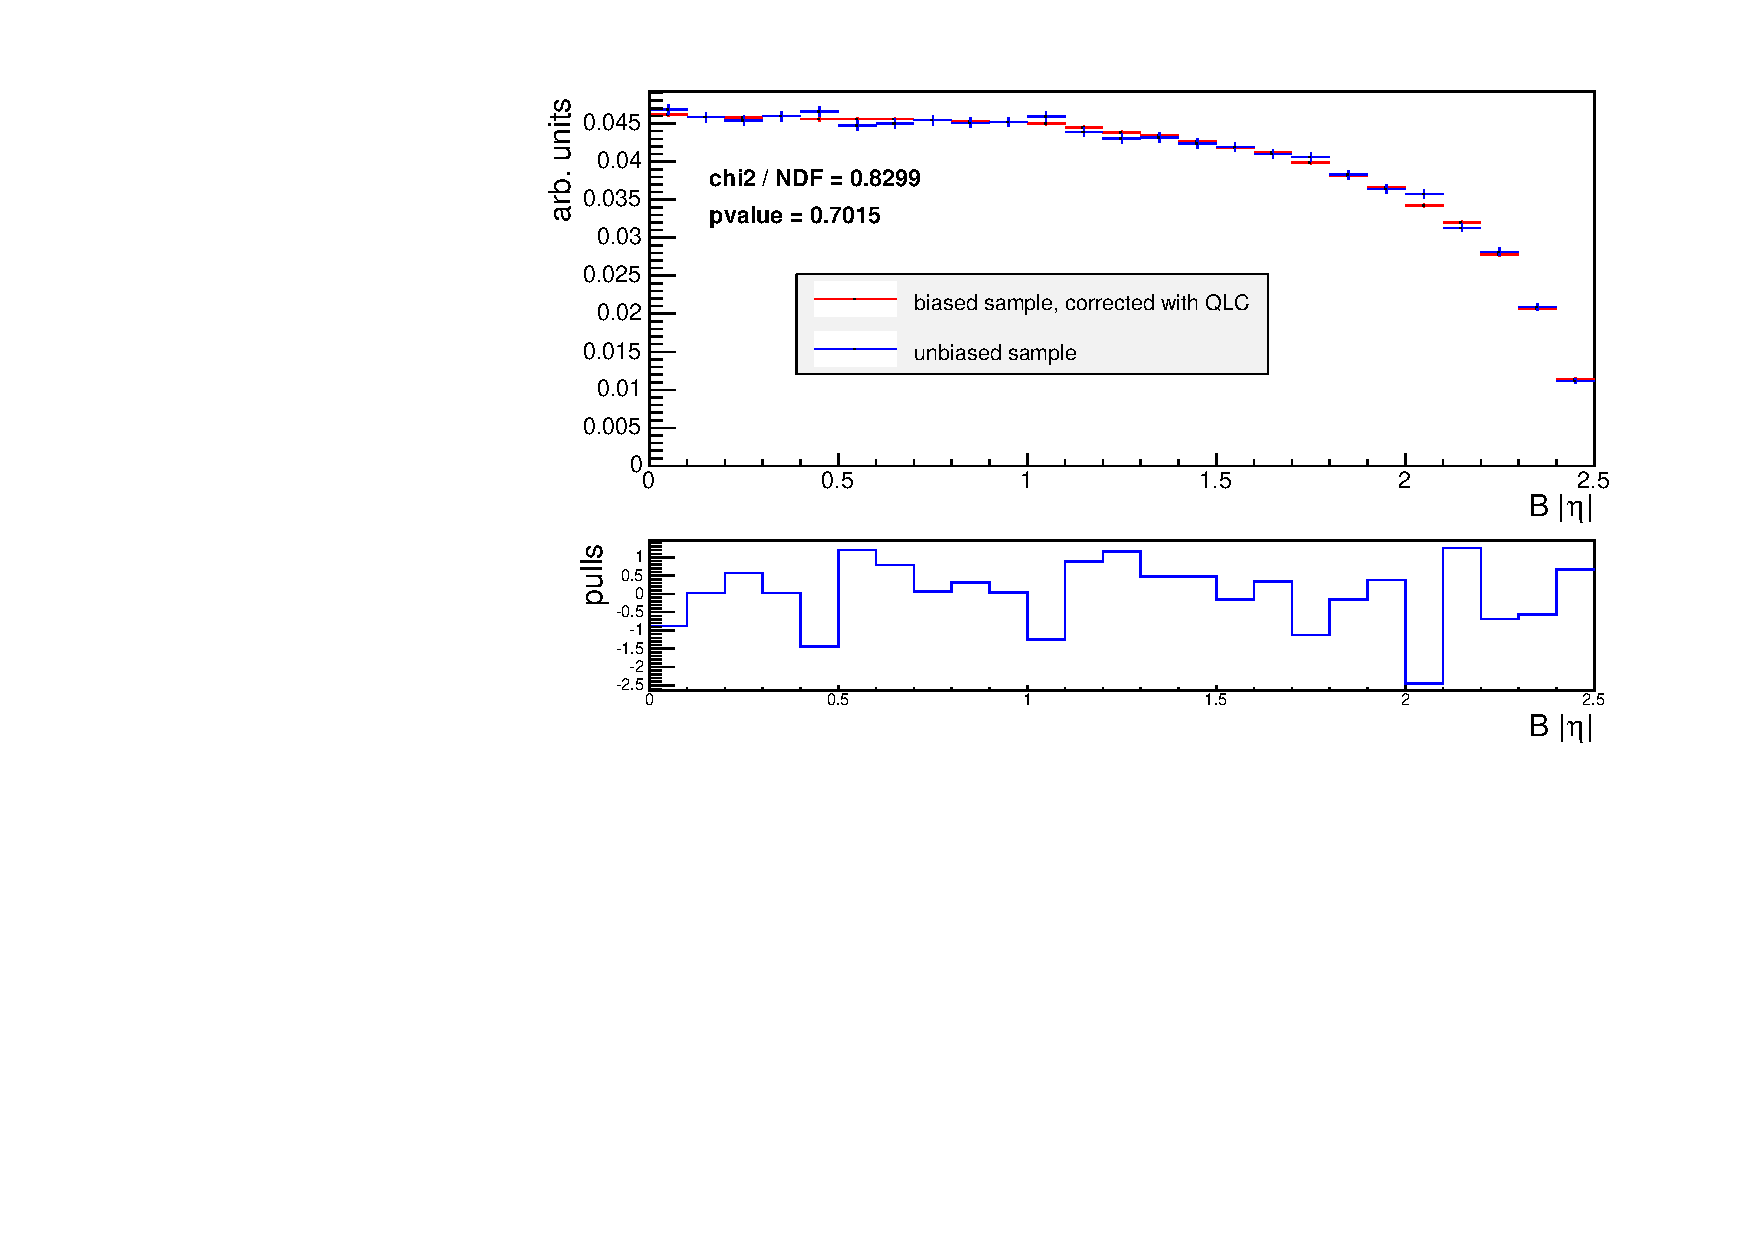
\includegraphics[width=15cm]{figures/InternalNote_MCTuning/oneSample_unbiasedVsQuarkBiasedComparison_eta.pdf}\\
%  \vspace{0.5cm}
%  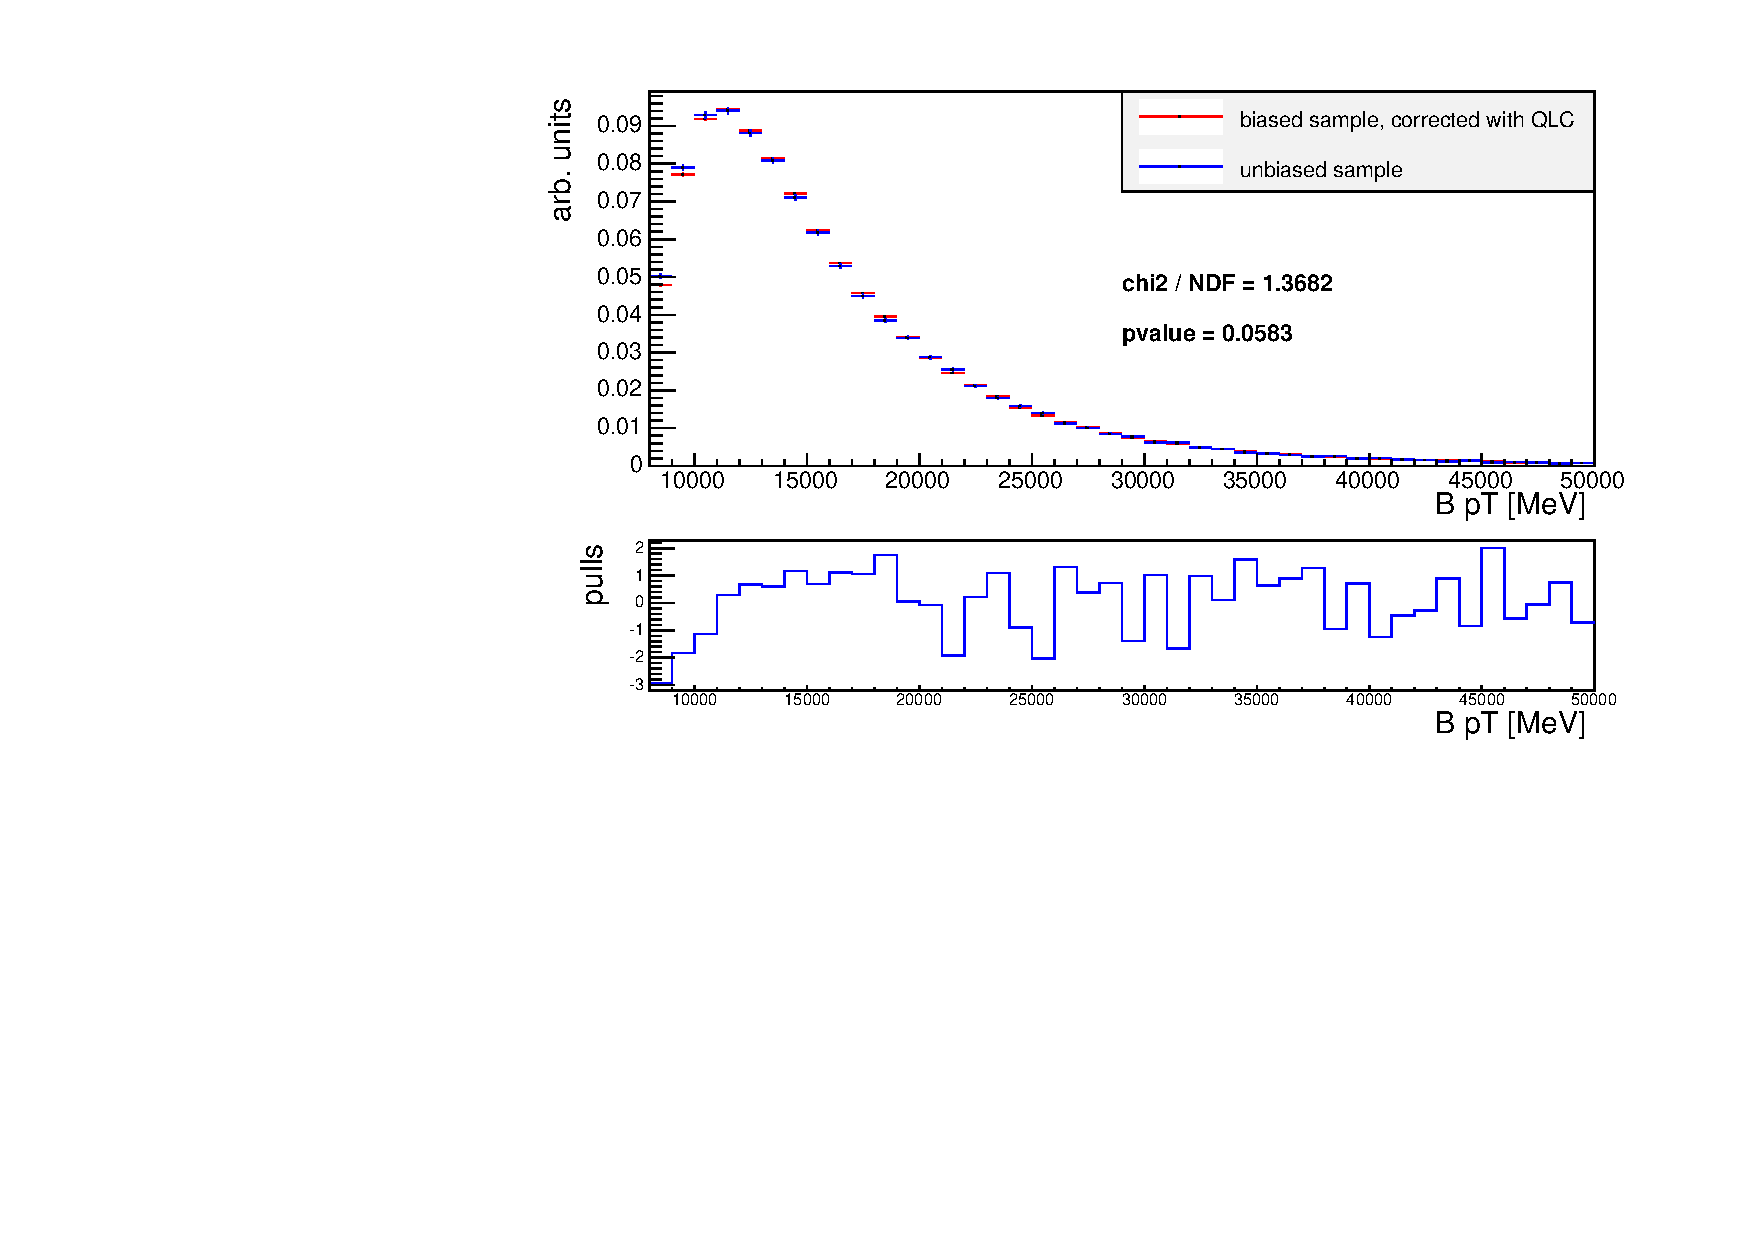
\includegraphics[width=15cm]{figures/InternalNote_MCTuning/oneSample_unbiasedVsQuarkBiasedComparison_pt.pdf}
%  \caption{Plots show the comparison of the $\eta_B$ (first plot) and $pT_B$ (second plot) QLC corrected quark biased distribution and the unbiased disttibution. In order to avoid correlations between the distributions, QLC have been calculated using odd numbered events from the unbiased sample and the QLC corrected quark biased distributions are compared with even numbered unbiased events.}
%  \label{fig:BpQLCapplied_oneSample}
%\end{figure}
%As a cross-check QLC calculated using odd events from the $B^+ \to J/\psi K^+$ unbiased MC have been applied to the quark biased sample and the result has been compared to the distribution of the even unbiased events \ref{fig:BpQLCapplied_oneSample}. The B meson $\eta$ distribution shows good agreement, while the pT distribution shows an inconsistency at low pT. The same effect is visible swapping odd and even unbiased events.\\
%The source of this discrepancy is due to the $\hat{pT}$ cut introduced at generator level, figure  \ref{fig:pTHatComparison_unbiasedVsSemiBiased} shows the $\hat{pT}$ distribution of the unbiased sample and the $\hat{pT}$ distribution from a new sample, semi biased, generated with the same cuts as the unbiased sample but with tigther $\hat{pT}$ (7. GeV instead of 5.), the distribution of the unbiased sample has been cut at 7 GeV in order to compare the two distributions, that are clearly not compatible.\\
%\begin{figure}[h]
%  \centering
%  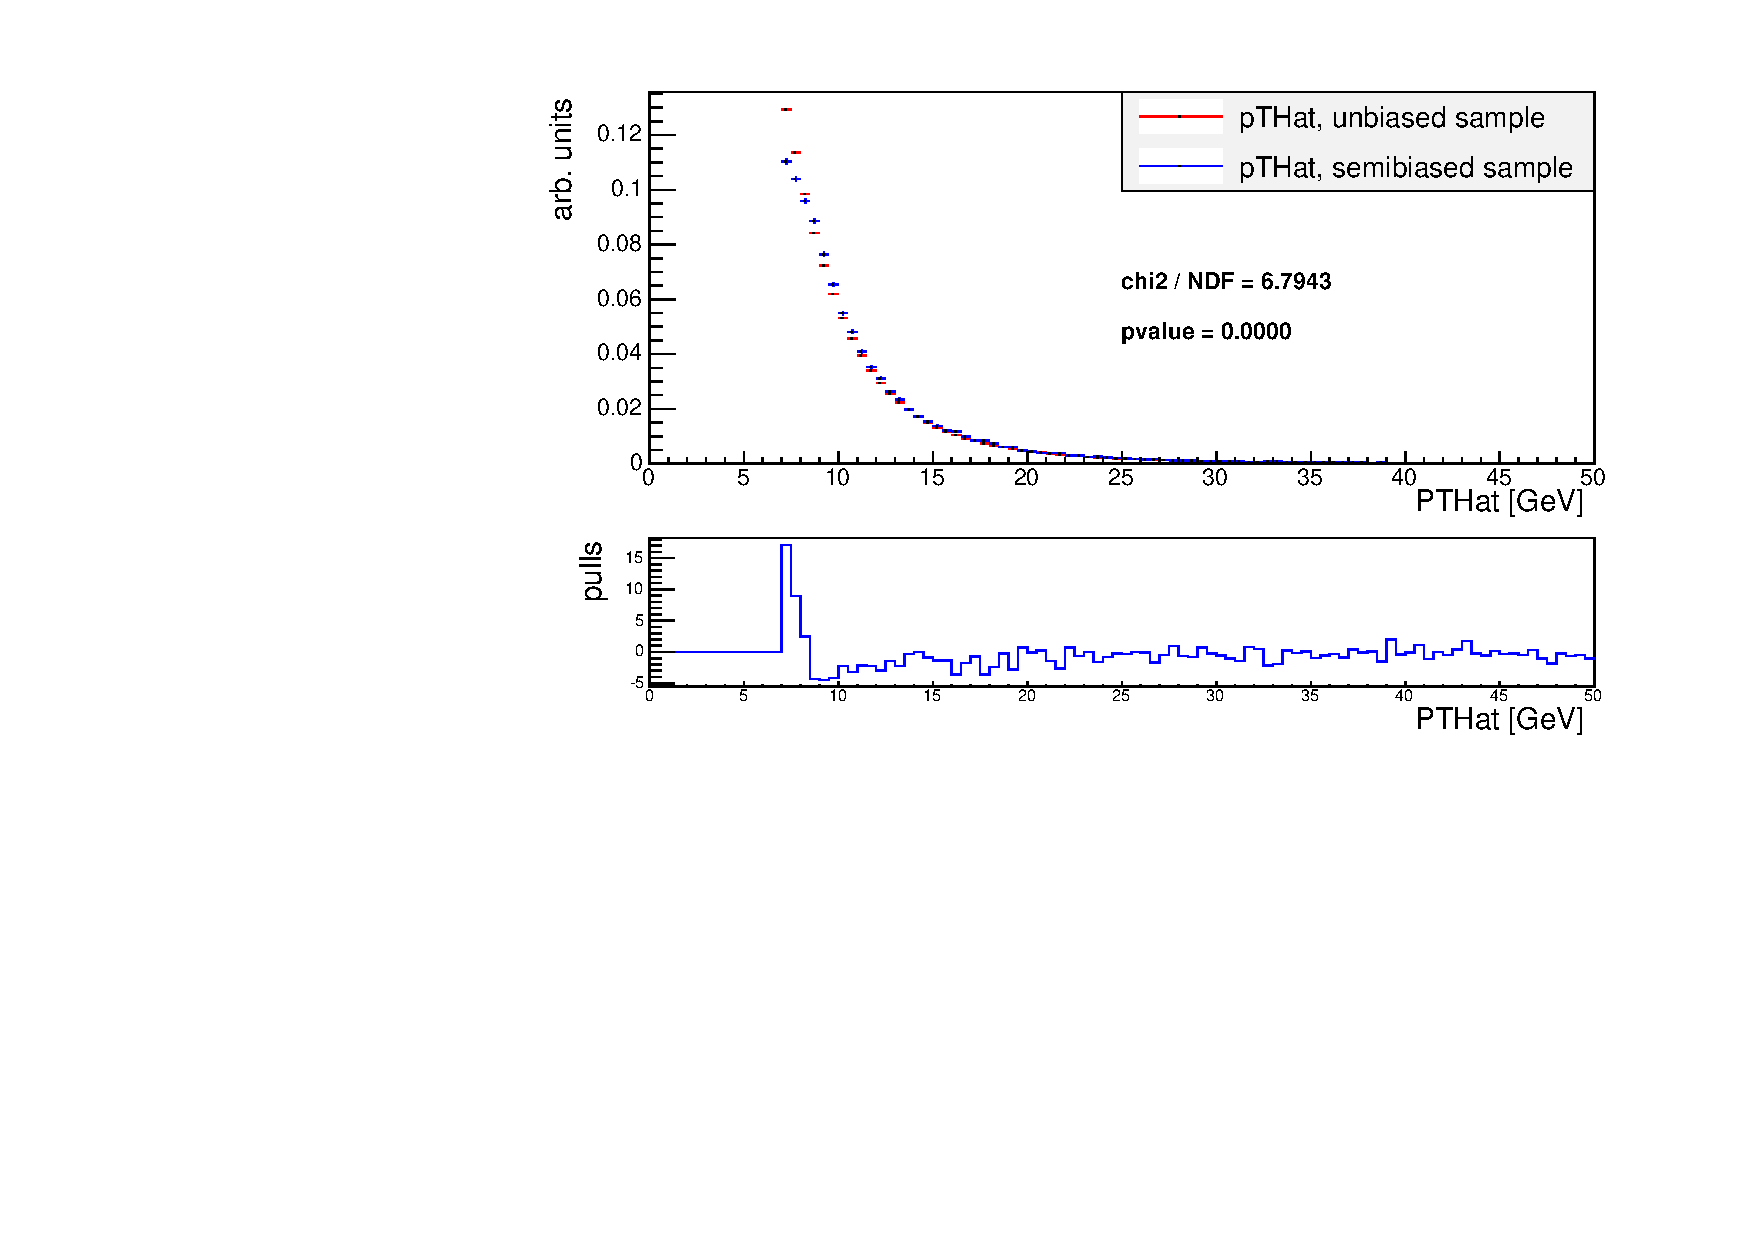
\includegraphics[width=15cm]{figures/InternalNote_MCTuning/PTHatComparison_UnbiasedVsSemiBiased.pdf}
%  \caption{Plot show the comparison of the $\hat{pT}$ distribution from the unbiased sample and the $\hat{pT}$ distribution from a new sample, semi biased, with the same quark-level cuts as the unbiased but with tighter $\hat{pT}$ (7 GeV insted of 5). The unbiased distribution has been cut at 7 GeV in order to compare the two distributions.}
%  \label{fig:pTHatComparison_unbiasedVsSemiBiased}
%\end{figure}
%This is due to a regularisation in the Pythia generation for low $\hat{pT}$ \yel[is the pythia manual in the bib files? not sure]{CITE PYTHIA MANUAL(page14)}; basically the parton-parton cross section becomes too high at low $\hat{pT}$, violating unitarity, this modification smoothly regulates the divergence. 
%QLC calculated using a single unbiased sample are therefore not usable, because they would introduce an additional bias due to this $\hat{pT}$ discrepancy.\\

The computation of the QLC is performed using the unbiased and 
the quark biased samples according to the following formula:
$$   W_{QL} = \nu^{FScuts}_{quarkBiased} \cdot \left(  \frac{\sigma^{Pythia}_{quarkBiased}}{N^{tot}_{quarkBiased}} \right) / \left[ \nu^{FScuts}_{unbiased} \cdot \left( \frac{\sigma^{Pythia}_{unbiased}}{N^{tot}_{unbiased}} \right) \right] $$  
Where $\nu$ is the number of entries in a ($pT_B$, $\eta_B$) from 
the unbiased or quark biased samples after applying the final state 
particle cuts. The term $ \frac{\sigma^{Pythia}}{N^{tot}}$ is used 
to normalise the two MCs to the same integrated 
luminosity: $\sigma^{Pythia}$ is the Pythia generation cross-section 
and $N^{tot}$ is the total number of generated events.\\
The inverse of these weights should be used to weight events 
individually, thus correcting with event-weights the QL cut biases.\\

%%%%%old considerations about the pTHat issue, might go into an appendix (as above)
%Before start calculating the QLC we have to make sure that the unbiased 
%sample we have is not affected by the $\hat{pT}$ bias. Figure 
%\ref{fig:pTHatComparison_unbiasedVsSuperUnbiased} shows the comparison 
%of the $\hat{pT}$ distribution from the unbiased sample and a new sample 
%with the same quark-level cuts as the unbiased but with looser 
%$\hat{pT}$ (3 GeV insted of 5), the distribution of the new sample has 
%been cut at 5 GeV in order to compare the two distributions. We are 
%interested in not having the bias in the parameter space used in the 
%analysis, therefore the quark-level cuts, final state cuts and B 
%fiducial volume cuts ($pT_B$ > 8 GeV and  $|\eta_B|$ < 2.5 ) are applied. 
%The two distributions look compatible, therefore we can use the unbiased sample for the QLC calculation.\\
%\begin{figure}[h]
%  \centering
%  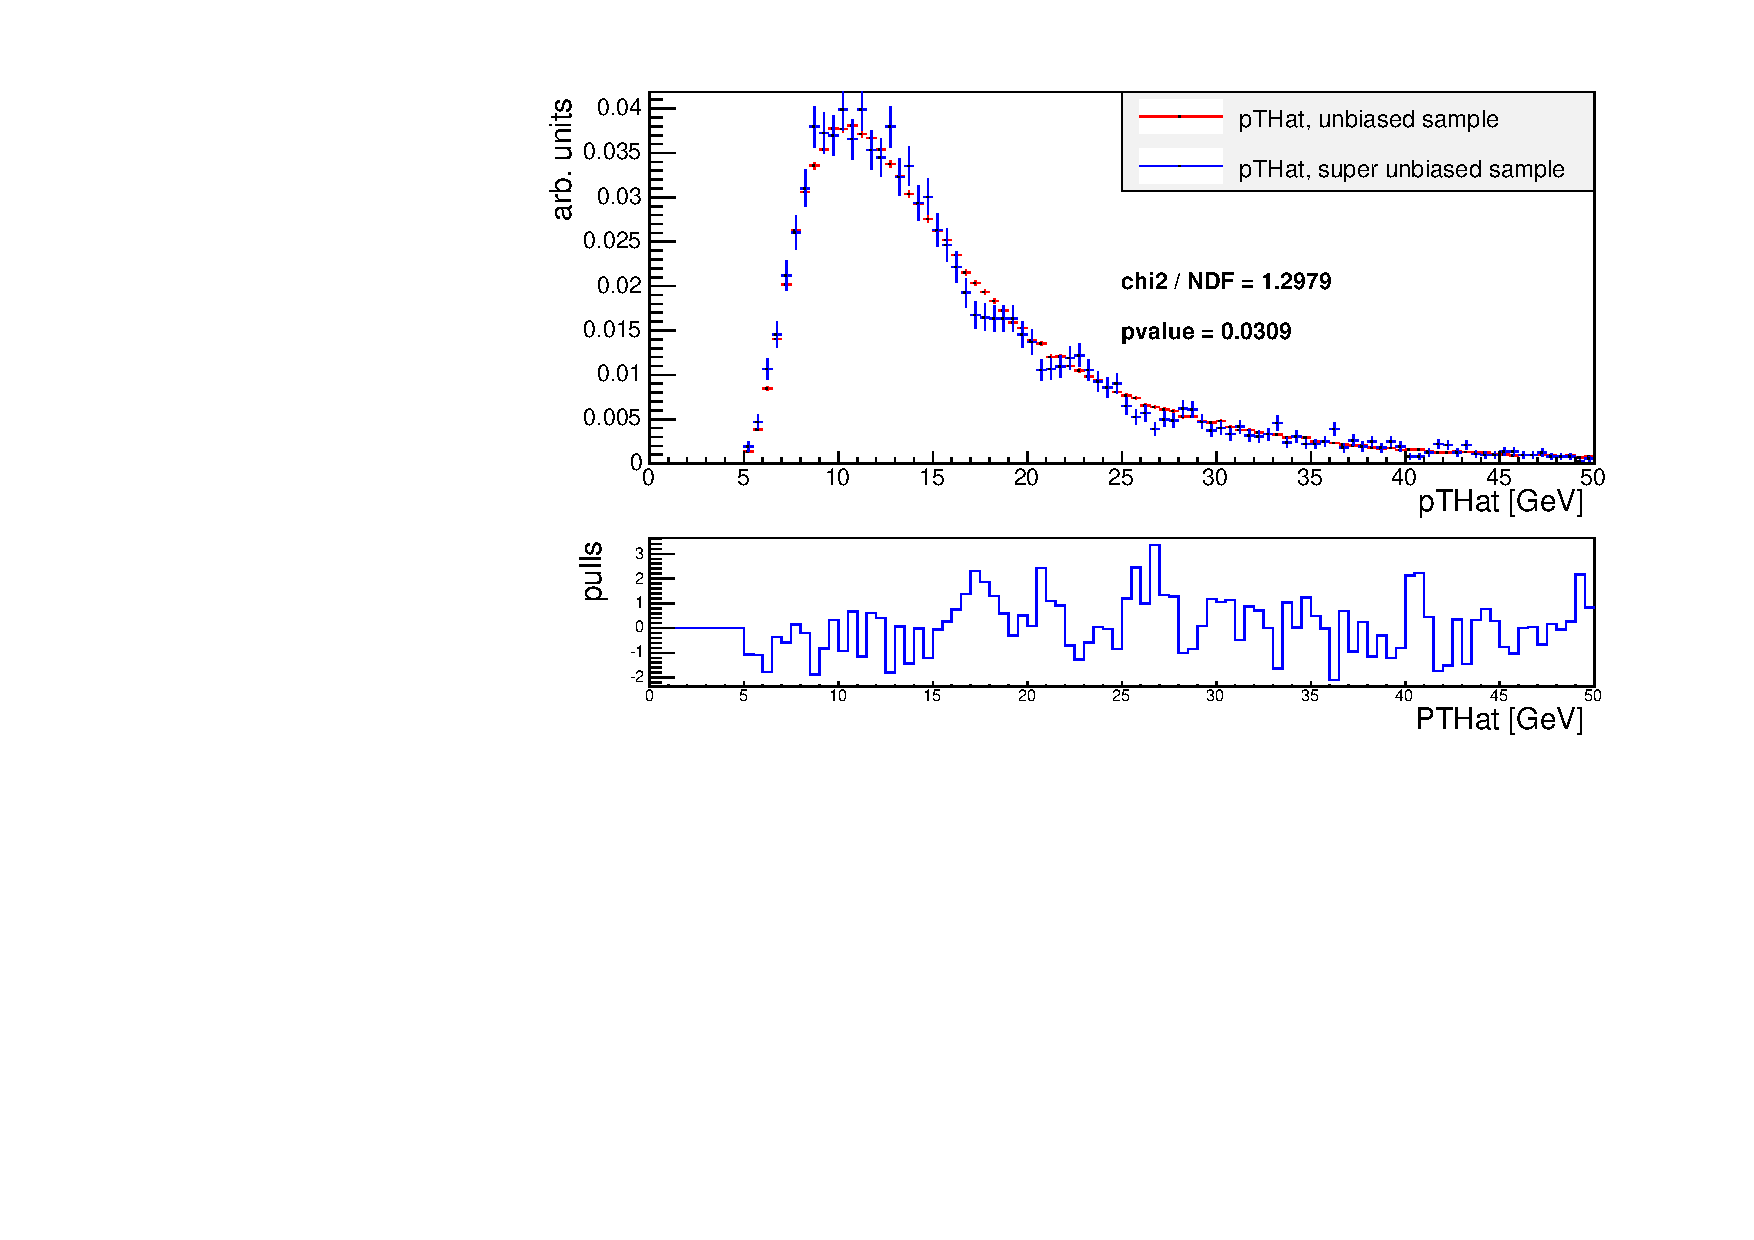
\includegraphics[width=15cm]{figures/InternalNote_MCTuning/pTHatComparison_unbiasedVsSUperUnbiased.pdf}
%  \caption{Plot show the comparison of the $\hat{pT}$ distribution from the unbiased sample and the $\hat{pT}$ distribution from a new sample, super unbiased, with the same quark-level cuts as the unbiased but with looser $\hat{pT}$ (3 GeV insted of 5). The super unbiased distribution has been cut at 5 GeV in order to compare the two distributions. Quark-level cuts, final state cuts and B fiducial volume cuts ($pT_B$ > 8 GeV and  $|\eta_B|$ < 2.5 ) are applied to both distributions.}
%  \label{fig:pTHatComparison_unbiasedVsSuperUnbiased}
%\end{figure}

Figure~\ref{fig:allQLC}  \yel[B+ QLC ready, BsMuMu and BsJpsiPhi QLC still work in progress]{show the QLC calculated for $B^+$, $B_s \rightarrow \mu \mu$, and $B_s J/\psi \phi$  and their uncertainty}.
This computation of the QLC has been cross-check applying 
QLC calculated using odd events, from both the quark biased and 
unbiased samples, to the even events of the quark biased sample. 
The resulting distributions have been compared to unbiased 
distributions obtained using only even events. 
%The inconsistency at low pT has now disappeared, 
Figure \ref{fig:BpQLCapplied_twoSample} 
shows the checks performed on the $B^+$ sample.
\begin{figure}[h]
  \centering
  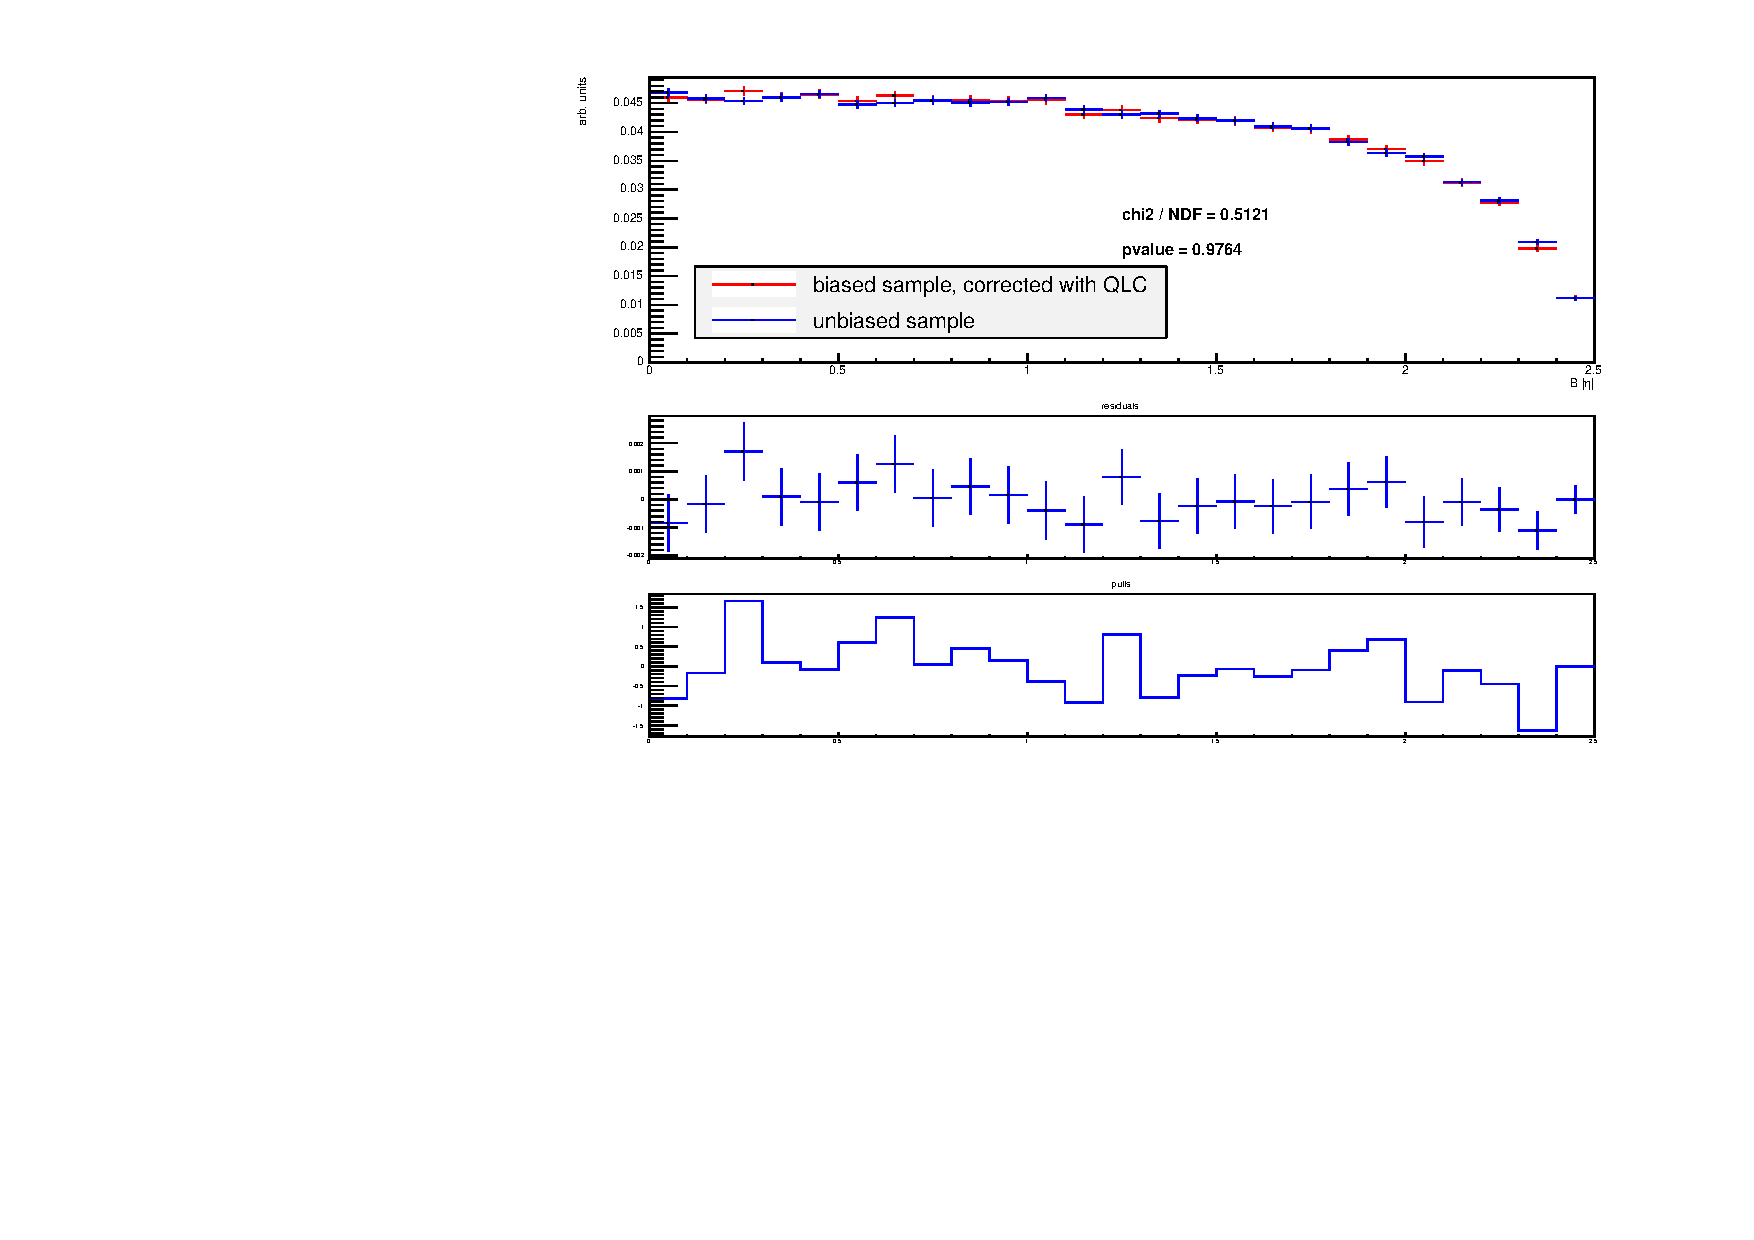
\includegraphics[width=15cm]{figures/InternalNote_MCTuning/twoSampleApproachApplication_etacomparison.pdf}\\
  \vspace{0.5cm}
  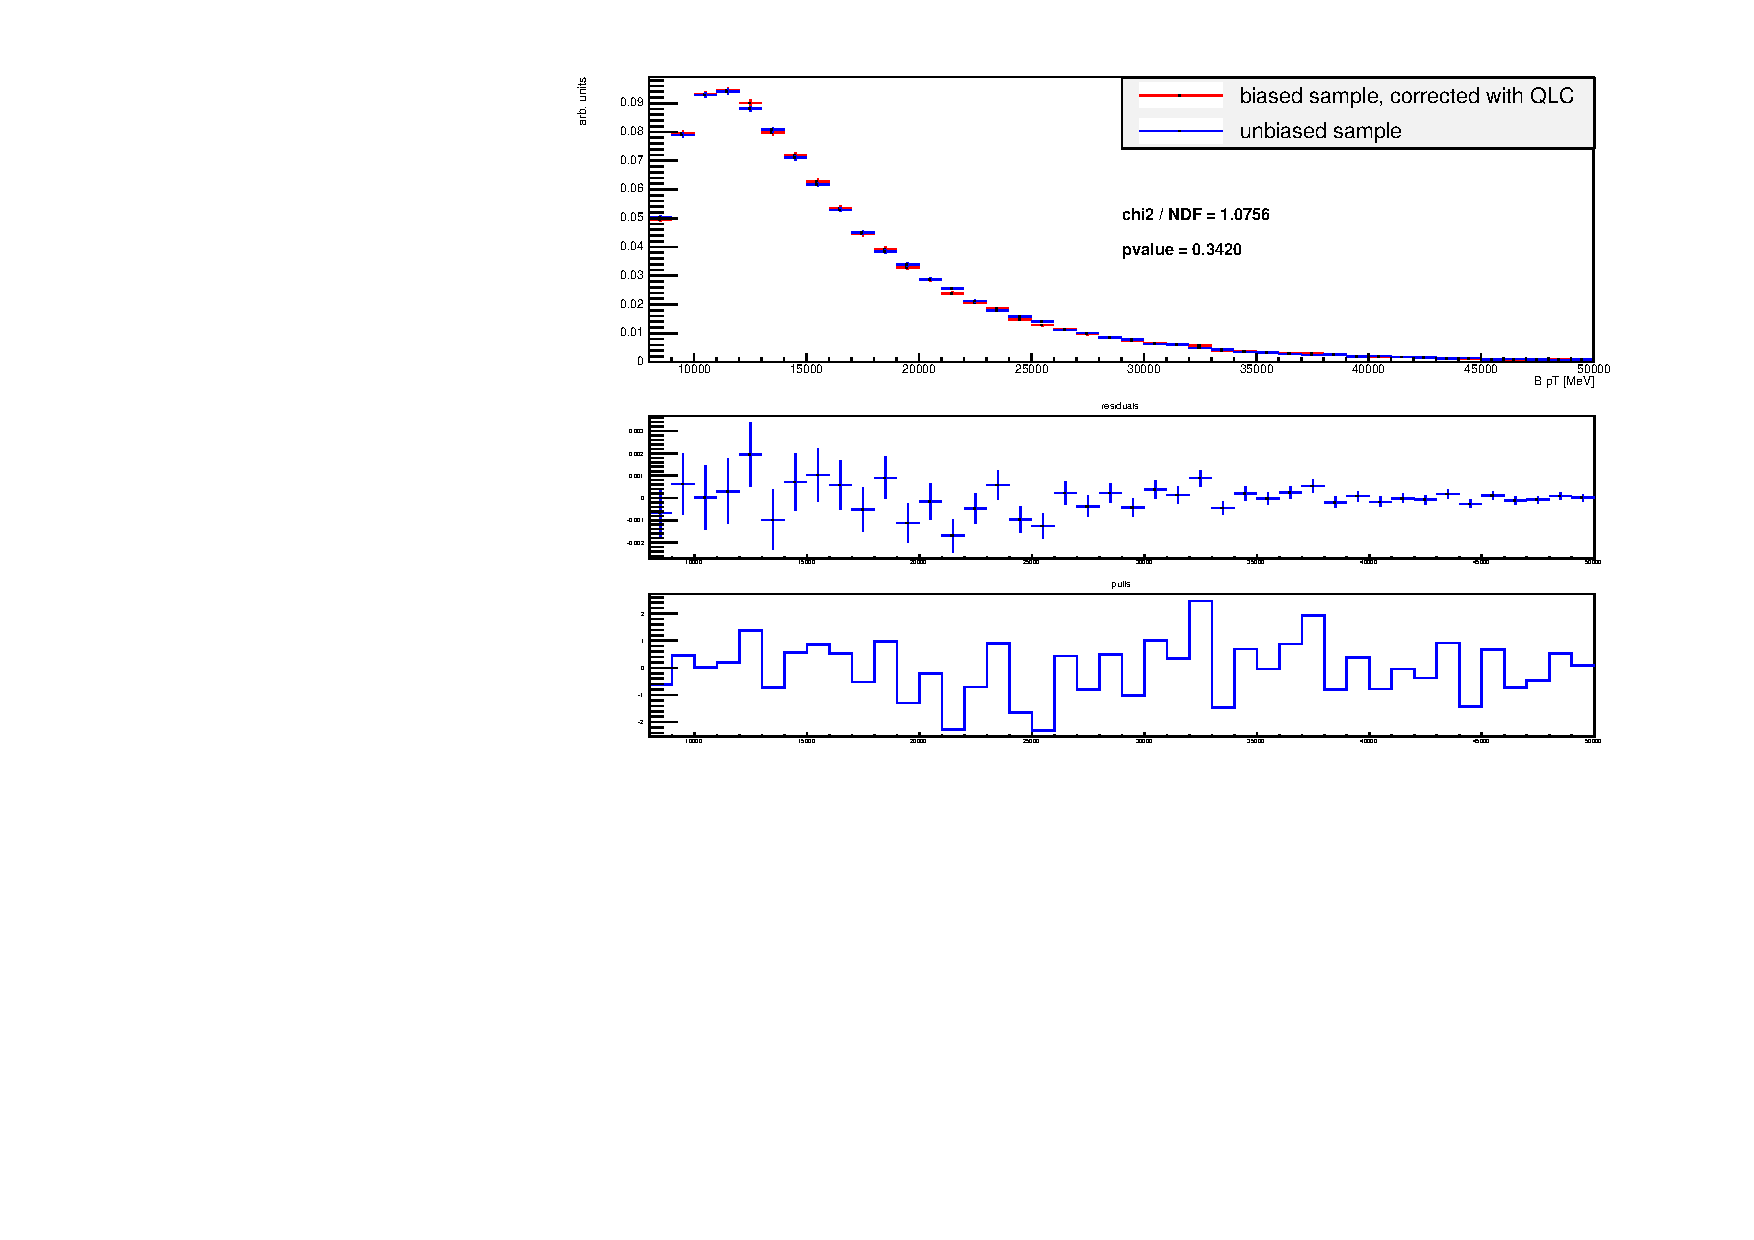
\includegraphics[width=15cm]{figures/InternalNote_MCTuning/twoSampleApproachApplication_pTcomparison.pdf}
  \caption{Plots show the comparison of the $\eta_B$ (first plot) and $pT_B$ (second plot) QLC corrected quark biased distribution using the two samples approach QLC and the unbiased distribution. In order to avoid correlations between the distributions, QLC have been calculated using odd numbered events from the unbiased and quarkBiased samples, and the remaining events in the two samples have been weighted and used for the comparison.}
  \label{fig:BpQLCapplied_twoSample}
\end{figure}











\subsection{Data Driven Weights}
\label{sec:ddw}

The Data Driven Weights (DDW) have been evaluated in a similar way as it 
has been done in~\cite{bsmumuv2} and ~\cite{Alpigiani:1756291}.\footnote
{Due to the limited statistics of the $B^+$ data sample, 
the DDW corrections are not computed in a two-dimensional
grid of the variables $p_T$ and $|y|$, but are extracted with the one-dimensional times %$\times$
one-dimensional procedure described in the text. 
This approach was already used in the analyses~\cite{bsmumuv2} based on 
the 4.7~fb$^{-1}$ sample of data collected in 2011 and~\cite{Alpigiani:1756291} based on the
full Run1 sample.
The validity of the approach is tested by the stability of the recursive procedure,
and fundamentally it works because the production cross-section depends strongly
on $p_T$, but much less on $|y|$, with small correlation
between the two variables. The systematic deviation in the computation of the
average acceptance times %$\times$ 
efficiency due to the method chosen for this analysis
rather than a true two-dimensional computation of the DDW has been estimated
to be at the level of \yel[still work in progress]{.......}
}

The DDW for the MC signal samples are determined with an iterative method,
by comparing sideband-subtracted $B^\pm\to J/\psi K^\pm$ odd-numbered
events with MC events, after the latter are corrected with the $W_\mathrm {QLC}$ weights.\footnote
%
%
{The extraction followed similar lines used in \cite{bsmumuv2} and ~\cite{Alpigiani:1756291}.  
The \Bp yeld was extracted in \pt intervals and alternatively, in $|\eta|$ intervals.
The event selection followed the same line discussed in the following sections of this note, with the addition of 
an additional cut $L_{xy}>0.3$~mm on the transverse separation between primary and secondary vertex, and
without applying the multivariate selection against combinatorial background. The signal is described with
two Gaussians with equal mean; the continuum background is described by an exponential; 
the background due to partially reconstructed decays ($B$ to $J/\psi\, X$, with m($J/\psi \, h^+<5.200$~GeV)  
is described with an error function.
All shape and amplitude parameters are extracted form the fit, and the uncertainty in the signal yield is dominated 
statistical errors. }

We derive two sets of weights, in $\pt$ and $|\eta|$ of the $B$ meson,
determined by the ratio of the normalised $\pt$ and $|\eta|$ spectra
in data and MC.
The final weights that are going to be used are therefore
\begin{equation}
W_\mathrm {DD}\left(\pt,|\eta|\right)=w\left(\pt\right)\cdot w\left(\eta\right)\label{for:ddw}
\end{equation}
where $w={\nu^{data}}/({\nu^{MC}}\times W_\mathrm {QLC})$ and $\nu$ is the normalised
number of entries in either the data or MC histograms for $\pt$ or $\eta$.
\yel[calculaton of DDW underway]{These weights are then used as per-event weights on the MC events, and the
procedure is iterated until these weights stabilise. The stability of the
weights can be seen from the convergence of the second iteration
and it is shown in Figure .....}


%\begin{figure} [!htp]
%  \begin{center}
%  \includegraphics[width=0.88\textwidth ]{eps/glc/ddwCombo_2012_MC2Weighted_withQLC.eps}
%  \caption{
%  {\it Top\/} :DDW extracted for $B^\pm \to J/\psi K^\pm$ as function of $\pt$ ({\it left}) and $\eta$ ({\it right}) of the $B$ meson. 
%    {\it Bottom\/}: the same as above showing the separately the result of the first iteration (blue points) 
%    and the small additional correction (red points) from the second iteration.
%    }
%  \label{fig:ddwBplus}
%  \end{center}
%\end{figure}




%Events from \Bs \ decays into $J/\psi\, \phi \to \mu^+\mu^-\K^+\K^-$ can be studied
%and compared to \Bp \ decays to $J/\psi \,K^+$.  In particular, DDW can be extracted in the
%$J/\psi\, \phi $ channel and compared the standard ones from  $J/\psi K^+$.
%This is shown in Figure~\ref{fig:ddwJPsiPhi}.\footnote
%{Here the data points for \Bp \ were obtained without reweighting the MC sample
%according to the pre-L2StarB and L2StarB trigger configuration and without applying data-driven
%corrections to the trigger efficiency, causing a minor
%difference from the plot in Figure~\ref{fig:ddwBplus}. The treatment was consistent
%between the two channels, and the comparison is not significantly affected.}
%The two sets of weights agrees well within the the statistical error, confirming
%that the relative yield of \Bs \ and \Bp does not to depend significantly on \pt \
%and \eta ~\cite{Aaij:2013qqa, lhcbfsfu14}, and providing a consistency check on our
%procedures. Furthermore, the comparison supports the assumption of using DDW derived
%from \Bp \ also  for the \Bs \ channel. 
%\begin{figure} [!htp]
%  \begin{center}
%  \includegraphics[width=0.65\textwidth ]{eps/glc/compare_JpsiPhi_JpsiKplus_MC1Weighted.eps}
%  \caption{
%  Comparison of DDW for $\Bp \to J/\psi K^+$ (blue points) and $\Bs \to J/\psi \phi$ (red points).}  
%  \label{fig:ddwJPsiPhi}
%  \end{center}
%\end{figure}


\clearpage

%% preselection
\section{Candidate Preselection}
\label{sec:Preselection}

\subsection{Candidate building and preselection on derivation level}
\label{ssec:CandidateBuildingByDerivation}

For the Run~2 \Bmumu\ analysis the \Bds\ and \Jpsi\ candidates are build
simultaneously by the derivation format \texttt{BPHY8} (for data and continuum
background) in the three relevant decay modes:
\begin{itemize}
\item \Bmumu\ signal channel\\
  A \Bds candidate is build from two oppositely-charged muons.  
  Before vertexing the muon momenta are corrected by the 
  \texttt{MuonCalibrationAndSmearingTool} as
  recommended by the muon combined performance group, applying the 
  appropriate configurations\footnote{
    %% w.w., 2018-04-13:
    %% Please note that these are already the updated settings for
    %% the upcoming re-processing of all our DAODs.
    For data15: 
    \texttt{McstYear = ``Data15''}, 
    \texttt{McstRelease = ``Recs2017\_08\_02''},
    \texttt{McstStatComb = False},
    \texttt{McstSagittaCorr = True},
    \texttt{McstSagittaRelease = ``sagittaBiasDataAll\_25\_07\_17''},
    \texttt{McstDoSagittaMCDistortion = False};\newline
    for data16:
    \texttt{McstYear = ``Data16''}, 
    \texttt{McstRelease = ``Recs2017\_08\_02''},
    \texttt{McstStatComb = False},
    \texttt{McstSagittaCorr = True},
    \texttt{McstSagittaRelease = ``sagittaBiasDataAll\_25\_07\_17''},
    \texttt{McstDoSagittaMCDistortion = False};\newline
    for MC the data16 settings are applied.
  }
  for data15 and data16.
  Using the \texttt{JpsiFinder} tool, the \Bds\ candidates are 
  constructed by a fit of the two muon's inner detector tracks to a
  common vertex requiring $\chi^2_{\Bds}/NDF < 15$ and $3500~\mathrm{MeV} 
  < m_{\Bds} < 7000~\mathrm{MeV}$.  In addition, the so called
  muon-based mass $m^{\mathrm{MUCALC}}_{\Bds}$ and the corresponding 
  uncertainty are calculated as the invariant
  mass from the four-momentum sum using the combined muon
  information of the two muons comprising the candidate.  The
  PDG-mass for muons is applied in this calculation.
  On data, the candidates two mass values are 
  \yel[The footnote text already explains the new blinding method
  with the encrypted mass values.]{blinded}\footnote{
    The mass values are encrypted using a simple RSA algorithm with 
    asymmetric keys, multiplied by $-1$, so that they 
    appear on the negative side of the mass spectrum, 
    and stored in the same float variable.
  }
  if both, $m_{\Bds}$ and $m^{\mathrm{MUCALC}}_{\Bds}$ fall into the blinded
  region around the nominal $\Bs$, i.e. into the interval from
  5166~MeV to 5526~MeV.
\item \BpmKpmJpsi\ reference channel with \JpsiMuMu\\
  First \Jpsi\ candidates are reconstructed using the
  \texttt{JpsiFinder} similarily as for the \Bmumu\ signal channel
  with an adjusted mass range of
  $2000~\mathrm{MeV} < m_{\Jpsi} < 7000~\mathrm{MeV}$.
  Then the \texttt{JpsiPlus1TrackFinder} tool is used to combine the \Jpsi\ 
  candidates with an additional track\footnote{
    We apply the BLS group's standard inner detector track preselection
    for vertexing as defined in \texttt{configureVertexing.py}, among
    them 
    \texttt{pTMin = 400.0}~MeV,
    and the minimal track hit requirements
    \texttt{nHitBLayer = 0}, 
    \texttt{nHitPix = 1},
    \texttt{nHitBLayerPlusPix = 1},
    \texttt{nHitSct = 2},
    \texttt{nHitSi = 3},
    \texttt{NHitTrt = 0} 
    as well as
    \texttt{TrtMaxEtaAcceptance = 1.9}.
  }
  which is required to have  
  $\pt^{Jpsi} > 1$~GeV and $|\eta < 2.5|$.  A mass constraint of the \Jpsi\
  candidate's mass to the \Jpsi\ PDG mass is applied. 
  The \Bpm\ candidates are 
  accepted if $\pt^{\Bpm} > 1$~GeV, $\chi^2_{\Bpm}/NDF < 15$ and
  $3500~\mathrm{MeV} < m_{\Bpm} < 7000~\mathrm{MeV}$.
  Again, muon-based mass values $m^{MUCALC}_{\Bpm}$ and corresponding 
  uncertainties are calculated
  from the four-momenta of the two muons and the additional kaon
  track, assuming PDG values for the masses of the muons and the kaon
  as appropriate.  No mass-value blinding is applied to the reference
  channel candidates.
\item \BsJpsiPhi\ control channel with \JpsiMuMu\\
  To reconstruct \BsJpsiPhi\ candidates, the \Jpsi\ candidates
  reconstructed as described for the  \BpmKpmJpsi\ channel above are
  combined with two oppositely-charged inner detector tracks
  fulfilling the same requirements as the kaon track in the
  \BpmKpmJpsi\ reconstruction by the \texttt{JpsiPlus2TracksFinder}
  tool. Again, a mass constraint of the \Jpsi\ candidate's mass to the
  \Jpsi\ PDG mass is applied.
  Muon-based mass values $m^{MUCALC}_{\Bs}$ and corresponding 
  uncertainties are calculated
  from the four-momenta of the two muons and the two additional kaon
  tracks, assuming PDG values for the masses of the muons and the kaons
  as appropriate.  No mass-value blinding is applied to the control
  channel candidates.
\end{itemize}

For MC signal channels only the relevant decay modes are run.  For
the \Bhh\ MC the requirement that the inner detector tracks must be
identified as muons is dropped. Instead two oppositely-charged tracks
with $\pt > 3.5$~GeV and $|\eta| < 2.5$ are required.
For the \BpPipJpsi\ Monte Carlo sample, two instances of the
\BpmKpmJpsi\ mode are run in parallel.  The first one is assuming the
PDG pion mass for the additional track, while the second one assumes
the (wrongly-assigned) PDG kaon mass.  The second version is needed as
-- due to the lack of pion-kaon separation in ATLAS -- 
our \BpmKpmJpsi\ reference sample on data will contain a contribution
of \BpPipJpsi\ events located to the right of the \Bpm\ peak 
due to the wrongly-assigned mass values for the pion track.

At derivation level each $B$ and $\Jpsi$ candidate is decorated with
the additional information about e.g. the separation w.r.t. the associated 
primary vertex (see Section~\ref{subsec:PVdetermination}), 
the isolation of the candidate and others:
\begin{itemize}
\item Isolation of the decay candidate $I_{0.7}$ and 
  number of tracks around the candidate $N^{trks}_{0.7}$\\
  Both variables are defined in Table~\ref{tab:15vars}.  Only 
  tracks of the CP-type ``loose'' being part of the primary vertex 
  associated to the secondary vertex and tracks not associated to any
  primary vertex are taken into acount.  The tracks which are not part
  of the secondary vertex candidate are required to
  have $\pt > 0.5$~GeV and to stem 
  from within a cone of $\Delta R < 0.7$ around the $B$ candidates
  momentum vector.  The tracks considered also need to be close enough
  to the primary vertex, i.e. $\log\chi^2_{DCA} < 5$ where
  \[ 
  \log\chi^2_{DCA} = \log\left(\left(\frac{d_0}{\sigma_{d_0}}\right)^2 
    + \left(\frac{z_0}{\sigma_{z_0}}\right)^2\right)
  \]
  with the transverse and longtidinal impact parameters $d_0$ and 
  $z_0$ respectively.
  $N^{trks}_{0.7}$ records the number of non-decay-candidate tracks
  within the cone.
\item Isolation of the muons $I_{0.7}^{\mu_i}$ and
  number of tracks around the muons $N_{0.7, \mu_i}^{trks}$\\
  Similar to the isolation variables for the decay candidate,
  $I_{0.7}^{\mu_i}$ are calculated as the isolation values for 
  the two muons within a cone of $\Delta R<0.7$ around each muon's
  momentum vector w.r.t. inner detector tracks.  The number of 
  tracks within the cone is recorded by $N_{0.7, \mu_i}^{trks}$.
\item Closest track to the vertex candidate and number of close
  tracks $N^{close}_{trks}$\\
  Link to the track closest to the decay vertex candidates from 
  the set of tracks fulfilling the same requirements as for the
  determination of the isolation variable except for the 
  missing cone size requirement and an adjusted  
  $\log\chi^2_{DCA} < 7$ cut.
  In addition the number of all qualifying closest track candidates
  with $\log\chi^2_{DCA,SV} < 1$ is recorded as  $N_{0.7,
    \mu_i}^{trks}$ where $\log\chi^2_{DCA,SV}$ is calculated w.r.t.
  the secondary vertex' position.
\item \texttt{minLogChi2ToAnyPV}\\
  The minimum distance in $\chi^2$ of the candidate to any primary
  vertex, using the refitted primary vertices associated to 
  reconstructed secondary vertices where existing.
\item Transverse, longitudinal and 3-dimensional impact parameters 
  w.r.t. the associated primary vertex and corresponding uncertainties
\item Transverse decay distance $L_{xy}$ w.r.t. the associated primary
  vertex and its uncertainty\\
  See Table~\ref{tab:15vars} for the definition of $L_{xy}$.
\item Proper decay time $\tau$ and its uncertainty
\end{itemize}

Only events with at least one decay candidate in one of the three
decay modes are stored in the derivation output (DAOD) file.  In order to
save disk space on the computing grid, from the
primary vertex collection only primary vertices associated to decay
vertices by the primary vertex assocation method (see
Section~\ref{subsec:PVdteermination} are saved. 
The muon collection and track collections are thinned to only contain
muons or tracks which are either part of a reconstructed decay vertex,
part of an associated primary vertex or identified as a track closest
to a decay vertex.
 

%-------------------------------------------------------------------------------

\subsection{Primary vertex determination}
\label{subsec:PVdetermination}
In full Run1 analysis a new approach to determine the primary vertex (PV) associated to the B candidate was developed, in order to exploit it also in Run2 its performance has to be tested again.
The Run1 approach performance has been compared to other three possible methods, in order to check for possible improvements. The 4 approaches considered are:
\begin{itemize}
\item PV\_MAX\_SUM\_PT2: predefined in ATLAS, considers the sum of the squared transverse momentum of the tracks associated to each PV, the chosen PV is the one with the highest sum;
\item PV\_MIN\_A0: a backward extrapolation of the B momentum from the decay vertex is considered, the PV is chosen as the one with the shortest 3D distance from the point of closest approach (POCA) of the B extrapolation to each of the reconstructed PVs;
\item PV\_MIN\_Z0: similar to PV\_MIN\_A0, but uses the distance along z from the POCA of the B extrapolation to each of the reconstructed PVs;
\item PV\_MIN\_Z0\_BA: approach developed for full Run1 analysis, the associated PV is chosen as the one with the shortest separation, along z, from the POCA of the B extrapolation to the beam line.
\end{itemize}
The performances of the four PV association procedure have been tested on signal MC sample.\\
A first comparison was performed using only the information regarding the coordinates of the selected PVs and the position of the truth PV.\\
Figures \ref{fig:PVSVass_xydist} and  \ref{fig:PVSVass_zdist} show respectively the distance on the xy plane and along the z direction between the selected PV and the truth PV for the four approaches.
PV\_MAX\_SUM\_PT2 shows clearly large distributions, which tells that the selected PV is often the wrong one. The other three approaches show almost identical narrow distributions.\\
In order to have a quantitative estimation of the performance of the approaches, for each PV reconstructed in the events, a $\chi^2$ is computed to estimate the compatibility with the MC truth. The PV with the lowest $\chi^2$ in each event is found to correspond to the PV correctly associated to the B candidate and is considered “truth-matched”. Figure \ref{fig:Chi2DistAndMatched} shows the distribution of the $\chi^2$ of all the PVs (blue points) and the distribution of the $\chi^2$ of the “truth-matched” PVs.
Figure \ref{fig:selectedChi2AndMatched} shows the distribution of the chosen PVs using the 4 approaches (green distributions) superimposed to the truth-matched distribution (red). While the distribution of chosen PVs for PV\_MAX\_SUM\_PT2 shows two clear peaks, that can be identified as correct associations (left peak) and wrong associations (right peak), the other three distributions show one peak that follows the behaviour of the “truth-matched” vertices.
Table \ref{table:PVpurity} shows the purity for each approach, defined as the ratio between the number of correct associations and the total number of candidates.
\begin{table}[h]
  \begin{center} 
    \begin{tabular}{| c | c |}
      \hline
      approach & purity  \\ \hline
      PV\_MAX\_SUM\_PT2	 & $0.451	\pm 0.0053$  \\ \hline
      PV\_MIN\_A0	 & $0.9938	\pm 	0.0008$  \\ \hline
      PV\_MIN\_Z0	 & $0.9937	\pm 	0.0008 $ \\ \hline
      PV\_MIN\_Z0\_BA	& $0.9931		\pm 0.0009 $ \\ 
      \hline
    \end{tabular}
    \caption{purity of the four considered approaches to perform PV-SV association}
    \label{table:PVpurity}  
  \end{center}
\end{table}
As expected, purity for PV\_MAX\_SUM\_PT2 is low, while for the other approaches the purities are compatible within the error.
Due to the increasing pile-up environment in Run2, we checked the stability of the four approaches as a function of the number of reconstructed primary vertices in each event (which is a good proxy for the pile-up).
Figure \ref{fig:purityFuncNPV} shows the result of this study. PV\_MAX\_SUM\_PT2 shows a remarkable dependence on the number of PVs, while the other approaches are stable.
Given the lack of significant improvements with the new approaches and aiming for minimal changes on the analysis approach, we decide to stick to the same algorithm used in the last round of the analysis (PV\_MIN\_Z0\_BA).

\begin{figure}[h]
  \centering
  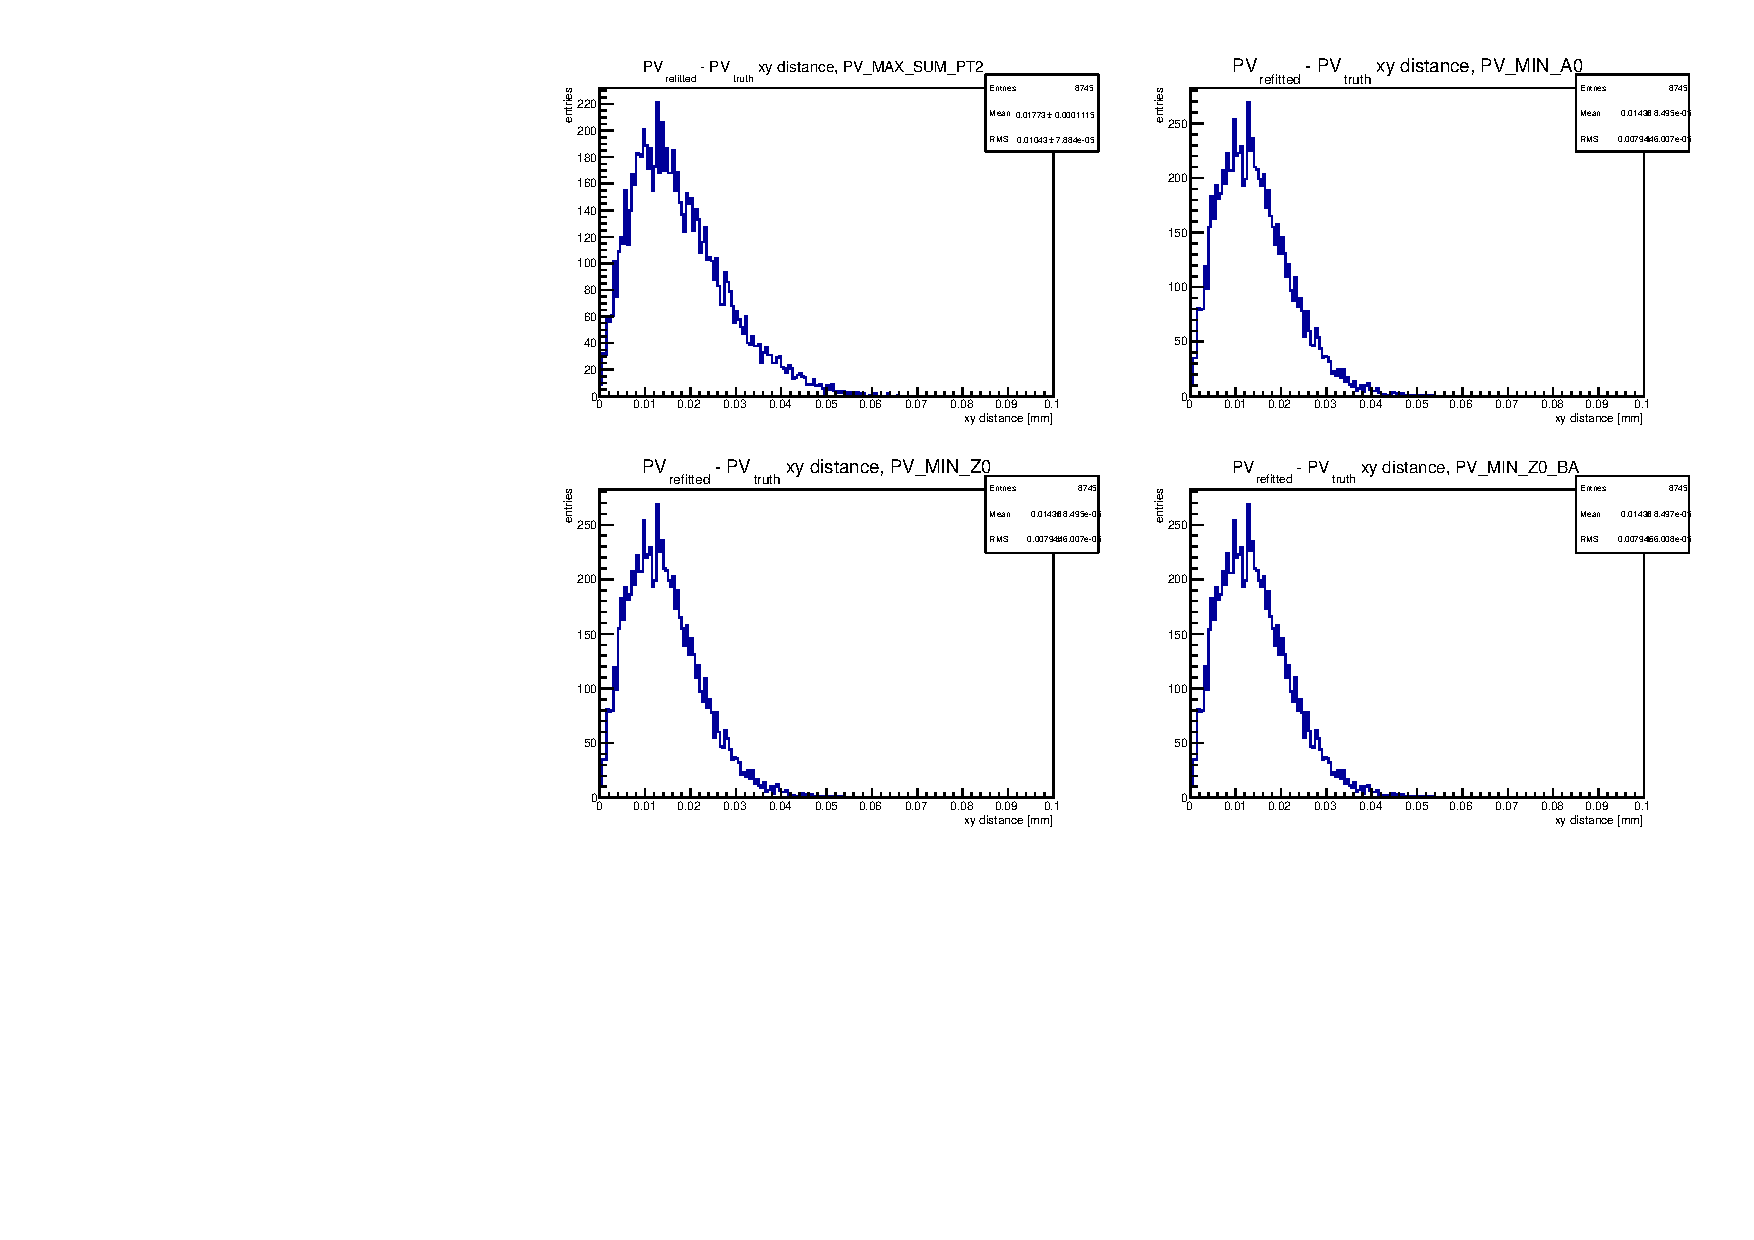
\includegraphics[width=15cm]{figures/InternalNote_Preselection/ref_xy_distance.pdf}
  \caption{xy distance between selected PV and truth PV for the four approaches.}
  \label{fig:PVSVass_xydist}
\end{figure}

\begin{figure}[h]
  \centering
  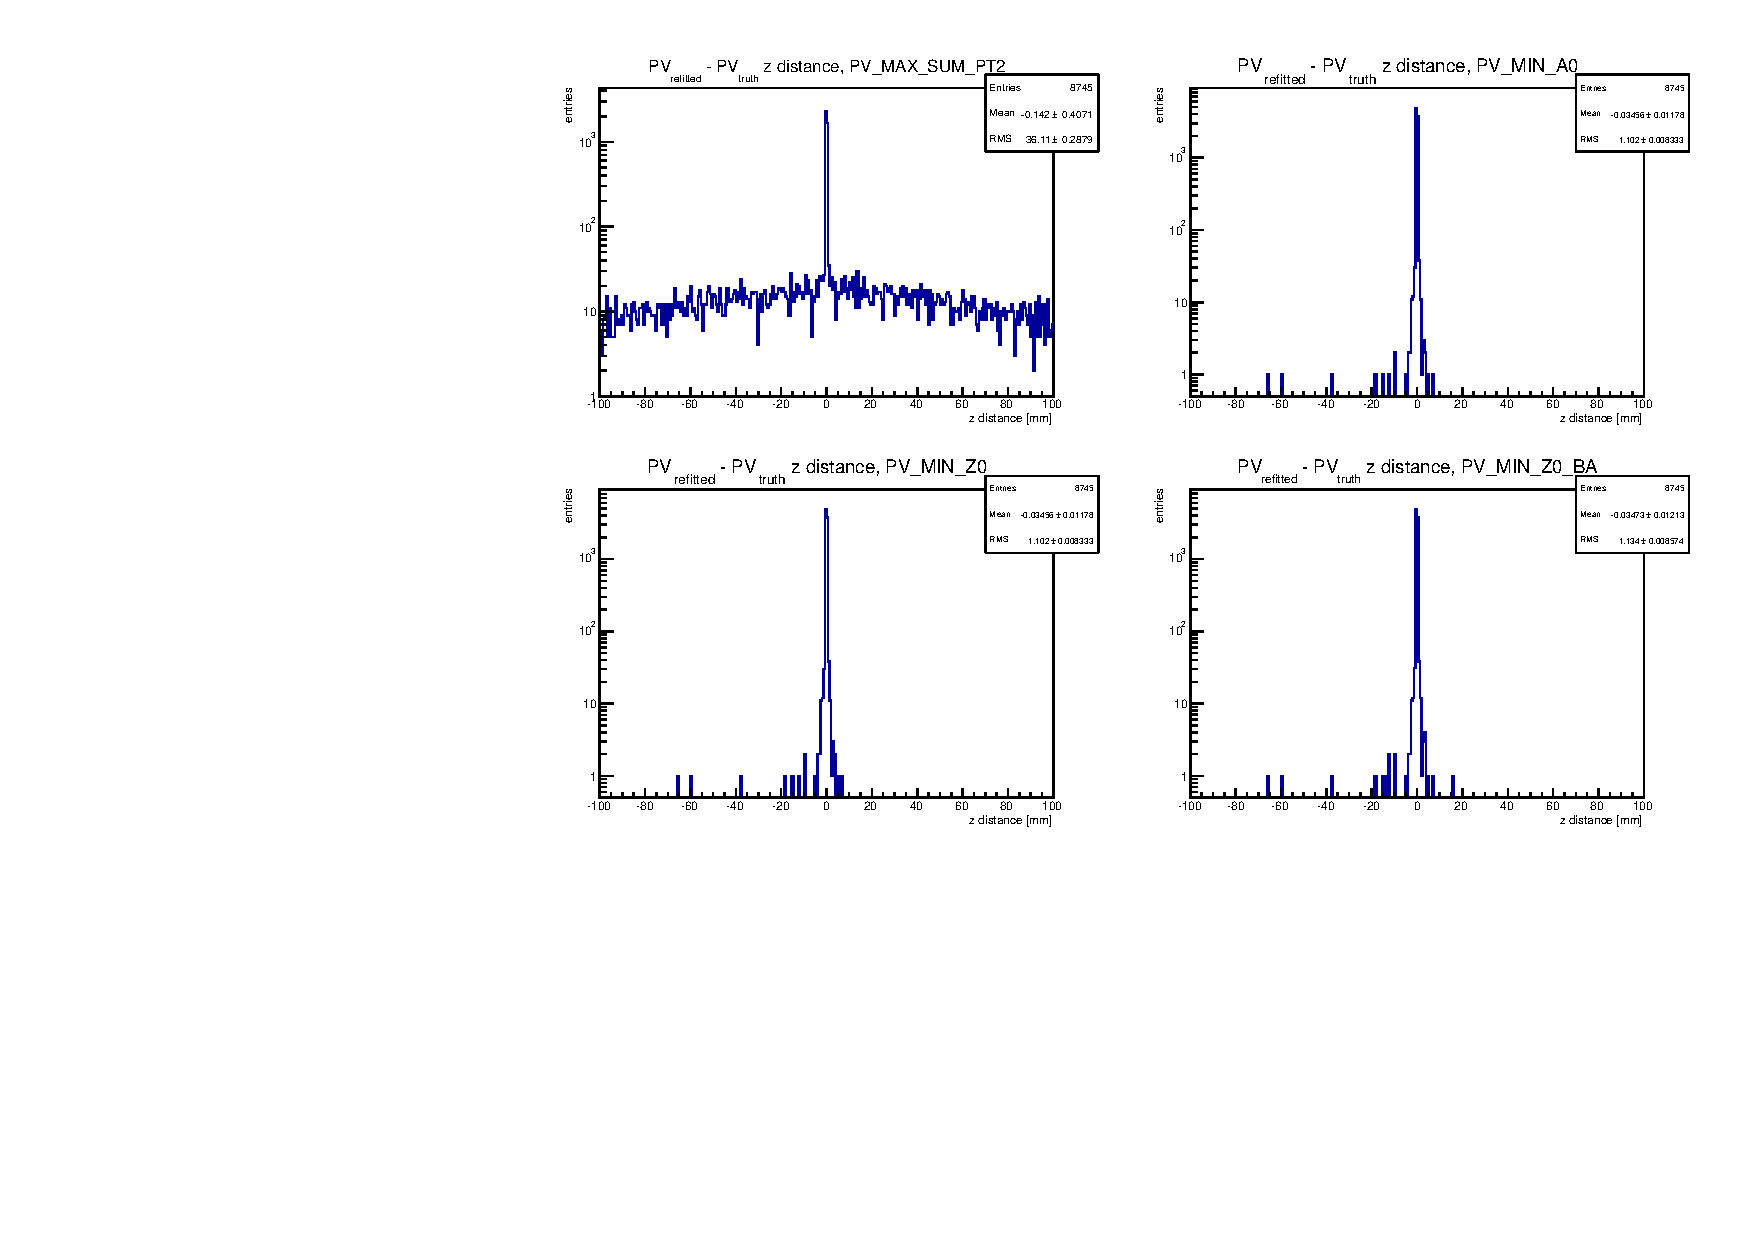
\includegraphics[width=15cm]{figures/InternalNote_Preselection/z_ref_distance_wide.pdf}
  \caption{z distance between selected PV and truth PV for the four approaches.}
  \label{fig:PVSVass_zdist}
\end{figure}

\begin{figure}[h]
  \centering
  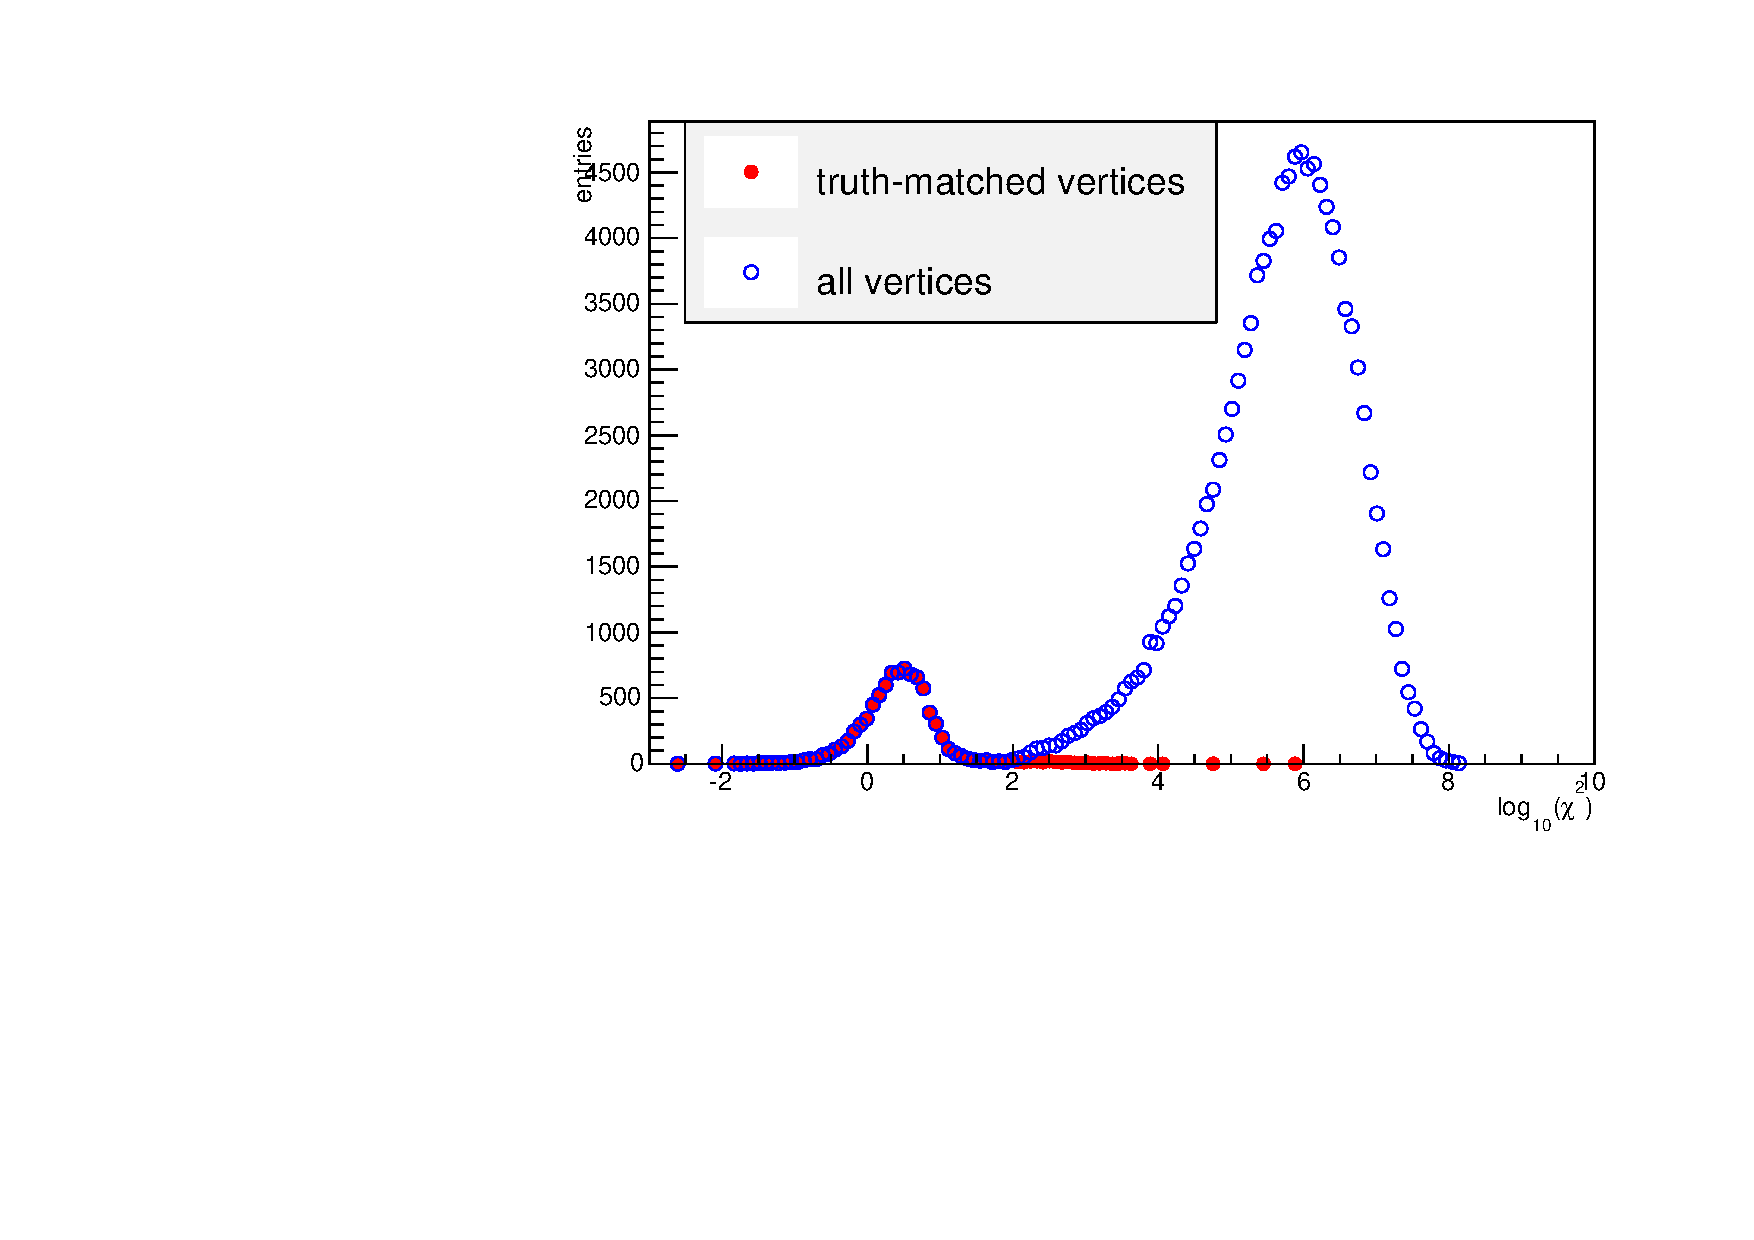
\includegraphics[width=15cm]{figures/InternalNote_Preselection/chi2DistAndMatched.pdf}
  \caption{$\chi^2$ of all the PVs (blue points) and the distribution of the $\chi^2$ of the “truth-matched” PVs.}
  \label{fig:Chi2DistAndMatched}
\end{figure}

\begin{figure}[h]
  \centering
  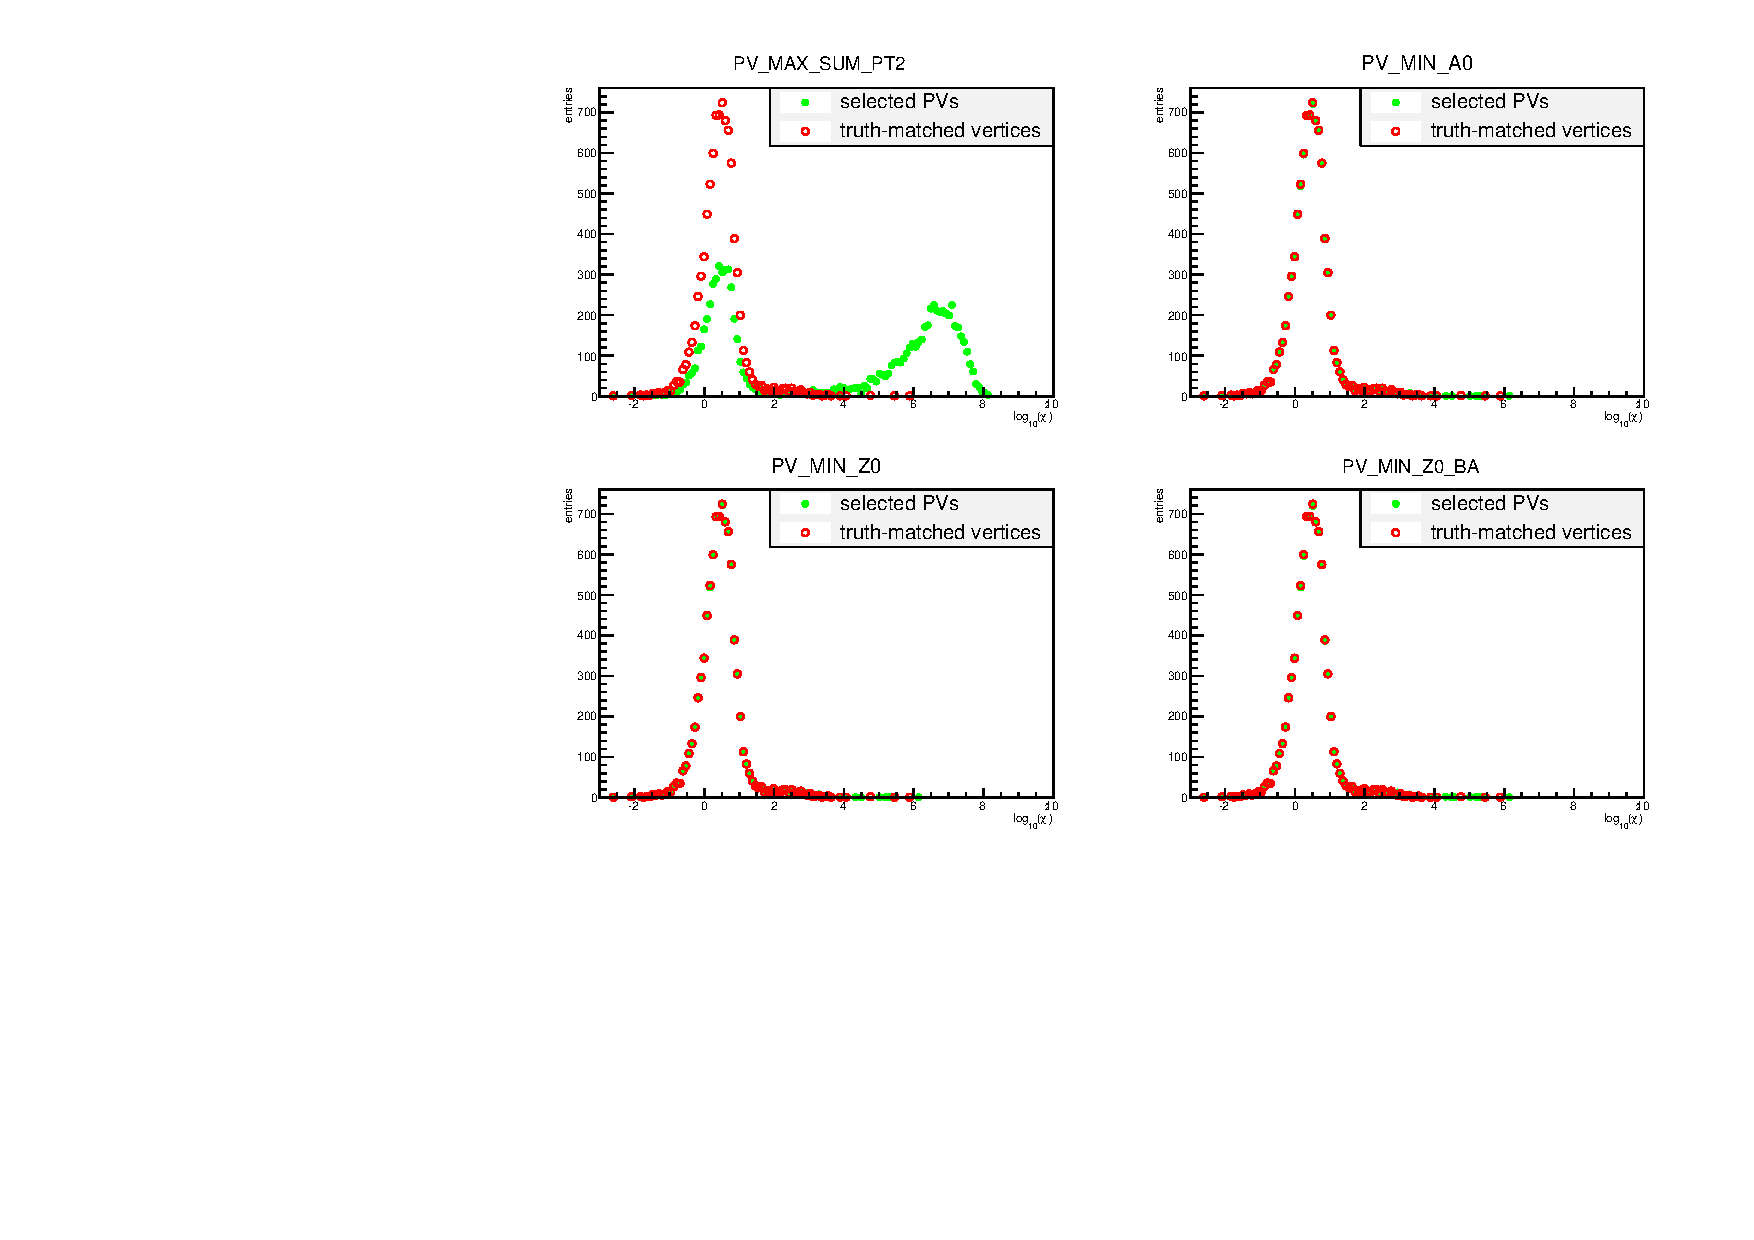
\includegraphics[width=15cm]{figures/InternalNote_Preselection/selectedChi2AndMatched.pdf}
  \caption{$\chi^2$ distribution of the chosen PVs using the 4 approaches (green distributions) superimposed to the truth-matched distribution (red).}
  \label{fig:selectedChi2AndMatched}
\end{figure}

\begin{figure}[h]
  \centering
  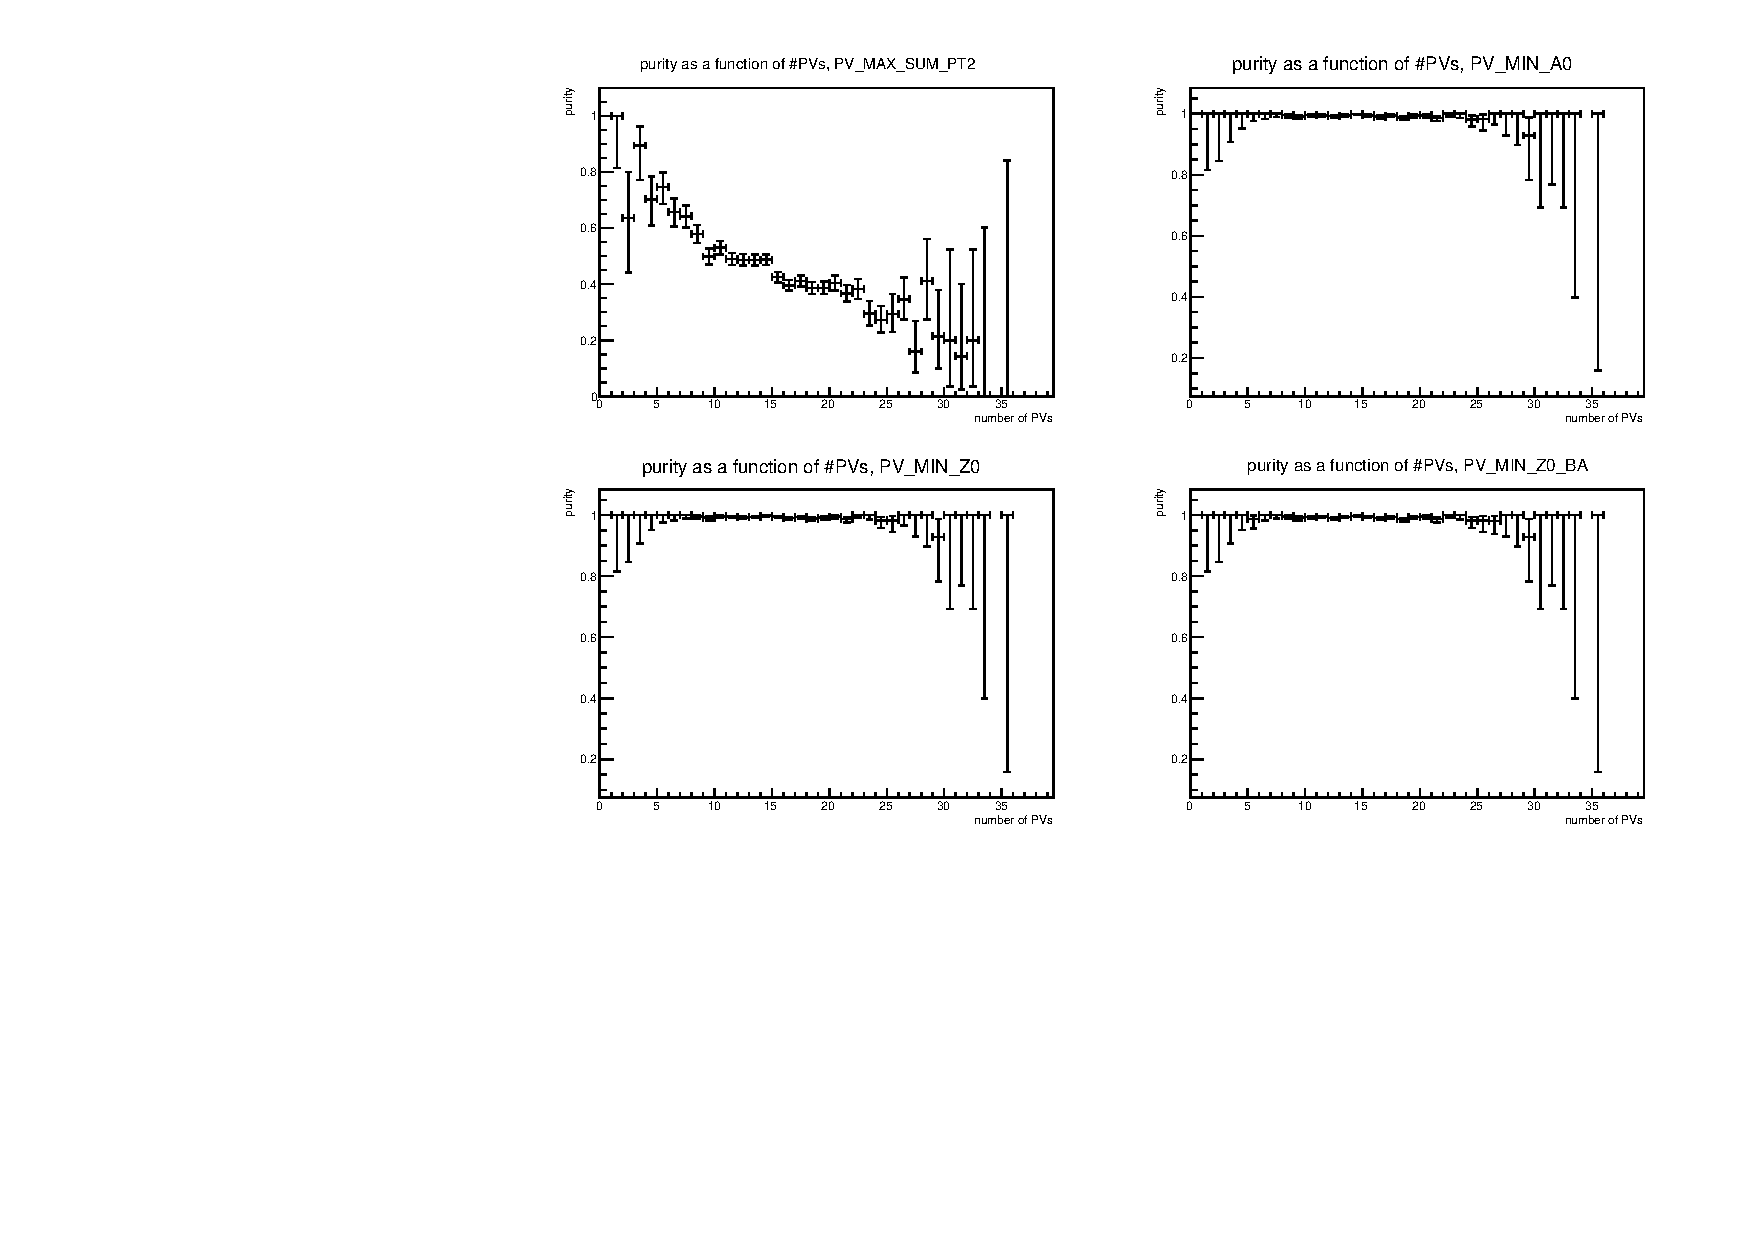
\includegraphics[width=15cm]{figures/InternalNote_Preselection/purityFuncNPV.pdf}
  \caption{purity as a function of number of reconstructed PVs for the four approaches.}
  \label{fig:purityFuncNPV}
\end{figure}



\clearpage

%% trigger studies
\section{Trigger}
\label{sec:Trigger}

In 2015-16 the main low \pt di-muon triggers were:
\begin{itemize}
\item {\it 2mu4} prescaled (2015) or not active (2016)
\item {\it mu6\_2mu4} prescaled during 2016, $\sim 82\%$ efficient w.r.t. 2mu4
\item {\it 2mu6} unprescaled, $\sim 35\%$ efficient w.r.t. 2mu4
\end{itemize}
The collected luminosity of each trigger per year are shown in table~\ref{table:collectedLumi}.
\begin{table}[h]
  \begin{center}
    \begin{tabular}{| c | c | c |}
      \hline
          &   2015  &  2016 \\  \hline
      2mu4 &  3.17 $\ifb$  & 0 $\ifb$ \\ \hline
      mu6mu4 & 3.93  $\ifb$  & 37.13 $\ifb$ \\ \hline
      2mu6 &  3.93  $\ifb$ & 26.03 $\ifb$ \\ \hline
   \end{tabular}
    \caption{Collected luminosity in 2015 and 2016.}
    \label{table:collectedLumi}
  \end{center}
\end{table}
%decide which triggers we want, possibilities
%2mu4+mu6mu4+2mu6  
%mu6mu4+2mu6
%mu6mu4 only GOOD

%some numbers
%total collected lumi     2015: 3.93 (2mu4 3.17)       2016:  37.13         mu6mu4 2016: 26.03
%2mu6+mu6mu4 = 28.5
%mu6mu4 = 24.6
%2mu4 addition would increase the 2mu6+mu6mu4 of a factor $\sim1%$

We can compare the available collected luminosity provided by the different triggers by calculating their effective collected luminosity, the total luminosity we would need to have the same amount of statistcs using 2mu4 as main trigger.
\begin{itemize}
\item consider mu6mu4 only would get an effective collected luminosity of 24.6 $\ifb$
\item consider the combination of mu6mu4 and 2mu6 would get an effective collected luminosity of 28.5 $\ifb$
\item 2mu4 addition would increase the 2mu6+mu6mu4 statistics of a factor $\sim 1 \%$
\end{itemize}
The prescaled trigger mu6mu4 provides the bulk of the statistics, which is $\sim 85 \%$ of total. The addition of 2mu6 would allow to use basically the full dataset but would also increase the complexity of the analysis, given the tight schedule, this round of the analysis will use mu6mu4 only.
%after that, talk about HLT-> _lxy0 and delayed stuff
%I have to say that L1_MU6_MU4 is always the same, but at HLT it changes, for 2015 HLT_mu6_mu4_bBmumu, for 2016 HLT_mu6_mu4_bBmumu_Lxy0 until some points and then HLT_mu6_mu4_bBmumu_Lxy0_delayed
%for the B+ don't really know
\add{still have to add the description of the different HLT algorithms (Lxy0, dalayed)}\\


In order compare the available statistics for this analysis with respect to the previous version, 
three main ingredients are needed.
\begin{enumerate}
\item \textbf{B production cross section with respect to Run-1}, due to the Run-2 
increased center of mass energy a value $\sim 1.7$ times higher is expected, 
according to studies performed using \yel[to be added in file bib]{FONLL ....}. %~\cite{FONLL}}.
\item \textbf{The efficiency of the dimuon triggers available in Run-2 with respect to the Run-1 triggers},  
already shown in this section.
\item \textbf{The collected luminosity for the selected trigger in Run-2}, an integrated luminosity 
of $\approx 40\ifb$ has been collected during the 2015 and 2016 data-taking period.
\end{enumerate}
The same signal over background ratio as the analysis performed on the Run-1 dataset is assumed for this study.\\
With the three ingredients listed above and the previous assumptions we estimate the expected 
statistics available for the 2015-16 dataset by scaling the Run-1 analysis 
statistics. This yields an estimated 2-fold increase with respect to Run-1 statistics.




\clearpage

%% cut flow
\section{CutFlow}
\label{sec:CutFlow}

\clearpage

%% fake rates
\section{Studies on muon fake rates}
\label{sec:MuonFakes}
%\newcommand{\quote}[1]{``#1''}
%quick introduction (mostly from Run1 int note)
One of the most problematic backgrounds in this study is represented
by the charmless two-body $B$ decays referred to as $B \to hh^\prime$,
$h$ being a charged $K$ or $\pi$. This background is topologically
identical to, and peaks under, the signal. 
The only handle we can exploit is the muon identification
capability of the ATLAS detector. For these decays to feed into
our events, the charged $K$ or $\pi$ has to be misidentified as a
muon. \\
In the previous analysis~\cite{Alpigiani:1756291} a dedicated analysis was carried out in order to reduce the fake rate thus reducing the contamination
from these background events. The misidentification fraction was found to be respectively 0.00076 
and 0.00101 for negative and positive $K$, and 0.00044 and 0.00042 for
 negative and positive $\pi$. The average misidentification fraction was $0.00067 \pm 0.00001$, for a muon efficiency of $95\%$.\\
Some of the variables used in the BDT of the previous analysis are now used in the muon quality definition, 
therefore we decide to check the misidentification fraction for the different muon qualities.\\


The study of fake muons has been performed on two MC samples of signal
(\Bsmumu) and charmless two-body decays ($B \to hh^\prime$). %, with $h$, $h^\prime$=$K$ or $\pi$).
These samples have been produced with full GEANT simulation in order
to accurately describe the hadrons after they leave the Inner Detector. % the calorimeter response.
The preselection described in Section~\ref{sec:CandidatesPreselection}
is applied to the events entering this study (except for the muon quality requirement). A di-muon trigger request
 (mu6mu4) is applied to the \Bsmumu sample, while events containing preselected hadrons 
from $B\to hh^\prime$ that are misidentified as muons
are required to satisfy a single muon trigger ({\it{mu4}}). Once an event has 
passed the preselction, the two final state particles are considered separetely.\\
Table~\ref{table:misidentfraction} show the misidentification fraction and the muon efficiency for the different muon qualities available and for the previous analysis.
\begin{table}[h]
  \begin{center}
    \begin{tabular}{| c | c | c | c | c | c |}
      \hline
      &run1 presel + trigger match&run1 fake-BDT&loose muons&medium muons&tight muons\\ \hline
      total&0.00181&0.00067&0.00221&0.00221&0.00109\\ \hline
      total +&&&0.00229&0.00228&0.00114\\ \hline
      total -&&&0.00214&0.00213&0.00105\\ \hline
      total $\pi$&&0.0004&0.0018&0.0018&0.00101\\ \hline
      total K&&0.0009&0.00264&0.00263&0.00118\\ \hline
      $\pi^+$&0.00121&0.00042&0.00177&0.00177&0.00101\\ \hline
      $\pi^-$&0.00116&0.00044&0.00183&0.00182&0.00101\\ \hline
      $K^+$&0.00263&0.00101&0.00281&0.00281&0.00127\\ \hline
      $K^-$&0.00207&0.00076&0.00246&0.00245&0.00109\\ \hline
      &&&&&\\ \hline
      $\mu$ eff&&0.95&0.997&0.996&0.935\\ \hline
      $\mu^+$ eff&&&0.997&0.996&0.935\\ \hline
      $\mu^-$ eff&&&0.997&0.997&0.935\\ \hline
    \end{tabular}
    \caption{misidentification fraction and muon efficiency for the three 
      available muon qualities (loose, medium and tight) and, for comparison, 
      from the previous analysis~\cite{Alpigiani:1756291}, for different edmixtures of positive and negative $\pi$ and $K$.
      Misidentification fraction is calculated as the ratio of the number 
      of hadrons after all selections and the quality requirements divided 
      by the total number of hadrons that pass all selections. Muons 
      efficiency is defined as the number of muons that pass all selections and the quality requirements divided
      by the total number of muons that pass all selections.}
    \label{table:misidentfraction}  
  \end{center}
\end{table}
Tight muons have a comparable misidentification fraction and muon efficiency to the Run1 BDT; their usage would 
imply an increase of about $\sim \times 1.6$ in the number of fakes than using a Run1-like BDT, 
for about the same muon efficiency.\\
In order to understand the effect of the tight muons usage, we compared the effect of a Run1-like BDT and the tight muons in the analysis.\\
Knowing the available statistics before and after the fake-BDT application in previous 
analysis~\cite{Alpigiani:1756291} and the muon efficiency and fake-rate, we computed the 
Run1 background composition in terms of fake and real muons; applying the properties of tight muons we can estimate the effect 
tight muons would have had on the Run1 analysis.
Tables~\ref{table:bkgInRun1_BDTandTightMu} and ~\ref{table:sigInRun1_BDTandTightMu} show the amount 
of statistics for the different components of the likelihood used in the fit for the signal yield extraction 
and the estimation of the statistics using tight muons. The combinatorial background doesn't increase significantly, 
the SS-SV (ans semileptonic) background increases of a factor $\sim \times 1.1$ and the paking background increases 
of a factor $\sim \times 2.6$. Signal reduction due to lower muon efficiency is almost negligibe.\\
\begin{table}[h]
  \begin{center}
    \begin{tabular}{| c | c | c | c | c |}
      \hline
       & comb bkg run1 & comb bkg tight mu & SS-SV bkg run 1 & SS-SV bkg tight mu\\  \hline
      bin 1 & 1455.3 & 1460.7 & 205.5 & 229.0\\  \hline
      bin 2 & 110.5 & 110.9 & 105.6 & 117.7\\  \hline
      bin 3 & 11.6 & 11.6 & 51.2 & 57.1\\  \hline
   \end{tabular}
    \caption{breakdown of the background contributions in the Run1 likelihood after the BDT application. 
    Columns labelled tight mu show the estimated statistcs we would have gotten using tight muons instead of the BDT.}
    \label{table:bkgInRun1_BDTandTightMu}
  \end{center}
\end{table}
\begin{table}[h]
  \begin{center}
    \begin{tabular}{| c | c | c |}
      \hline
       & run 1 & run 1 with tight mu  \\ \hline
      nBs (SM expected) & 41 & 39.7 \\ \hline
      nBd (SM expected) & 5 & 4.8 \\ \hline
      peaking bkg & 1 & 2.6 \\ \hline
    \end{tabular}
    \caption{Breakdown of the expected signal and peaking background contributions in the Run1 likelaihood after the BDT application. 
    Columns labelled tight mu show the estimated statistcs we would have gotten using tight muons instead of the BDT.}
    \label{table:sigInRun1_BDTandTightMu}
  \end{center}
\end{table}
In order to asses the impact of tight muons usage on the analysis performance a set of toy-MC 
based on the Run1 analysis likelihood with the available statistics modified according 
to the estimation of the available stastics in this analysis performed in section~\ref{sec:Trigger} 
has been run, varying the number of events associated to the different background and signal models according to the usage of tight muons 
or a Run1-like BDT. Table~\ref{table:tightMuAndBDTRMS} shows the root mean square of the distribution 
of the fitted number of $B_s$ and $B_d$ events. No significant effect on analysis sensitivity is 
visible for $B_s$, while a $\sim 1\%$ broader RMS is visible on $B_d$ count.\\
Given the negligible difference due to the usage of tight muons instead of a Run1-like BDT for fake 
muons reduction, we decide to use tight muons instead of developing and ad-hoc BDT for this analysis.
\begin{table}[h]
  \begin{center}
    \begin{tabular}{| c | c | c || c | c |}
      \hline
      &Run1 fake-BDT&Run1 tight muons&Run2 fake-BDT&Run2 tight muons\\ \hline
      RMS nBs&15.20 $\pm$ 0.01&15.16 $\pm$ 0.01&21.260 $\pm$ 0.015&21.260 $\pm$ 0.015\\ \hline
      RMS nBd&13.88 $\pm$ 0.01&13.96 $\pm$ 0.01&18.850 $\pm$ 0.015&19.130 $\pm$ 0.015\\ \hline
    \end{tabular}
    \caption{RMS of distributions of number of fitted $B_s$ and $B_d$ events in toy-MC study. The columns labelled Run1 
      refer to the statistcs available in the previous analysis, modified for the usage of tight muons in case of the 
    second column. Columns labelled Run2 refer to the estimation of the statistics available for this analysis performed in section~\ref{sec:Trigger}.}
    \label{table:tightMuAndBDTRMS}
  \end{center}
\end{table}
\clearpage

% Background Modeling
\usetikzlibrary{decorations.pathmorphing}
\usetikzlibrary{arrows.meta}
\tikzset{snake it/.style={decorate, decoration=snake}}

%----------------------------------------
%Commands
%----------------------------------------
\newcommand{\textblue}[1]{ \color{blue}#1\color{black} }
\newcommand{\textred}[1]{ \color{red}#1\color{black} }
\newcommand{\textgreen}[1]{ \color{red}#1\color{black} }
%----------------------------------------
%Analysis
%----------------------------------------
\newcommand{\bsmumu}{B_{s}^{0}\rightarrow \mu^{+}\mu^{-}}
\newcommand{\bpjpsik}{B^{+}\rightarrow J/\psi+K^{+}}
\newcommand{\bsjpsiphi}{B_{s}^{0}\rightarrow J/\psi + \phi}

\newcommand{\bbmumux}{b\bar{b}\rightarrow\mu^+\mu^-+X}
\newcommand{\bbjpsix}{b\bar{b}\rightarrow J/\psi+X}
%----------------------------------------
%Useful to make diagrams
%----------------------------------------
\newcommand\tikzwidth{3}
\newcommand\tikzwidthwide{3}
\newcommand\tikzheight{0.25}
\newcommand\tikzdec{0.9}

\usetikzlibrary{shapes.geometric, arrows}
\tikzstyle{Round-rectangle-trans} = [rectangle, rounded corners, minimum width=\tikzwidth cm, minimum height=\tikzheight cm,text centered, text width=\tikzwidth cm, draw=white, fill=white!30]
\tikzstyle{Round-rectangle-white} = [rectangle, rounded corners, minimum width=\tikzwidth cm, minimum height=\tikzheight cm,text centered, text width=\tikzwidth cm, draw=black, fill=white!30]
\tikzstyle{Round-rectangle-blue} = [rectangle, rounded corners, minimum width=\tikzwidth cm, minimum height=\tikzheight cm,text centered, text width=\tikzwidth cm, draw=black, fill=blue!30]
\tikzstyle{Round-rectangle-green} = [rectangle, rounded corners, minimum width=\tikzwidth cm, minimum height=\tikzheight cm,text centered, text width=\tikzwidth cm, draw=black, fill=green!50]
\tikzstyle{Round-rectangle-red} = [rectangle, rounded corners, minimum width=\tikzwidth cm, minimum height=\tikzheight cm,text centered, text width=\tikzwidth cm, draw=black, fill=red!50]

\tikzstyle{Round-rectangle-trans-wide} = [rectangle, rounded corners, minimum width=\tikzwidthwide cm, minimum height=\tikzheight cm,text centered, text width=\tikzwidth cm, draw=white, fill=white!30]
\tikzstyle{Round-rectangle-white-wide} = [rectangle, rounded corners, minimum width=\tikzwidthwide cm, minimum height=\tikzheight cm,text centered, text width=\tikzwidth cm, draw=black, fill=white!30]
\tikzstyle{Round-rectangle-blue-wide} = [rectangle, rounded corners, minimum width=\tikzwidthwide cm, minimum height=\tikzheight cm,text centered, text width=\tikzwidth cm, draw=black, fill=blue!30]
\tikzstyle{Round-rectangle-green-wide} = [rectangle, rounded corners, minimum width=\tikzwidthwide cm, minimum height=\tikzheight cm,text centered, text width=\tikzwidth cm, draw=black, fill=green!50]
\tikzstyle{Round-rectangle-red-wide} = [rectangle, rounded corners, minimum width=\tikzwidthwide cm, minimum height=\tikzheight cm,text centered, text width=\tikzwidth cm, draw=black, fill=red!50]

\tikzstyle{rectangle-trans} = [rectangle, minimum width=\tikzwidth cm, minimum height=\tikzheight cm,text centered, text width=\tikzwidth cm, draw=white, fill=white!30]
\tikzstyle{rectangle-white} = [rectangle, minimum width=\tikzwidth cm, minimum height=\tikzheight cm,text centered, text width=\tikzwidth cm, draw=black, fill=white!30]
\tikzstyle{rectangle-blue} = [rectangle, minimum width=\tikzwidth cm, minimum height=\tikzheight cm,text centered, text width=\tikzwidth cm, draw=black, fill=blue!30]
\tikzstyle{rectangle-green} = [rectangle, minimum width=\tikzwidth cm, minimum height=\tikzheight cm,text centered, text width=\tikzwidth cm, draw=black, fill=green!50]
\tikzstyle{rectangle-red} = [rectangle, minimum width=\tikzwidth cm, minimum height=\tikzheight cm,text centered, text width=\tikzwidth cm, draw=black, fill=red!50]

\tikzstyle{rectangle-trans-wide} = [rectangle, minimum width=\tikzwidthwide cm, minimum height=\tikzheight cm,text centered, text width=\tikzwidth cm, draw=white, fill=white!30]
\tikzstyle{rectangle-white-wide} = [rectangle, minimum width=\tikzwidthwide cm, minimum height=\tikzheight cm,text centered, text width=\tikzwidth cm, draw=black, fill=white!30]
\tikzstyle{rectangle-blue-wide} = [rectangle, minimum width=\tikzwidthwide cm, minimum height=\tikzheight cm,text centered, text width=\tikzwidth cm, draw=black, fill=blue!30]
\tikzstyle{rectangle-green-wide} = [rectangle, minimum width=\tikzwidthwide cm, minimum height=\tikzheight cm,text centered, text width=\tikzwidth cm, draw=black, fill=green!50]
\tikzstyle{rectangle-red-wide} = [rectangle, minimum width=\tikzwidthwide cm, minimum height=\tikzheight cm,text centered, text width=\tikzwidth cm, draw=black, fill=red!50]

\tikzstyle{startstop} = [rectangle, rounded corners, minimum width=\tikzwidth cm, minimum height=\tikzheight cm,text centered, text width=\tikzwidth cm, draw=black, fill=red!30]
\tikzstyle{io} = [trapezium, trapezium left angle=70, trapezium right angle=110, minimum width=\tikzwidth cm, minimum height=\tikzheight cm, text centered, draw=black, fill=blue!30]
\tikzstyle{process} = [rectangle, minimum width=\tikzwidth cm, minimum height=\tikzheight cm, text centered, text width=\tikzwidth cm, draw=black, fill=orange!30]
\tikzstyle{decision} = [circle, minimum width=\tikzdec cm, minimum height=\tikzdec cm, text centered, text width=\tikzdec cm, draw=black, fill=green!30]
\tikzstyle{arrow} = [thick,->,>=stealth]
%----------------------------------------



\section{Background Modeling}
\label{sec:BackgroundModeling}

\subsection{Non-resonant Background}
\label{sub:sec:continuum}


The measurement of the rare decay of $B$ mesons into muon pairs
requires the rejection of a very large combinatorial background.
After the preliminary and additional selection, the amount of combinatorial
background is at the level of \yel[numbers t.b.u.]{$\approx$140~k events per 100~MeV} interval
in the muon pair invariant mass (this is shown in the context of the
normalisation study for the signal fit in Figure~\ref{fig:sbvars}).
This figure should be compared to $\approx$20 events/100~MeV expected
at the peak of the \Bs\ signal (section~\ref{sub:sec:bkg-normalisation-fit}).  

To have a statistically meaningful sample of this combinatorial background,
a very large number of events needs to be generated
(one of the largest MC production performed so far by ATLAS for a single analysis), 
thus specific procedures have been used in order to reduce the event generation
time, as discussed below.  
The MC sample was generated inclusively to provide a realistic composition of muons
from different sources, including non combinatorial sources of muon pairs. 
On the other hand, because of uncertainties in cross sections and branching ratios, 
as well as for those related to the generation procedures, 
%(repeated hadronisation and repeated decays)
no attempt is made to use the MC to draw quantitative conclusions
on the amount in which each type of background is present in real data.
For that purpose, events collected in the sidebands are used.
As shown in section~\ref{sub:sec:bkg-normalisation-fit}, after the background
reduction developed on MC is applied, the remaining background in real data is
sufficiently low and separated in its different components to be used for an
effective interpolation in the signal region. 

In order to optimise the production speed, {\em repeated hadronisation} and {\em repeated decay}
procedures were used for the inclusive MC, in order to reduce the typical generation time
from a several minutes per event to only about 40 seconds. 

Repeated hadronisation, performed in \Pythia, was applied with 10 repetitions. 
This is technically implemented by means of PythiaB
package~\cite{PythiaB} and had already been widely tested and used for various MC
production in $B$ physics. This procedure scarcely affects the characteristics of
the generated samples. 

The next step, decays of the unstable particles, has been done differently with respect to Run 1,
since the procedure employed back then effectively enhanced the acceptance at lower \pT, which
required a correction. Currently, each hadronised event is cloned fixed number of times (200) by \Pythia~and each cloned event
decays independently. In the next step a generator level filtering (e.g. cuts on muons transverse momenta) is applied, 
and all cloned events which pass it are stored in the resulting sample. 
This approach allows events with identical b hadron kinematics if more than one of those 200 
clones produce a muon pair, which passes the filter. 
However, this approach does not introduce the kinematic bias we had in Run 1. With
\Pythia (unlike \textsc{EvtGen} used in Run 1) we have less up-to-date decay tables 
and no angular decay models. However the last 
effect we found to be negligible for the decays we require - with two muons in the final state.
The residual descrepancies in kinematic of B-candidates and multiplicity of tracks in the vicinity
of reconsructed di-muon vertices are corrected on data.

If only standard cuts are applied to the
muons and loose cuts are applied to the muon pair, the MC sample is dominated
by opposite side combinatorial background (about \yel[numbers t.b.u.]{20~M events in the mass interval
4.8-5.9~GeV, with 50~k} events of different nature). When a multivariate selection
aiming at the rejection of combinatorial background is applied  (as discussed
in Sec~\ref{sec:contBDT}), the relevance of the additional contribution becomes
more evident (e.g., for a selection aiming at \yel[numbers t.b.u.]{60~\%  (20~\%) efficiency} for the signal
\Bsmumu, opposite side events account for about \yel[numbers t.b.u.]{95 \% (40 \%)} of the muon pairs
in the mass interval 4.8--5.9 GeV). The additional events are mainly due to
same-side combinatorial  background from $B$ meson decays, and also to exclusive
decays such as $\Bc^+ \to \Jpsi \, \mu^+ \nu$, $B \to K \, \mu^+\mu^- (\gamma)$,
$\Bs \to \mu^+ \mu^-(\gamma)$  (\yel[numbers t.b.u.]{XXX} signal events are present in the four-corner
MC sample).


Because of the uncertainties discussed above, information extracted from the relative
normalisation of the different types of backgrounds and of the signal events present
in the inclusive sample are not used in any part of the analysis.
On the other hand, the samples of data obtained from MC have shown
remarkable consistency with real data collected in the side-bands of the
signal region, in their dependence on the di-muon invariant mass and on
the BDT classifier.
It is also remarkable that the simulation shows that exclusive
semileptonic decays $\Bz \to \pi\mu\nu$, $\Bs \to K\mu\nu$, with the hadron being
misidentified as muon, provide a background of negligible size
compared to same-side cascade events, or \Bc\ background. 


\subsection{Background Classification}
\label{sub:sec:bkgclass}
\graphicspath{ {figures/InternalNote_BackgroundModeling/} }

The three processes of interest are $\bsmumu$, $\bpjpsik$ and $\bsjpsiphi$. In order to estimate the different
background contributions to each of them, the MC in table \ref{table:inclusive_mc} is used.

\begin{table}[h!]
    \centering
    \begin{tabular}{|l | c | r | l|} 
	\hline
	Process & DSID & Events & Generator\\ [0.5ex] 
	\hline
	\hline
	$\bbmumux$ & 300307 & 600M & PYTHIA + PHOTOS\\ 
	$\bbjpsix$ & 300203 & 10M & PYTHIA\\ [1ex] 
	\hline
    \end{tabular}
    \caption{Inclusive background samples used to find background contributions.}
    \label{table:inclusive_mc}
\end{table}

The same reconstruction algorithms that would be applied to the three exclusive MC samples
are applied to the inclusive samples. From this, containers with candidates misidentified as
$B_{s}^{0}$ and $B^{+}$ are created. The reconstructed objects, both muons and tracks can be 
matched to the corresponding truth objects. In this way, one can create a string representing the
decay process responsible for the reconstructed $B$ candidate. Figure \ref{fig:reco_truth_assoc_comb}
shows this, in this case, given that the upper most truth $B$ candidate does not exist (there are two,
each associated to a $b$ quark), this reconstructed $B_{s}^{0}$ would be combinatorial background.

\begin{figure}[ht]
    \centering
    \subfloat[Combinatorial background]
    {
	\begin{tikzpicture}[thick, scale = 1]
	    \draw[red,-{Latex[length=1.5mm]}](0.2,4) node[above]{$b$} (0.2,4)--(1,1) node[right]{$\mu^+$};
	    \draw[red,-{Latex[length=1.5mm]}](-0.2,4) node[above]{$\bar{b}$} (-0.2,4)--(-1,1) node[left]{$\mu^-$};

	    \draw[red,-{Latex[length=1.5mm]}] (0.2,4)--(3,2) node[below]{$X$};
	    \draw[red,-{Latex[length=1.5mm]}] (-0.2,4)--(-3,2) node[below]{$Y$};

	    \path [draw=black,snake it] (-4,0) -- (4,0);
	    \draw[dashed] (1,1)--(1,-1);
	    \draw[dashed] (-1,1)--(-1,-1);


	    \draw[blue,-{Latex[length=1.5mm]}] (1,-1)--(2,-3) node[below]{$\mu^+$};
	    \draw[blue,-{Latex[length=1.5mm]}] (-1,-1)--(-2,-3) node[below]{$\mu^-$};

	    \draw(-3,-2)node[fill=white, text=blue]{Reconstructed};
	    \draw(-3,+1)node[fill=white, text=red]{Truth};
	\end{tikzpicture}
	\label{fig:reco_truth_assoc_comb}
    }
    \subfloat[Partially reconstructed decay]
    {
	\begin{tikzpicture}[thick, scale = 1]
	    \draw[red,-{Latex[length=1.5mm]}](0,4)                          (0,4)--(-1,2) node[left]{$K^*$};
	    \draw[red,-{Latex[length=1.5mm]}] (-1,2)--(-0.5,1) node[right]{$K^+$};
	    \draw[red,-{Latex[length=1.5mm]}] (-1,2)--(-1.5,1) node[below]{$\pi^-$};

	    \draw[red,-{Latex[length=1.5mm]}](0,4) node[above]{$B_{d}^{0}$} (0,4)--(1,2) node[right]{$J/\psi$};
	    \draw[red,-{Latex[length=1.5mm]}] (1,2)--(1.5,1) node[right]{$\mu^+$};
	    \draw[red,-{Latex[length=1.5mm]}] (1,2)--(0.5,1) node[right]{$\mu^-$};

	    \path [draw=black,snake it] (-4,0) -- (4,0);

	    \draw[dashed] (1.5,1)--(1.5,-1);
	    \draw[dashed] (0.5,1)--(0.5,-1);
	    \draw[dashed] (-0.5,1)--(-0.5,-1);


	    \draw[blue,-{Latex[length=1.5mm]}] (1.5,-1)--(1.5,-3) node[below]{$\mu^+$};
	    \draw[blue,-{Latex[length=1.5mm]}] (0.5,-1)--(0.5,-3) node[below]{$\mu^-$};

	    \draw[blue,-{Latex[length=1.5mm]}] (-0.5,-1)--(-1,-3) node[below]{$K^+$};


	    \draw(-3,-2)node[fill=white, text=blue]{Reconstructed};
	    \draw(-3,+1)node[fill=white, text=red]{Truth};
	\end{tikzpicture}
	\label{fig:reco_truth_assoc_partial}
    }
    \caption{Both diagrams represent a reconstructed $B_{s}^0$ or $B^+$, which in reality are
    combinatorial background or a partially reconstructed decay.}
    \label{fig:reco_truth_assoc}
\end{figure}

On the other hand, figure \ref{fig:reco_truth_assoc_partial} shows a reconstructed $B^+$ candidate
originating from a partially reconstructed decay. In this case the decay string would be \textit{B0[K*0[pi-:K+]Jpsi[mu+:mu-]]}.\\

\subsubsection{Truth Matching}
Figures \ref{fig:reco_truth_assoc} show, as a dashed black line, the truth and reconstructed objects matching.
In order to match them one requires $\Delta R < 0.05$. Preliminary studies have shown that the optimal value for this
cone is $0.01$; but a larger radius should prevent us from loosing any truth candidate. In order to prevent truth objects that
are not associated with the reconstructed object, from entering the cone, we require:

\begin{equation}
    \left|1-\frac{p_T^{truth}}{p_T^{reco}}\right|<0.15
\end{equation}

Also, reconstructed muons are required to be matched to muons with the same charge. The kaons are required to be
matched with truth light hadrons, either mesons or baryons.

\subsubsection{Cumulative Decay Probability Distribution}
A natural question now would be, how many different events in the inclusive background survive the 
candidate selection and get reconstructed? Figure \ref{fig:bbjpsix_cutflow} shows the number of events and candidates
at each stage of the analysis, from the xAOD level until the ntuples.

\begin{figure}
    \centering
    \begin{tikzpicture}[node distance=3cm]
	\node (xAOD)  [Round-rectangle-blue, xshift=-3cm] {xAOD\\ 9.9E+06};

	\node (DxAOD) [Round-rectangle-blue, yshift=0.5cm, below of=xAOD] {DxAOD\\ 6.2E+06};
	\draw [arrow, draw=black] (xAOD) --node[] {} (DxAOD);

	\node (NTP_B2) [Round-rectangle-blue, xshift=-4cm, yshift=-0.5cm, below of=DxAOD] {1.6E+07 Candidates\\5.6E+06 Events};
	\node (TREE_B2) [Round-rectangle-blue, yshift=0cm, below of=NTP_B2] {1.7E+05 Combinatorial\\3.8E+06 Unmatched\\3.0E+06 Decays};
	\draw [arrow, draw=black] (NTP_B2) --node[text centered, sloped, above] {cuts} (TREE_B2);

	\node (NTP_B1) [Round-rectangle-blue, xshift=0cm, yshift=-0.5cm, below of=DxAOD] {1.5E+05 Candidates\\1.5E+05 Events};
	\node (TREE_B1) [Round-rectangle-blue, yshift=0cm, below of=NTP_B1] {1.1E+04 Combinatorial\\3.4E+03 Unmatched\\3.5E+03 Decays};
	\draw [arrow, draw=black] (NTP_B1) --node[text centered, sloped, above] {cuts} (TREE_B1);

	\node (NTP_B3) [Round-rectangle-blue, xshift=+4cm, yshift=-0.5cm, below of=DxAOD] {8.5E+06 Candidates\\2.7E+06 Events};
	\node (TREE_B3) [Round-rectangle-blue, yshift=0cm, below of=NTP_B3] {8.8E+04 Combinatorial\\2.6E+06 Unmatched\\7.9E+05 Decays};
	\draw [arrow, draw=black] (NTP_B3) --node[text centered, sloped, above] {cuts} (TREE_B3);

	\draw [arrow, draw=black] (DxAOD) --node[text centered, sloped, above] {$B_{s}\rightarrow\mu\mu$} (NTP_B1);
	\draw [arrow, draw=black] (DxAOD) --node[text centered, sloped, above] {$B^{+}\rightarrow J/\psi K^{+}$} (NTP_B2);
	\draw [arrow, draw=black] (DxAOD) --node[text centered, sloped, above] {$B_{s}\rightarrow J/\psi \phi$} (NTP_B3);
    \end{tikzpicture}
    \caption{Cutflow corresponding to $\bbjpsix$ sample.}
    \label{fig:bbjpsix_cutflow}
\end{figure}

The cuts used in the last level are:

\begin{itemize}
    \item \textbf{Muons:} Combined muons that pass MCP requirements and $|\eta|<2.5$, $p_{T}>4GeV$.
    \item \textbf{Kaons:} Must pass loose requirements and $|\eta|<2.5$, $p_{T}>1GeV$.
    \item \textbf{Candidates:} $|\eta|<2.5$, $p_{T}>8GeV$, $\chi^{2}<6$.
\end{itemize}

Another thing that we might want to know is the number of decays present in the samples. Figure 
\ref{fig:decay_multiplicity} shows the cumulative distribution of decays vs the decay index, where the most
common decays are put first. From this we can conclude that, as expected, the $\bbmumux$ sample
contains very few $\bsmumu$ candidates and mostly $\bpjpsik$ and $\bsjpsiphi$ candidates.
Two mass windows were used, the wide window contains much more decays than the narrow one.
This is because in the low end of the mass spectrum, partially reconstructed decays, like the one
in \ref{fig:reco_truth_assoc_partial}, accumulate. The narrow mass window removes all of them.
Another thing that the plot tells us is that there are many more background processes associated
to the $\bsjpsiphi$ candidates than to the $\bpjpsik$ candidates.

\begin{figure}[ht]
    \centering
    \subfloat[\scriptsize $B_{s}\rightarrow\mu\mu$.]
    {
	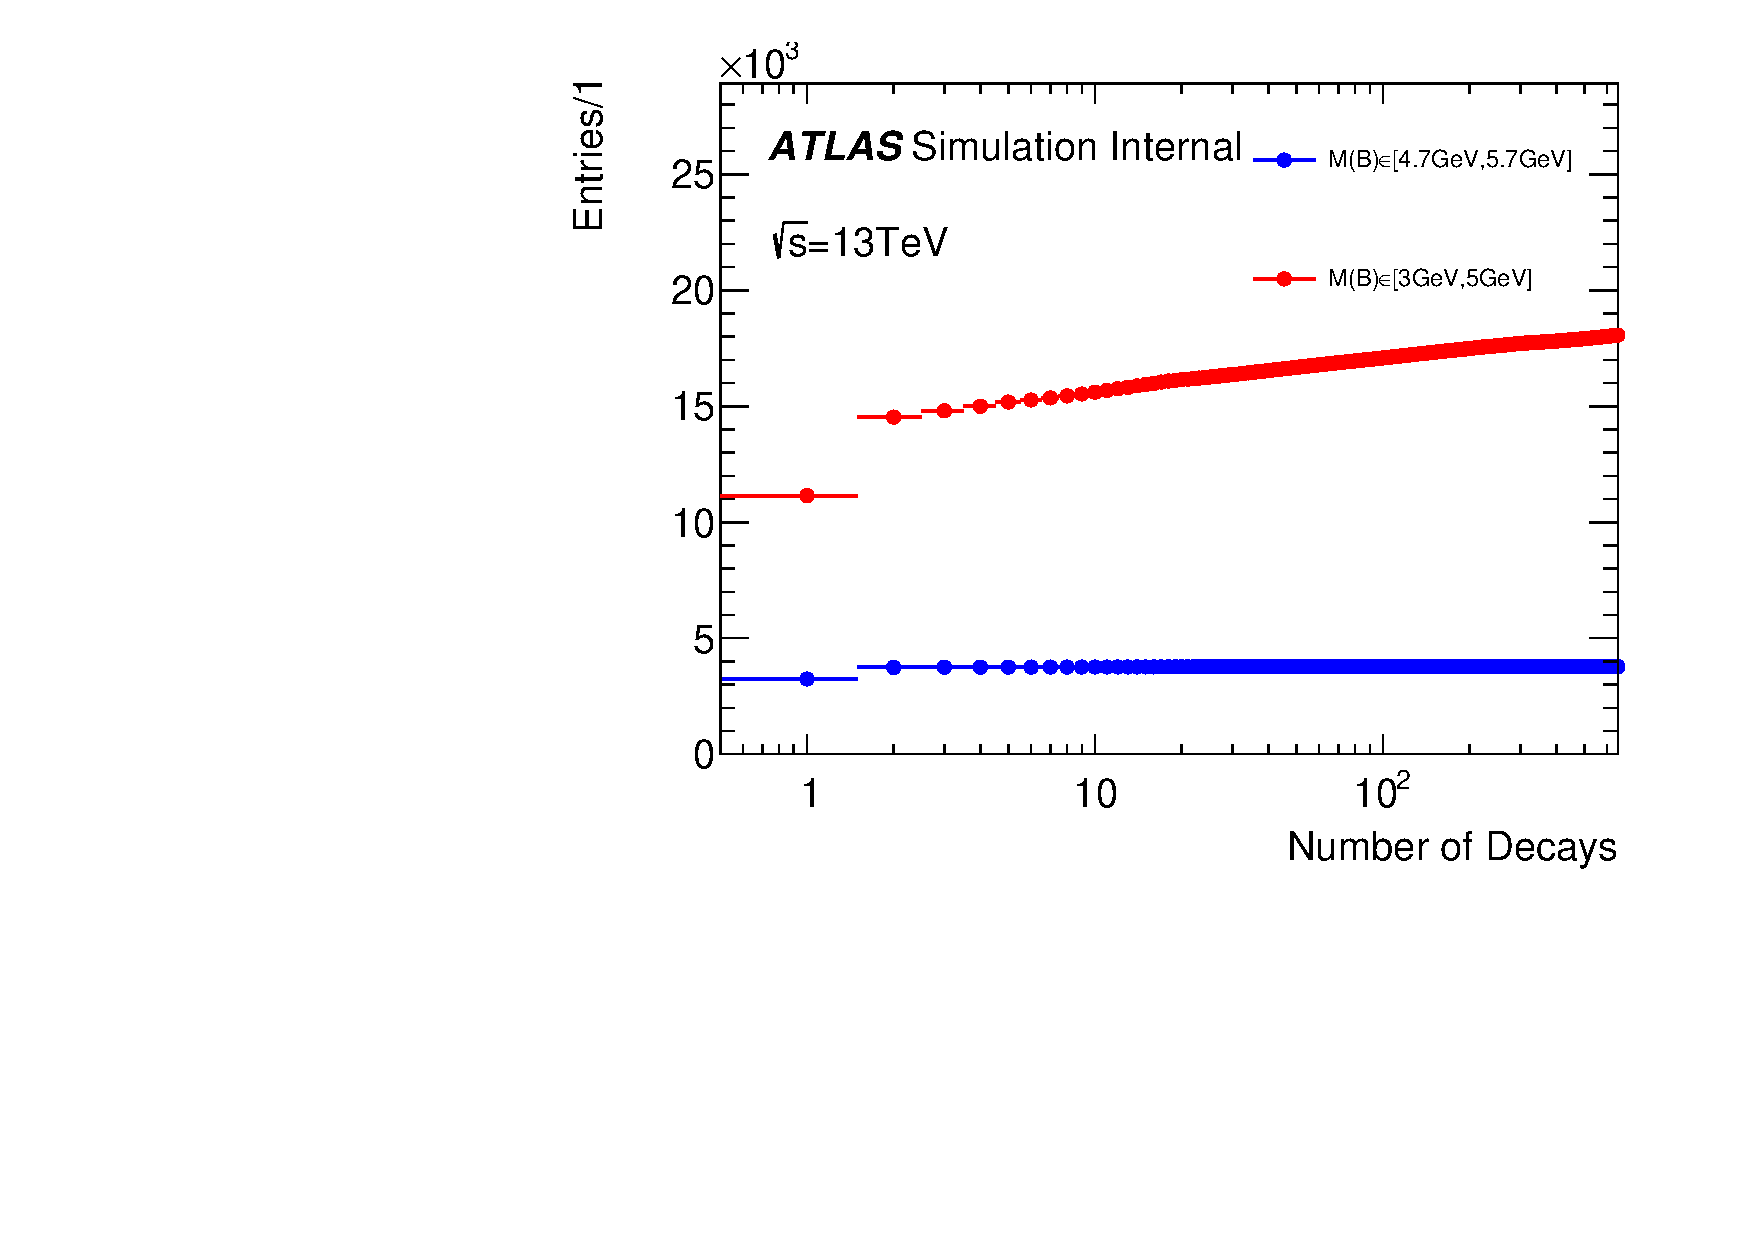
\includegraphics[width=0.45\textwidth]{bsmumu_decay_dist/cumul_entries}
    }
    \subfloat[\scriptsize $B^{+}\rightarrow J/\psi K^{+}$]
    {
	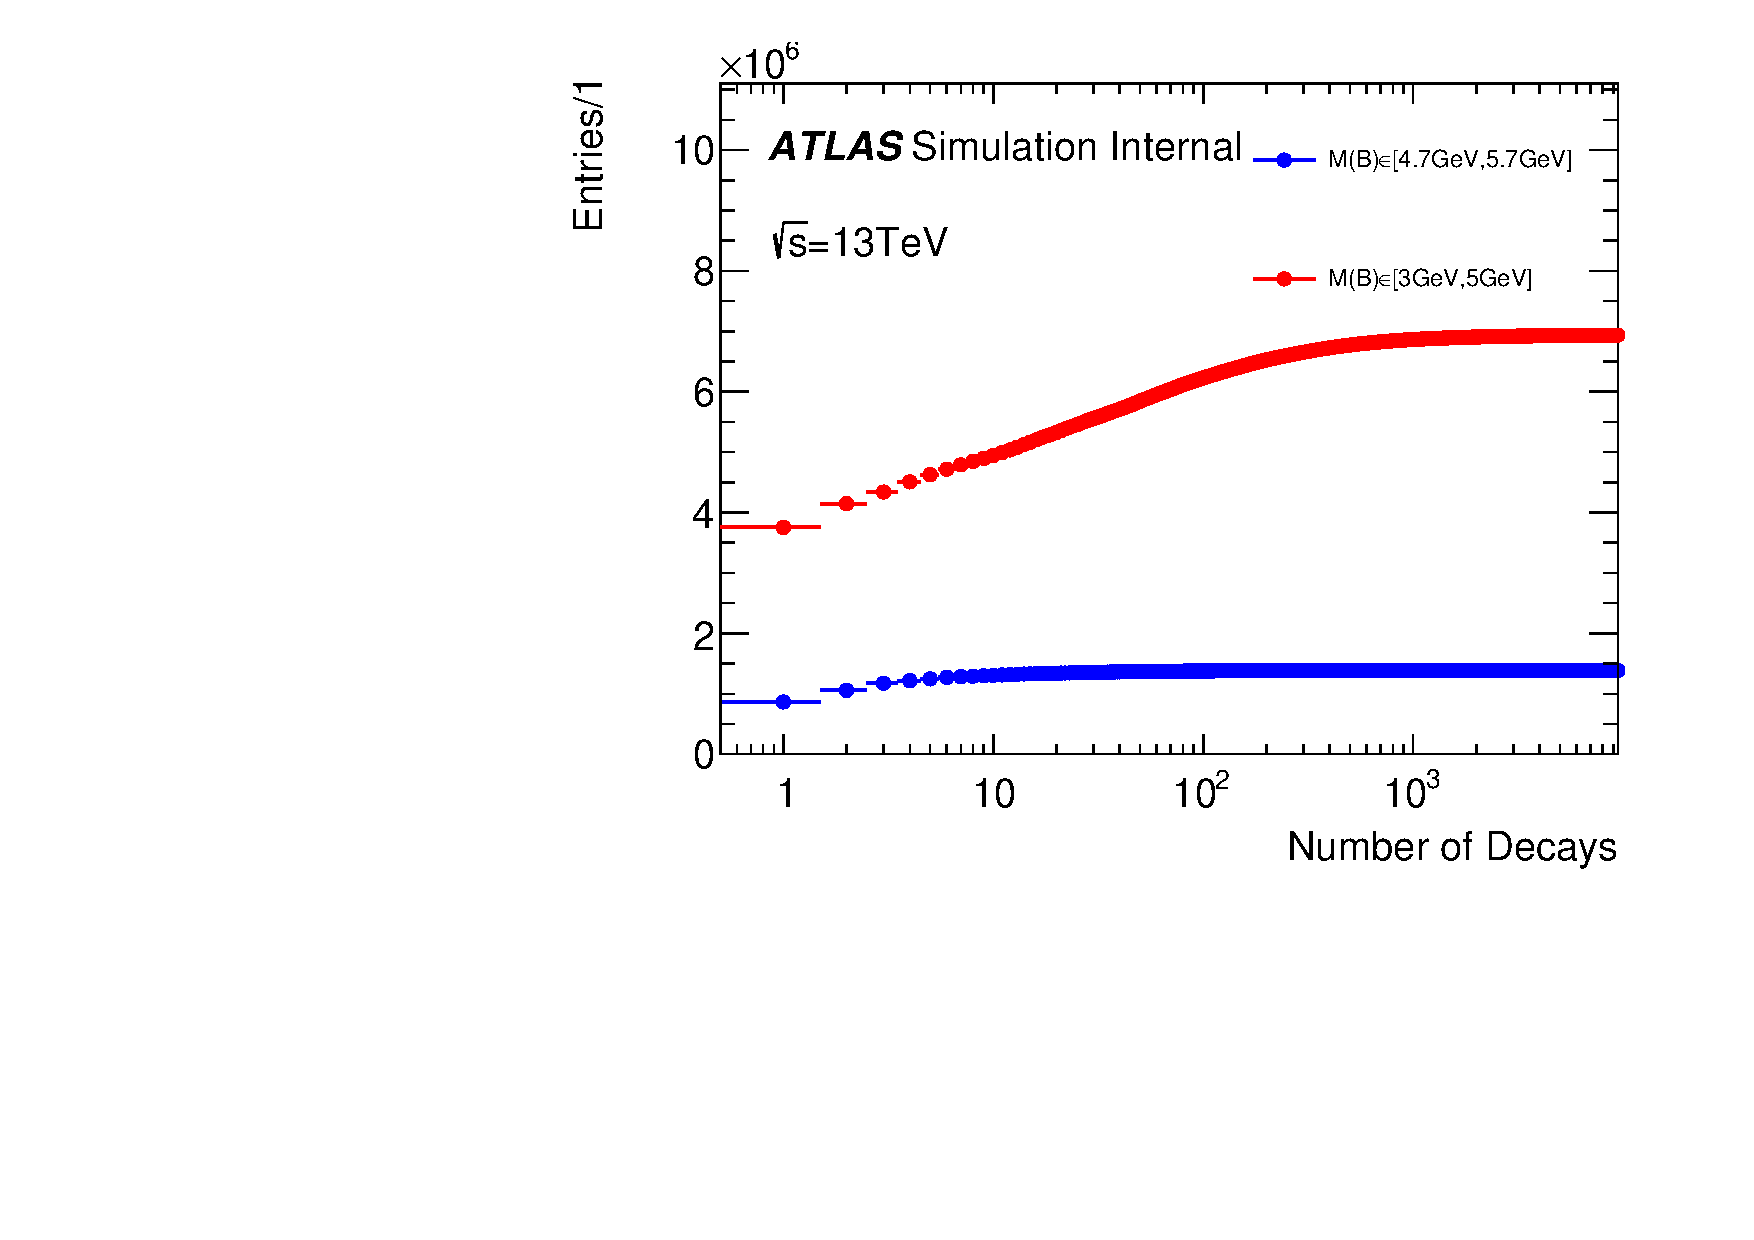
\includegraphics[width=0.45\textwidth]{bplus_decay_dist/cumul_entries}
    }

    \subfloat[\scriptsize $B_{s}\rightarrow J/\psi \phi$]
    {
	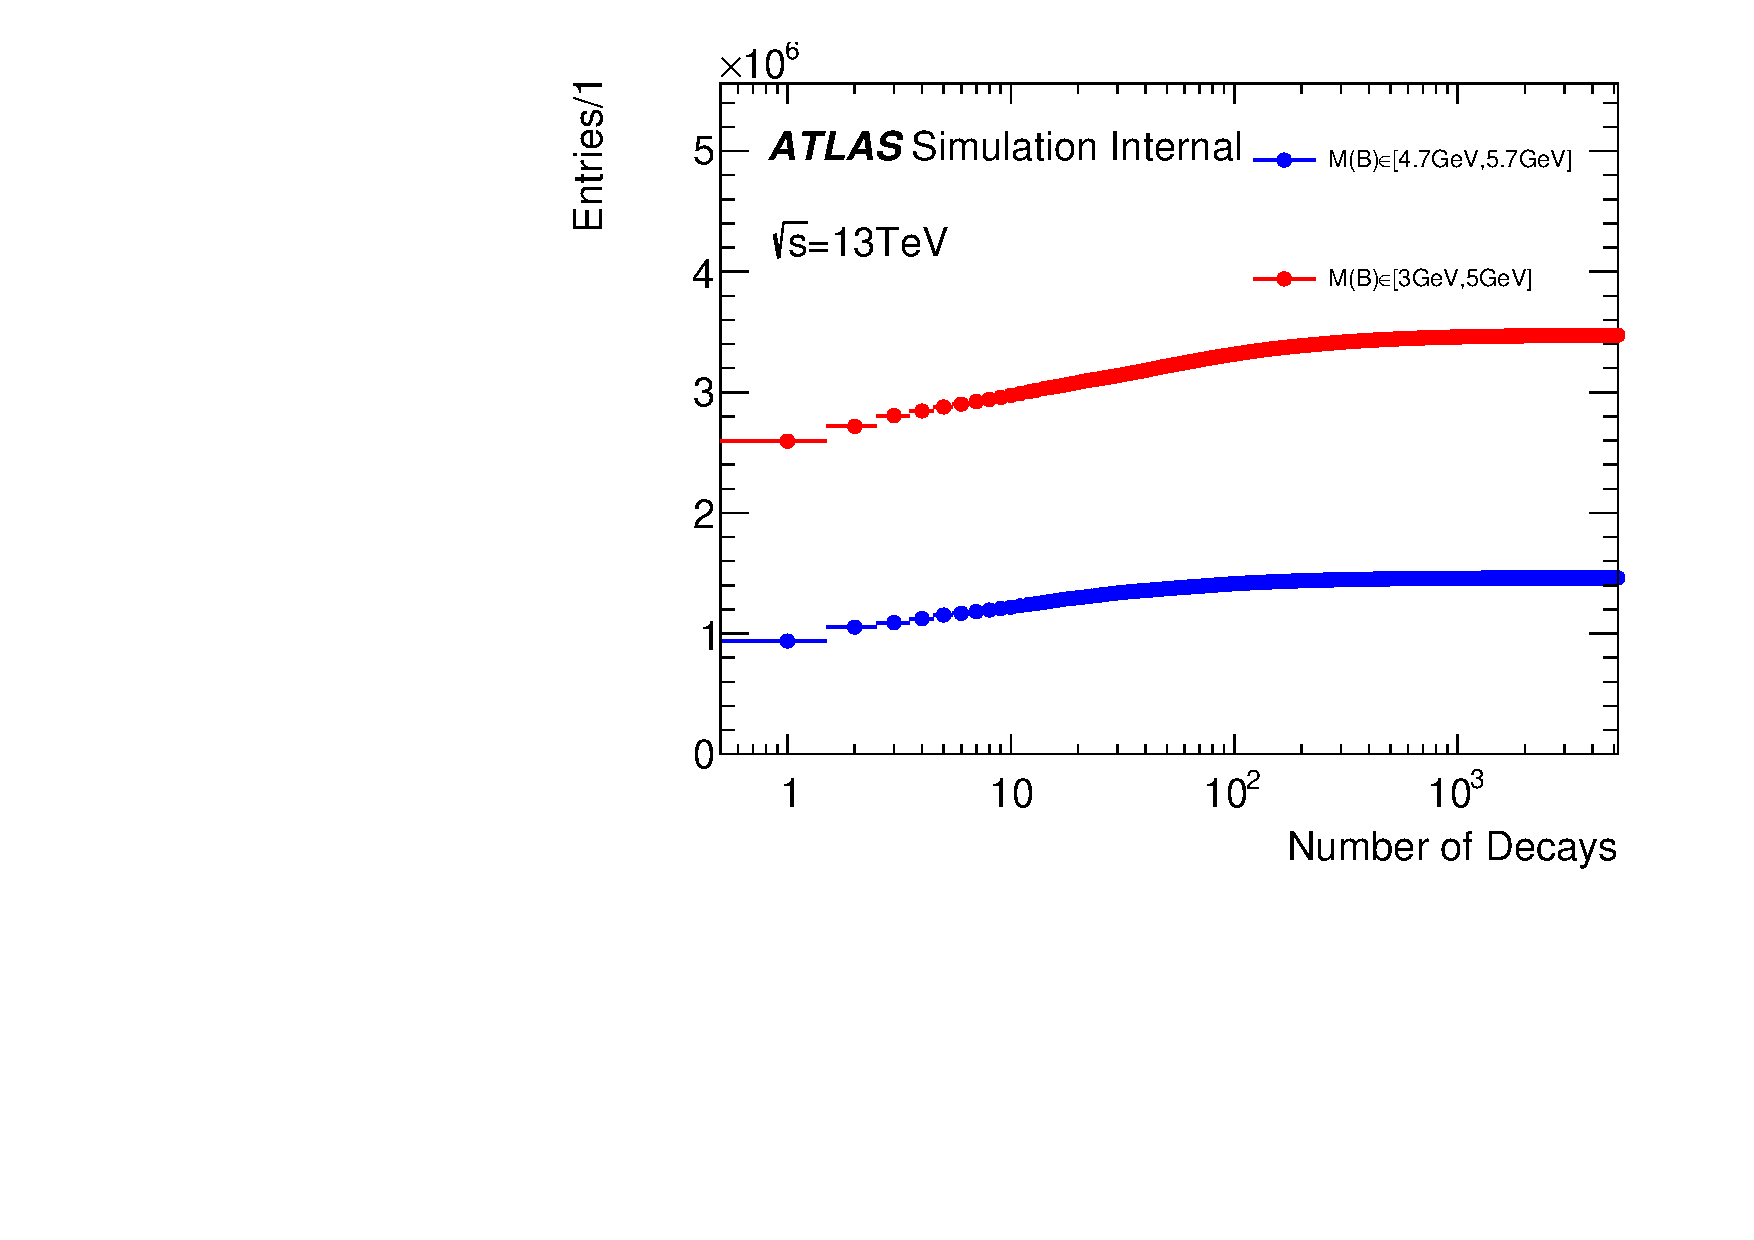
\includegraphics[width=0.45\textwidth]{bsjpsiphi_decay_dist/cumul_entries}
    }
    \caption{\scriptsize Both figures above show the cumulative number of events per decay. The first bin
	has all the events for decay number 1. The next bin, those plus decay 2, etc. The decays are ordered
    in decreasing order of events.}
    \label{fig:decay_multiplicity}
\end{figure}

Table \ref{tab:bpjpsik_decays} shows the main sources of background for $\bpjpsik$.
Table \ref{tab:bsjpsiphi_decays} shows the same for $\bsjpsiphi$. In these tables
\textit{unmatched} refers to decays in which the matching could not be made. This
happens because one of the hadron tracks, identified as the $K^+$, corresponds to
a particle that was removed from the samples during the derivation. In order to 
slim the truth particles container, particles that do not come from a $B$ decay
are removed. In practice this means that unmatched candidates can be classified
as combinatorial background. This can be seen in figure \ref{fig:unmatched_combinatorial}.

\begin{table}
    \centering
    \begin{tabular}{| l | r |}
	\hline
	Process                                           &     Candidates\\
	\hline
	unmatched                                         &         864837\\
	B+[K+:Jpsi[mu+:mu-]]                              &         192462\\
	B0[K*0[pi-:K+]Jpsi[mu+:mu-]]                      &         117439\\
	combinatorial                                              &          41869\\
	B+[K*+[pi0[gamma:gamma]K+]Jpsi[mu+:mu-]]          &          30063\\
	B+[K+:chi\_1c[gamma:Jpsi[mu+:mu-]]]                &         26241\\
	B+[K+:psi'[pi-:pi+:Jpsi[mu+:mu-]]]                &           9477\\
	B0[K*0[pi-:pi-:gamma:K+:K+]Jpsi[mu+:mu-]]         &           8545\\
	B0[pi-:K+:Jpsi[mu+:mu-]]                          &           7886\\
	B0[K*\_20[pi-:K+]Jpsi[mu+:mu-]]                    &          7435\\
	B+[pi+:Jpsi[mu+:mu-]]                             &           5956\\
	B+[K*+[pi+:K0[K\_L0]]Jpsi[mu+:mu-]]                &          5198\\
	B+[K*+[pi+:K0[K\_S0]]Jpsi[mu+:mu-]]                &          5087\\
	B+[K+:psi'[pi0[gamma:gamma]pi0[gamma:gamma]Jpsi[mu+:mu-]]]&   4811\\
	B+[rho+[pi0[gamma:gamma]pi+]Jpsi[mu+:mu-]]        &           3022\\
	\hline
    \end{tabular}
    \caption{Processes most commonly misidentified as $\bpjpsik$.}
    \label{tab:bpjpsik_decays}
\end{table}

\begin{table}
    \centering
    \begin{tabular}{| l | r |}
	\hline
	Process                                           &     Candidates\\
	\hline
	unmatched                                         &         759877\\
	B0[K*0[pi-:K+]Jpsi[mu+:mu-]]                      &         147001\\
	combinatorial                                              &          49979\\
	B0[Jpsi[mu+:mu-]K\_10[rho-[pi-:pi0[gamma:gamma]]K+]]&          43372\\
	B+[Jpsi[mu+:mu-]K\_1+[rho0[pi-:pi+]K+]]            &          33521\\
	B0[pi-:K+:Jpsi[mu+:mu-]]                          &          17924\\
	B0[K*0[pi-:K+]psi'[pi-:pi+:Jpsi[mu+:mu-]]]        &          16922\\
	B+[Jpsi[mu+:mu-]K\_1+[pi+:K*0[pi-:K+]]]            &          16325\\
	B0[pi-:K+:psi'[pi-:pi+:Jpsi[mu+:mu-]]]            &          14931\\
	B0[K*\_20[pi-:K+]Jpsi[mu+:mu-]]                    &          14856\\
	B+[K+:psi'[pi-:pi+:Jpsi[mu+:mu-]]]                &          13086\\
	B+[Jpsi[mu+:mu-]K\_1+[omega[pi-:pi0[gamma:gamma]pi+]K+]]&          12826\\
	B0[pi-:K+:chi\_1c[gamma:Jpsi[mu+:mu-]]]            &          12027\\
	B\_s0[phi[K-:K+]Jpsi[mu+:mu-]]                     &          11752\\
	B0[K*0[pi-:pi-:gamma:K+:K+]Jpsi[mu+:mu-]]         &          11022\\
	\hline
    \end{tabular}
    \caption{Processes most commonly misidentified as $\bsjpsiphi$.}
\end{table}

\begin{figure}[ht]
    \centering
    \subfloat[Combinatorial]
    {
	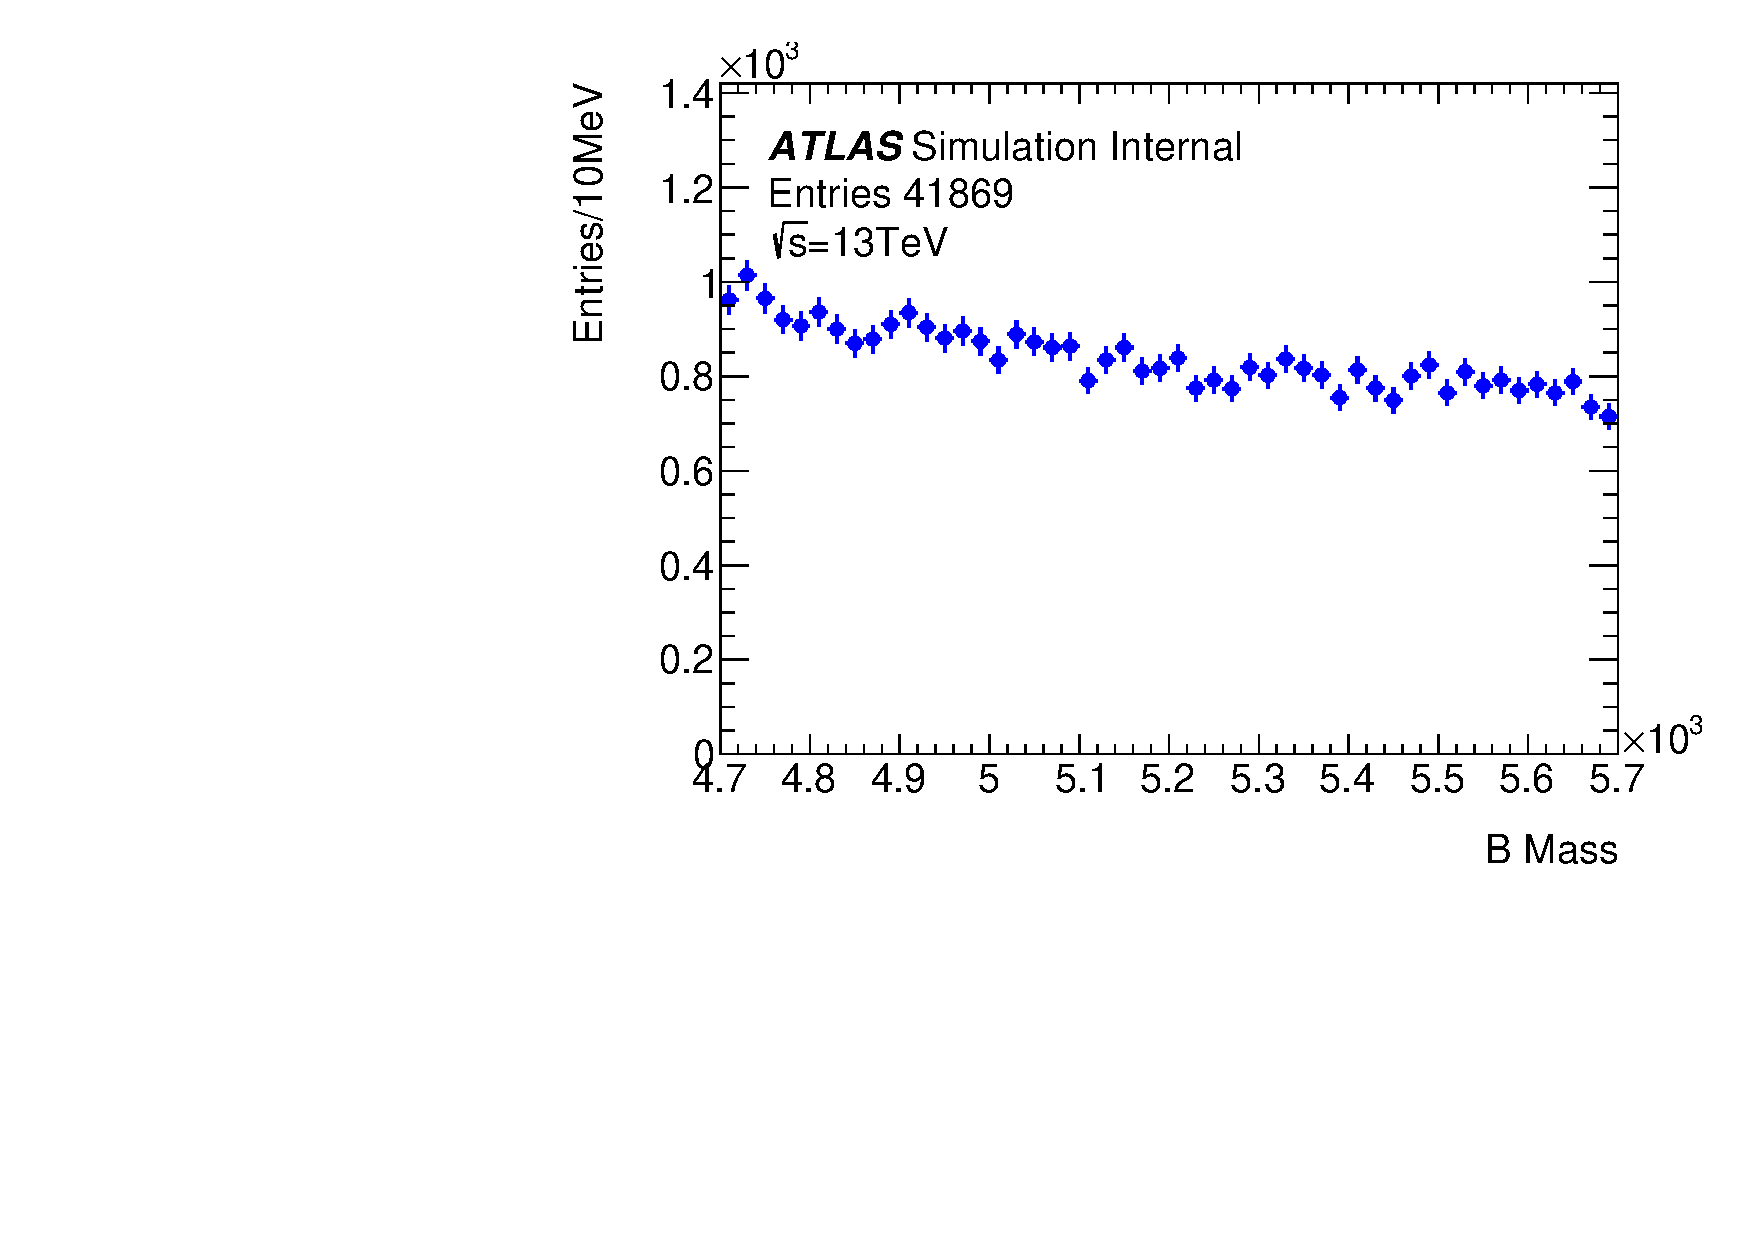
\includegraphics[width=0.45\textwidth]{bplus_components/narrow__41869__comb.pdf}
    }
    \subfloat[Unmatched]
    {
	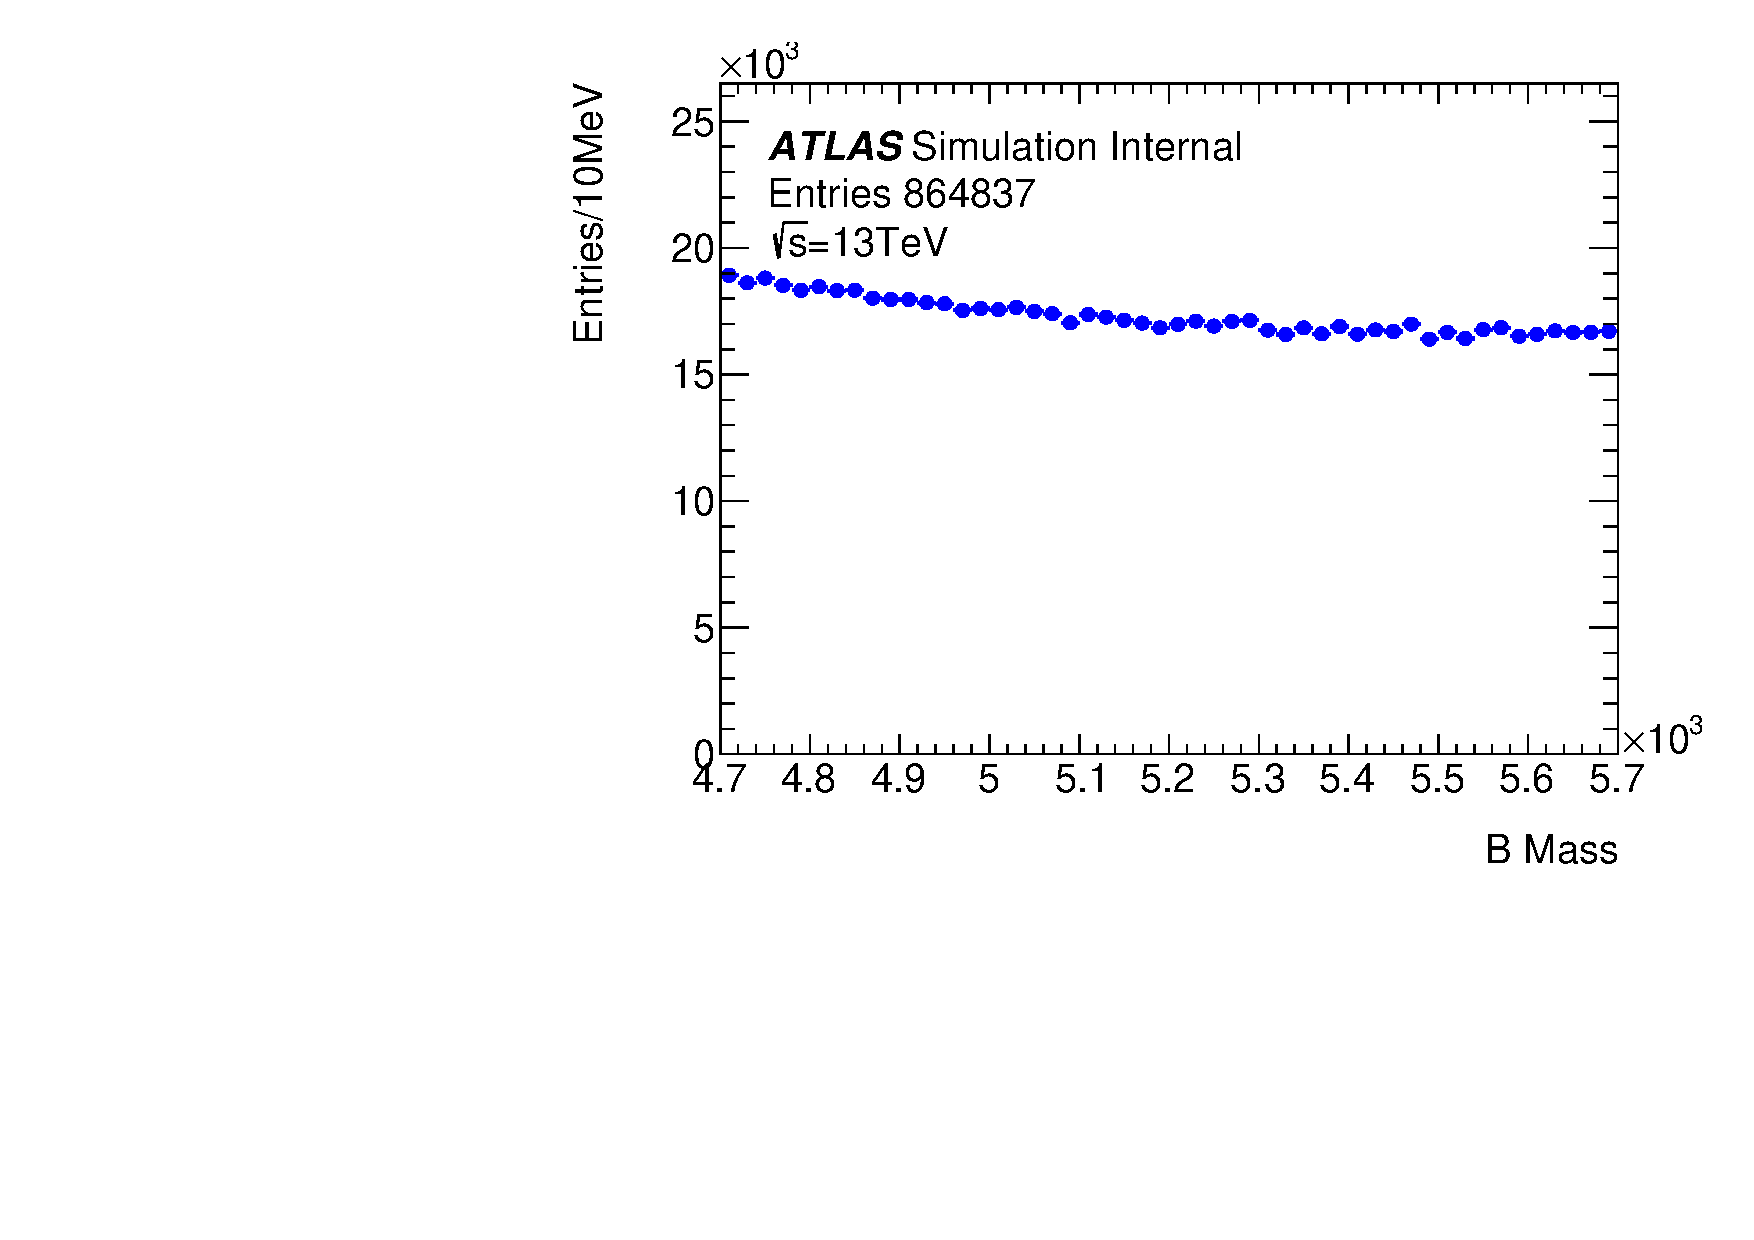
\includegraphics[width=0.45\textwidth]{bplus_components/narrow__864837__unmatched.pdf}
    }
    \caption{\scriptsize The figures show the mass distributions of $B$ candidates classified as
    \textit{combinatorial} and \textit{unmached}. Both distributions are identical in shape.}
    \label{fig:unmatched_combinatorial}
\end{figure}

\clearpage

% BDT training
\section{ContinuumBDT}
\label{sec:ContinuumBDT}
% \newcommand{\Bsmumu}{\ensuremath{B_s^0 \to \mu^+\mu^-}\xspace}

In order to discriminate against the continuum background we
employ a Multi-Variate Analysis (MVA) strategy, based on a boosted decision tree (BDT)
algorithm, as implemented in the TMVA~\cite{Hoecker:TMVA} package of ROOT. We use
$15$ physical input variables to obtain the signal-to-background discriminator. These  $15$ input 
variables are summarised in Table~\ref{tab:15vars} along with a short description of each variable.
The BDT ranking of input variable importance is given in Table ~\ref{tab:VarImportance} and compared to 
the separation power of the signal and background.
  
The following summarises the input variables which were considered for use in the
BDT. After discussing the individual variables, details of training and validation
of the classifier are given.
  
The variables can be subdivided into two groups, one related to isolation properties
of the $B$ candidates or the final state particles, and another describing topological
and kinematic properties of the \Bsmumu decay.
  
To check the isolation of the signal decay we look at non-signal tracks in the vicinity
of reconstructed B vertices, excluding the tracks associated to the pile-up vertices.
The procedure of computation of the variable, outlined in section~\ref{ssec:CandidateBuildingByDerivation} 
requires information from all tracks in an event and therefore performed on the derivation level.

\yel[t.b.c.]{Since individual muons in the signal decay are fairly well separated, isolation variables
of individual muon candidates have also been considered. However, they were rejected
in the final training, since the $B$ isolation variable $I_{0.7}$, highly correlated
to the single-muon isolation variables, contains nearly all the separation power of this
type of variables by itself.}
  
% In the computation of the $I_{0.7}$ variable we employ our own track-to-PV association
% algorithm, similar to the $B$ vertex association described above. In this way, the
% $I_{0.7}$ variable results to be robust against pile-up events. The corresponding
% requirement on the track-to-PV association was re-optimised due to the larger pile-up
% in 2012 data. We have tightened the cut on the $\ln\chi^2$ value to be less than $5$
% (instead of $6$ used in the analysis of 2011 data), which gave the best performance
% in signal/background separation.
  
The other $12$ variables in Table~\ref{tab:15vars} are related to B-decay topology and
kinematics. They were chosen from the larger pool of variables as the ones ensuring
the best BDT performance.
The variables that have been considered but dismissed are listed below for future
reference: they do not contribute significantly to the signal/background separation,
either by nature or due to the presence of other strongly correlated but more powerful
variables.
   
\begin{itemize}
\setlength{\itemsep}{0pt}%
\setlength{\parskip}{0pt}%
\item $L_{xy}$ significance
\item flight length significance in 2D and 3D
\item $d_0^{Max}$, $d_0^{Min}$
\item the significance of the closest track DOCA
\item $\chi^2$ between PV and B vertex in $z$ 
\item $p_{T}^{B}$ significance
%$B$ transverse momentum significance
% 1 BvtxPointingAngle3D a_3D pointing angle in 3D 
\item   pointing angle $|\alpha_{3D}|$
%       Absolute value of the angle between $\Delta\overrightarrow{x}$ and $\overrightarrow{p}^{B}$ & new \\ \\
% 15 BvtxChi2byNDF B_fitChi2NDF chi2/NDF of B vertex 
\item B vertex fit $\chi^2_B$/NDF
%$\chi^2$/NDF of the $B$ vertex & new \\
\item coplanarity of \Bsmumu' decays
\item coplanarity of \Bsmumu' decays with $Z$-axis
\item minimum signed $d_0$ significance of the signal candidate
\end{itemize}
Lastly in order to arrive at the BDT to
use for this analysis, a number of configurations have been studied, and
the best (with respect to background rejection and algorithm behavior)
has been selected for use in the final result.
 
\begin{table}[!htb]
\begin{center}
\begin{tabular}{p{2cm} p{10.9cm} p{2.1cm}}
\hline \hline
Variable  &  Description \\ 
\midrule
% 1. TMath::Abs(BvtxPointingAngle2D) TMath::Abs(a_2D) angle btw. dX and pB in xy plane used in 2011 analysis
$|\alpha_{2D}|$ & Absolute value of the angle in the transverse plane
between $\Delta\overrightarrow{x}$ and $\overrightarrow{p}^{B}$ \\ \\   
% 2. BvtxIsolation B_iso_7_Chi2_5_MedPt05 isolation of B candidate used in 2011 analysis(*)
Isolation $I_{0.7}$ & Ratio of $|\overrightarrow{p}^{B}_{T}|$ to the sum of $|\overrightarrow{p}^{B}_{T}|$ and
the transverse momenta of all tracks with $p_T > 0.5$ GeV within a
cone $\Delta{R} < 0.7$ from the $B$ direction, excluding $B$ decay products  \\ \\  
% 3. BvtxDR DR sqrt(df^2+deta^2) btw. dX and pB used in 2011 analysis
$\Delta{R}$ & Angle $\sqrt{\left(\Delta\phi\right)^{2} + \left(\Delta\eta\right)^{2}} $
between $\Delta\overrightarrow{x}$ and $\overrightarrow{p}^{B}$ \\ \\  
% 4.  BvtxPt B_pT pT of B candidate used in 2011 analysis
$p_{T}^{B}$ & $B$ transverse momentum  \\ \\  
% 5.  minChi2MuonsIP2AnyPV B_minChi2MuonsIPtoAnyPV
$\chi^2_{\mu,xPV}$ & Minimum $\chi^2$ between the muon candidates and any PV  \\  
% 6. lnChi2PVtxBVtx2D chi2_PVSV_log2D chi2 btw. PV and SV in xy used in 2011 analysis
%        $\chi^{2}_{z}, \chi^{2}_{xy}$ & Significance of the separation between production
%        (PV) and decay (SV) vertices, $\Delta\overrightarrow{x}^{T}\cdot
%        \left(\sigma^{2}_{\Delta\overrightarrow{x}}\right)^{-1}\cdot\Delta\overrightarrow{x}$,
%        in $z$ and $(x,y)$, respectively & used in $2011$\\ \\
$\log[\chi^{2}_{\mathrm{PV,SV}}]_{xy}$ & separation between production
(PV) and decay (SV) vertices, $\Delta\overrightarrow{x}^{T}\cdot
\left(\sigma^{2}_{\Delta\overrightarrow{x}}\right)^{-1}\cdot\Delta\overrightarrow{x}$,
in the transverse plane $(x,y)$ \\ \\  
% 7. Bvtx3DIP Bvtx3DIP 3D impact parameter (POCA) of B candidate
IP$_B^{3D}$ & 3-dimensional impact parameter (POCA) of the $B$ candidate \\  
% 8. TMath::Abs(d0MaxSign) d0Max_sig IP significance of the muon track with max IP
$|d_{0}|^{max}$ sig. & Significance of the maximum absolute value of impact
parameters of the two muon candidates in the transverse plane of the $B$
decay products relative to the primary vertex \\  
% 9. TMath::Abs(MuonsRefTrksDPhi) B_IDtrks_deltaPhi &Delta(&phi,&mu1 - &phi,&mu2)
$\Delta\phi(\mu\mu)$ & Difference in $\phi$ between the two muon candidates  \\  
% 10. ClosTrackDOCA closeTrkDOCA DOCA of the track closest to B vertex
DOCA$_{xtrk}$ & DOCA of the track closest (``xtrk'') to the $B$ vertex.
The tracks associated to pile-up vertices are excluded \\  
% 11. TMath::Abs(MuonsDCA) TMath::Abs(B_IDtrks_DCA) DCA ot two ID tracks forming B vertex
DOCA$_{\mu\mu}$ & DOCA of the two ID tracks forming the $B$ vertex  \\  
% 12. ClosTrackNTracksChi2 closeTrkNtrksChi2 chi2 btw. the closest track and B vertex
%        $\chi^2_{B,xtrk}$ & $\chi^2$ between the closest track and the $B$ vertex  & new \\
$N^{close}_{trks}$ & Number of (``close'') tracks with $\ln(\chi^2)<1$ where
$\chi^2$ is a test of association of a track to the reconstructed $B$ vertex.
The tracks associated to pile-up vertices are excluded\\  
% 13. TMath::Abs(d0MinSign) d0Min_sig IP significance of the muon track with min IP
$|d_{0}|^{min}$ sig. & Significance of the minimum absolute value of impact
parameters of the two muon candidates in the transverse plane of the $B$
decay products relative to the primary vertex\\  
% 14. BvtxLxy Lxy (dxp)xy/pt used in 2011 analysis
$L_{xy}$ & Scalar product in the transverse plane of
$(\Delta\overrightarrow{x}\cdot\overrightarrow{p}^{B})/|\overrightarrow{p}^{B}_{T}|$\\ \\  
% 15. BvtxPlngMin2D PlngMin2D minimum momentum of the two muon candidates along the B direction used in 2011 analysis
%        $P_{L}^{min}, P_{L}^{max}$ & Minimum and maximum momenta of
%        the two muon candidates along the $B$ direction & used in $2011$\\ \\
$P_{L}^{min}$ & Minimum momentum of the two muon candidates
along the $B$ direction\\ \\
\hline \hline
\end{tabular}
\caption{Description of the $15$ discriminating variables used in the
discrimination between signal and continuum background.}
\label{tab:15vars}
\end{center}
\end{table}

\begin{table}[!htb]
\begin{center}
%CMD+l lift then press j - sync to pdf on skim
%on skim CMD-Shift click - sync back to ST (sublime text)
%build latex with CMD+b
%CMD+l lift then press delete - remove aux files from folder!!
%Installed LaTexTools and LaTex-clw for autocomplete

\documentclass[12pt]{article} %[12pt]
%compile using LuaLaTex from drop down menu
% comment multiple lines using \iffalse *multiple lines of text*  \fi
\usepackage{tikz}
\usepackage{tikz-feynman}
\tikzfeynmanset{compat=1.0.0}
\usepackage{caption}
\usepackage{subcaption}
\usepackage{float}
%\usepackage{atlasphysics}
%Bibliography preamble
\usepackage[numbers,sort&compress]{natbib}
%geometry of margins
\usepackage[left=1in,right=1in,top=1in,bottom=0.5in]{geometry}
\usepackage{url}
\usepackage{amsmath}
\usepackage{bm}
\usepackage{amssymb}
\usepackage{mathtools}
\usepackage[utf8]{inputenc}
\usepackage{longtable}

\newcommand*{\TitleFont}{%
      %\usefont{\encodingdefault}{\rmdefault}{b}{n}%
      \fontsize{16}{20}%
      \selectfont}
%\date{December 15, 2016}
\usepackage{booktabs}
\usepackage{longtable}
\usepackage{array}
\usepackage{lscape}
\begin{document}
\begin{landscape}
\begin{longtable}{llrlr}
\toprule
Imp. Rank &                                       Variable &  Importance & Sep. Rank &  Separation \\
\midrule
\endhead
\midrule
\multicolumn{3}{r}{{Continued on next page}} \\
\midrule
\endfoot

\bottomrule
\endlastfoot
        1 &                                $|\alpha_{2D}|$ &     0.11290 &         2 &     0.57270 \\
        2 &                                     $\Delta R$ &     0.10720 &         1 &     0.59070 \\
        3 &         B Iso BEJ (PPP) Custom TVA Trk Perigee &     0.09343 &         6 &     0.39280 \\
        4 &                      $log(\chi^{2}_{\mu,xPV})$ &     0.08988 &         4 &     0.43970 \\
        5 &                            $ln(\chi^{2}_{xy})$ &     0.07679 &         9 &     0.30400 \\
        6 &                                      $p^B_{T}$ &     0.07132 &        13 &     0.02416 \\
        7 &                       $|\Delta \phi_{\mu\mu}|$ &     0.06958 &        15 &     0.01313 \\
        8 &  nCloseTracks BEL (PPP) Custom TVA Trk Perigee &     0.06658 &         3 &     0.45130 \\
        9 &                                $|IP_{B}^{3D}|$ &     0.05015 &        11 &     0.14500 \\
       10 &                                $DOCA_{\mu\mu}$ &     0.04812 &        12 &     0.07437 \\
       11 &          DOCA BEL (PPP) Custom TVA Trk Perigee &     0.04766 &         5 &     0.40100 \\
       12 &                                       $L_{xy}$ &     0.04485 &         8 &     0.37820 \\
       13 &                                  $P^{min}_{L}$ &     0.04410 &        14 &     0.02359 \\
       14 &                               $d^0_{max, sig}$ &     0.04252 &        10 &     0.17100 \\
       15 &                               $d^0_{min, sig}$ &     0.03502 &         7 &     0.39140 \\
\end{longtable}

\end{landscape}
\end{document}
\caption{The BDT ranking of input variable importance and compared with the signal and background 
separation power of each variable as calculated by TMVA before training.}
\label{tab:VarImportance}
\end{center}
\end{table}
 
Appendix~\ref{app:contBDT} summarises the correlation matrices calculated
for signal and background events for the $15$ discriminating variables used
in this analysis.
The BDT training is done using the \bbmumuX background MC (described in
%used to be sec:4corners
Sec.~\ref{sec:BackgroundModeling}) and signal MC events. All selection cuts are applied to both the combinatorial events and the signal MC events. 
 
The training is done using the TMVA tool, splitting the two input samples into
equal halves. The first half is used for training the BDT and the second for
validation.
The $1/4$th of the signal MC was kept off the training and validation samples and
it has been used for evaluation, together with the data candidates from the right
mass sideband.\footnote{To clarify, the signal MC sample events are used:
$37.5\%$ for training, $37.5\%$ for validation, and $25\%$ for evaluation.}
The left plot in Figure~\ref{fig:contBDT} shows the test for over-training,
where the BDT outputs for training and validation samples are shown, confirming that
the BDT is not over-trained as the training and validation samples are in good
agreement with each other. \yel[t.b.d.]{The right plot contains the training result via
the Receiver Operating Characteristic (ROC) curve and the comparison with the BDT
used in 2012 analysis: the new training results to be significantly more efficient.}
 
\begin{table}[htbp]
\begin{center}
\begin{tabular}{|c|c|}
\hline
Parameter & Value \\
\hline
\hline
\textit{NTrees} & 500 \\
\hline
\textit{MinNodeSize} & 1.0[\%]\\
\hline
\textit{MaxDepth} & 3 \\
\hline
\textit{BoostType} & AdaBoost \\
\hline
\textit{AdaBoostBeta} & 0.5 \\
\hline
\textit{UseBaggedBoost} & True\\
\hline
\textit{BaggedSampleFraction} & 0.6\\
\hline
\textit{SeparationType} & GiniIndex \\
\hline
\textit{nCuts} & 100\\
\hline
\textit{NormMode} & EqualNumEvents\\
\hline
\hline
\end{tabular}
\end{center}
\caption{\label{tab:cBDTPars} Configuration parameters of the \textit{continuum}-BDT.}
\end{table}
 
The final choice of the configuration parameters of the \textit{continuum}-BDT,
as used by TMVA, is shown in Table \ref{tab:cBDTPars}.
The optimal values for the configuration parameters \textit{MinNodeSize} 
and \textit{AdaBoostBeta} were found with the help of a grid scan using background rejection at 36\% signal efficiency on the ROC-curve as a figure of merit of classifier performance. The \textit{MaxDepth} parameter
has also been studied in the similar way. For this parameter, it has been found
that the performance of classifier improves with increasing
of \textit{MaxDepth}, whereas the discrepancy between its performance on the training
and testing sample, accessed by the Kolmogorov-Smirnov test, becomes larger,
leading to the over-training. In order to not compromise the generality of the classifier,
the value \textit{MaxDepth=3} has been chosen.
The value of \textit{NTrees} has been chosen large enough to allow the training to converge.
The choice of other parameters does not have any significant impact on the training result.
 
We have tested the chosen BDT configuration against different training samples including
various sample re-weighting, previous selection cuts and increase of statistics.
We found no real impact on the performance of the BDT proving that the chosen
configuration is very robust.
 
\yel[t.b.c.]{In addition we tested a BDT variable built without the use of the isolation variable
as input: the study is described in Appendix}~\ref{app:BDT-noISO}. As expected, the
separation power is reduced thus the BDT configuration described in this section is
the one used in the analysis.
 
\begin{figure}[!htb]
\begin{center}
\hspace{-0.5cm}
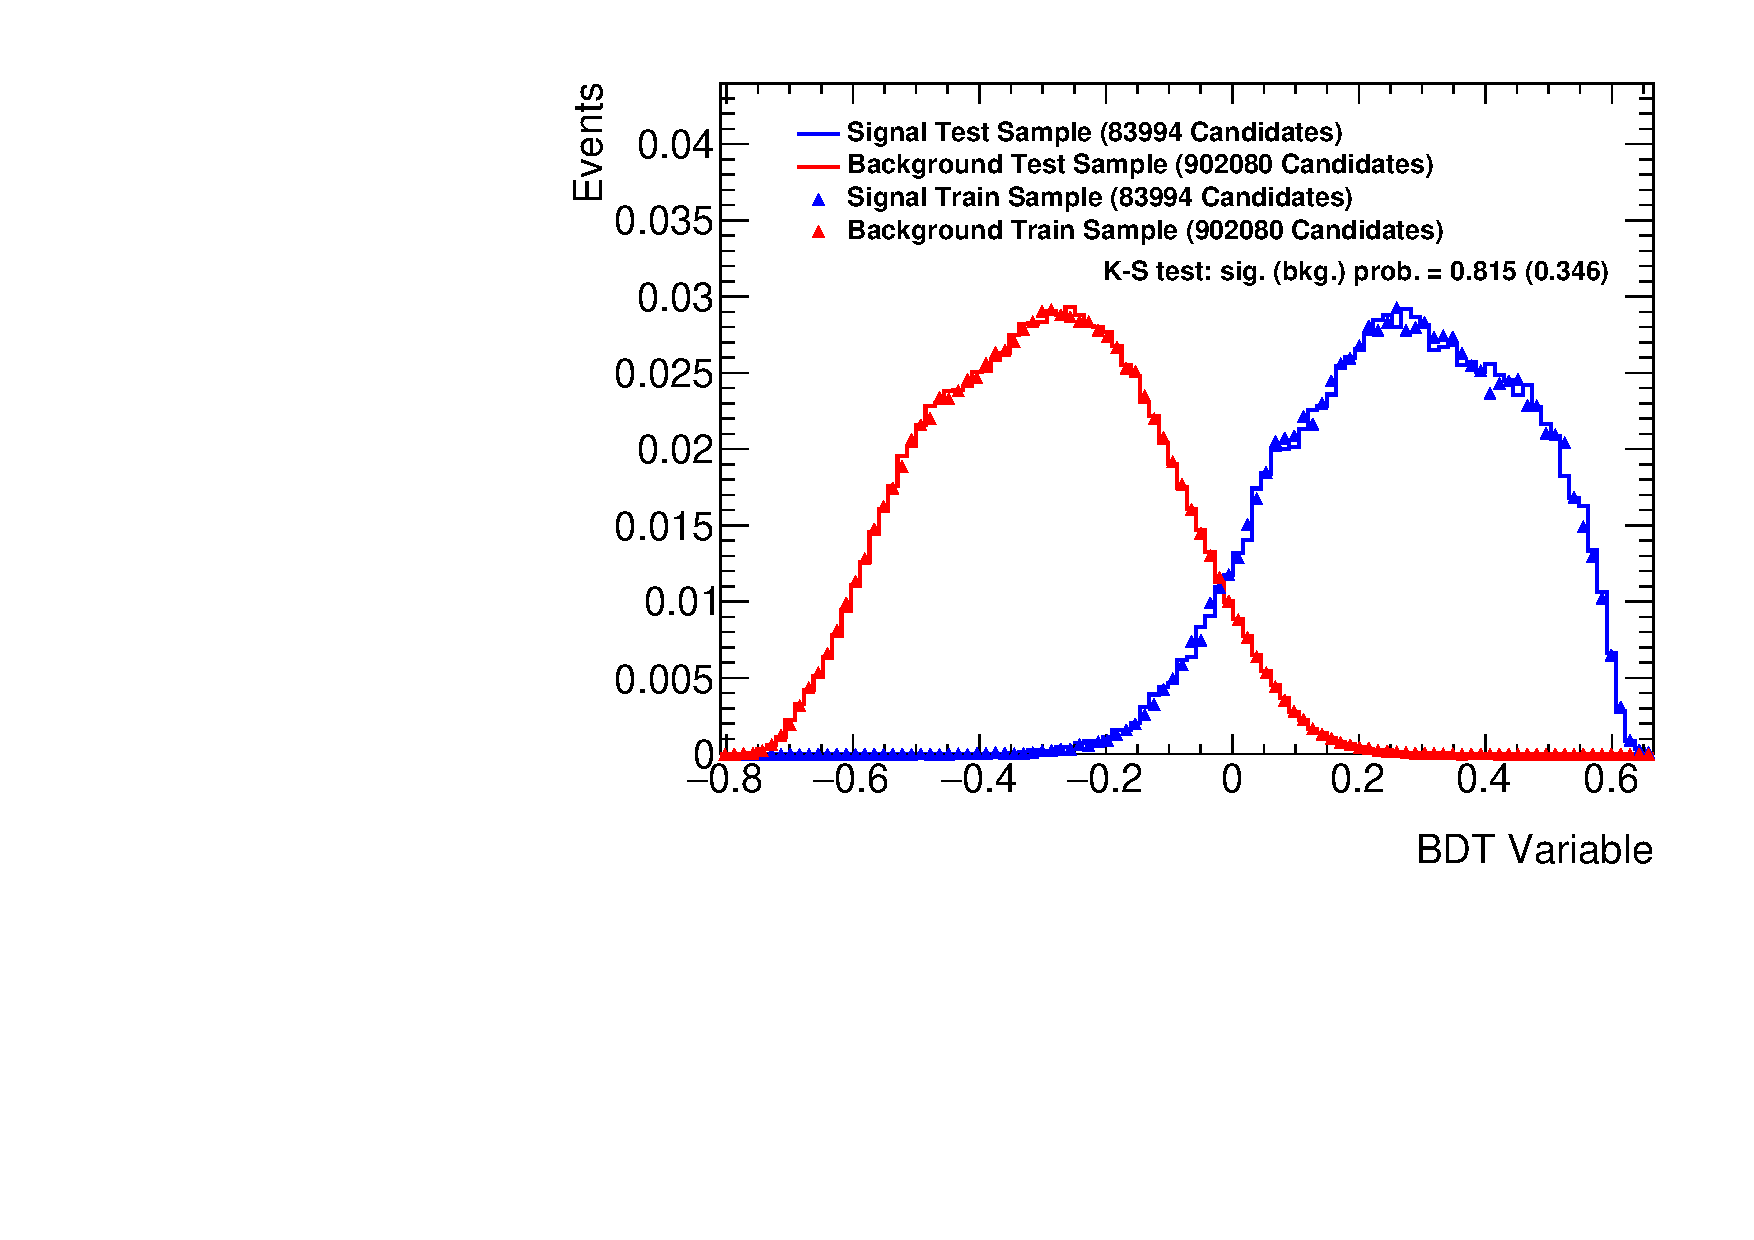
\includegraphics[width=0.52\textwidth]{figures/InternalNote_ContinuumBDT/KS.pdf}
\hspace{-0.5cm}
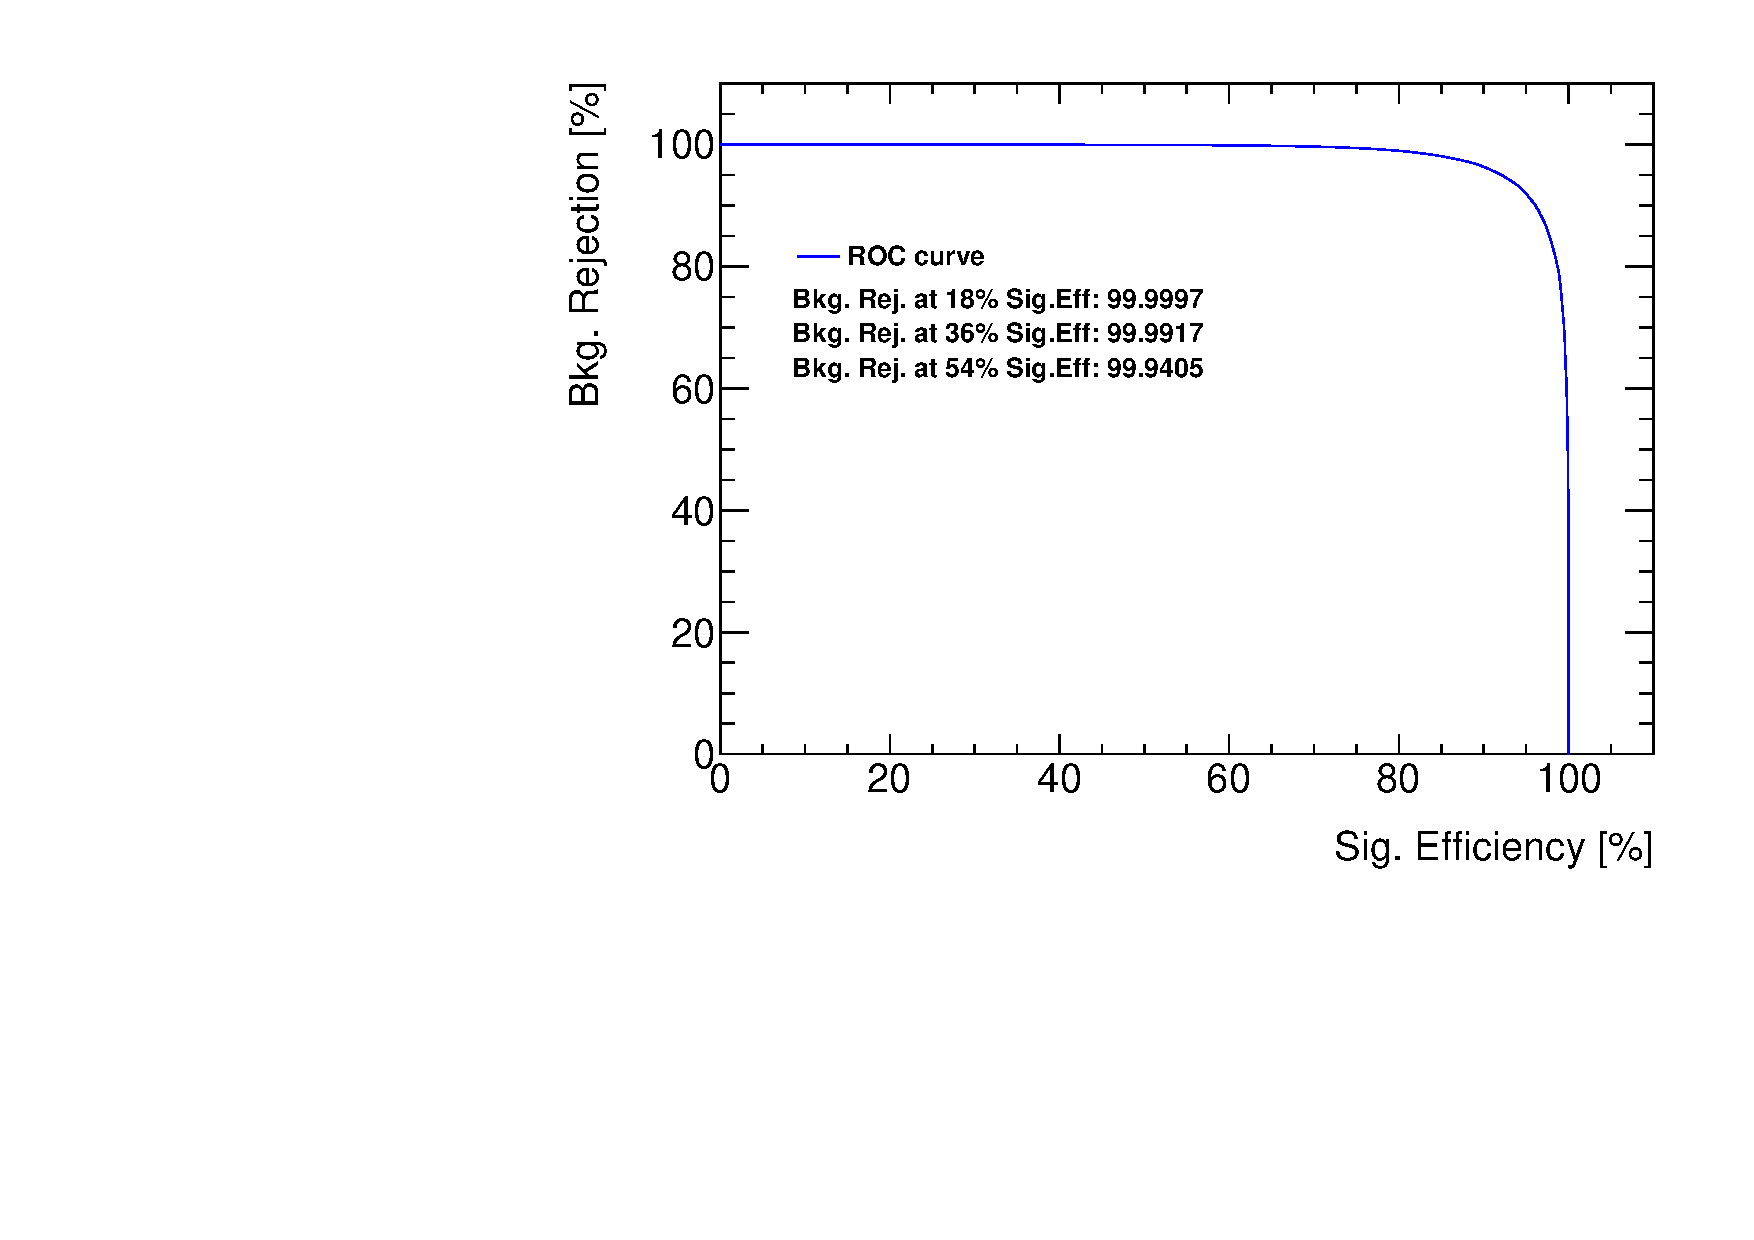
\includegraphics[width=0.52\textwidth]{figures/InternalNote_ContinuumBDT/ROC.pdf}
\caption{{\itshape Left}: cross-checks for over-training for the continuum BDT variable.
{\itshape{Right}}: \textbf{Only ROC curve at the moment!} comparison of ROC curves trained on the combinatorial background MC and the signal MC. The ROCs are evaluated on the high-mass data sideband.}
\label{fig:contBDT}
\end{center}
\end{figure}



\clearpage

% Data-MC Comparisons
\section{DataMCComparison}
\label{sec:DataMCComparison}

The shapes of distributions of the discriminating variables used to separate
out the combinatorial background are compared in data and MC samples.
This analysis is detailed in~\cite{bsmumuv2} [App. A and C].
   
\subsection{Continuum events}
\label{sec:compcont}
  
To check the shapes of the discriminating variables for the
combinatorial background we compare the signal MC sample with
the data sidebands. The signal sample is re-weighted on PV and separately on the \pt\ $^B$, $\eta$ $^B$ and B Isolation
variables simultaneously with a gradient boosted re-weighting technique~\cite{Rogozhnikov:2016bdp}.
Figure~\ref{fig:xcheckcont} shows the corrected \pt\ , $\eta$ ,  and B Isolation variables as a cross-check.
  
Figure~\ref{fig:maincompcont} shows the distributions of few
discriminating variables. The rest can be checked in
\yel[t.b.d.]{Appendix}~\ref{app:contBDT}.
  
\begin{figure}[!htb]
\begin{center}
\hspace*{-0.6cm}
% 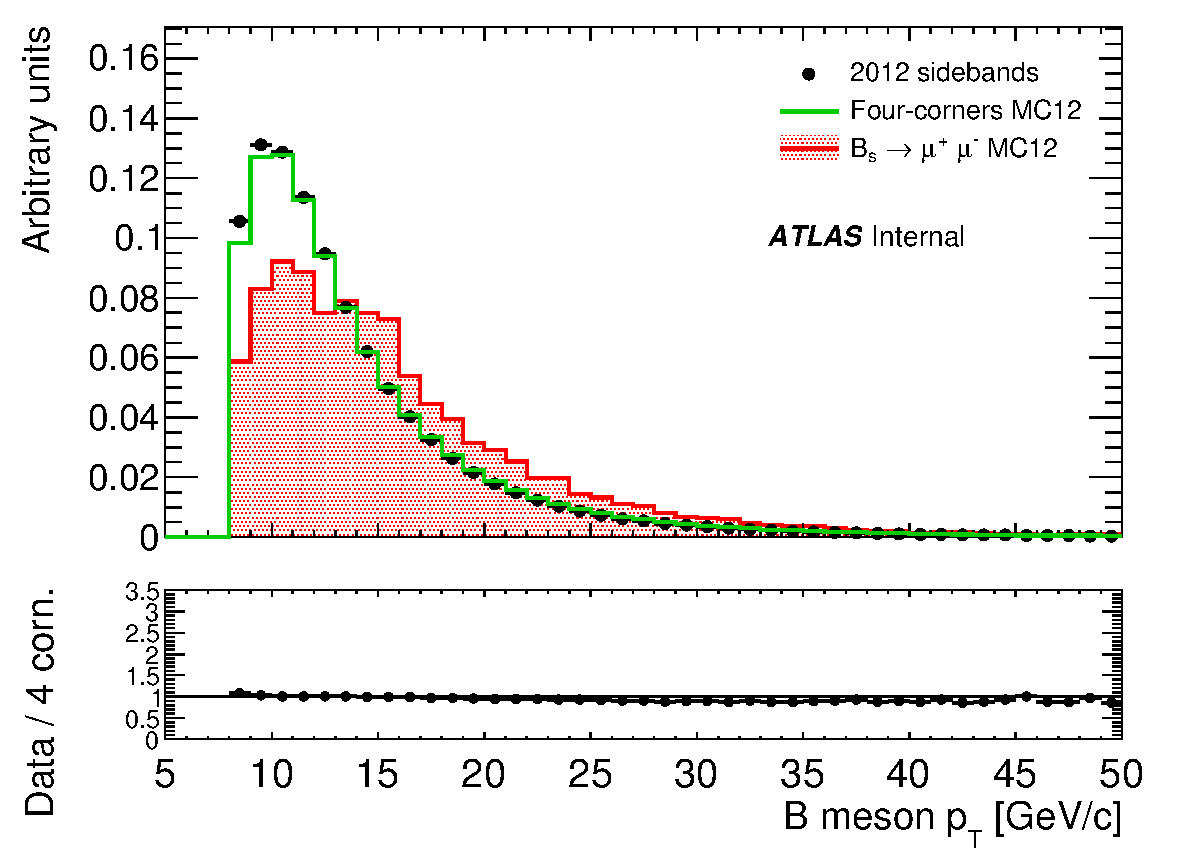
\includegraphics[width=0.52\textwidth]{figures/InternalNote_DataMCComparison/compRun1/cont/pT_data4corn_reweighted.pdf}
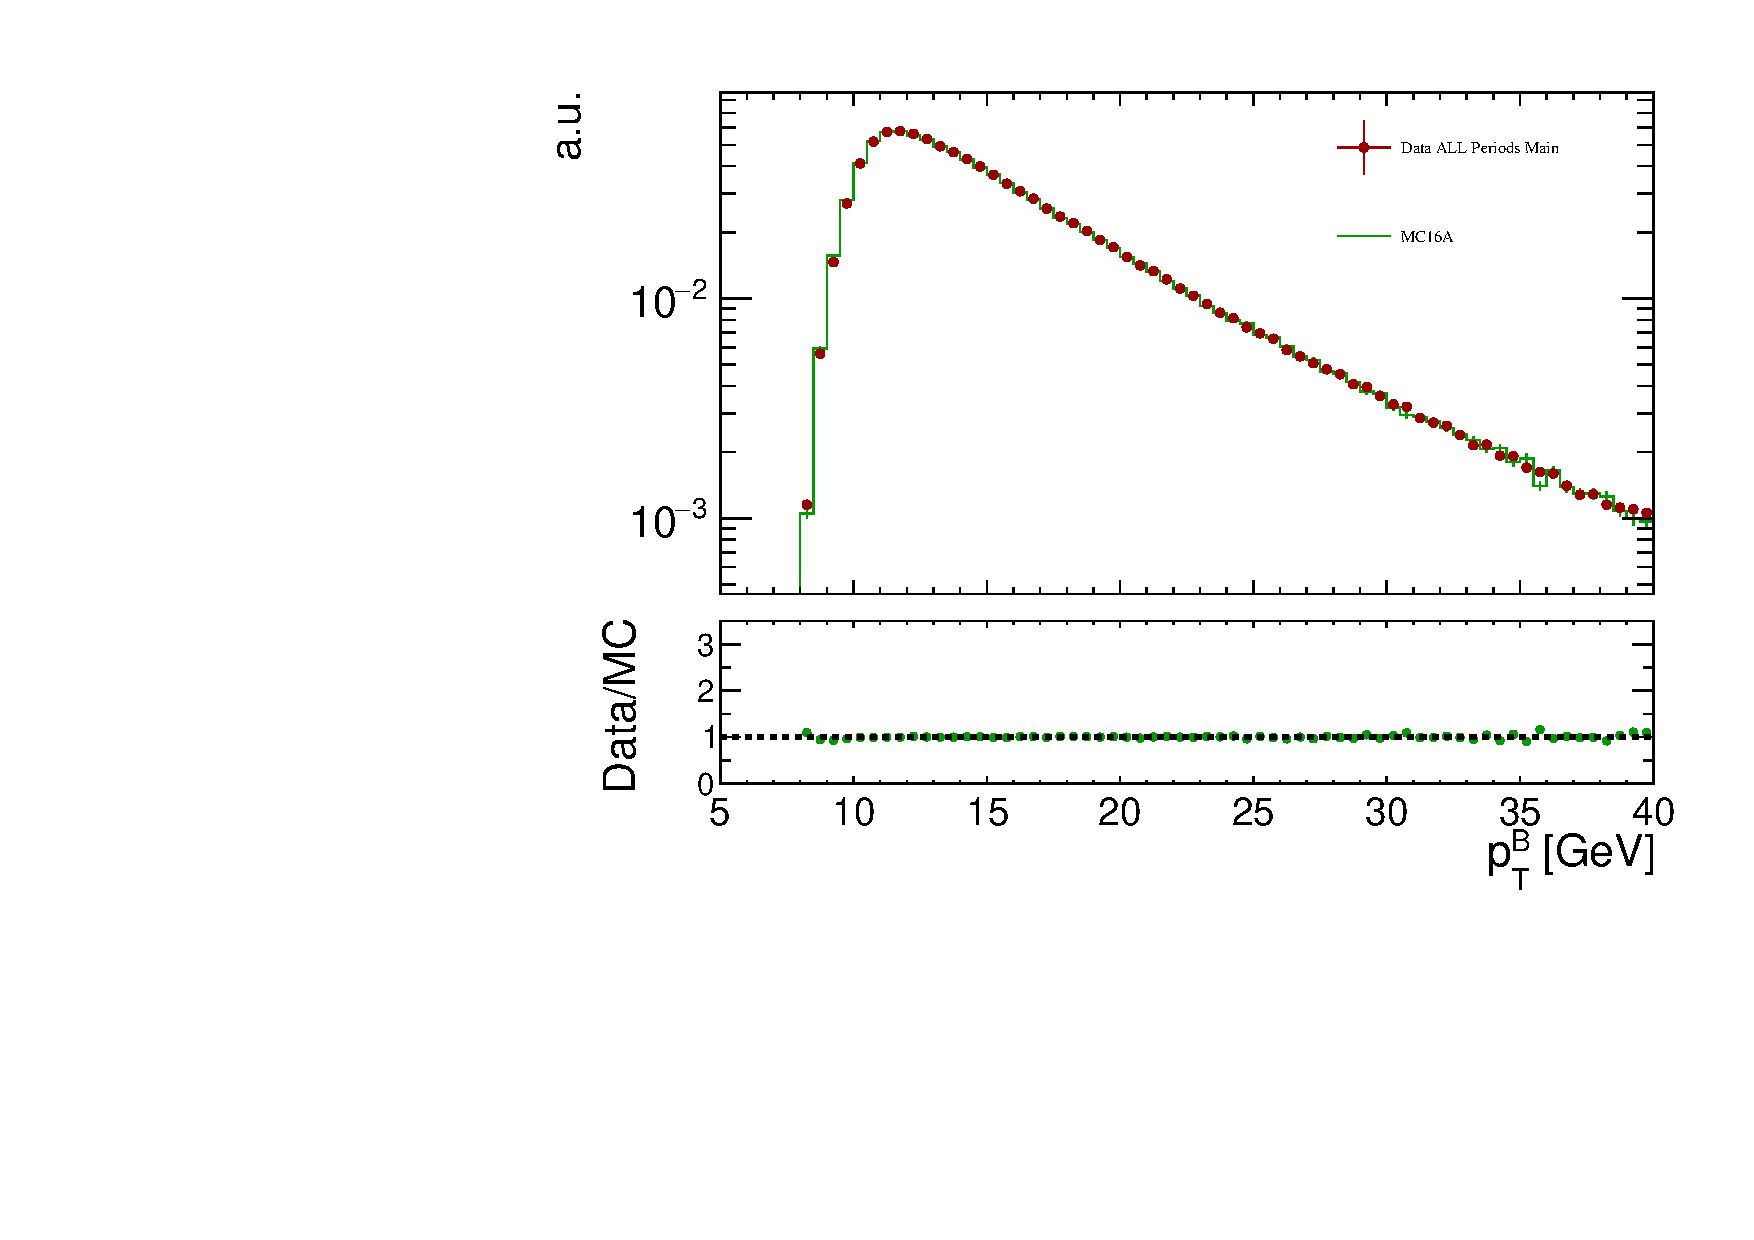
\includegraphics[width=0.52\textwidth]{figures/InternalNote_DataMCComparison/comp/B_pT_dt_mcXs.pdf}
\hspace*{-0.3cm}
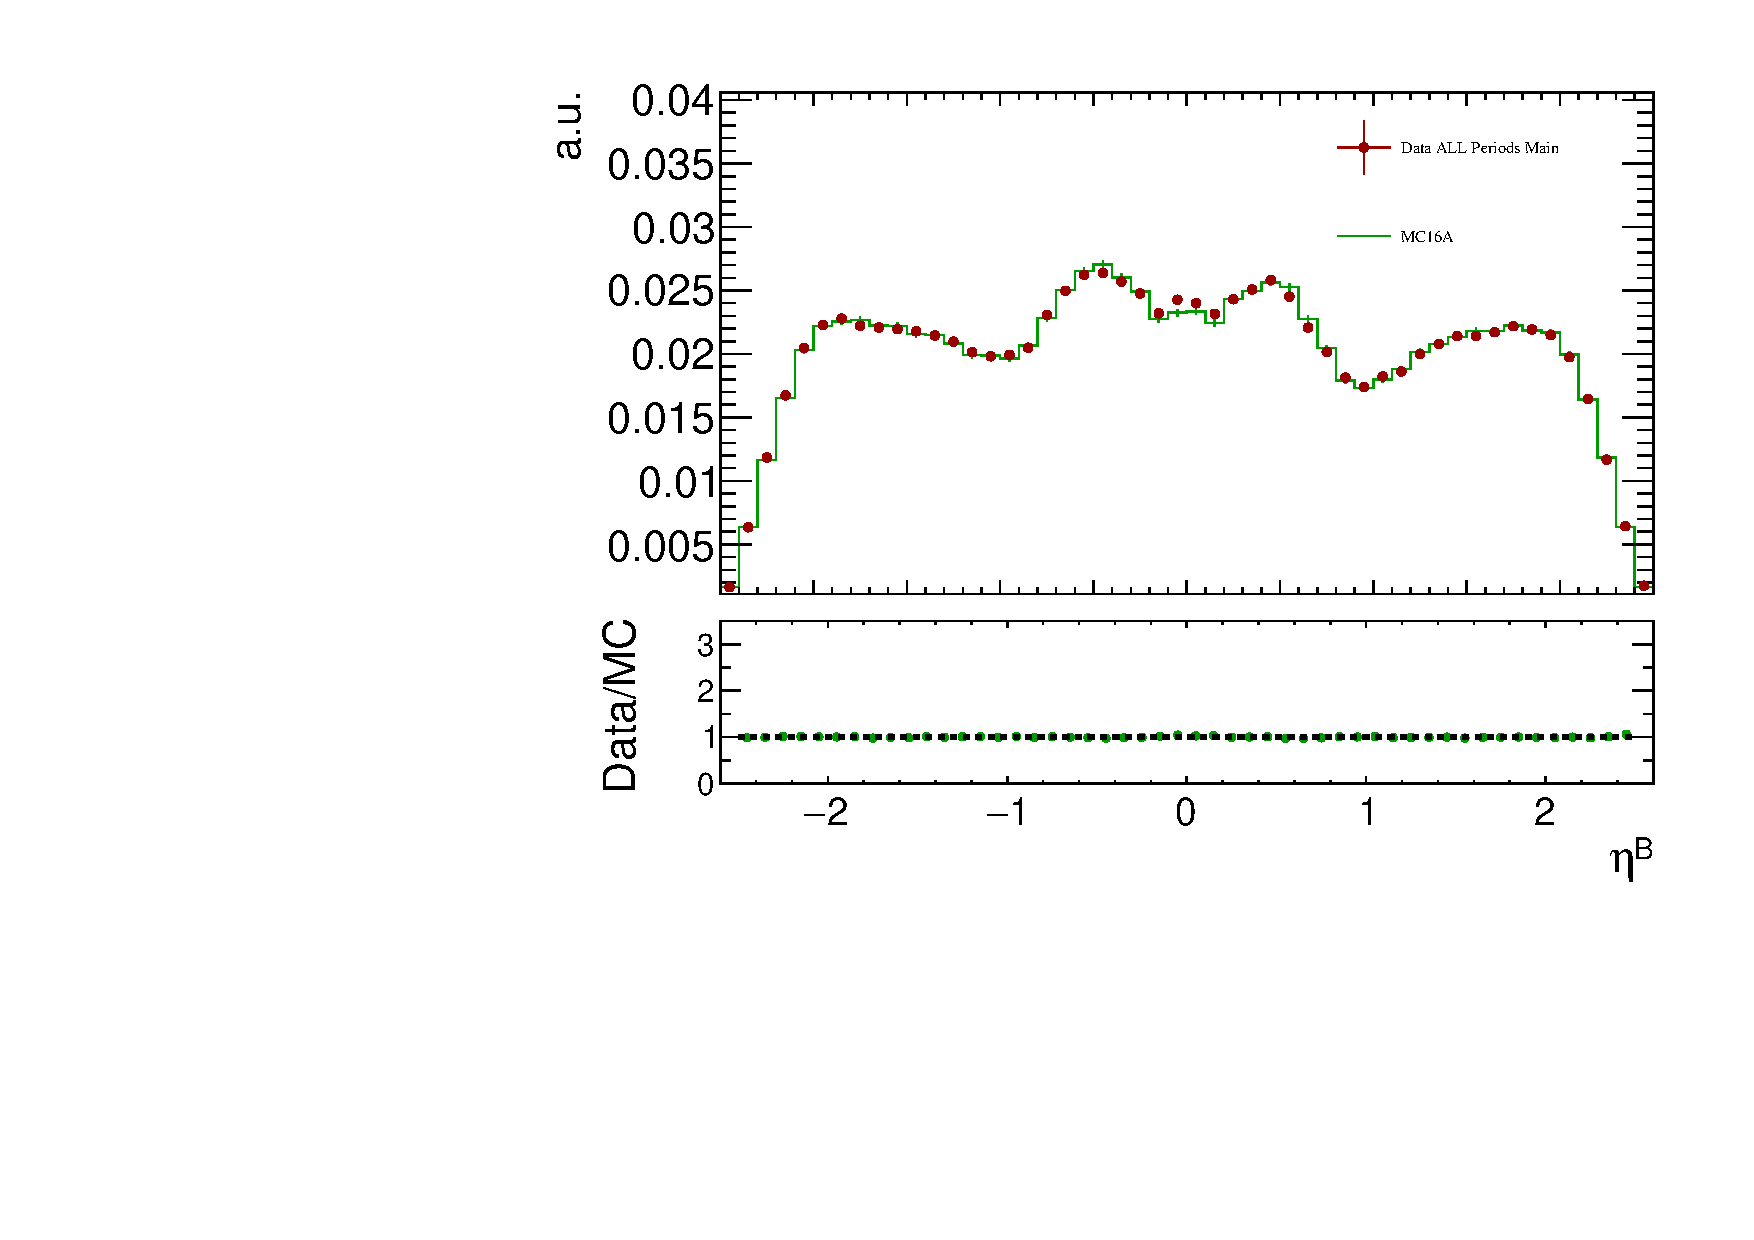
\includegraphics[width=0.47\textwidth]{figures/InternalNote_DataMCComparison/comp/B_eta_dt_mcXs.pdf}
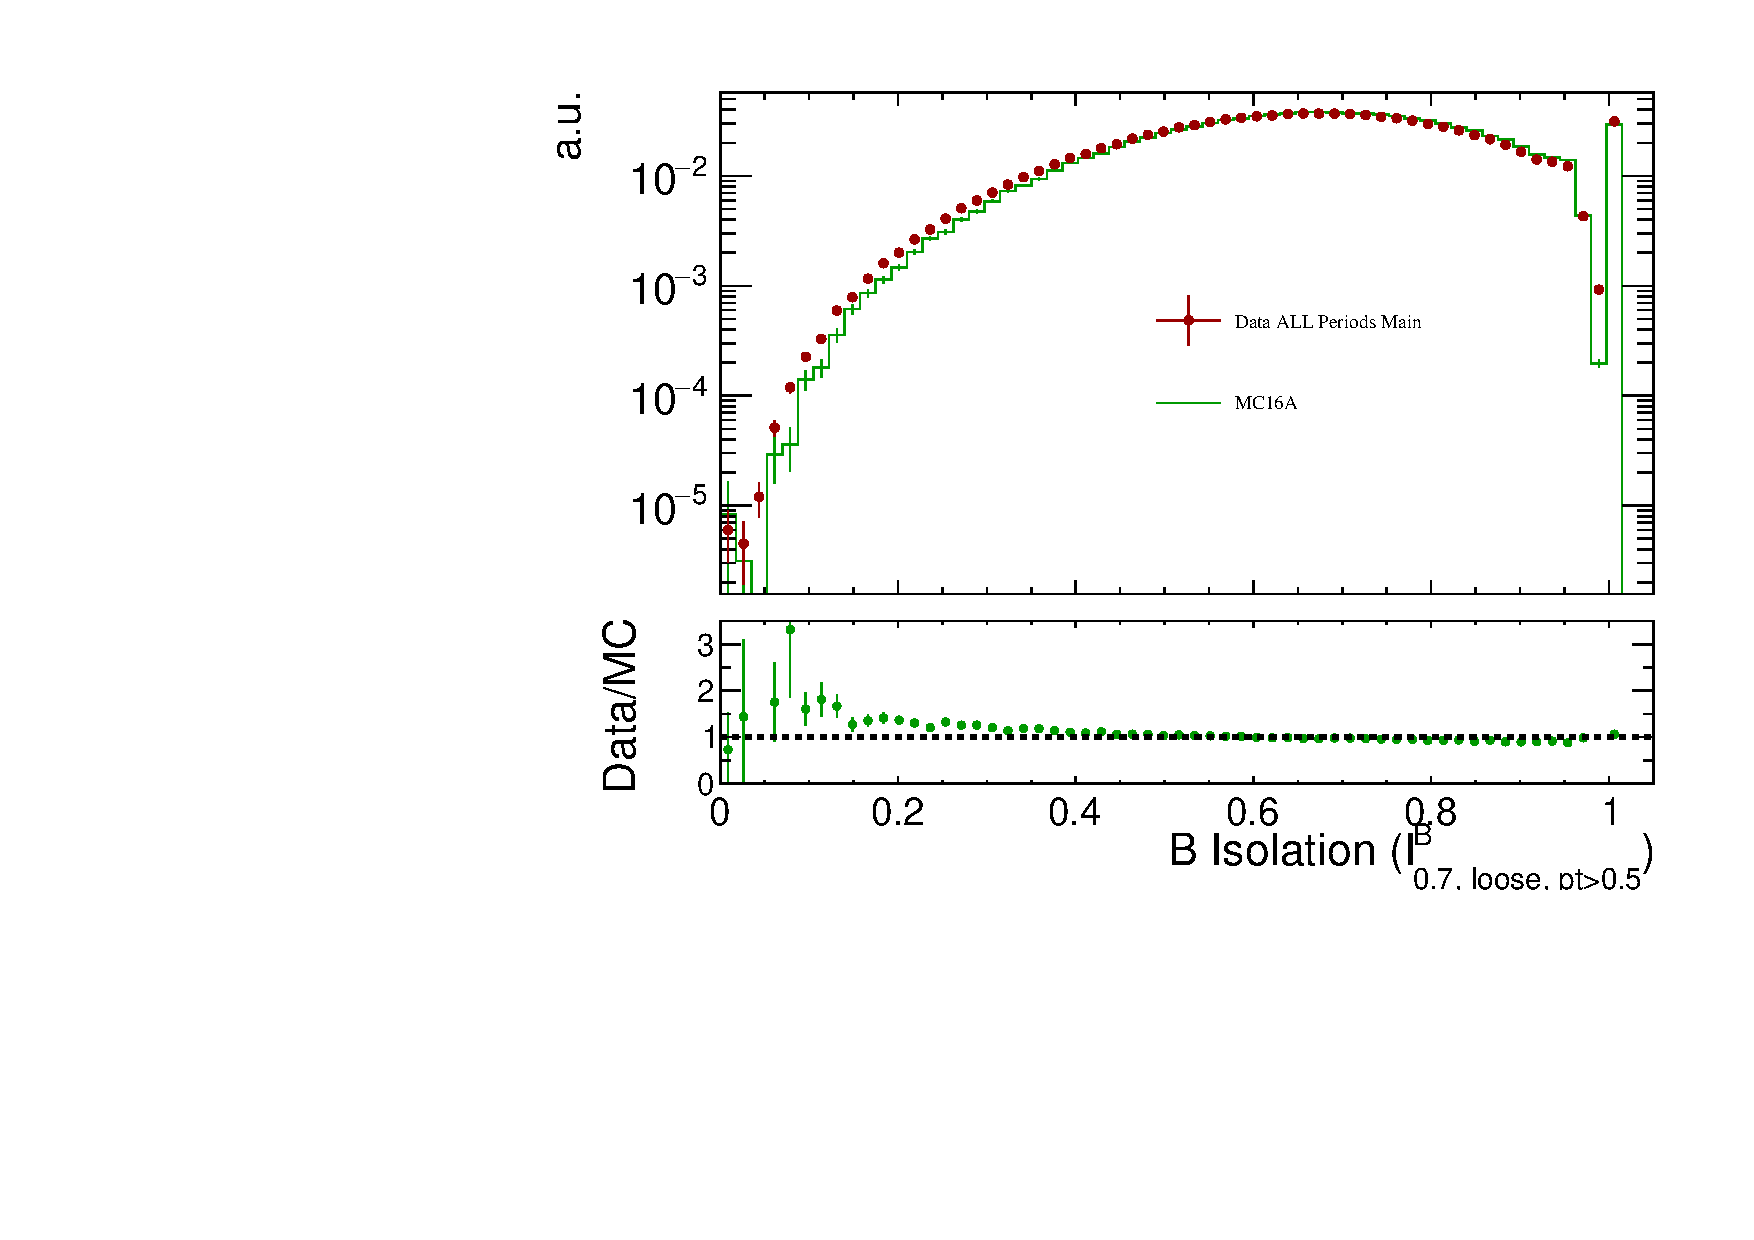
\includegraphics[width=0.52\textwidth]{figures/InternalNote_DataMCComparison/comp/B_iso_7_Chi2_5_LoosePt05_dt_mcXs.pdf}
\caption{Cross-check on the \pt$^B$ and $\eta^B$ distributions of the $J/\psi K$ candidates in data and signal MC.
The red dots correspond to the sideband data during all data taking periods in Run 2 and the green histogram corresponds to the MC $b\bar{b} \to \mu\mu X$ sample. Both histograms are normalised to one.}
\label{fig:xcheckcont}
\end{center}
\end{figure}
%
\begin{figure}[!hbt]
\begin{center}
\hspace*{-0.6cm}
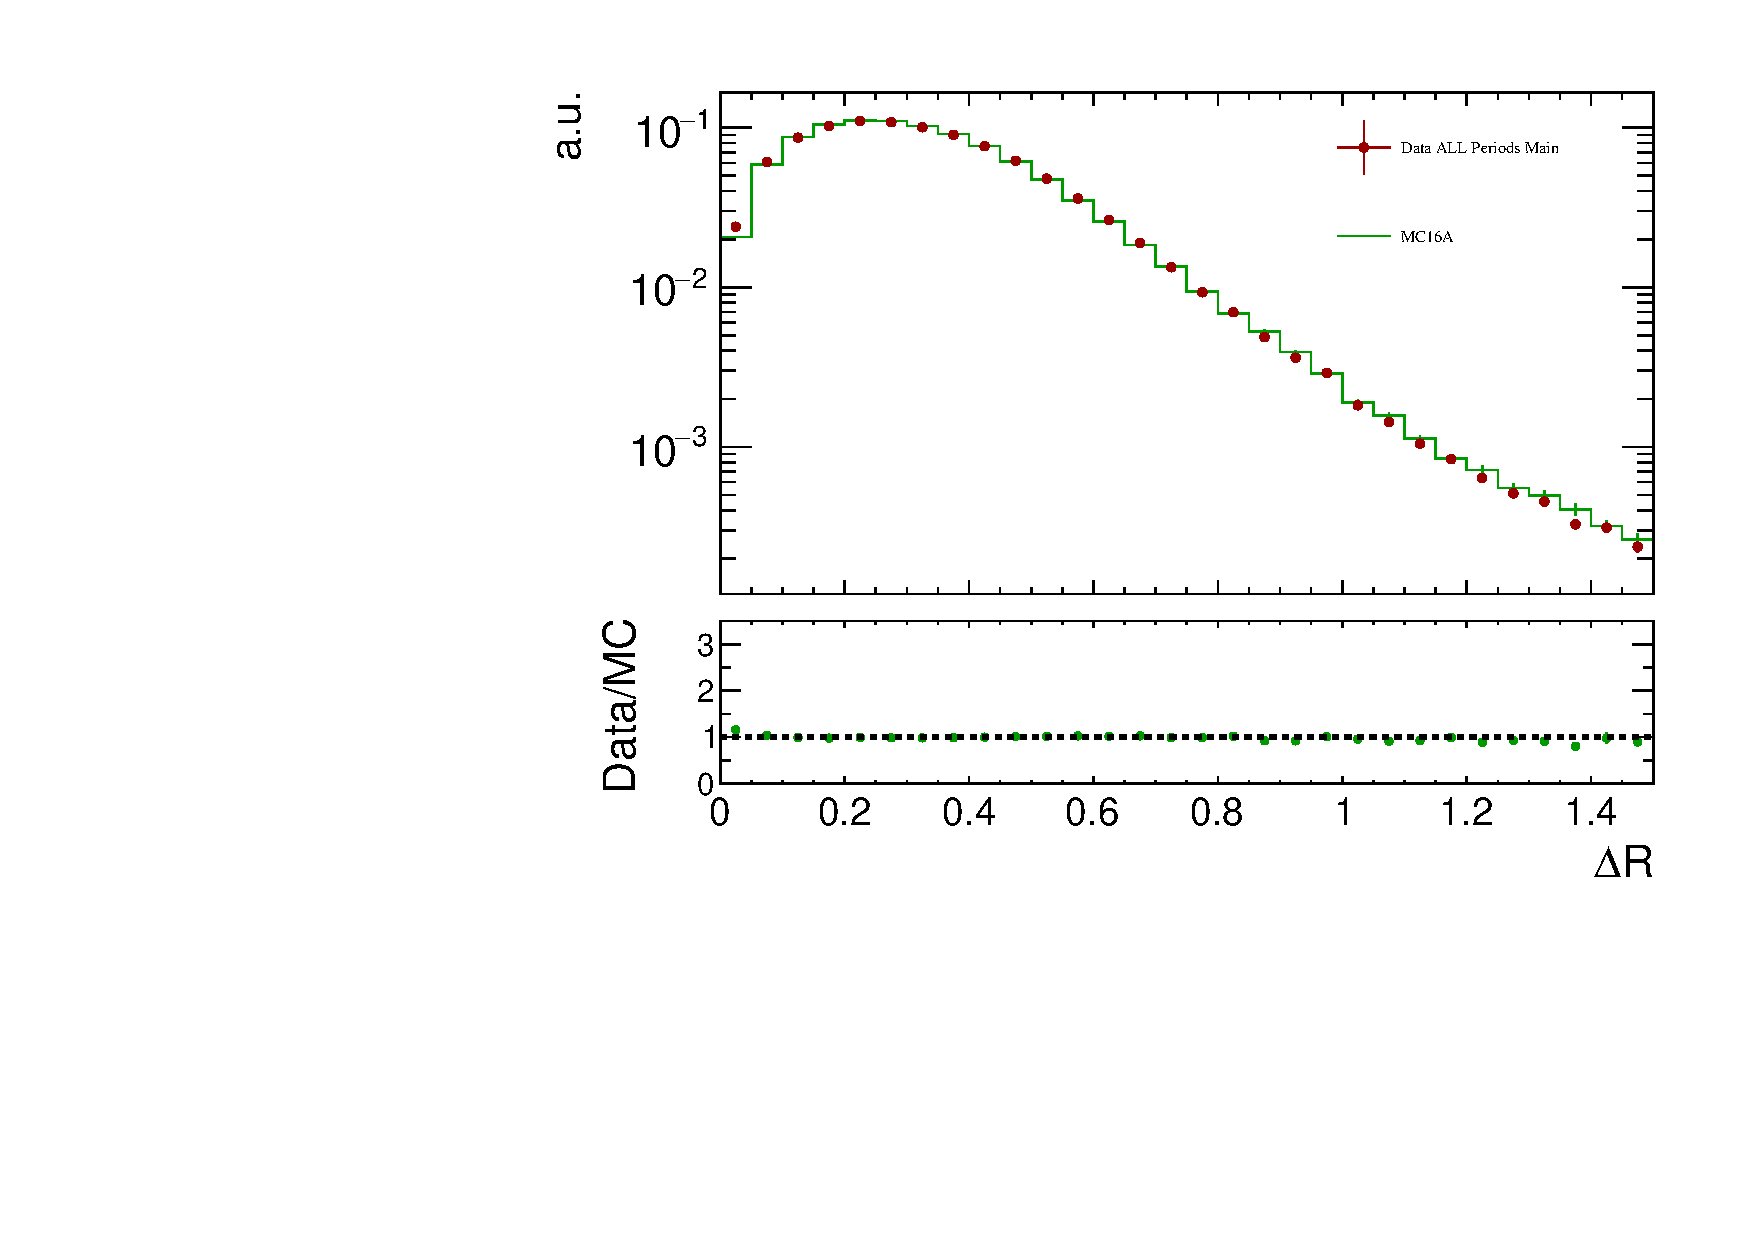
\includegraphics[width=0.52\textwidth]{figures/InternalNote_DataMCComparison/comp/DR_dt_mcXs.pdf}
\hspace*{-0.6cm}
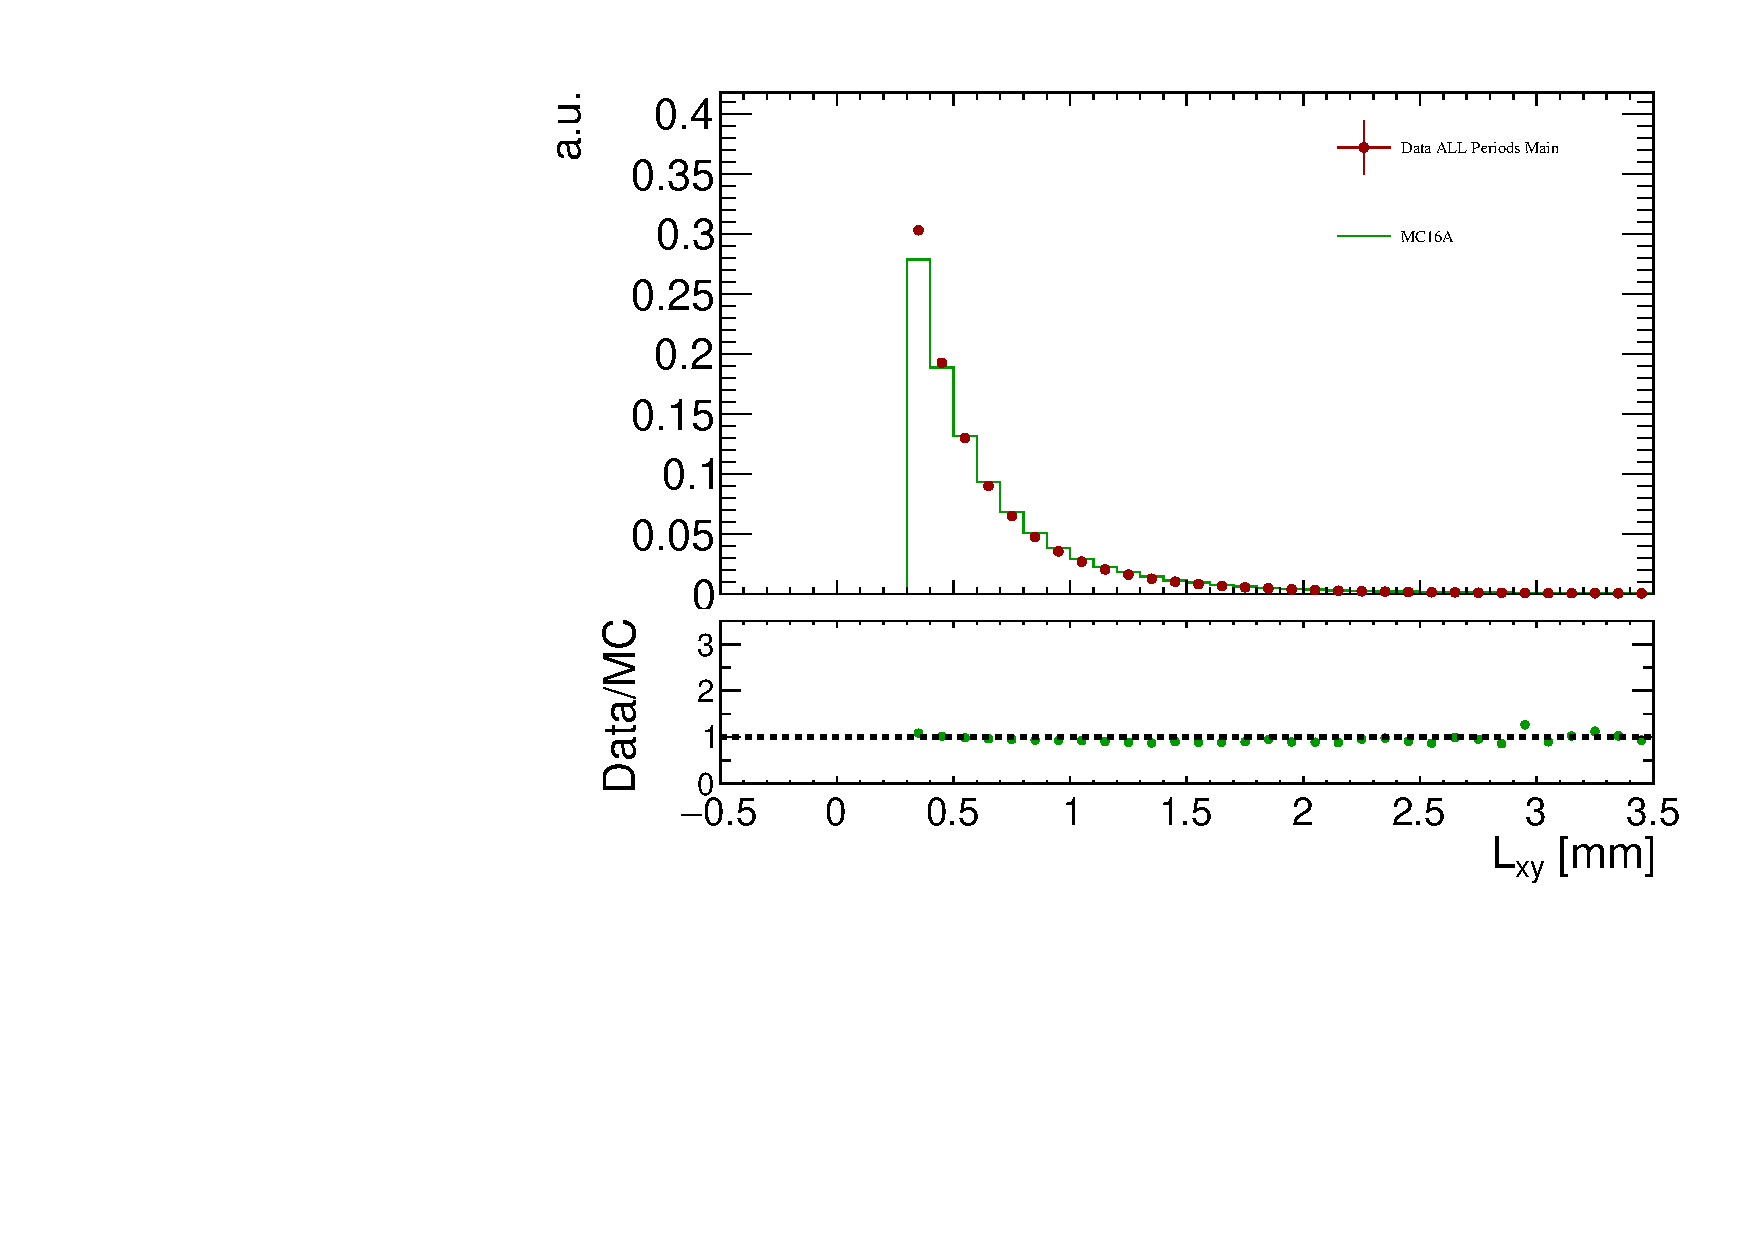
\includegraphics[width=0.52\textwidth]{figures/InternalNote_DataMCComparison/comp/Lxy_dt_mcXs.pdf}\\
\hspace*{-0.6cm}
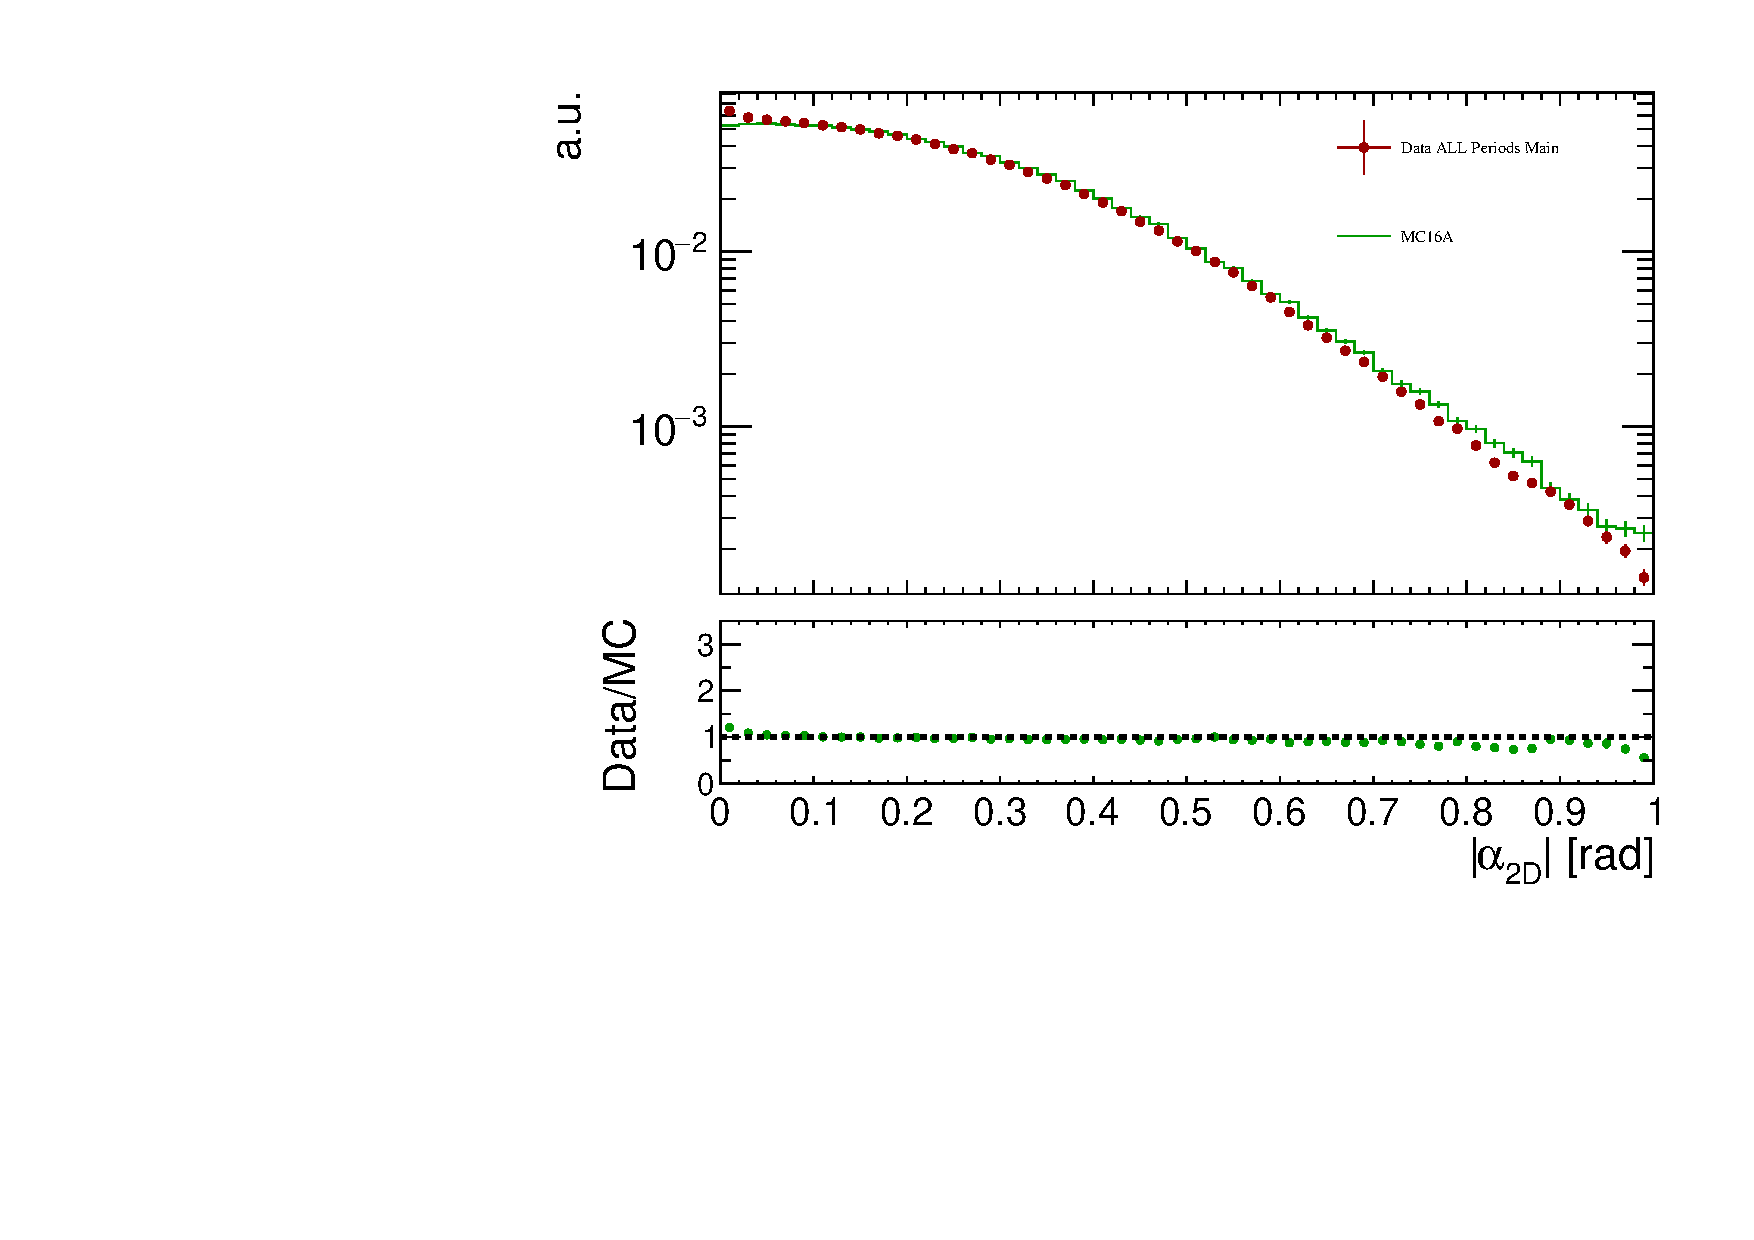
\includegraphics[width=0.52\textwidth]{figures/InternalNote_DataMCComparison/comp/fabs_a_2D__dt_mcXs.pdf}
\hspace*{-0.6cm}
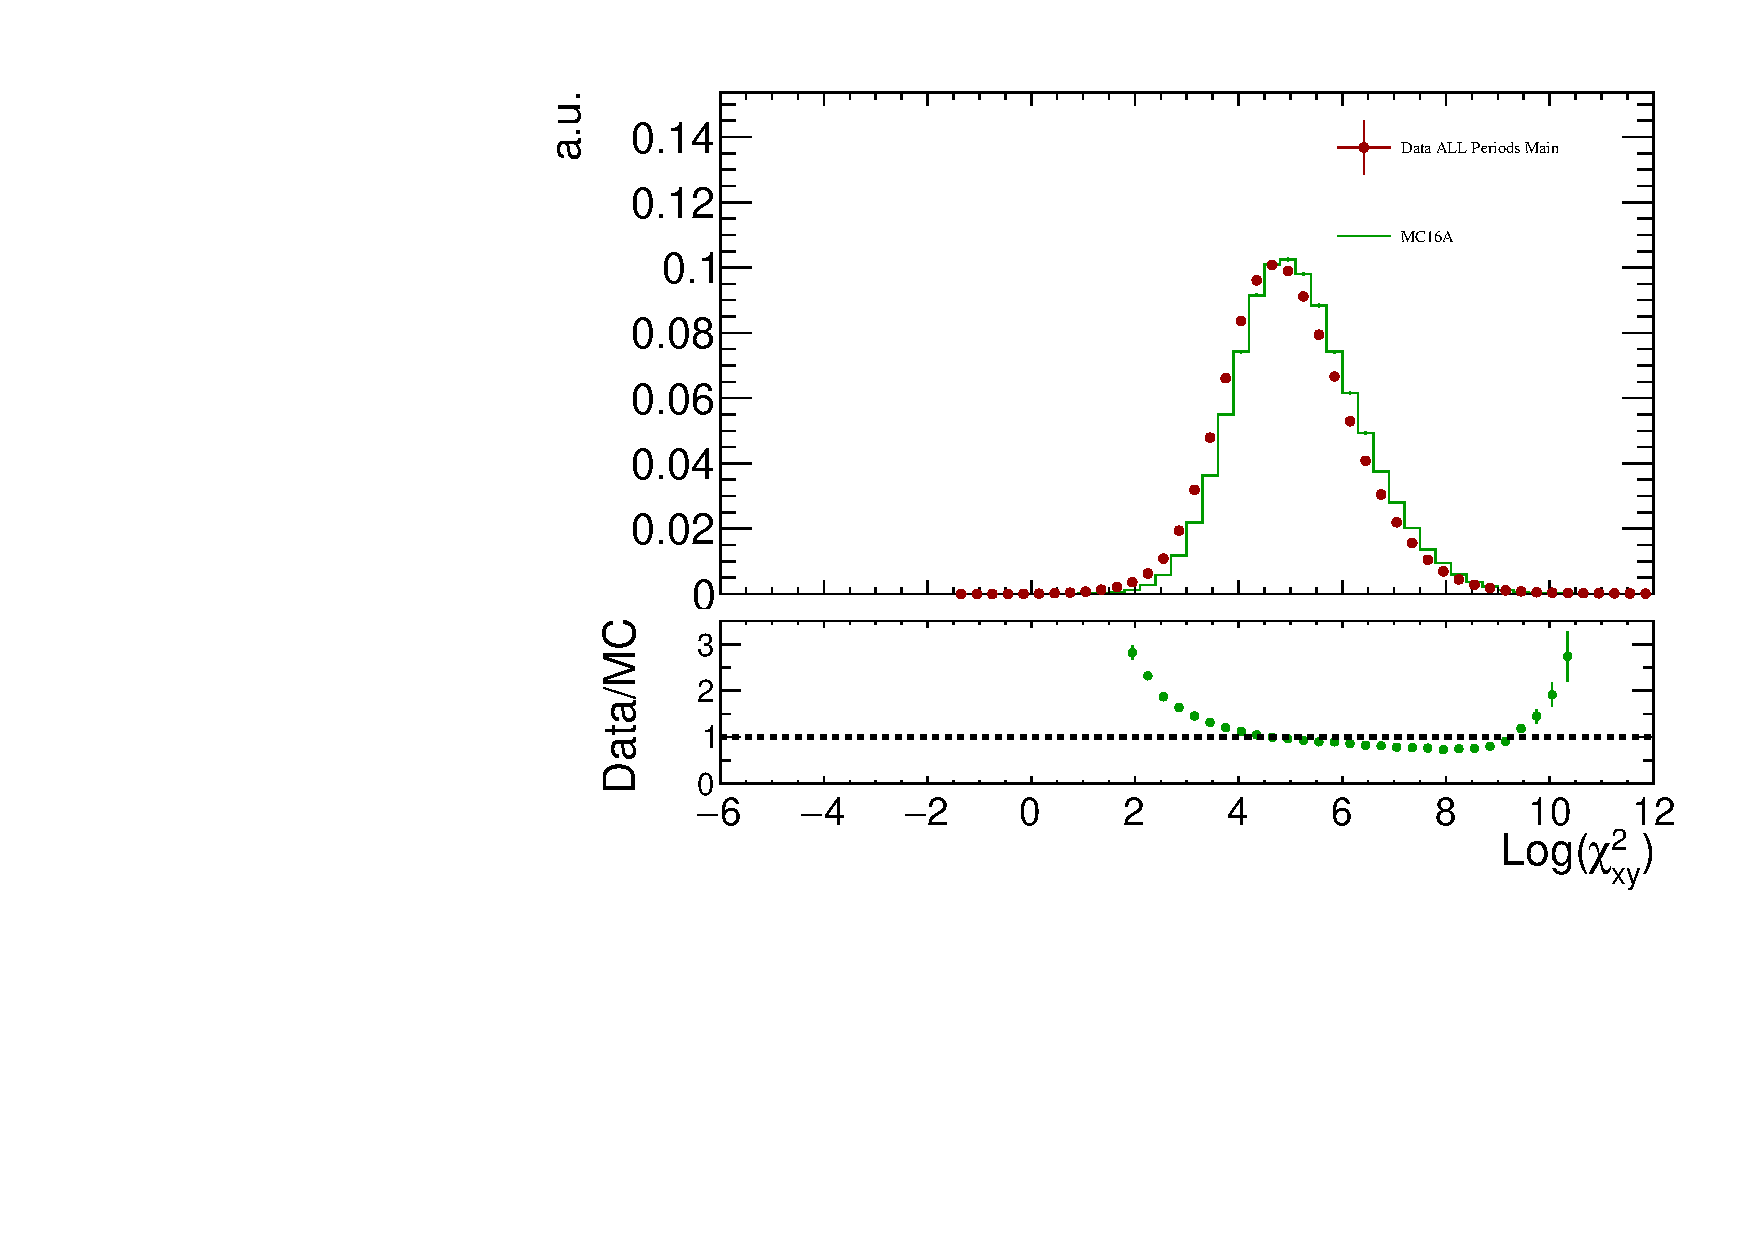
\includegraphics[width=0.52\textwidth]{figures/InternalNote_DataMCComparison/comp/chi2_PVSV_log2D_dt_mcXs.pdf}
\caption{
From left to right, from top to bottom:
Data and signal background MC distributions of the $\Delta R$,
the transverse decay length ($L_{xy}$), $|\alpha_{2D}|$ and
$\chi^{2}_{xy}$ that represents the separation between production
(PV) and decay (SV) vertices.
The green histogram corresponds to the sideband data, while
the red points correspond to the re-weighted signal MC.}
\label{fig:maincompcont}
\end{center}
\end{figure}
  
%\begin{figure}[!hbt]
%\begin{center}
%\hspace*{-0.6cm}
%\includegraphics[width=0.52\textwidth]{eps/contBDT/continuumBDT.pdf}
%%\hspace*{-0.3cm}
%%\includegraphics[width=0.52\textwidth]{eps/contBDT/BvtxLxy_dt_mc_sigFull.pdf}
%\caption{Data and 4-corner background MC distribution of the continuum BDT
%variable. The black dots correspond to the sideband data, while
%the green points correspond to \pt\ and PV re-weighted
%4-corner normalised to the number of data events. The red
%dots show the signal MC distribution as comparison.}
%\label{fig:maincompcontBDT}
%\end{center}
%\end{figure}
  
\subsection{Reference channel as control sample for signal: \BpKpJpsi}
\label{sec:compsig}

The MC sample for the reference channel \BpKpJpsi\ is used to compare
the signal MC shapes with the collision data. The MC sample is
\yel[t.b.d. - currently brute-force approach]{re-weighted with the GLC and the DDW} described in Secs.~\ref{sec:glc}
and~\ref{sec:ddw}. For the data sample, the shape of the background
distribution for each discriminating variable is estimated using the
events falling into the left ($5080\MeV<m_{\Jpsi K^{\pm}}<5180\MeV$)
and the right ($5380\MeV<m_{\Jpsi K^{\pm}}<5480\MeV$) sidebands.

The left sideband contains also a fraction of mis-reconstructed decays
that behave signal-like from the point of view of the discriminating
variables. We re-weight the left sideband considering the combinatorial
contribution only: the net effect is that some of the signal will be
also subtracted as mis-reconstructed $B$ events.~\footnote{From the
binned fit we extract the number of combinatorial background events
in the left and in the right sidebands (let's call them C and D) and
also in the signal region (let's call it A).
Then we normalise the sideband distributions to A/(C+D), effectively
subtracting the right amount of combinatorial background feeding into
the signal region.}
It is proven that the mis-reconstructed events have the same shape as
the signal in the discriminating variables considered, so no distortion
of the signal shapes is created by this subtraction.

\begin{figure}[!ht]
\begin{center}
\hspace*{-0.6cm}
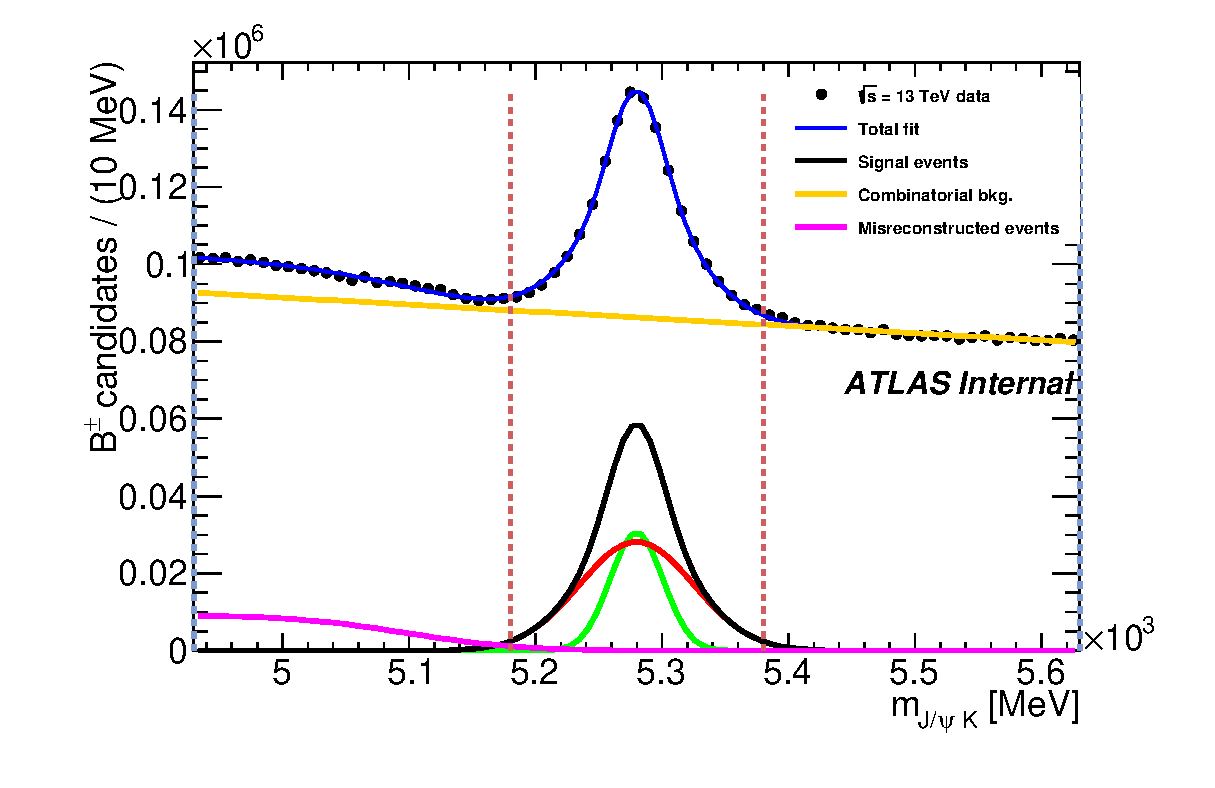
\includegraphics[width=0.47\textwidth]{figures/InternalNote_DataMCComparison/Bp/bplusbinnedfit.eps}
\caption{
Fit to the invariant mass distributions of \BpKpJpsi\ events.}
\label{fig:bplusbinned}
\end{center}
\end{figure}
%
\begin{figure}[!htb]
\begin{center}
\hspace*{-0.6cm}
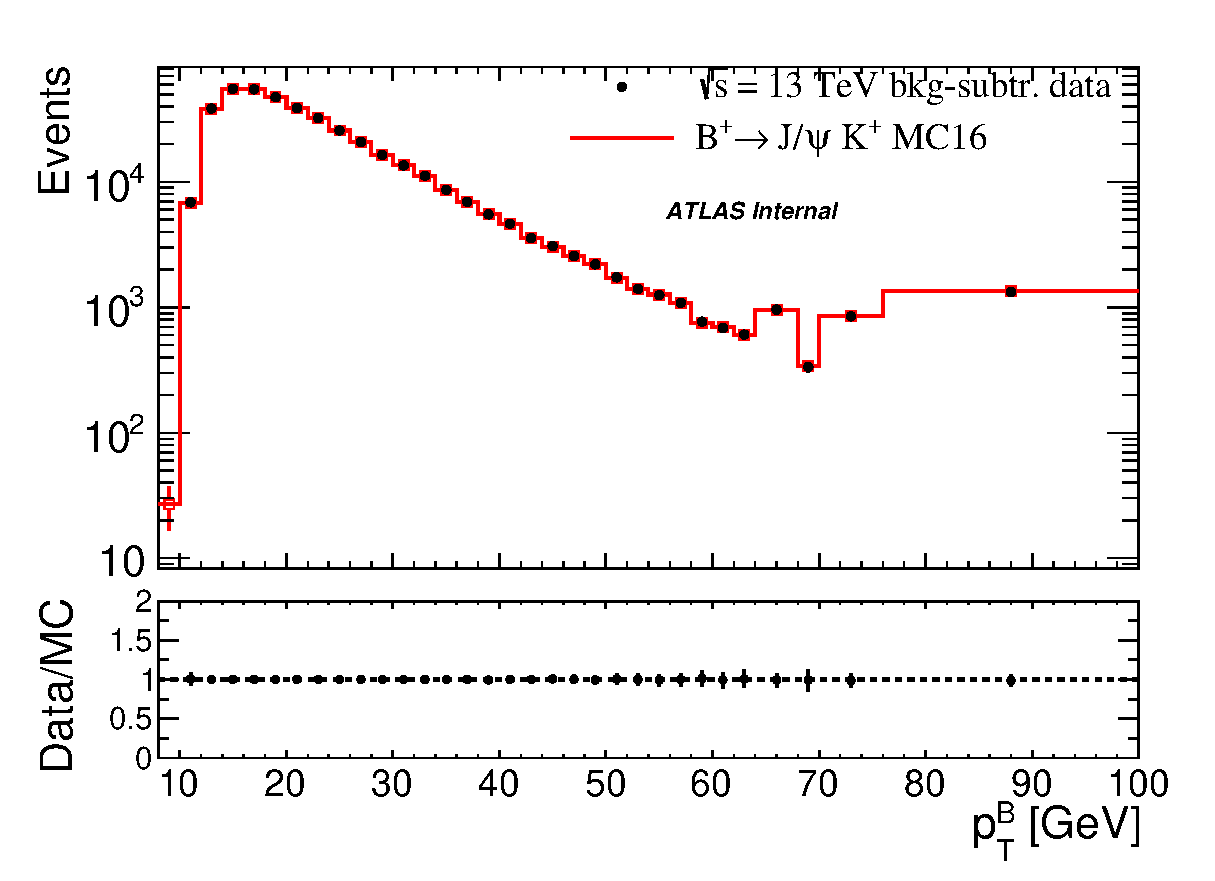
\includegraphics[width=0.52\textwidth]{figures/InternalNote_DataMCComparison/Bp/bplus_pT.eps}
\hspace*{-0.6cm}
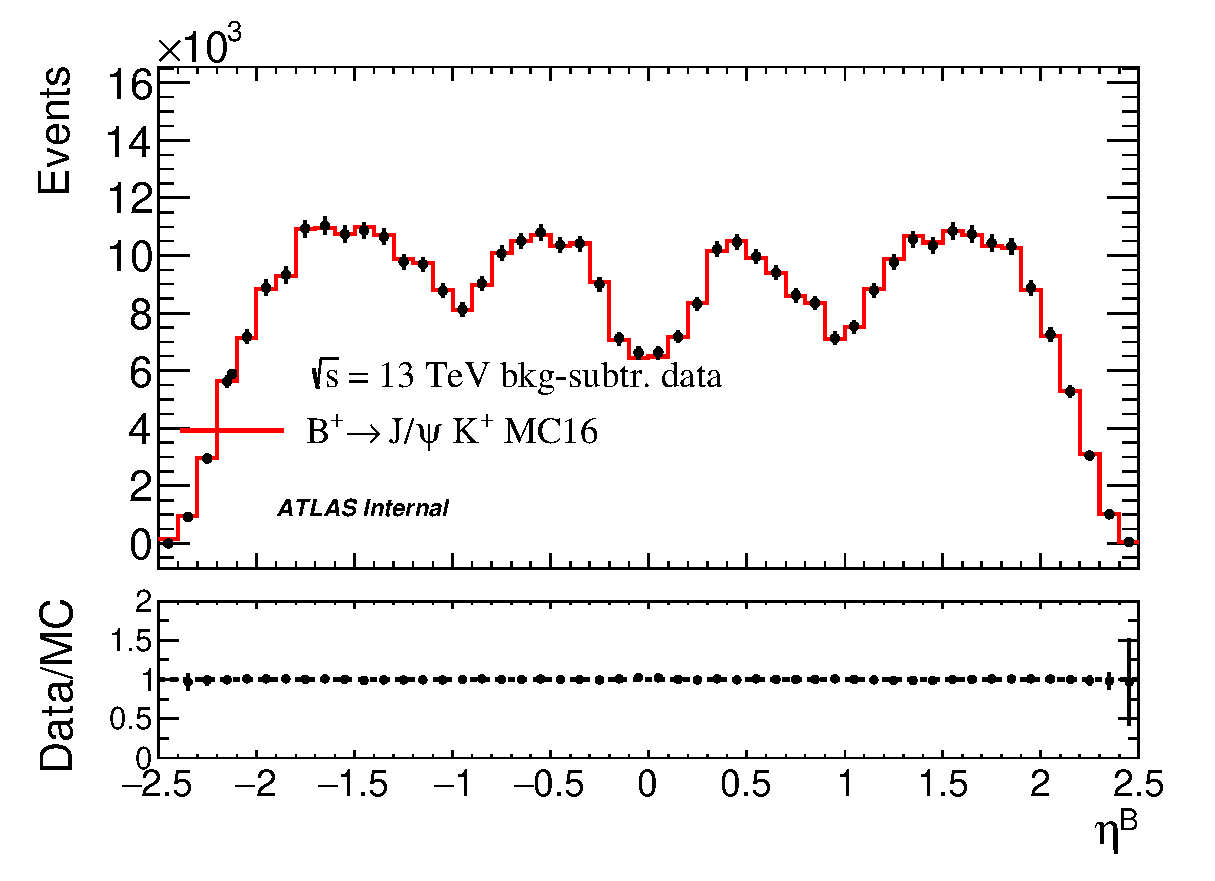
\includegraphics[width=0.52\textwidth]{figures/InternalNote_DataMCComparison/Bp/bplus_eta.eps}
\caption{Cross-check on the \pt$^B$ and $\eta^B$ distributions of
the $J/\psi K$ candidates in data and signal MC.
The black dots correspond to the sideband subtracted data, while 
the red histograms correspond to reweighted MC 
normalised to the number of data events.}
\label{fig:xcheckcompBp}
\end{center}
\end{figure}
%
\begin{figure}[!b]
\begin{center}
\hspace*{-0.4cm}
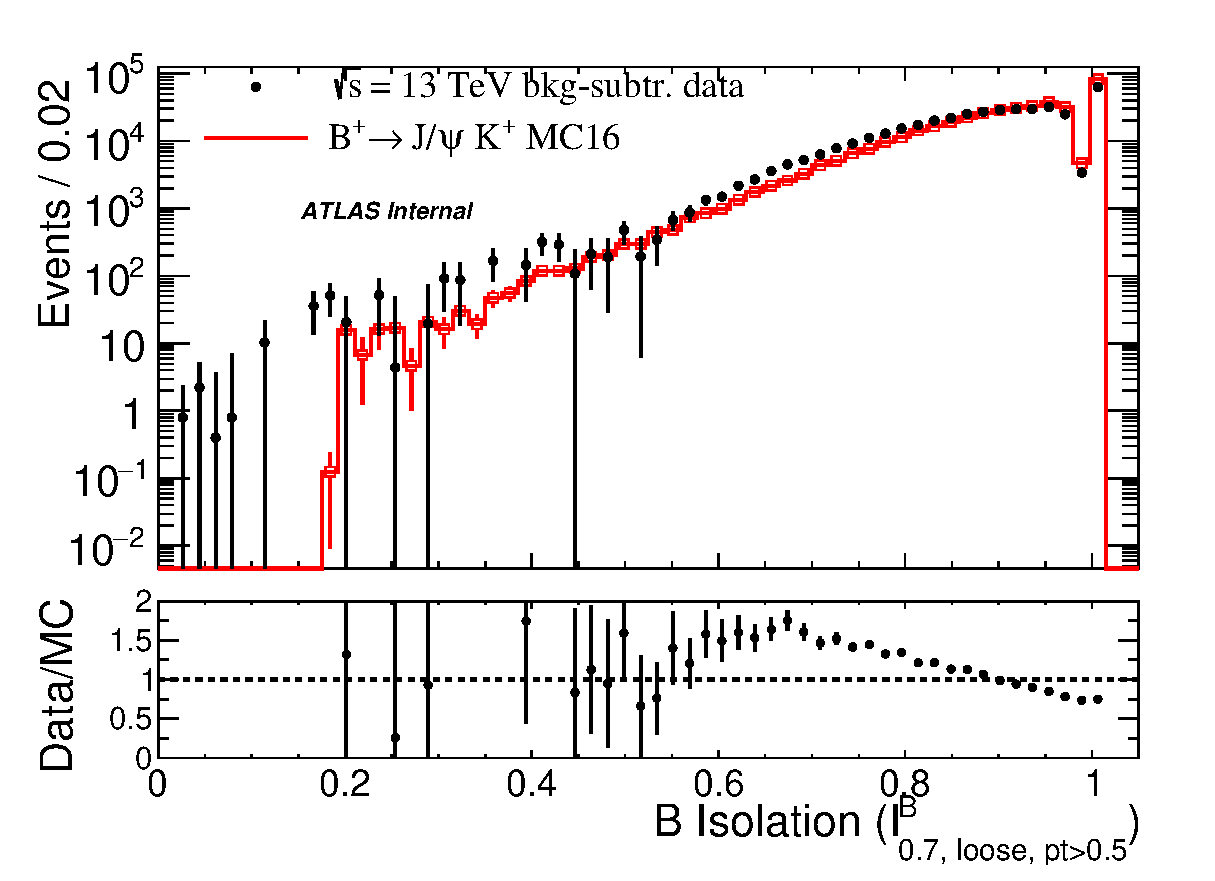
\includegraphics[width=0.47\textwidth]{figures/InternalNote_DataMCComparison/Bp/bplus_iso.eps}
\hspace*{-0.4cm}
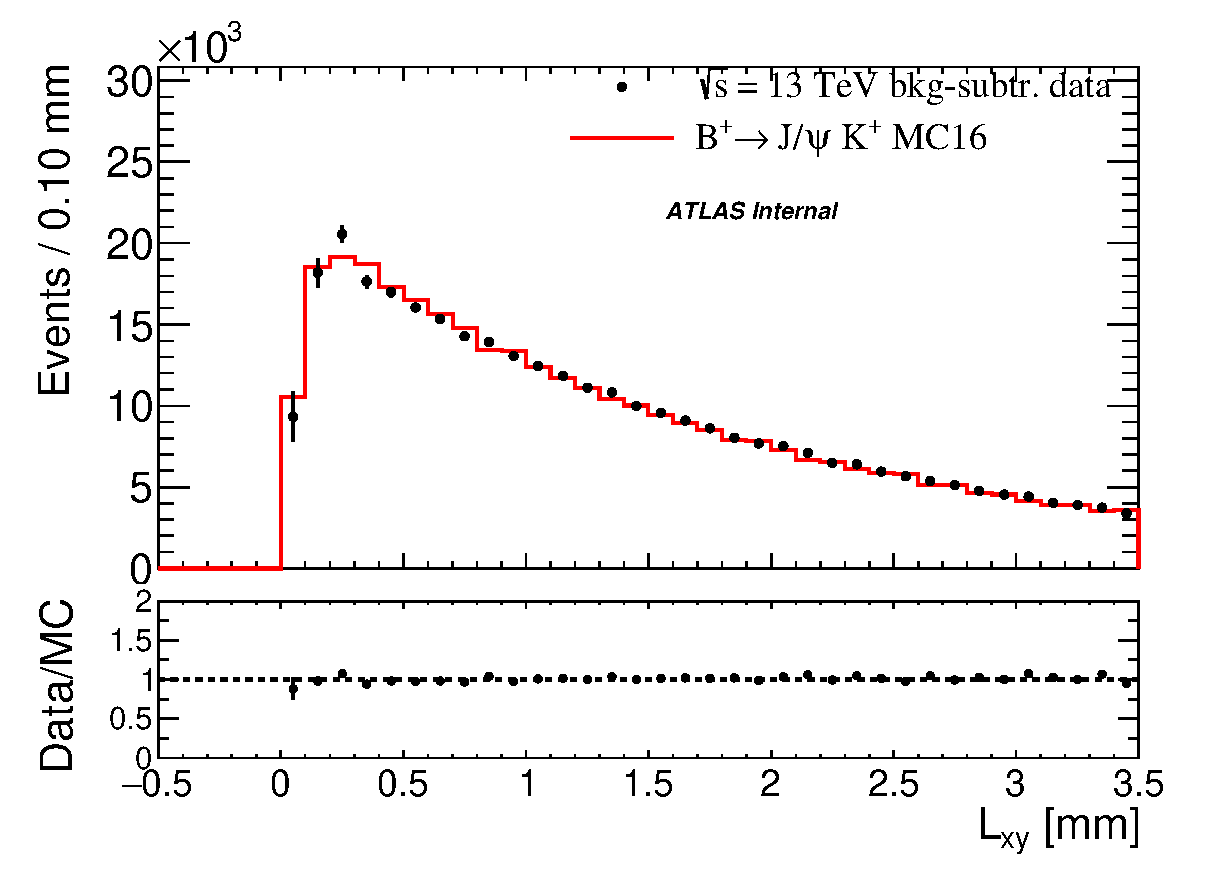
\includegraphics[width=0.47\textwidth]{figures/InternalNote_DataMCComparison/Bp/bplus_Lxy.eps}\\
\hspace*{-0.4cm}
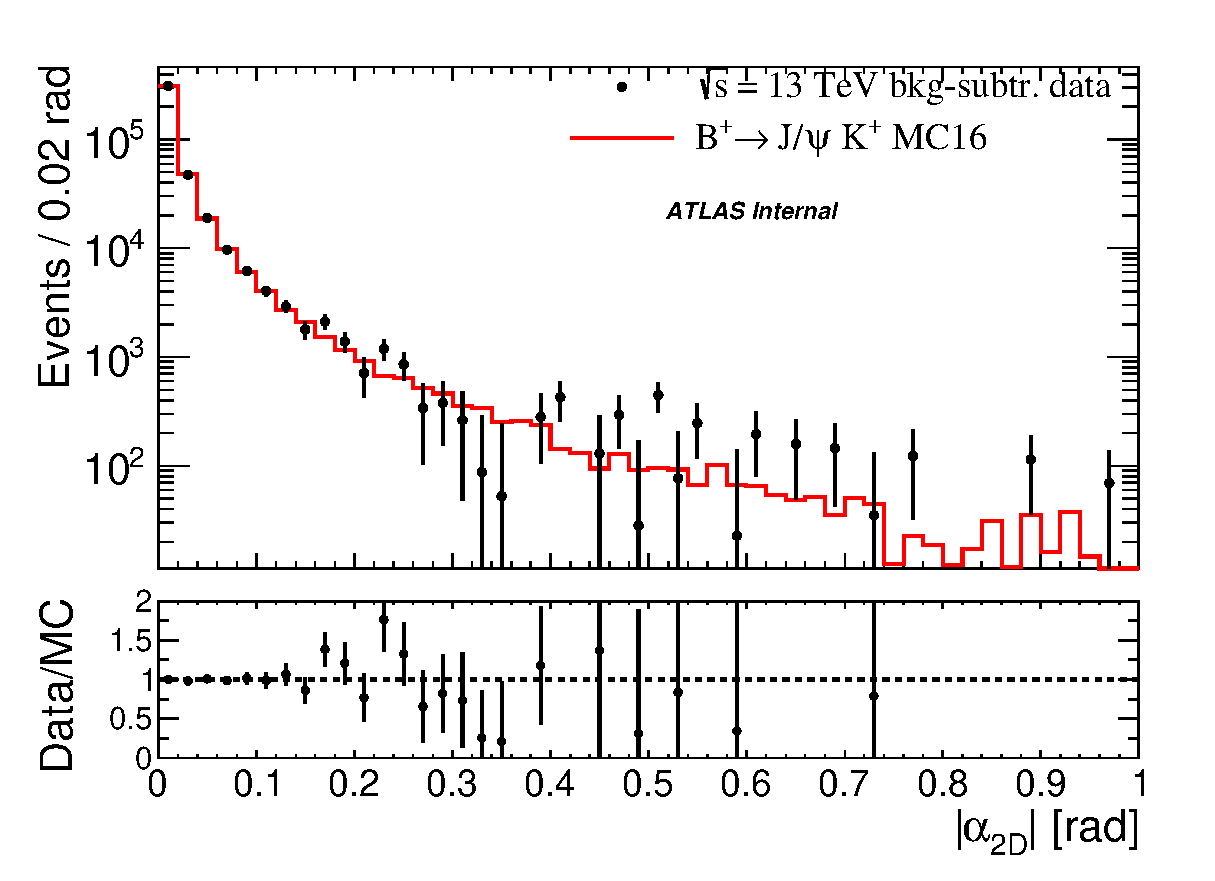
\includegraphics[width=0.47\textwidth]{figures/InternalNote_DataMCComparison/Bp/bplus_a2D.eps}
\hspace*{-0.4cm}
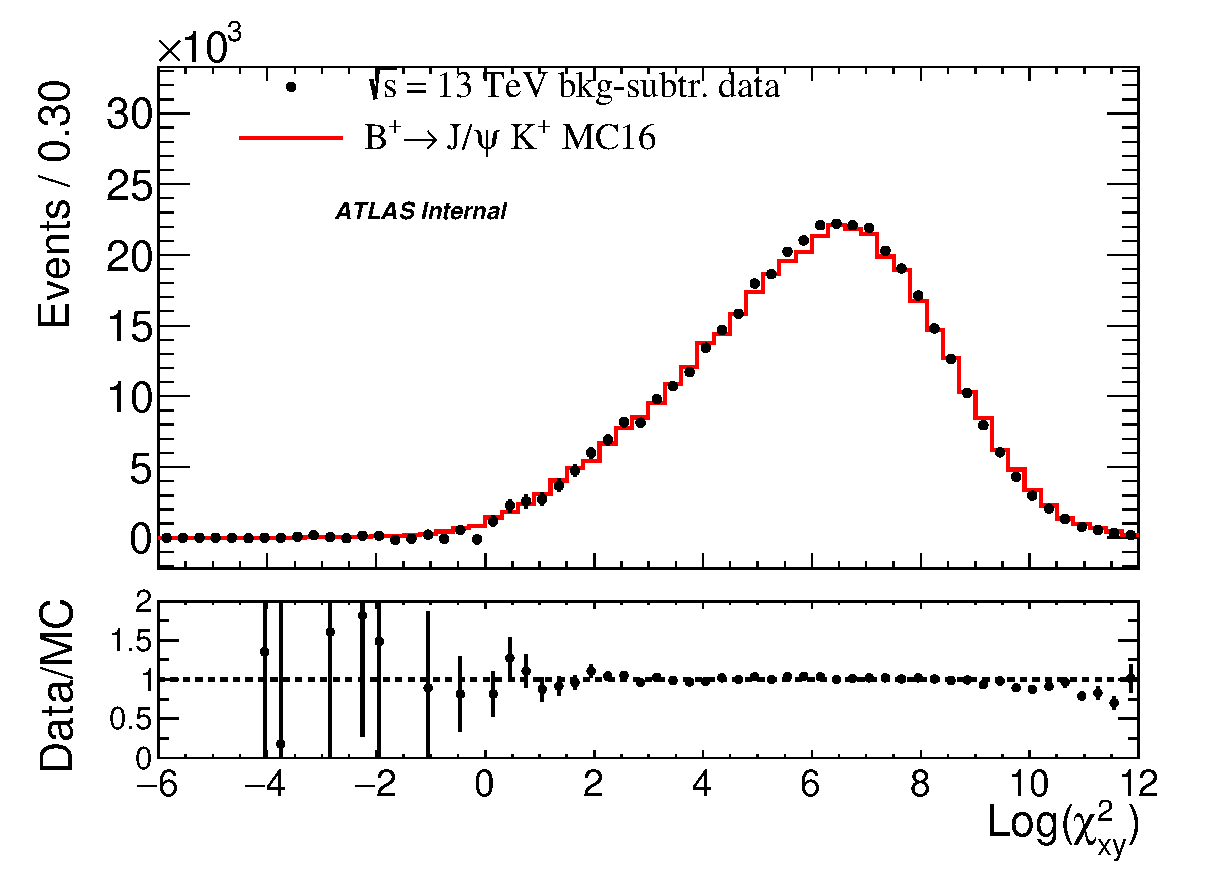
\includegraphics[width=0.47\textwidth]{figures/InternalNote_DataMCComparison/Bp/bplus_chi2PVSV.eps}
\caption{{\it{From left to right, from top to bottom}}: 
Data and signal MC distributions in \BpKpJpsi\ events for the $B$ isolation variable, 
the transverse decay length ($L_{xy}$), $|\alpha_{2D}|$ and 
$\chi^{2}_{xy}$ that represents the separation between production
(PV) and decay (SV) vertices.
The black dots correspond to the sideband subtracted data, while 
the red points correspond to reweighted MC
normalised to the number of data events.}
\label{fig:maincompBp}
\end{center}
\end{figure}
%
\begin{figure}[!b]
\begin{center}
\hspace*{-0.4cm}
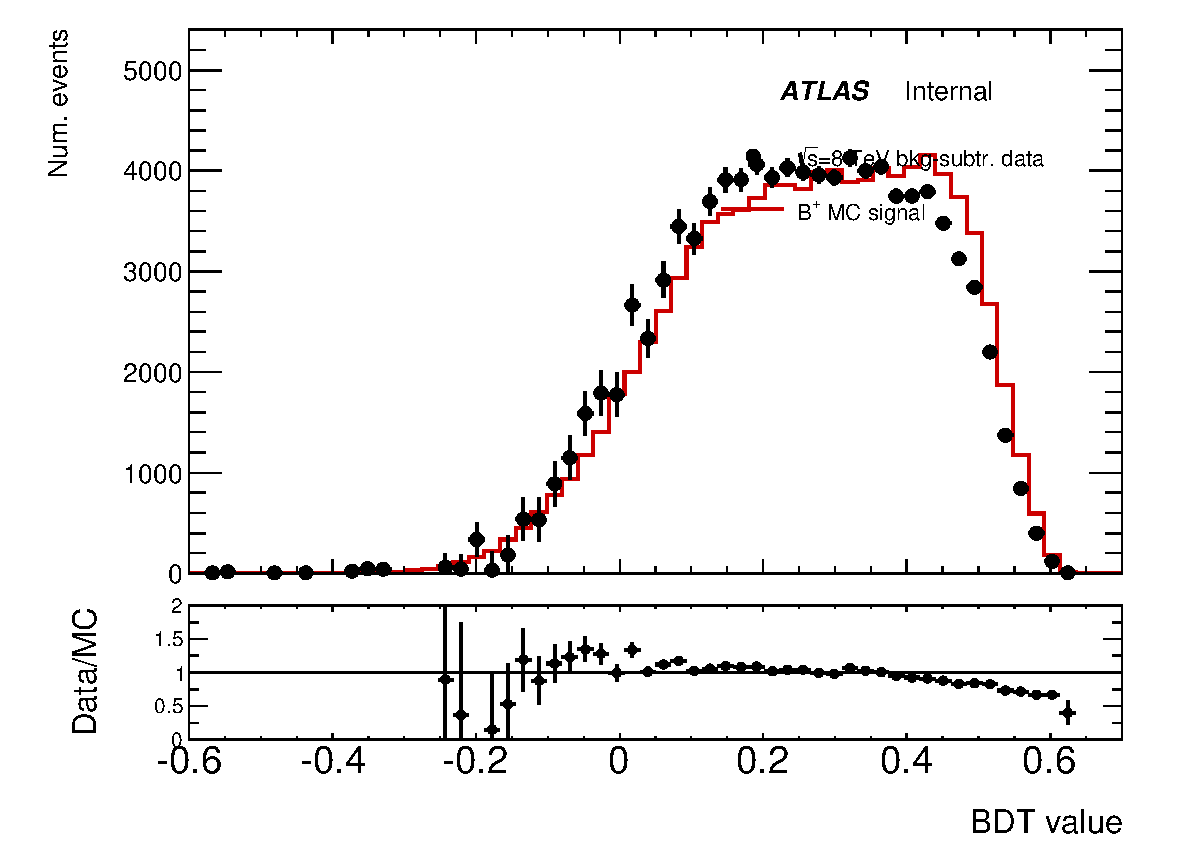
\includegraphics[width=0.47\textwidth]{figures/InternalNote_DataMCComparison/compRun1/Bp/bplus_BDT.pdf}
\hspace*{-0.4cm}
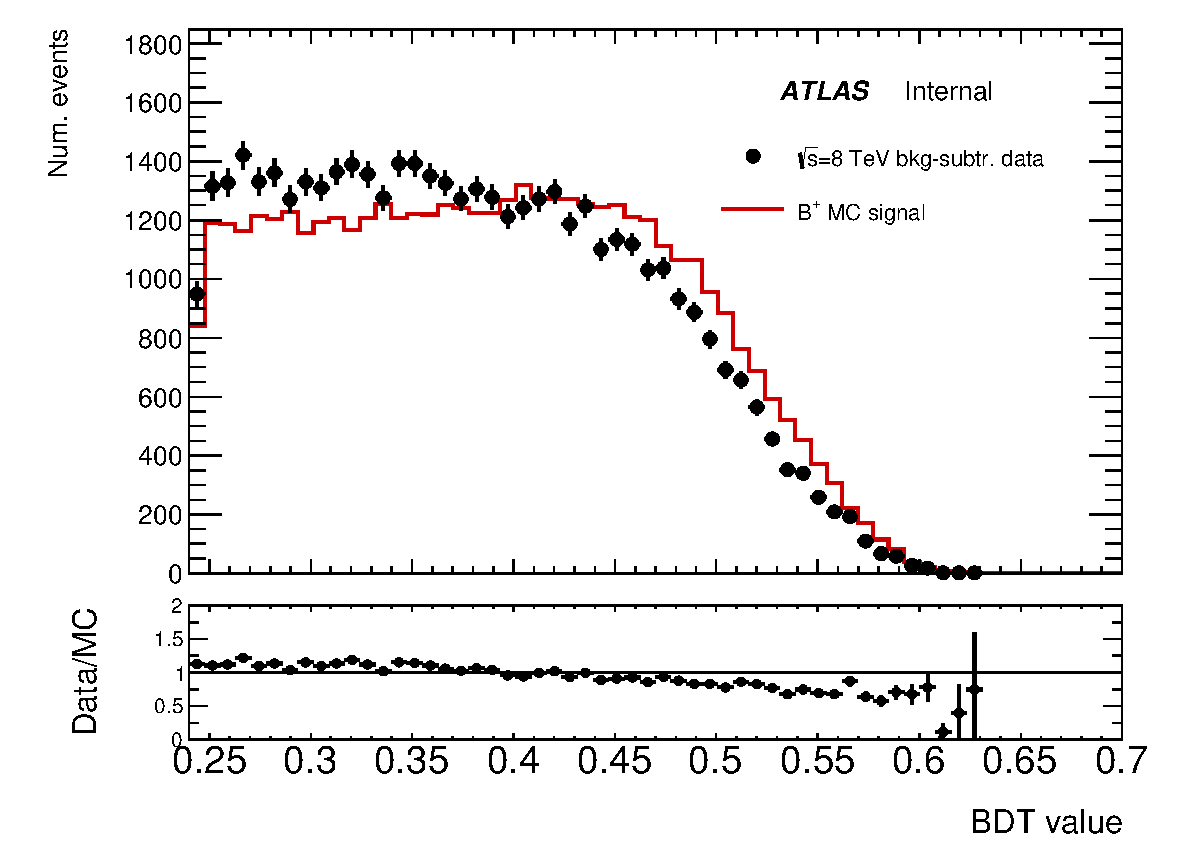
\includegraphics[width=0.47\textwidth]{figures/InternalNote_DataMCComparison/compRun1/Bp/bplus_BDTzoomed.pdf}
\caption{\textbf{Run 1 result, t.b.u.!}Data and signal MC distribution in \BpKpJpsi\ events for the
continuum BDT variable.
The black dots correspond to the sideband subtracted data, while 
the red points correspond to reweighted MC normalised to the number
of data events. The left plot shows the same distribution zoomed
in the region of interest of the analysis.}
\label{fig:maincompBpBDT}
\end{center}
\end{figure}
%
The shape from the rescaled sideband events is subtracted statistically
from the signal region. The number of background events
feeding into the signal region is obtained by a binned
maximum likelihood fit to the mass distribution.
Figure~\ref{fig:bplusbinned} shows these binned fits to
the mass distributions in the three trigger categories.
The fit model consists of a double Gaussian for
the signal, an error function for the
mis-reconstructed events and an exponential for the continuum
background.
The results of these binned fit analysis are perfectly 
compatible with the unbinned fit described in
Section~\ref{sec:bplus} and used for the yield extraction.

The distributions of \pt{} and $\eta{}$ of the $B$ is rechecked in
figures~\ref{fig:xcheckcompBp}, the distributions of few
discriminating variables are shown in figures~\ref{fig:maincompBp},
and \yel[t.b.d.]{the distribution of the continuum BDT variable is shown in
figure}~\ref{fig:maincompBpBDT}.
The distributions of all the other variables are shown in the
\yel[t.b.d.]{appendix}~\ref{app:comp}.

Typically, except for deviations in individual bins, the overall shapes
of distributions agree well between data and MC. The observed differences
in shape are accounted for as systematics with the procedure described in
Section~\ref{sec:eff}. In addition, the discrepancy seen in the
data-MC comparison of the continuum BDT in the \BpKpJpsi\ events is
assessed and exploited in the evaluation of the efficiency in the
\Bsmumu\ signal in Section~\ref{sec:BDTbineff}.

%For this purpose the differences
%for all discriminating variables are calculated per bin and applied to
%the preselected MC events to estimate the impact on the efficiency evaluation
%for systematic studies.% (Appendix~\ref{sec:MVA}). 


\subsection{Alternate reference channel: \BsJpsiPhi}
\label{sec:compjpsiphi}

The same procedure can be applied on data reconstructed as \BsJpsiPhi.
In this case, a few extra selection cuts are necessary to address the extra
kaon in the final state and to select the $\phi$ mass window:
both kaon \pt\ are requested $>1$~GeV and for the $\phi$ mass we require
$|m_{hh}-m_{\phi}|<15$~MeV. The additional cuts defined in
Section~\ref{sec:addcuts} are also applied.
The invariant mass fits in this case are shown in figure~\ref{fig:jpsiphi}
for the three trigger categories.
The fits are performed binned and a Gaussian PDF is used for the signal shape
while a third order Chebychev is used for the combinatorial background PDF.

%\begin{figure}[!htb]
%\begin{center}
%\includegraphics[width=0.37\textwidth]{figures/InternalNote_DataMCComparison/compRun1/Bs/bsjpsiphi_massfit.pdf}
%\caption{Fit to the invariant mass distributions
%of \BsJpsiPhi\ events.}
%\label{fig:jpsiphi}
%\end{center}
%\end{figure}

\begin{figure}[!htb]
\begin{center}
\hspace*{-1cm}
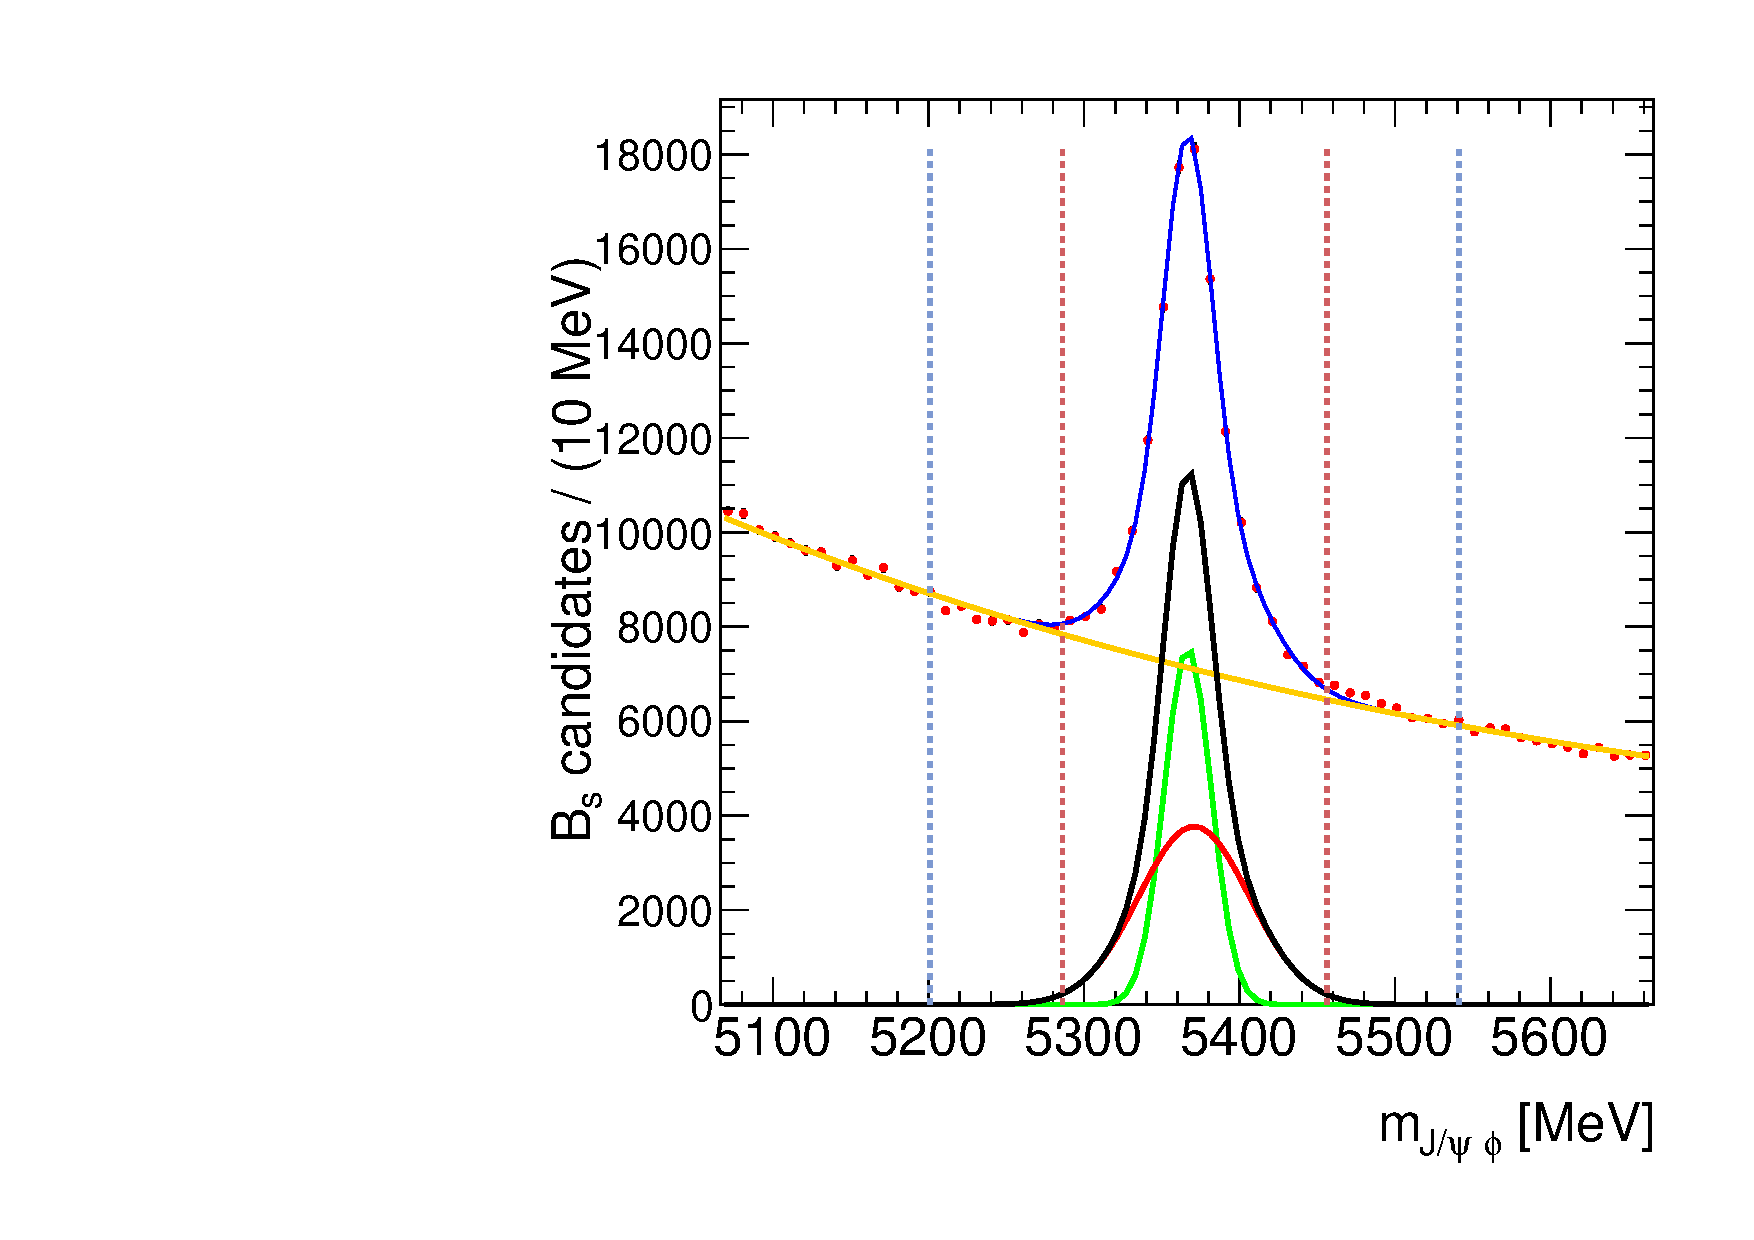
\includegraphics[width=0.47\textwidth]{figures/InternalNote_DataMCComparison/Bs/bsjpsiphibinnedfit.pdf}
\caption{Fit to the invariant mass distribution of \BsJpsiPhi\ events.}
\label{fig:jpsiphi}
\end{center}
\end{figure}

The data/MC comparisons of \pt{} and $\eta{}$ distributions for the \Bs\ are
shown in Figure~\ref{fig:xcheckcompBs}, while the distributions of few
discriminating variables are shown in Figure~\ref{fig:jpsiphivars}..
Finally the distribution of the continuum BDT variable is shown in
Figure~\ref{fig:jpsiphiBDT}.
The signal distributions in data are obtained by subtracting the
sideband shapes in each variable.

\yel[t.b.d.]{Additional studies of the} \BsJpsiPhi are presented in Section~\ref{sec:jpsiphi}.

\begin{figure}[!htb]
\begin{center}
\hspace*{-0.6cm}
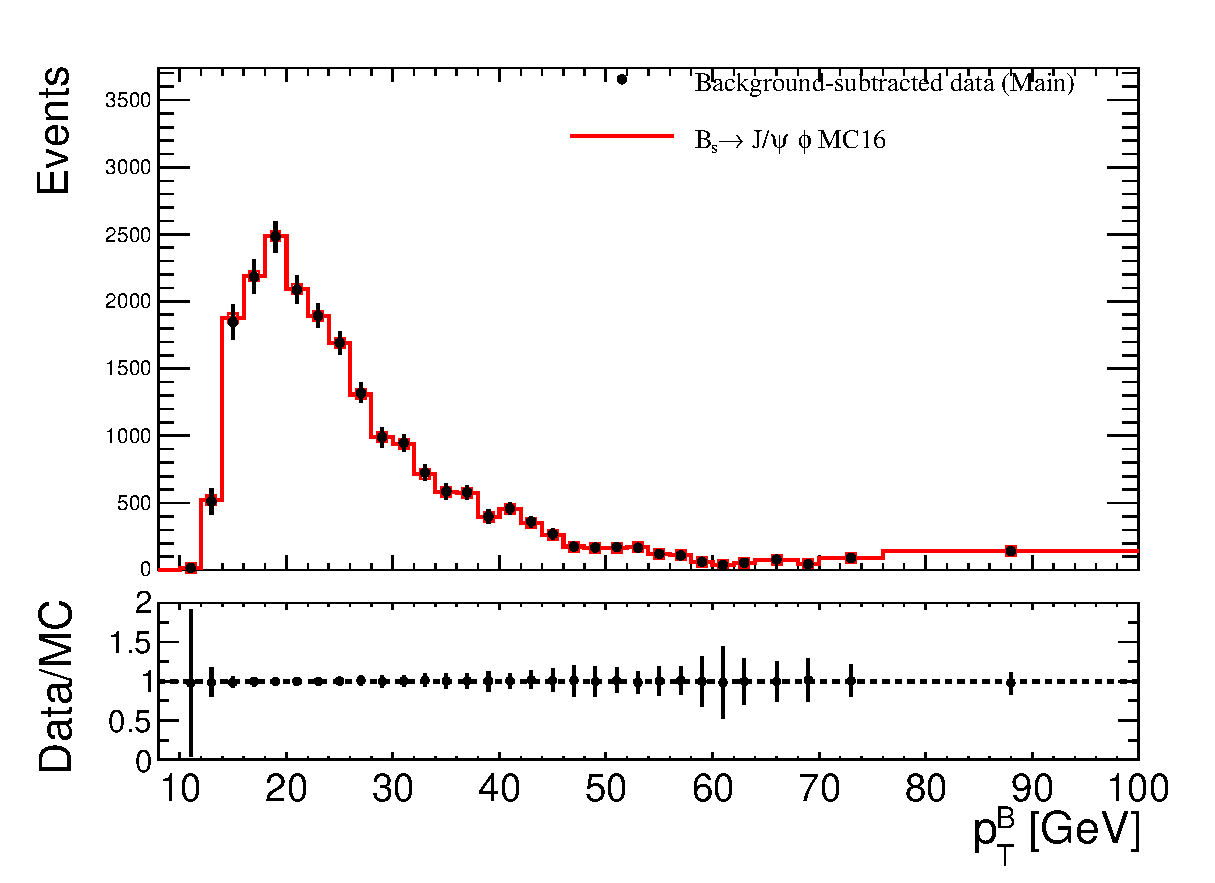
\includegraphics[width=0.52\textwidth]{figures/InternalNote_DataMCComparison/Bs/bsjpsiphi_pT.eps}
\hspace*{-0.6cm}
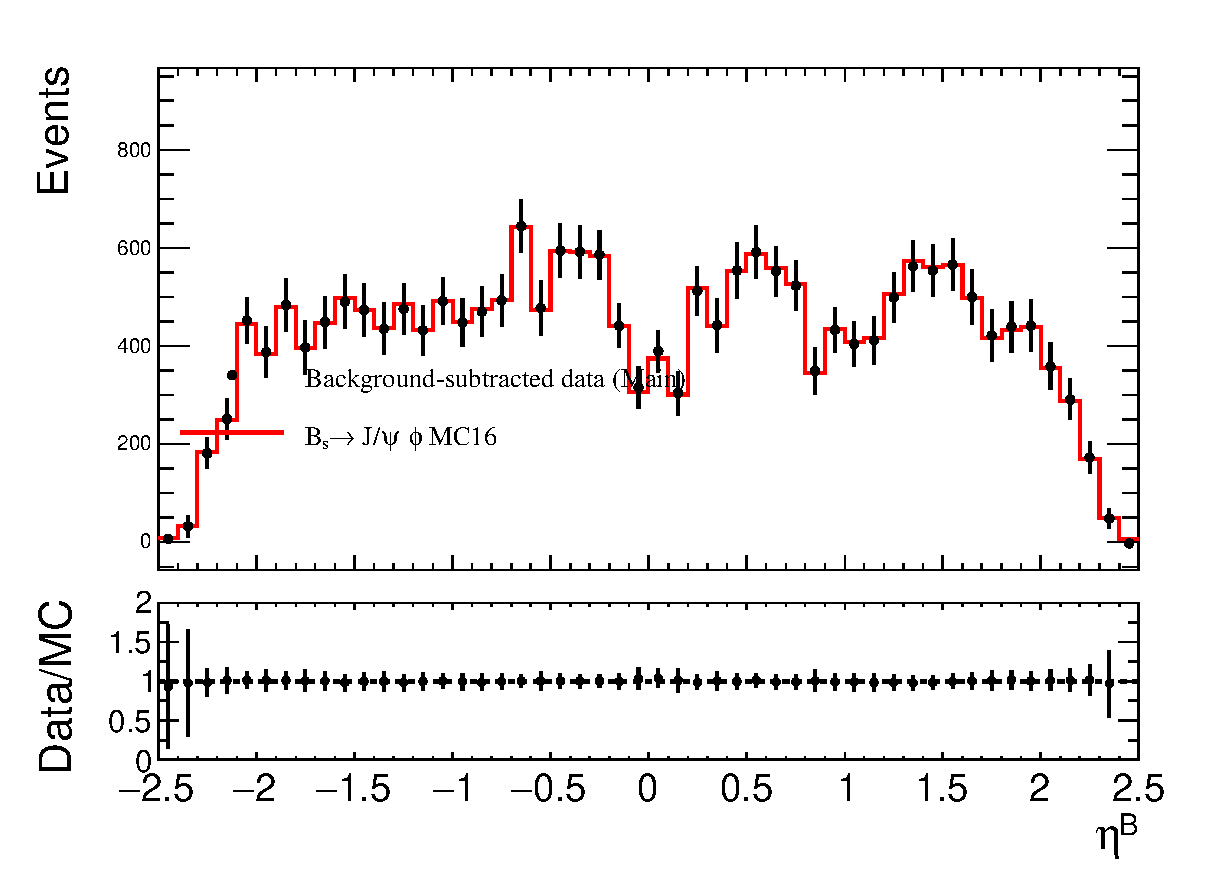
\includegraphics[width=0.52\textwidth]{figures/InternalNote_DataMCComparison/Bs/bsjpsiphi_eta.eps}
\caption{Cross-check on the \pt$^B$ and $\eta^B$ distributions of
the $J/\psi \phi$ candidates in data and signal MC.
The black dots correspond to the sideband subtracted data, while 
the red histograms correspond to reweighted MC 
normalised to the number of data events.}
\label{fig:xcheckcompBs}
\end{center}
\end{figure}
%
\begin{figure}[!htb]
\begin{center}
\hspace*{-0.5cm}
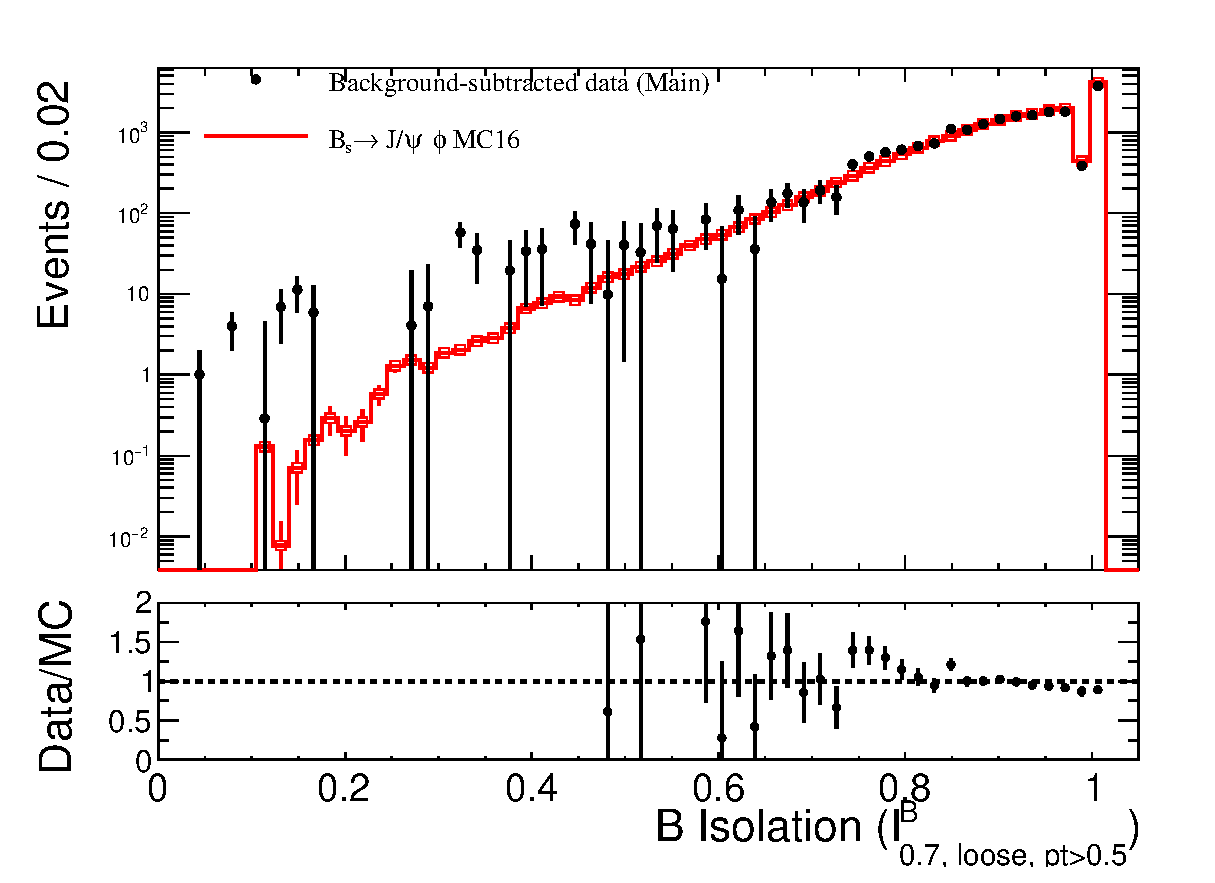
\includegraphics[width=0.48\textwidth]{figures/InternalNote_DataMCComparison/Bs/bsjpsiphi_iso.eps}
\hspace*{-0.5cm}
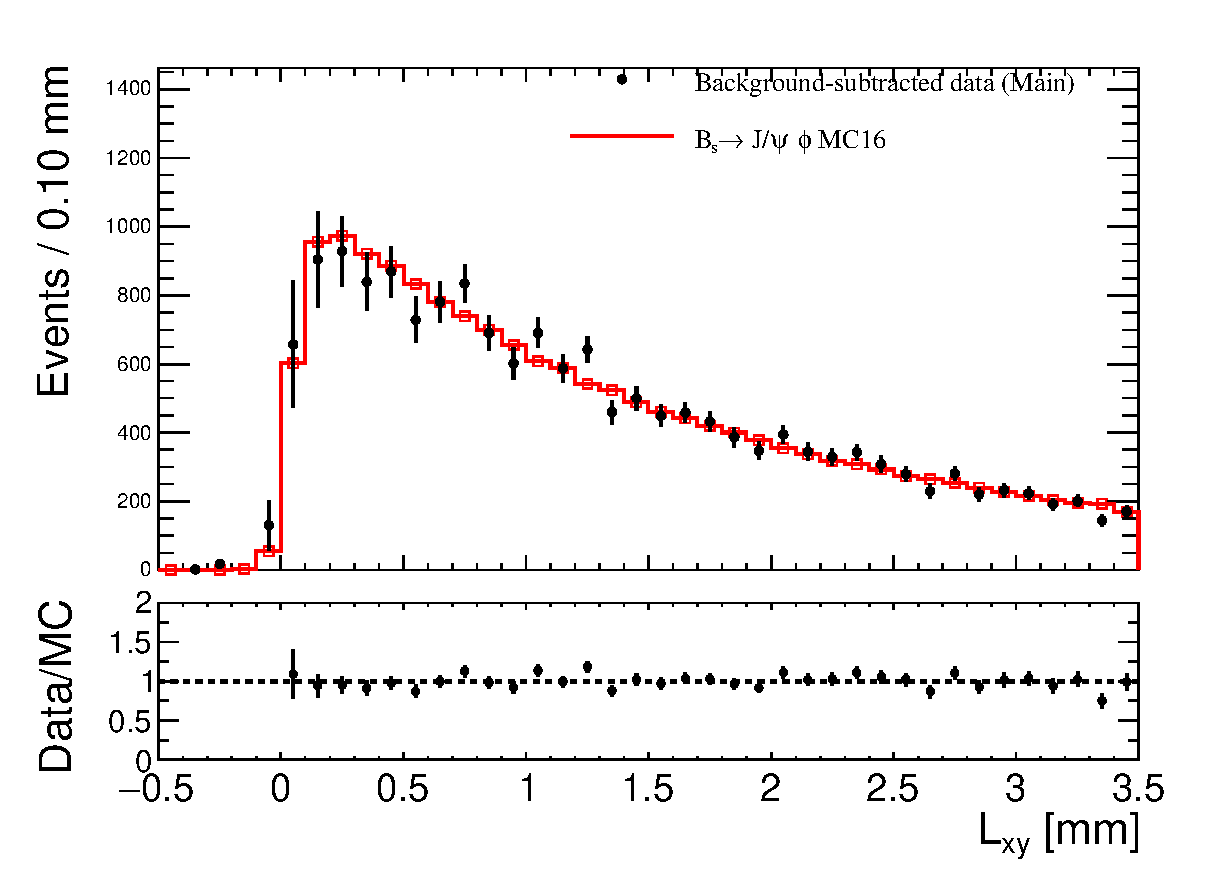
\includegraphics[width=0.48\textwidth]{figures/InternalNote_DataMCComparison/Bs/bsjpsiphi_Lxy.eps}\\
\hspace*{-0.5cm}
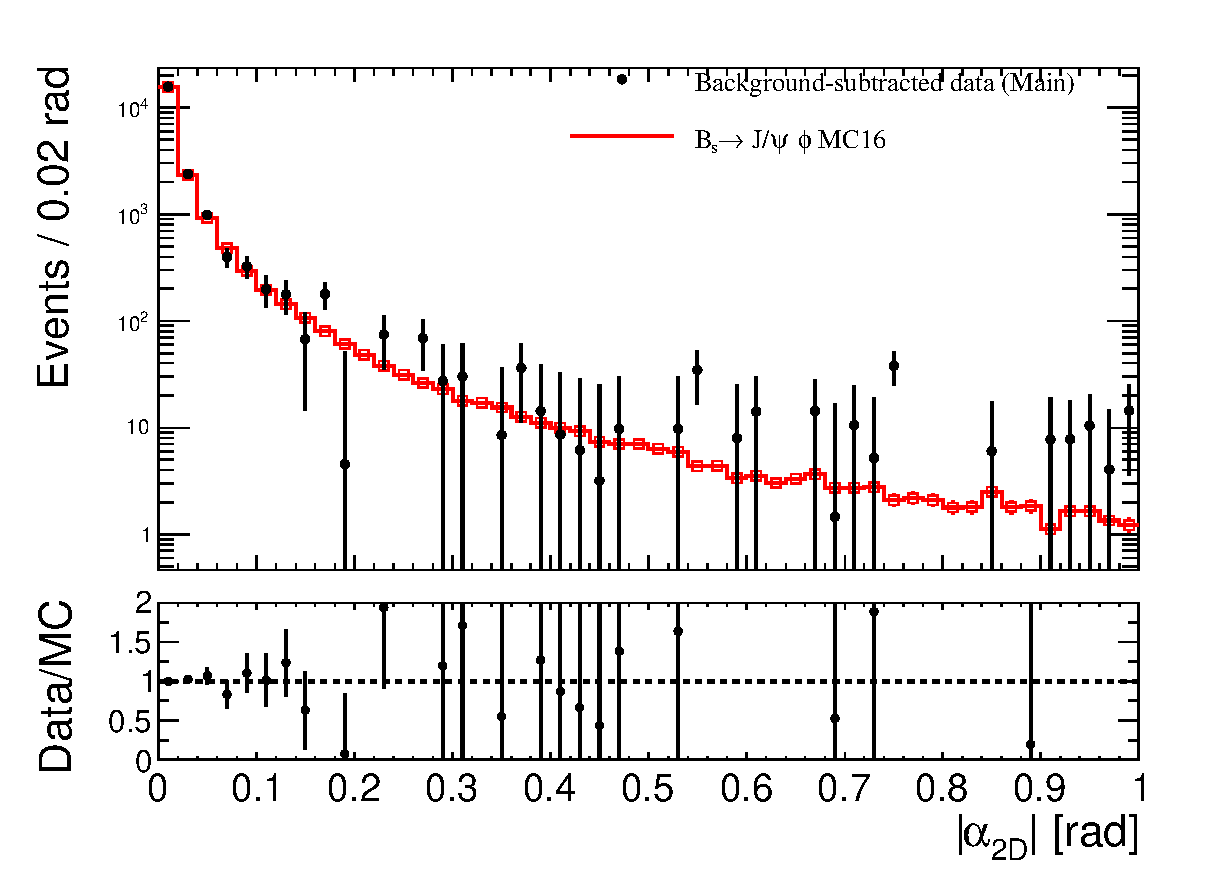
\includegraphics[width=0.48\textwidth]{figures/InternalNote_DataMCComparison/Bs/bsjpsiphi_a2D.eps}
\hspace*{-0.5cm}
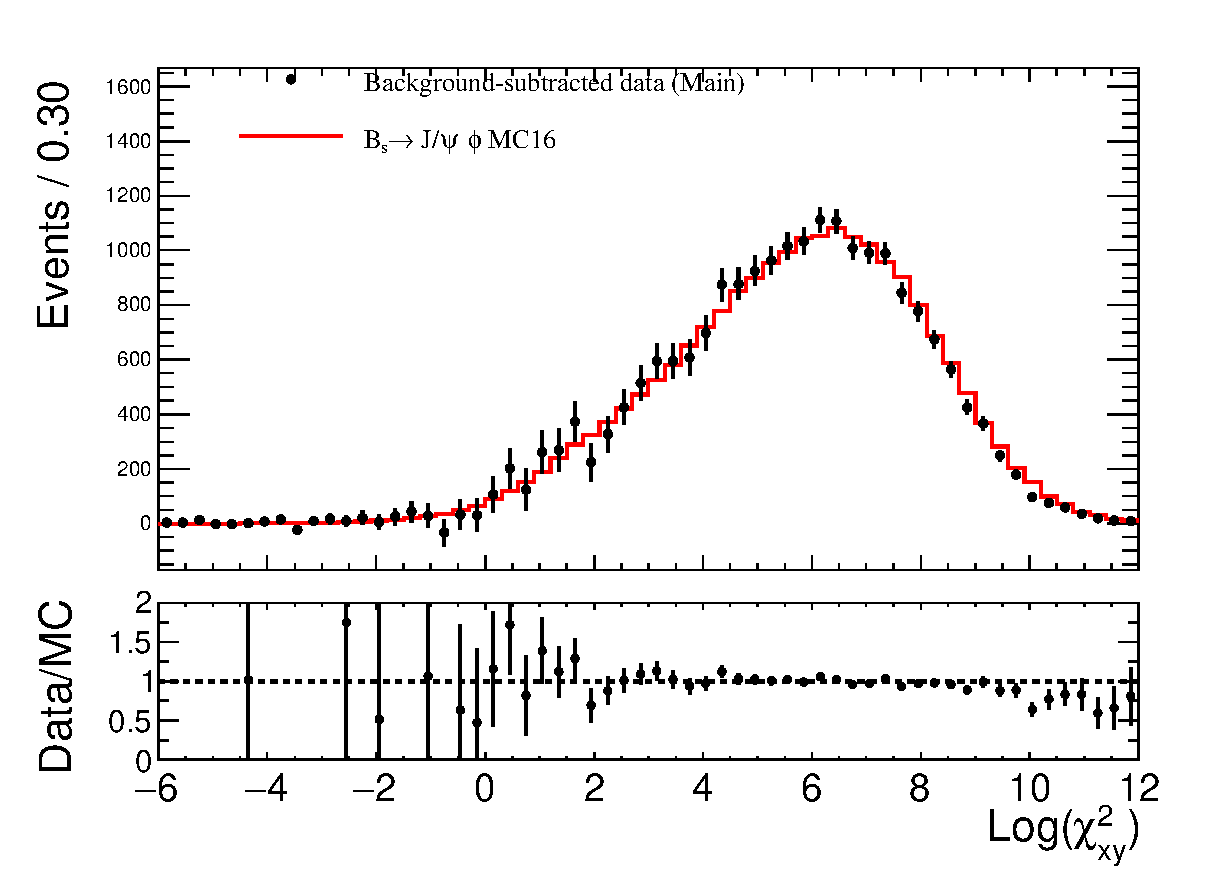
\includegraphics[width=0.48\textwidth]{figures/InternalNote_DataMCComparison/Bs/bsjpsiphi_chi2PVSV.eps}
\caption{{\it{From left to right, from top to bottom}}: 
Data and signal MC distributions of \BsJpsiPhi\ events for the $B$ isolation variable, 
the transverse decay length ($L_{xy}$), $|\alpha_{2D}|$ and 
$\chi^{2}_{xy}$ that represents the separation between production
(PV) and decay (SV) vertices.
The black dots correspond to the sideband subtracted data, while 
the red points correspond to reweighted MC normalised to the number
of data events.}
\label{fig:jpsiphivars}
\end{center}
\end{figure}
%
\begin{figure}[!b]
\begin{center}
\hspace*{-0.4cm}
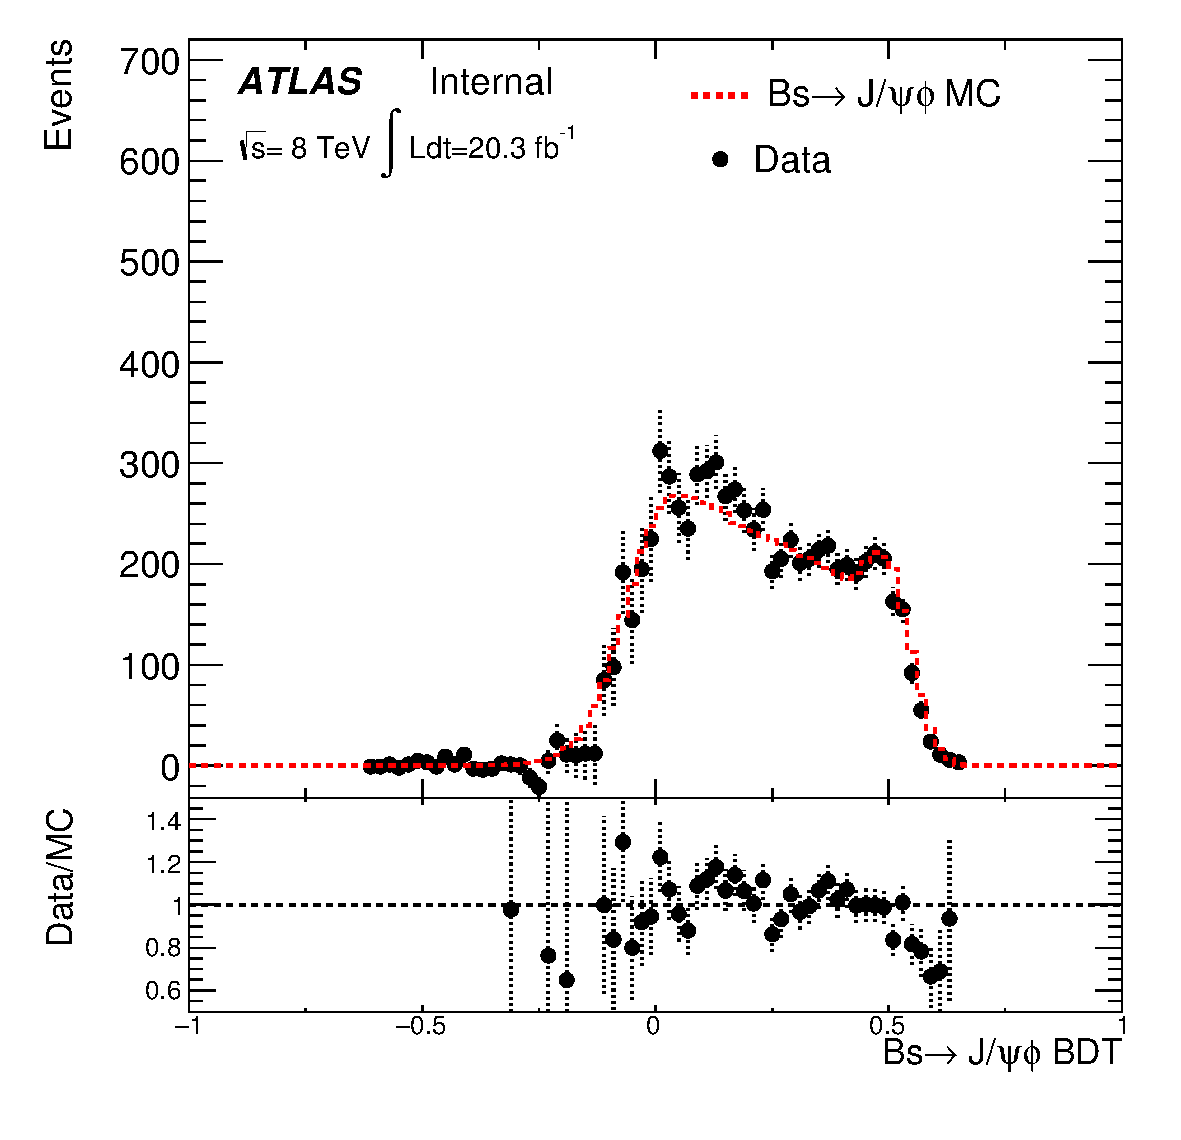
\includegraphics[width=0.47\textwidth]{figures/InternalNote_DataMCComparison/compRun1/Bs/BsJpsiphi_BDT12.pdf}
\hspace*{-0.4cm}
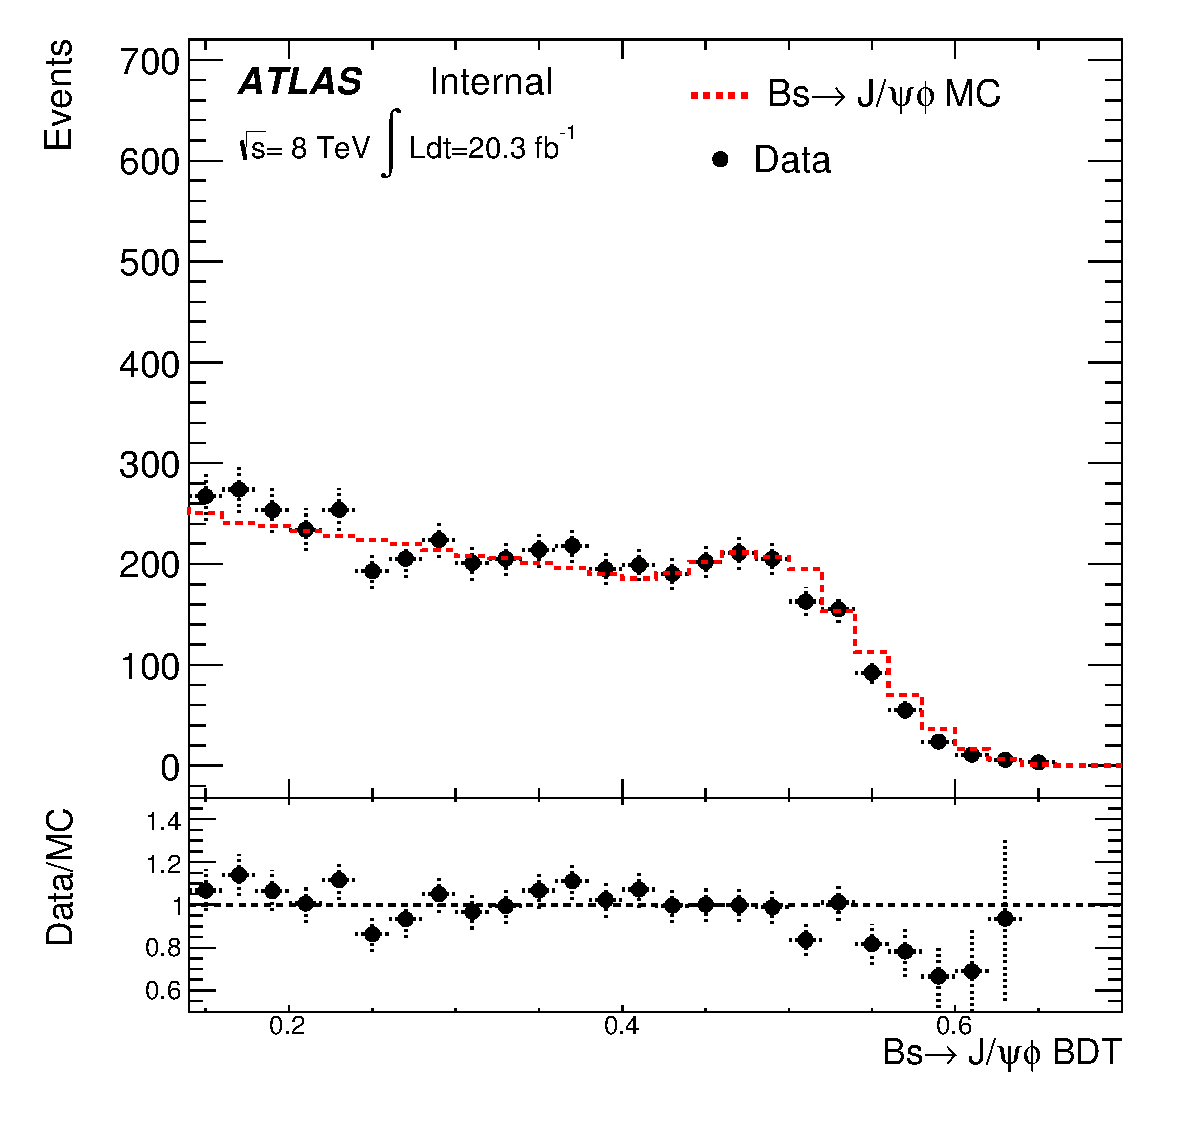
\includegraphics[width=0.47\textwidth]{figures/InternalNote_DataMCComparison/compRun1/Bs/BsJpsiphi_BDT12zoomed.pdf}
\caption{\textbf{Run 1 result, t.b.u.!}Data and signal MC distribution in \BsJpsiPhi\ events for the
continuum BDT variable.
The black dots correspond to the sideband subtracted data, while 
the red points correspond to reweighted MC normalised to the number
of data events. The left plot shows the same distribution zoomed
in the region of interest of the analysis.}
\label{fig:jpsiphiBDT}
\end{center}
\end{figure}
%
%BsJpsiphi_valid2_DR.pdf
 
\subsection{Yield stability during run}
\label{sec:stability}
The stability of the gain in the \Bs sidebands in the 2015 and 2016 data taking periods is shown in Figure~\ref{fig:gainstability}. The gain is calculated as the yield of events per period divided by the luminosity in that period. The gain appears to be stable during the run, within statistical uncertainties.
%The main variations correspond to the increase in trigger efficiency with the introduction of the L2StarB algorithm,
%occurring at 1.36~fb$^{-1}$ in the charged mode and at 6.19~fb$^{-1}$ in the neutral one.
\begin{figure}[!htb]
\begin{center}
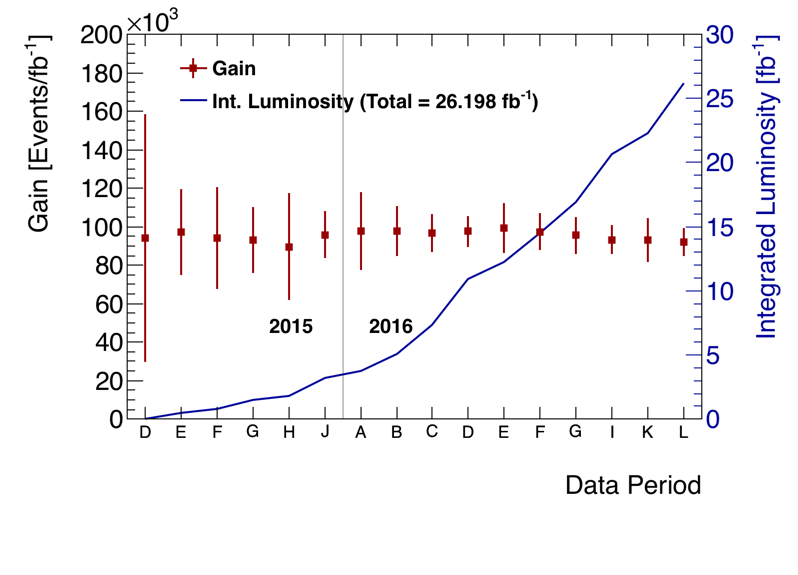
\includegraphics[width=0.7\textwidth]{figures/InternalNote_DataMCComparison/comp/GainPlot.png}
% \hspace*{-0.4cm}
% \includegraphics[width=0.47\textwidth]{figures/InternalNote_DataMCComparison/compRun1/Bplus-per-period.pdf}
% \hspace*{-0.4cm}
% \includegraphics[width=0.47\textwidth]{figures/InternalNote_DataMCComparison/compRun1/Bplus-BDTeff-per-period.pdf}\\
% \hspace*{-0.4cm}
% \includegraphics[width=0.47\textwidth]{figures/InternalNote_DataMCComparison/compRun1/Bs-per-period.pdf}
% \hspace*{-0.4cm}
% \includegraphics[width=0.47\textwidth]{figures/InternalNote_DataMCComparison/compRun1/Bs-BDTeff-per-period.pdf}
\caption{Stability of \Bs\ gain for 2015 and 2016 data taking periods. Also shown is the integrated luminosity for the analysis when the HLT\_mu4\_mu6\_bBmumu and HLT\_mu4\_mu6\_bBmumu\_Lxy0 triggers are applied to the 2015 and 2016 data respectively.}
\label{fig:gainstability}
\end{center}
\end{figure}


\clearpage

% B+ yield extraction
\graphicspath{ {figures/InternalNote_BPlusYield/} }

\section{BPlus Yield}
\label{sec:BPlusYield}

\subsection{Preselection}
Before carrying out the fit, a reasonably large $\bpjpsik$ signal has to be isolated
in the data. In order to do this we apply the following selection:

\begin{itemize}
    \item \textbf{Trigger: } We require our events to pass \verb|HLT_mu6_mu4_bJpsimumu|.
    \item \textbf{Requirements on B: } $M(B^+)\in [4930, 5630]\MeV$ and $\chi^2/NdoF < 6$ and $p_{T}(B^+)>8\GeV$.
    \item \textbf{Requirements on $J/\psi$: } $M(J/\psi)\in [2915, 3275]\MeV$ and $\chi^2/NdoF < 10$.
    \item \textbf{Kinematics on B: } $DR<1.5$ and $|a_{2D}|<1$ and $L_{xy}>0$.
    \item \textbf{BDT: } $BDT > 0.24$ We used the same xml file as in Run I, for now.
\end{itemize}

This selection is applied to 2015 data and the BDT was trained in 2012 data with the 
background as the combinatorial contribution to the $\bsmumu$ signal (see figure \ref{fig:reco_truth_assoc_comb}).
However this BDT will be updated eventually to use 2015 data. Figure \ref{fig:bplus_bdt_score} shows
the normalized distributions of the BDT score for both signal MC, data and the background.

\begin{figure}[ht]
    \centering
    \subfloat[]
    {
	\includegraphics[width=0.45\textwidth]{BDT_Wide.pdf}
    }
    \subfloat[]
    {
	\includegraphics[width=0.45\textwidth]{BDT_Narrow.pdf}
    }
    \caption{BDT score distribution for signal MC, background and data.}
    \label{fig:bplus_bdt_score}
\end{figure}

The background was extracted from the $\bbjpsix$ sample, after the signal component was filtered out.
The cutflow for the three samples can be seen in figure \ref{fig:bplus_fit_cutflow}.

\begin{figure}[ht]
    \centering
    \subfloat[Background]
    {
	\includegraphics[width=0.45\textwidth]{B_VTX_mass_background.pdf}
    }
    \subfloat[Signal]
    {
	\includegraphics[width=0.45\textwidth]{B_VTX_mass_signal.pdf}
    }

    \subfloat[Data]
    {
	\includegraphics[width=0.45\textwidth]{B_VTX_mass_data.pdf}
    }
    \caption{Cutflow associated to the simulated $\bsmumu$ and $\bpjpsik$ samples, and for the data.}
    \label{fig:bplus_fit_cutflow}
\end{figure}

In these figures \textit{No signal} implies removing the $\bpjpsik$ component
from the respective sample, this obviously only makes sense for the $\bbjpsix$ sample,
otherwise it has no effect. The corresponding efficiencies are in tables \ref{tbl:bplus_cutflow_eff_background},
\ref{tbl:bplus_cutflow_eff_signal} and \ref{tbl:bplus_cutflow_eff_data}. After applying 
this selection the background composition is as shown in table \ref{tbl:bplus_bckg_selection}.

\begin{table}[ht]
    \centering
    \begin{tabular}{| l | c | r |}
	\hline
	Cut   & Efficiency & Number of Events\\ 
	\hline
	No Signal & 0.91 & 1695814\\ 
	Trigger & 0.37 & 629375\\ 
	Cuts on B & 0.15 & 251257\\ 
	Cuts on $J/\psi$ & 0.15 & 249617\\ 
	Cuts on kinematic quantities & 0.13 & 215851\\ 
	BDT & 0.02 & 31101\\ 
	\hline
    \end{tabular}
    \caption{Cutflow efficiency for $\bbjpsix$ sample.}
    \label{tbl:bplus_cutflow_eff_background}
\end{table}

\begin{table}[ht]
    \centering
    \begin{tabular}{| l | c | r |}
	\hline
	Cut   & Efficiency & Number of Events\\ 
	\hline
	No Signal & 1.00 & 990211\\ 
	Trigger & 0.43 & 429273\\ 
	Cuts on B & 0.36 & 353872\\ 
	Cuts on $J/\psi$ & 0.35 & 351176\\ 
	Cuts on kinematic quantities & 0.34 & 335628\\ 
	BDT & 0.19 & 188707\\ 
	\hline
    \end{tabular}
    \caption{Cutflow efficiency for $\bpjpsik$ sample.}
    \label{tbl:bplus_cutflow_eff_signal}
\end{table}

\begin{table}[ht]
    \centering
    \begin{tabular}{| l | c | r |}
	\hline
	Cut   & Efficiency & Number of Events\\ 
	\hline
	No Signal & 1.00 & 23470163\\ 
	Trigger & 0.66 & 15553565\\ 
	Cuts on B & 0.33 & 7691019\\ 
	Cuts on $J/\psi$ & 0.32 & 7602035\\ 
	Cuts on kinematic quantities & 0.16 & 3860800\\ 
	BDT & 0.01 & 292550\\ 
	\hline
    \end{tabular}
    \caption{Cutflow efficiency for data.}
    \label{tbl:bplus_cutflow_eff_data}
\end{table}

\begin{table}[ht]
    \centering
    \begin{tabular}{| l | r |}
	\hline
	Frequency & Decay\\ 
	\hline
	11015 & B0[K*0[pi-:K+]J/psi[mu+:mu-]] \\ 
	7797 & unmatched \\ 
	3598 & B+[K*+[pi0[gamma:gamma]K+]J/psi[mu+:mu-]] \\ 
	1750 & B+[K+:chi\_1c[gamma:J/psi[mu+:mu-]]] \\ 
	1411 & B+[pi+:J/psi[mu+:mu-]] \\ 
	751 & B0[K*0[pi-:gamma:K+]J/psi[mu+:mu-]] \\ 
	471 & B0[pi-:K+:J/psi[mu+:mu-]] \\ 
	442 & B+[rho+[pi0[gamma:gamma]pi+]J/psi[mu+:mu-]] \\ 
	278 & B0[K*\_20[pi-:K+]J/psi[mu+:mu-]] \\ 
	252 & B+[K*+[pi+:K0[K\_S0]]J/psi[mu+:mu-]] \\ 
	250 & B+[K*+[pi+:K0[K\_L0]]J/psi[mu+:mu-]] \\ 
	239 & combinatorial \\ 
	214 & B+[pi0[gamma:gamma]K+:J/psi[mu+:mu-]] \\ 
	191 & B0[rho0[pi-:pi+]J/psi[mu+:mu-]] \\ 
	187 & B+[gamma:pi+:J/psi[mu+:mu-]] \\ 
	149 & B\_s0[pi-:pi+:J/psi[mu+:mu-]] \\ 
	135 & B\_s0[eta'[gamma:rho0[pi-:pi+]]J/psi[mu+:mu-]] \\ 
	118 & B+[gamma:K*+[pi0[gamma:gamma]K+]J/psi[mu+:mu-]] \\ 
	118 & B+[K+:chi\_0c[gamma:J/psi[mu+:mu-]]] \\ 
	102 & B+[K*\_2+[pi0[gamma:gamma]K+]J/psi[mu+:mu-]] \\ 
	89 & B*-[B-[K-:J/psi[mu+:mu-]]gamma] \\ 
	81 & missing particles \\ 
	79 & B+[gamma:K+:chi\_1c[gamma:J/psi[mu+:mu-]]] \\ 
	76 & B+[K*\_2+[pi+:K0[K\_L0]]J/psi[mu+:mu-]] \\ 
	76 & B+[K*\_2+[pi+:K0[K\_S0]]J/psi[mu+:mu-]] \\ 
	69 & B+[pi+:K0[K\_L0]J/psi[mu+:mu-]] \\ 
	52 & B+[pi+:K0[K\_S0]J/psi[mu+:mu-]] \\ 
	41 & B+[K*+[pi0[e+:e-:gamma]K+]J/psi[mu+:mu-]] \\ 
	39 & Xi\_b+[Xi-\_bar:J/psi[mu+:mu-]] \\ 
	\hline
    \end{tabular}
    \caption{Background composition of $\bbjpsix$ sample selection is applied.}
    \label{tbl:bplus_bckg_selection}
\end{table}

Additionally figure \ref{fig:decay_distribution} shows the distribution of the number of decays
versus the index of the decay, when the most common decays are put at the beginning, the plot
also shows the corresponding cumulative distribution.

There are 81 candidates classified as \textit{missing particle} for which the matching is not possible
given that there are no particles in the event record, that follow the requirements. 

\begin{figure}
    \centering
    \includegraphics[width=0.70\textwidth]{decay_frequency.pdf}
    \caption{Decay distribution and the corresponding cumulative distribution.}
    \label{fig:decay_distribution}
\end{figure}

\subsection{Procedure}
To extract the $B^+$ yield for the reference channel, we use a
unbinned maximum likelihood fit to the mass distribution.
The fit is performed simultaneously on data and the MC samples
from which the models are taken.
With respect to the 2011 analysis, the event-by-event error is
no longer used as it provides very limited or no separation.

\begin{figure}[!htb]
    \begin{center}
	\hspace{-0.5cm}
	\includegraphics[width=0.52\textwidth]{dataonlyN3.eps}
	\hspace{-0.5cm}
	\includegraphics[width=0.52\textwidth]{mcprdN3.eps}
	\caption{{\it Left}: $J/\psi K^{\pm}$ invariant mass distribution for all $B^{\pm}$
	    candidates in 2012 data.
	    {\it Right}: partially reconstructed $B$ decays contributing to the background
	as described by Monte Carlo.}
	\label{fig:bplusinvmass}
    \end{center}
\end{figure}

In the $B^\pm$ invariant mass distribution (shown in Figure~\ref{fig:bplusinvmass},
left plot) the $B^\pm$ signal is quite evident, but with visible contributions
from at least three background categories. On the left of the $B^\pm$ peak
we find the partially reconstructed $B$ decays
(PRD, e.g. $B^{+/0} \to K^{*+/0} J/\psi$, $B^{+} \to K^{+} \chi_{c1,2}$) 
where one or more of the final state particles are missed in the reconstruction.
On the right side, it is expected a contribution from the reflection of the
Cabibbo-suppressed $B^\pm\to J/\psi\pi^\pm$ decay with the assignment of the
kaon mass to the final state pion.
Finally there is the combinatorial background, which MC studies suggest to be composed,
after our selection cuts, mostly of $b\bar{b}\to \jpsi X$ that spans on the whole mass
range, and consists of random combination of \jpsi\ (produced promptly in $pp$ collisions
or in feed-down from B-decays) with a track.

For the extraction of the $B^+$ yield, we define the following event categories:
\begin{itemize}
    \setlength{\itemsep}{0pt}%
	\setlength{\parskip}{0pt}%
    \item \NJpsiK{}: number of \BpmKpmJpsi{} events (signal events for this fit);
    \item \NJpsipi{}: number of \BpPipJpsi{} events;
    \item \Npr{}: number of partially reconstructed events (PRD);
    \item \Nc{}: number of combinatorial events.
\end{itemize}

Table~\ref{tab:fit_candidates} shows the \BpmKpmJpsi{} candidates, in the mass region
$4930-5630\ \mathrm{MeV}$, passing the complete selection (including the final
continuum BDT cut). 

\begin{table}[!htb]
    \begin{center}
	%input{appendix/bplusfit_table_data.tex}
	\label{tab:fit_candidates}
    \end{center}
\end{table}

The fit is based on a unbinned extended maximum likelihood fit to data
with simultaneous inclusion of three MC samples to guide the modeling of
several fit components.
The MC samples are introduced to model accurately the shapes of the \BpmKpmJpsi{} 
events as well as the most critical background components: the PRD and the
$J/\psi\pi^\pm$ decays.
By fitting the above mentioned MC samples simultaneously, we constrain the
fit parameters of the corresponding fit components to their MC values.
This results in an \textit{MC assisted} determination of the background shapes,
while automatically accounting for the statistical uncertainties of the MC.
Two free parameters, one for the mass scale and the other for the mass resolution
are extracted from data to accommodate for the possible data-MC difference
in the shapes for \BpmKpmJpsi{}, PRD and $J/\psi\pi^\pm$ decays.

The probability density functions (PDF's) used in this fit are described
below. The parameters of each function are tied among the data and MC samples,
so that effectively the parameter values that are determined by the fit
on the MC components are propagated to functions used to fit the data
components.

The three MC samples included in the simultaneous fit are:
\begin{itemize}
    \setlength{\itemsep}{0pt}%
	\setlength{\parskip}{0pt}%
    \item \BpmKpmJpsi{} MC events: $B^+\to J/\psi K^+$ ($J/\psi\to\mu^+\mu^-$)
	exclusively generated. These events include also radiative decays where
	the $B^\pm$ radiates a $\gamma$. The two cases are modeled separately in
	the fit but they are both included in the signal definition.
    \item $B^\pm\to J/\psi\pi^\pm$ MC: used to describe this reflection when the
	$K$ mass is mis-assigned to the final state pion.
    \item $bb\to J/\psi X$ MC sample: PRD events are characterized by this sample.
	Where we can distinguish the true origin of each reconstructed
	$B^\pm$ candidate. In order to model the PRD contribution to the mass fit,
	we identify three classes of decays contributing with slightly different mass shapes.
	The three classes are as follows:
	\begin{itemize}
	    \item PRD1: these events produce a step shape at 5150 MeV:
		these are mainly
		$B^0\rightarrow J/\psi  K^{*0}$,
		$B^+\rightarrow J/\psi  K^{*+}$,
		$B^0\rightarrow J/\psi  \rho^{0}$,
		$B^+\rightarrow J/\psi  \rho^{+}$,
		$B^0\rightarrow J/\psi  K^+\pi^-$, and
		$B^+\rightarrow J/\psi  K^+\pi^{0}$.
	    \item PRD2: these events produce a bump at 5050 MeV.
		These events are mainly 
		$B^+\rightarrow\chi_{c1}K^+$.
		%and $B^+\rightarrow \chi_{c2}K^+$.
	    \item PRD3: this component includes everything else
		from the $J/\psi X$ sample and has a smoother shape
		in the mass distribution.
	\end{itemize}
\end{itemize}

The PDF's used are the following:
\begin{itemize}
    \setlength{\itemsep}{0pt}%
	\setlength{\parskip}{0pt}%
    \item \BpmKpmJpsi{} signal:
	Johnson $S_U$~\cite{Johnson}, this PDF contains the core of the signal events and
	it is parameterized as follows:
	\begin{equation}
	    \mathrm{Johnson}~S_U =
	    \frac{1}{\sqrt{1+t^2}}\left[t+\sqrt{1+t^2}\right]^{-\gamma-\frac{1}{2}\delta\ln{(t+\sqrt{1+t^2})}} \text{, where } t = \frac{m-\xi}{\lambda}
	\end{equation}
	where $\xi = s_\mu + \xi^{MC}$ in which $s_\mu$ parameterizes the
	possible mass scale shift between data and MC. The same $s_\mu$
	scale shift is applied to the Gaussian mean: $s_\mu+\mu^{MC}$ where
	$\mu^{MC}$ is the mean of the Gaussian shape in the \BpmKpmJpsi{} MC sample.
	Parameters $\lambda$, $\xi$, $\delta$ and $\gamma$ determine the shape
	of the distribution Johnson $S_U$ distribution. The parameters $\xi$
	and $\lambda$ control the position and width of the distribution,
	respectively. The sign of $\gamma$ determines the position of
	the tail (left or right to the peak).

	A data-MC discrepancy is allowed also in the resolution parameters:
	the Johnson $S_U$ distribution is convoluted with a Gaussian resolution function
	with zero mean and $s_\sigma$ width where the latter parameter describes 
	the resolution difference between data and MC.
	The same effect is taken into account in the Gaussian distribution
	whose width is thus obtained by summing in quadrature the MC width
	$\sigma^{MC}$ and the resolution smearing factor $s_\sigma$.

	The model of the shape is taken from \BpmKpmJpsi{} MC events
	and its parameters are left floating in the fit to be determined from
	the \BpmKpmJpsi{} MC sample in the simultaneous fit.
	The normalization and the $2$ scaling factors allow the distribution to
	adjust to the data peak.
	Details on the specific implementation of these parameterizations
	are found in Appendix~\ref{app:sec:bplusfitsigdescription}.

    \item radiative contribution to \BpmKpmJpsi{} decays: when the $B$ radiates a $\gamma$,
	the mass shape results skewed on the left so we need to consider
	this component separately. A single Johnson $S_U$ is used. 

	The shape parameters are determined from the radiative decays selected
	in the $J/\psi K^\pm$ MC sample.
	The normalization and the $2$ scaling factors allow the distribution to
	adjust to the data peak.
	Details on the specific implementation of these parameterizations
	are found in Appendix~\ref{app:sec:bplusfitsigdescription}.

	The relative abundances of the two signal components (non-radiative
	and radiative) are parametrized using relative fractions so that
	the total number of \BpmKpmJpsi{} events is extracted from the fit
	together with the three fractions.

    \item $J/\psi\pi^\pm$ final states:
	similarly to the \BpmKpmJpsi{} component, a Johnson $S_U$. 
	Also in this case the shape parameters are determined
	from the $J/\psi\pi^\pm$ MC sample in the simultaneous fit.

	The $2$ overall scaling factors on the mass scale and resolution
	are also applied to these parameterizations: in the fit they are
	driven by the effect on the \BpmKpmJpsi{} component.

    \item PRD component:
	\begin{itemize}
	    \setlength{\itemsep}{0pt}%
		\setlength{\parskip}{0pt}%
	    \item PRD1 with 5150-step shape.
		We parameterize these events with a Fermi-Dirac (FD) plus an Exponential
		The FD distribution is parametrize as follows:
		\[
		    \mathrm{M_{FD}}(m|\mu_{FD}, \alpha_{FD})=\frac{1}{1+e^{\frac{m - \mu_{FD}}{\alpha_{FD}}}}
		\]
		where $\alpha_{FD}$ accounts for the slope, while $\mu_{FD}$ accounts for
		the mass scale at which the step-like effect occurs.
		The shape parameters are taken from the PRD1 events in the
		$(bb\to\mu^-\mu^+X)_{\mathrm{pr}}$ MC sample in the simultaneous fit.
		In the parameterization used for data the FD mass scale parameter $\mu_{FD}$
		is redefined as $\mu^{MC}_{FD} + s_\mu$ where $s_\mu$ is the scale factor
		already defined above and it is common to the \BpmKpmJpsi{} and $J/\psi\pi^\pm$ events.
		The PDF is then convoluted with the Gaussian resolution function
		with the $s_\sigma$ width already defined above and common to the \BpmKpmJpsi{}
		and $J/\psi\pi^\pm$ events.

	    \item PRD2 with 5000-bump shape.
		We parameterize these events with a FD plus an Exponential
		Again the $2$ overall scaling factors on
		the mass scale and resolution are applied to these parameterizations.
		The shape parameters are taken from the PRD2 events in the
		$(bb\to\mu^-\mu^+X)_{\mathrm{pr}}$ MC sample in the simultaneous fit.

	    \item PRD3 with a falling shape.
		We parameterize these events with an Exponential plus a constant term.
		Again the $2$ overall scaling factors on
		the mass scale and resolution are applied to these parameterizations.
		The shape parameters are taken from the PRD3 events in the
		$(bb\to\mu^-\mu^+X)_{\mathrm{pr}}$ MC sample in the simultaneous fit.

	\end{itemize}
	Details on the specific implementation of these parameterizations
	are found in Appendix~\ref{app:sec:bplusfitPRDdescription}.
	The relative abundances of the PRD three components are taken from 
	the MC predictions, while the PDG values of these are used as a
	systematic check.
	The total number of PRD events is extracted from the data fit.

    \item combinatorial background:
	exponential function
	\[
	    \mathrm{M_{c}}(m|a)=e^{a m}
	\]
	with the shape parameter that is left floating in the fit
	to be extracted from data.
\end{itemize}

Figures~\ref{fig:bplusfitN12} and~\ref{fig:bplusfitN32011} show the results of the fits: 
the projection on the \Bp\ mass are shown for data.
Appendix~\ref{app:bplusfits} contains the complete fit results including the 
projections on the mass for the MC samples.
As an example, we show in Figure~\ref{fig:bplusfitN3all} all the simultaneous fit results. 
Table~\ref{tab:bplusfit3pars} shows the parameters from the fit, 
again as an example. In Appendix~\ref{app:bplusfits} similar
tables are shown.

\clearpage
\begin{figure}[!htb]
    \begin{center}
	\includegraphics[width=0.52\textwidth]{datafitN2.eps}
	\caption{Fit projection on 
	    The red line represents the \BpmKpmJpsi{} signal (including both radiative
	    and non-radiative components), while the magenta line represents the
	    $J/\psi\pi$ peaking component. The blue line shows all the three partially
	    reconstructed contributions and the green line represents the
	    combinatorial background. The total of all functions is presented
	with the black line.}
	\label{fig:bplusfitN12}
    \end{center}
\end{figure}

\begin{figure}[!htb]
    \begin{center}
	\hspace{-0.5cm}
	\includegraphics[width=0.52\textwidth]{datafitN3.eps}
	\hspace{-0.5cm}
	\includegraphics[width=0.52\textwidth]{datafitN2011.eps}
	\caption{Fit projection on data (left) and for the 2011 data (right).
	    The red line represents the \BpmKpmJpsi{} signal (including both radiative
	    and non-radiative components), while the magenta line represents the
	    $J/\psi\pi$ peaking component. The blue line shows all the three partially
	    reconstructed contributions and the green line represents the
	    combinatorial background. The total of all functions is presented
	with the black line.}
	\label{fig:bplusfitN32011}
    \end{center}
\end{figure}

\begin{figure}[!htb]
    \begin{center}
	\hspace{-0.5cm}
	\includegraphics[width=0.40\textwidth]{mcfitsigN3.eps}
	\hspace{-0.5cm}
	\includegraphics[width=0.40\textwidth]{mcfitradsigN3.eps}
	\hspace{-0.5cm}
	\includegraphics[width=0.40\textwidth]{mcfitjpsipiN3.eps}
	\hspace{-0.5cm}
	\includegraphics[width=0.40\textwidth]{mcfitprd1N3.eps}
	\hspace{-0.5cm}
	\includegraphics[width=0.40\textwidth]{mcfitprd2N3.eps}
	\hspace{-0.5cm}
	\includegraphics[width=0.40\textwidth]{mcfitprd3N3.eps}
	\caption{Fit projections on the MC samples simultaneous fitted with the data.
	    From left to right, from top to bottom: non-radiative \BpmKpmJpsi{} signal, 
	    radiative \BpmKpmJpsi{} signal, peaking background $J/\psi \pi$, PRD1, PRD2
	    and PRD3.
	    The red line is used for the \BpmKpmJpsi{} signal (including both radiative
	    and non-radiative components), while the magenta line is for the
	    $J/\psi\pi$ peaking component. The blue lines refer to all the three
	    partially reconstructed contributions.
	    In each plot, the black non-continuous lines show the single functions
	of the total PDF used to model the given component.}
	\label{fig:bplusfitN3all}
    \end{center}
\end{figure}

\clearpage
\begin{table}[!htb]
    \begin{center}
	%input{appendix/bplusfit_table_fitN3.tex}
	\label{tab:bplusfit3pars}.
    \end{center}
\end{table}

\subsection{Systematic Uncertainties in the Extraction of the $B^\pm$ Yields}
\label{sec:bplusyst}

Some of the systematic effects are taken care of automatically in the fit:
the MC effect of limited statistics, for example, is included in the statistical
fit error from the simultaneous fit. In addition the data-MC discrepancy in the
mass scale and resolution is included in the fit using the aforementioned scaling
factors.

Systematic effects on the reference channel yield are coming mainly from the parametrization
of the mass distributions and the data-MC discrepancies. The approximation of mass shapes in the
simultaneous fit by PDFs is a source of systematic uncertainty on the fit result which
we evaluate by repeating the fit varying the fit models. The difference between the modified
and default fit results is then taken as the systematic uncertainty.
The systematic uncertainties can be found in Table~\ref{tab:bplusyst} as
an example. 

The list of systematic checks is the following:
\begin{itemize}
    \setlength{\itemsep}{0pt}%
	\setlength{\parskip}{0pt}%
    \item data-MC discrepancies in $B$ kinematics: discrepancies on the $B$ meson kinematics
	between data and MC introduce a source of uncertainty. GLC- and DDW-weighted $J/\psi K^+$
	and $J/\psi \pi^+$ MC samples account for biases introduced by generator level
	preselection cuts and discrepancies in 2D ($p_{T}$,$\eta$) spectrum of the $B^{\pm}$ with
	respect to data. These reweighted samples are used as alternative MC samples in the simultaneous
	fit.

    \item Alternative model for the PRD3 component: in the PRD3 mass distribution we observe a
	structure not modeled by the Exponential PDF used. We account for this structure by
	adding a Gaussian to the default model.

    \item Combinatorial background model: the combinatorial background smoothly crosses our fit
	window and it is modeled with an exponential function in the default fit. This shape is not
	MC driven. We evaluate the systematic uncertainty coming from the unknown combinatorial
	background model by changing the model to a linear function.

    \item \BpmKpmJpsi{} signal peak charge asymmetry: the MC sample used in the default fit
	is from $B^+ \to J/\psi K^+$ events only. In order to account for shape variations relative to
	$B^- \to J/\psi K^-$, we repeat the fit using the latter.

    \item Alternative models for PRD1 and PRD2 components: systematics from the choice of PRD1
	and PRD2 models are assessed by replacing the principal (default) FD function with
	complementary error function ($\text{Erfc}(m) = \int_m^\infty \mathrm{e}^{-t^2}\,\mathrm{d}t $)
	in each of the two models.

    \item data-MC PRD composition discrepancies: the PRD MC sample has a relative decay modes
	abundances different than what would be expected according to current PDG measurements.
	Different abundances imply different mass shapes: we account for this data-MC shape
	discrepancy by introducing per-event weights derived from the Pythia and PDG differences.
	The weights correct for the MC shapes as well as for the relative abundances of the three
	PRD components. Two additional free parameters take care of the relative PRD fractions:
	these parameters have unit central values and are allowed to vary (via an external Gaussian
	constraint) within the PDG uncertainties on the BRs.

    \item including radiative tails into 2011 fit: When including radiative tails into 2011 fit
	we need to account for MC11-data11 discrepancies and 2011/2012 kinematic differences.
	To address the first issue, we use as alternate fitting sample 2011 MC weighted by the
	appropriate DDW obtained on 2011 data.
	To account for the MC11/MC12 kinematic differences we take the non-radiative $B^+$ candidates
	in the MC12 and the MC11 \BpmKpmJpsi{} signal, reweight both with the appropriate DDW(\&GLC) and obtain
	2011/2012 weights which we can use to reweight our 2012 MC radiative events to 2011 data
	conditions. These weights are also used in assessing the systematic effects from data-MC
	discrepancies in $B$ kinematics (first bullet above) for the 2011 fit.
	In addition, we perform two systematic fits changing the rad/non-rad fractions
	by $50\%$ and we take the largest variation on the result as systematic
	uncertainty.

\end{itemize}

The relative difference on the $B^+$ yields are given in table~\ref{tab:bplusystN3}. 

The main systematic uncertainties on the $B^+$ yield come from the
MC reweighting, the PRD reweighting and the combinatorial background
parametrization. The overall systematic uncertainties result to be
between $0.8-0.9\%$, depending on the data categories, as it is summarized
in Table~\ref{tab:bplusyst}.

\begin{table}[!htb]
    \begin{center}
	%input{appendix/bplusfit_table_systN3.tex}
	\label{tab:bplusystN3}
    \end{center}
\end{table}

\begin{table}[!htb]
    \begin{center}
	%input{appendix/bplusfit_table_syst.tex}
	\label{tab:bplusyst}
    \end{center}
\end{table}

\subsection{$B^{\pm} \rightarrow J\psi K^{\pm}$ yield results}

We measure the $B^{\pm} \rightarrow J\psi K^{\pm}$ reference channel yield with full
systematic uncertainty evaluation in the four measurement categories as shown in
Table~\ref{tab:bplusyieldresults}.

\begin{table}[!htb]
    \begin{center}
	%input{appendix/bplusfit_table_yieldresults.tex}
	\label{tab:bplusyieldresults}.
    \end{center}
\end{table}

\subsection{$J/\psi \pi^{\pm} / J/\psi K^{\pm}$ ratio measurement}
\label{sec:bpluspikratio}

From the fit described above, we extract both the yields for
$B^{\pm} \to J/\psi K^{\pm}$ and $B^{\pm} \to J/\psi \pi^{\pm}$ and
the systematic checks whose results are in Table~\ref{tab:bplusyst}
record the variation on both yields.
\begin{equation}
    \mathrm{R_{\pi/K}} = 
    \frac{N_{J/\psi \pi^{\pm}}\times I^{J/\psi\pi}_{ext}}{N_{J/\psi K^{\pm}}} 
\end{equation}
where the $J/\psi \pi^{\pm}$ yield is corrected by the factor $I^{J/\psi\pi}_{ext}$
explained below. Then we define the ratio:
\begin{equation}
    \rho_{\pi/K} = \frac{\mathcal{BR}(B^{\pm} \to J/\psi \pi^{\pm} )}
    {\mathcal{BR}(B^{\pm} \to J/\psi K^{\pm}) } 
    = \frac{N_{J/\psi \pi^{\pm}}\times I^{J/\psi\pi}_{ext} }{N_{J/\psi K^{\pm}}}\times
    \frac{\epsilon_{J/\psi K^{\pm} }}{\epsilon_{J/\psi \pi^{\pm}}}
    =\mathrm{R_{\pi/K}} \times 
    \left[\frac{\epsilon_{K^{+}}}{\epsilon_{\pi^{+}}} \times 
    \frac{1+\frac{{\epsilon_{K^{-}}}}{\epsilon_{K^{+}}}}{1+\frac{\epsilon_{\pi^{-}}}{\epsilon_{\pi^{+}}} }\right]
\end{equation}
where $N_{X}$ is the yield for channel $X$ ($J/\psi \pi^{\pm}$,
$J/\psi K^{\pm}$), and $\epsilon_{X}$ is the efficiency-times-acceptance
product for channel $X$.
In the last equality we have used the asymptotic relation
$\epsilon_h^\pm = \frac{\epsilon_h^+ + \epsilon_h^-}{2}$, and
$\frac{\epsilon_{K^{-}}}{\epsilon_{K^{+}}}$ and
$\frac{\epsilon_{\pi^{-}}}{\epsilon_{\pi^{+}}}$ are the kaon and pion
charge asymmetries, respectively.

The fit for the reference channel of Section~\ref{sec:bplus} extracts both
yields $J/\psi K^{\pm}$ and $J/\psi \pi^{\pm}$ from the fit mass window
$[4930.,5630.]$~MeV/$c^2$. While the $J/\psi K^{\pm}$ component is accommodated
entirely within our mass fit window, the $J/\psi \pi^{\pm}$ component extends
by a small fraction outside the right boundary. A fraction $I^{J/\psi \pi}_{ext.}$  of $J/\psi \pi^{\pm}$ candidates counted in the extended region $[3500.,7000.]$ MeV/$c^2$ with respect to the candidates counted in the default fit mass window is introduced as a correction for this small $J/\psi \pi^{\pm}$ tail. The result of such integration
$I^{J/\psi \pi}_{ext.}$ together with the corrected yield are summarized in
Table~\ref{tab:correctedjpsipi}. 

\begin{table}[!htb]
    \begin{center}
	%input{appendix/piKratio_table_jpsipi.tex}
	\label{tab:correctedjpsipi}
    \end{center}
\end{table}

Regarding the $\frac{\epsilon_{ K^{\pm} }}{\epsilon_{\pi^{\pm}}}$ ratio, 
three are the factors contributing:
the kaon and pion charge asymmetries ($\frac{\epsilon_{K^{-}}}{\epsilon_{K^{+}}}$,
$\frac{\epsilon_{\pi^{-}}}{\epsilon_{\pi^{+}}}$) and the relative $K^{+}/\pi^{+}$
efficiency  $\frac{\epsilon_{K^{+}}}{\epsilon_{\pi^{+}}}$. For the pion charge
asymmetry we assume the central value to be $\frac{\epsilon_{\pi^{-}}}{\epsilon_{\pi^{+}}} = 1$
and we assign an uncertainty to it as discussed below. We evaluate the remaining
two factors using Monte Carlo and estimate systematic uncertainties as described
below.

The four measurements of $\rho_{\pi/K}$ in the separate data categories are then
combined to minimize the measurement uncertainty.

Most systematic effects (luminosity, trigger, reconstruction efficiencies)
cancel in the measurement of this ratio due to the almost identical
topology and kinematics of the two decay channels. Residual systematic
uncertainties on the ratio of branching fractions come from uncertainties
on the parametrization of the fit PDFs, data-MC discrepancies, the
$K^{-}/K^{+}$ and $\pi^{-}/\pi^{+}$ charge asymmetries, and the
$K^{+}/\pi^{+}$ relative efficiency. Introducing scaling factors
$I^{J/\psi \pi}_{ext.}$ to account for the $\O(1-4\%)$ of $J/\psi \pi^{\pm}$
events falling outside of the fit window does not introduce significant
source of systematic uncertainties.

Table~\ref{tab:KchareAndKpiAsymm} contains the systematic contributions
to the final averaged $\overline{\rho_{\pi/K}}$ ratio from the study
performed for the reference channel yield extraction described in
Sec.~\ref{sec:bplusyst}. In addition, a number of ratio-specific systematic
checks need to be performed on the kaon and pion charge asymmetries
and the relative $K^{+}/\pi^{+}$ efficiency:

\begin{description}
    \item[$K^{-}/K^{+}$ charge asymmetry\\] ($0.09\%$) The $K^{-}/K^{+}$
	charge asymmetry is measured on $B^{\pm}\to J/\psi K^{\pm}$ MC. The uncertainty
	on the charge asymmetry is driven by the data-MC discrepancies on the kaon
	kinematics which are connected in the $B^{\pm}\to J/\psi K^{\pm}$ decay
	by the data-MC discrepancies on the $B$ meson kinematics. By reweighting our
	MC sample using GLC and DDW weights (see Section~\ref{sec:MontecarloTuning}) we
	re-evaluate the charge asymmetry and take the resulting variation on
	$\epsilon_{K^{-}}/\epsilon_{K^+}$ as systematic uncertainty. 
    \item[$\pi^{-}/\pi^{+}$ charge asymmetry\\] ($1.14\%$) The $\pi^{-}/\pi^{+}$
	charge asymmetry is assumed to be $=1$, compatible within statistical uncertainty
	with what predicted from MC. We estimate the systematic uncertainty on
	$\epsilon_{\pi^{-}}/\epsilon_{\pi^{+}}$ comparing the central value of the
	$\epsilon_{K^{-}}/\epsilon_{K^+}$ (described above) with 
	$\frac{\epsilon_{K^{-}}/\epsilon_{K^+}}{\epsilon_{\pi^{-}}/\epsilon_{\pi^{+}}}$
	obtained from the $B \to h^{-} h^{+}$ MC12 sample (the highest statistics $\pi/K$
	simulation we have with hadron spectra similar to $ J/\psi \pi^{\pm}$/$ J/\psi K^{\pm}$).
	Hadron selection on $B \to h^{-} h^{+}$ events are kept as close as possible to
	those on the $B^{+}$ signal selection. We then assume
	$\frac{\epsilon_{B_{d} \to K^{-} \pi^{+}}}{\epsilon_{B_{d} \to K^{+} \pi^{-}}} 
	\approx \frac{\epsilon_{K^{-}}/\epsilon_{K^+}}{\epsilon_{\pi^{-}}/\epsilon_{\pi^{+}}}$.
	The $\pi^{-}/\pi^{+}$ charge asymmetry is then estimated as : 
	\begin{equation}
	    \epsilon_{\pi^{-}}/\epsilon_{\pi^{+}}
	    =\frac{\epsilon_{B_{d} \to K^{+} \pi^{-}}}{\epsilon_{B_{d} \to K^{-} \pi^{+}}} \times \frac{\epsilon_{K^{-}}}{\epsilon_{K^{+}}}
	    =  1.011 \pm 0.004
	\end{equation}
	The full difference from $1$ is taken as our systematic uncertainty on $\epsilon_{\pi^{-}}/\epsilon_{\pi^{+}}$.
    \item[$K^{+}/\pi^{+}$ relative efficiency] ($0.60\%$) $\epsilon_{K^{+}}/\epsilon_{\pi^{+}}$
	is measured on GLC- and DDW-weighted \BpmKpmJpsi{} MC sample using the same machinery
	as $\frac{\epsilon_{B^{+}\to J/\psi K^{+}}}{\epsilon_{B_{s} \to \mu^{+} \mu^{-}}}$
	in the main analysis. Discrepancies on this parameter arise predominantly
	from residual data-MC discrepancies in the $B$ spectrum model.
\end{description}

The final efficiency ratios entering in all categories can be found in
Table~\ref{tab:KchareAndKpiAsymm}. For comparison and crosscheck, we report also the
default fit results for $\frac{N_{J/\psi \pi^{-}}}{N_{J/\psi \pi^{+}}}$ and
$\frac{N_{J/\psi K^{-}}}{N_{J/\psi K^{+}}}$.

\begin{table}[!htb]
    \begin{center}
	%input{appendix/piKratio_table_eff.tex}
	\label{tab:KchareAndKpiAsymm}
    \end{center}
\end{table}

Table~\ref{tab:piKRatioResult} reports the yield ratio $\mathrm{R_{\pi/K}}$
with its statistical uncertainty.
After the efficiency correction, the measurement of BR ratio
$\rho_{\pi/K}$ with correctly propagated statistical uncertainties
can be found in last two columns of the same Table~\ref{tab:piKRatioResult}.
To combine the measurements, we use the squared inverse value of statistical
uncertainty on each measurement as a weight and calculate the weighted mean
$\overline{\rho_{\pi/K}}$.
To evaluate the systematic uncertainty on the result $\overline{\rho_{\pi/K}}$
we re-evaluate the combination for each systematic variation,
therefore accounting for correlated effects.
The difference with the default value $\overline{\rho_{\pi/K}}$ is taken as
the combined systematic uncertainty for each effect.
Systematic uncertainties obtained this way are summarized in
Table~\ref{tab:RhoSystematicUncertainties} and they are summed
in quadrature to obtain the combined uncertainty.

\begin{table}[!htb]
    \begin{center}
	%input{appendix/piKratio_table_ratioresults.tex}
	\label{tab:piKRatioResult}
    \end{center}
\end{table}

The largest systematic uncertainty on the measured ratio comes from the
combinatorial background model parametrization ($\approx 32\%$), followed 
by the effect of PRD reweighting ($\approx 10\%$), by the
$B^{+} \rightarrow J/\psi K^{+}$ signal peak shape charge asymmetry ($\approx 8\%$), by the effect of the radiative tails ($\approx 5\%$) in the signal models and by the effect of the weights (GLC and DDW) applied to signal MC ($\approx 5\%$).
All other systematic sources have minor effects ($\approx 3\%$ or less).

\begin{table}[!htb]
    \begin{center}
	%input{appendix/piKratio_table_syst.tex}
	\label{tab:RhoSystematicUncertainties}
    \end{center}
\end{table}

The final result on the ratio of branching fractions
$\frac{\mathcal{BR}(B^{\pm} \to J/\psi \pi^{\pm} )}{\mathcal{BR}(B^{\pm} \to J/\psi K^{\pm}) }$
is:
\begin{equation}
    \overline{\rho_{\pi/K}} = (3.5 \pm 0.3^{stat.} \pm 1.2^{syst.})\%
\end{equation}

\clearpage
          
% Eff and acc determination
\section{EfficiencyAndAcceptance}
\label{sec:EfficiencyAndAcceptance}

Acceptances and efficiencies for both reference and signal channels enter in
Eq.~\ref{eq:BRFormula} through their ratio \theRho.
\theRho\ is evaluated using \Bsmumu\ and \BpKpJpsi\ signal MC samples, 
after applying to both MC samples the GLC and data driven corrections (see Section~\ref{sec:MontecarloTuning}). 

For the sake of clarity, we decided to split each component of \theRho\ into two separate
terms defined as the product of a pure acceptance term $A$ and a pure efficiency term
$\epsilon$, as stated in Eq.~\ref{eq:BRFormula}. \theRho\ is then defined as:

\begin{equation}
\theRho = \frac{A_{\BpKpJpsi} \times \epsilon_{\BpKpJpsi}}{A_{\Bsmumu} \times \epsilon_{\Bsmumu}}
\label{eq:eff_ratio}
\end{equation}

More precisely, the definition of the $A$ and $\epsilon$ terms can be summarised as follows:
\begin{itemize}
\item $A$ takes into account the loss in acceptance, with respect
to the chosen phase-space fiducial volume, due to the MC generator
cuts applied on the final state particles (the two muons for both
channels and the kaon for the reference channel only) in order
to produce the MC samples used in the analysis. 
The fiducial volume is defined as $\pt^B>8.0$ GeV and $\left| \eta_B\right|<2.5$,
while the final state particle cuts are: $\pt^{\mu}>4.0$ GeV and
$\left| \eta_{\mu}\right|<2.5$ for muons and  $\pt^{K}>1.0$ GeV and
$\left| \eta_{K}\right|<2.5$ for the kaon. The $A$ term is defined
as the ratio between the number of events passing the final state
particle cuts and the number of events in the fiducial volume.
This term has been evaluated using a specific "un-biased" MC sample
where only the phase-space fiducial volume cuts on the $B$ meson
were applied and it is different between the reference and the
signal channels. 
Data driven corrections to the $\pt^B$, $\left| \eta_B\right|$ distribution are applied to the MC sample, both in the numeration and the denominator, in order to reproduce the spectrum observed in data.
in The kinematic cuts are applied to the various
particles only at the truth level. %The terms have been computed
%separately for both 2011 and 2012 MC productions. 
The values of the $A$ term are reported in Table~\ref{tab:Aterm}.\textbf{They refer to Run1 analysis and are here just to give an idea of the order of magnitude of values and uncertainties}.
\item $\epsilon$ takes into account all the reconstruction effects
(selection cuts, trigger efficiency, reconstruction efficiency)
affecting the two channels. It is defined as the ratio between the
number of events passing the final selection cuts listed in
Section~\ref{sec:Preselection} including the cut on the continuum BDT once fixed(listed in Section~\ref{sec:ContinuumBDT} ) %and the $B^+$ isolation reweighting
%procedure described in Section~\ref{subsec:eff} 
and the number of events
passing the final state particle kinematic cuts applied to the appropriate
truth level quantities. Both terms are evaluated using the simulated MC
samples available. %and they have been computed separately for the three
%trigger categories considered in 2012 analysis and for 2011 MC production. 
Since this term involves reconstructed quantities, QLC (see Section~\ref{subsec:QLC}) and data driven
corrections (see Section~\ref{sec:ddw}) have been applied to both the numerator (to reconstructed
quantities) and the denominator (to truth quantities) in order to
properly take into account the effects of a modified $p_T$ and
$\left| \eta \right|$ spectra of the $B$-meson. Trigger efficiency
corrections, that will be taken from data and will appear as Scale Factors to be applied to MC, will be added as well once available (see Section~\ref{sec:Trigger}). 
They will be applied to the numerator only. 
%In addition, the relative luminosity of the three trigger categories
%in 2012 MC simulated samples has been rescaled to match those measured in data.
\end{itemize}


\begin{table}[htbp]
\begin{center}
\begin{tabular}{|c|c|}
\hline
$A_{\BpKpJpsi}^{2012}$ & 0.0865 $\pm$ 0.0002 \\
\hline
$A_{\Bsmumu}^{2012}$ & 0.2902$\pm$ 0.0005 \\
\hline
$A_{\BpKpJpsi}^{2011}$ & 0.0819 $\pm$ 0.0003 \\
\hline
$A_{\Bsmumu}^{2011}$ & 0.3035 $\pm$ 0.0005 \\
\hline
\end{tabular}
\caption{\label{tab:Aterm}$A$-terms for $B^+$ and $B^0_s$ channels for 2012
and 2011 MC samples. The statistical uncertainty due to the finite size
of the simulated samples is also reported.} 
\end{center}
\end{table}

The values for the $A \times \epsilon$ and \theRho\ terms are summarised in
Table~\ref{tab:effsyst}, together with the statistical and systematic
uncertainties described in the next section. The statistical uncertainties
come from the finite statistic available for the simulated samples used
in the analysis. \textbf{They refer to Run1 analysis and are here just to give an idea of the order of magnitude of values and uncertainties}.
The sources of systematic uncertainties affecting the values reported in
Table~\ref{tab:effsyst} are described in Section~\ref{subsec:eff}.
%In the evaluation of $A \times \epsilon$ for both signal and
%reference-channel the events passing the baseline and additional
%selection criteria are normalised to the events generated in a
%fiducial phase-space volume with $\pt^B>8.0$ GeV and $\left| \eta_B\right|<2.5$.
%As the master formula~\ref{eq:BRFormula} has been modified to
%take into account possible differences in the three trigger
%categories, the $A \times \epsilon$ values for signal and
%reference channels and their ratios are now calculated separately
%in each trigger category and are summarised in Table~\ref{tab:effsyst}.

%\input{BMuMuCOMM_effandacc_table}
\begin{table}[htbp]
\begin{center}
\begin{tabular}{|c|c|c|c|}
\hline
channel & $\epsilon$ & $A \times \epsilon$ & \theRho \\
\hline
\hline
%\multirow{2}{24mm}{N1} & $B^+$ & 0.0040 & 0.00035$\pm$1.26\%$\pm$ 12.9\% & \multirow{2}{55mm}{0.189 $\pm$2.5\%~(stat)$\pm$11.5\%~(syst)}\\ 
%\cline{2-3} & \Bs\ & 0.0063 & 0.00183$\pm$ 2.18\% $\pm$ 12.1\% & \\
%\hline
%\hline
%\multirow{2}{24mm}{N2} & $B^+$ & 0.0104 & 0.00090$\pm$0.82\%$\pm$7.3\% & \multirow{2}{55mm}{0.226$\pm$1.78\%~(stat)$\pm$6.4\%~(syst)}\\ 
%\cline{2-3}  & \Bs\  & 0.0137 & 0.00398$\pm$1.78\% $\pm$5.4\% & \\
%\hline
\hline
$B^+$ & 0.0928 & 0.0080$\pm$0.28\% $\pm$14.2\% & \multirow{2}{55mm}{0.180$\pm$0.56\%~(stat)$\pm$5.2\%~(syst)}\\ 
$B^0_s$ & 0.1522 & 0.0441$\pm$0.49\% $\pm$10.3\% & \\
\hline
%\hline
%\multirow{2}{24mm}{Inclusive} & $B^+$ & 0.1072 & 0.0090$\pm$0.26\%$\pm$12.8\% & \multirow{2}{55mm}{0.1790$\pm$0.53\%~(stat)$\pm$6.7\%~(syst)}\\ 
%\cline{2-3}  & \Bs\  & 0.1721 & 0.0507$\pm$0.47\% $\pm$ 9.0\% & \\
%\hline
%\hline
%\multirow{2}{24mm}{2011} & $B^+$ & 0.1108 & 0.0091$\pm$0.25\%$\pm$6.4\% & \multirow{2}{55mm}{0.156$\pm$1.02\%~(stat)$\pm$5.5\%~(syst)}\\ 
%\cline{2-3}  & \Bs\  & 0.1968 & 0.0598$\pm$0.97\% $\pm$ 6.6\% & \\
%\hline
\end{tabular}
\caption{\label{tab:effsyst}$\epsilon$, $A \times \epsilon $ and \theRho\ values for $B^+$
and  $B^0_s$ channels for 2012 (split into the three trigger categories) and 2011 samples.
Where present, the first uncertainty is statistical and second one is systematic.} 
\end{center}
\end{table} 

\subsection{Systematic uncertainties on \theRho\ }
\label{subsec:eff}
The systematic uncertainty affecting \theRho\ comes mainly from two sources:
the uncertainty related to the corrections (GLC, data driven and trigger
efficiencies) and the residual discrepancy between data and MC samples
after the application of these corrections. The total systematic uncertainty
quoted in Table~\ref{tab:effsyst} is the sum in quadrature of these two components.

%The input numbers used for calculation of the $A \times \epsilon$
%values and their ratios are detailed in appendix~\ref{app:effsyst}
%in Table~\ref{app:tab:effsyst}. 

The first source of systematic uncertainty considered originates
from the uncertainty of the GLC, DDW and trigger efficiency corrections.
For evaluation of the effect a toy study has been performed by varying
the corrections within their statistical uncertainties and recomputing
each term of the \theRho\ ratio after each toy. The RMS of the values
obtained in each toy has been quoted as the systematic uncertainty for
the various quantities. %The uncertainties on \theRho\ range from 1\% to 5\% depending on the trigger category considered. For the inclusive 2012 category it has been found to be 1.5\%, while for 2011 samples it has been found to be 2.2\%.
%The results of this study are summarised
%in~\ref{app:systweight}.

Another source of systematic uncertainty arises from the discrepancies
between data and MC. The systematic uncertainty on \theRho\ was assessed
by observing the variation in the efficiency of the final selection when
re-weighting both the MC samples to the observed data for each of the 15
variables used in the continuum BDT.
Data are extracted from $B^{+}$ events after the subtraction of the
background as shown in section~\ref{sec:DataMCComparison}.  \theRho\ is recomputed after the reweighting of each variable
one at a time. The discrepancy between the values obtained with this
procedure and the central values has been considered as the systematic
uncertainty due to the specific variable mis-modelling.\\


%Only the isolation variable
%has been treated differently between reference and signal channels, due to
%the different electric charge of the two mesons. In this particular case,
%isolation weights have been extracted from \BsJpsiPhi\ data (as explained
%in Section~\ref{sec:jpsiphi}) and then applied to \Bsmumu\ simulated
%sample. \theRho\ has been recomputed after the reweighting of each variable
%one at a time. The discrepancy between the values obtained with this
%procedure and the central values has been considered as the systematic
%uncertainty due to the specific variable mis-modelling.\\
%The main uncertainties for the reference channel in 2012 came from 
%the isolation $I_{0,7}$ (-8.9\%, determined with an uncertainty of
%$\pm$~3.2\% from statistical fluctuation in the samples and in the
%background subtraction)%, the number of tracks close to the reconstructed $B$-vertex
%%$N^{close}_{trks}$ (-5.2\%) and the distance of closest approach of the closest
%%track to the $B$ candidate $DOCA_{xtrk}$ (-4.5\%). 
%For the signal, the main components were:
%$\chi^2_{\mu,xPV}$ (-4.8\%) and the isolation $I_{0,7}$ extracted
%from the \BsJpsiPhi channel (-3.8\%). 
%Given the significant impact of the isolation reweighting on the efficiency of
%the reference channel, sign of an important mis-modelling of MC sample with
%respect to data, we decided to reweight the $B^+$ MC 2012 sample to match the
%isolation distribution of the $B^+$ meson to that in data. Coherently, we have reweighted
%also the isolation in the signal MC using the weights extracted from the \BsJpsiPhi channel.
%The full list of the systematic uncertainties, after the isolation
%reweighting, for all triggers categories split into the 15 variables
%individually can be found in the Appendix~\ref{app:effsyst}.\\
%The vast majority of the systematic uncertainties obtained from this
%procedure have an impact lower than 2\% on \theRho\. However, we preferred to quote
%as a total systematic uncertainty on \theRho\ the sum in quadrature of the single
%discrepancies before the isolation reweighting.
%In Table~\ref{tab:effsystapp} we reported the impact of each systematic uncertainty
%before and after the isolation reweighting.

%For 2011 MC production, the overall agreement between data and MC was better.
%The main uncertainty on the reference channel came from the distance of
%closest approach of the closest track to the $B$ candidate
%$DOCA_{xtrk}$ (+4.8\%). For the signal, the main components were:
%the isolation $I_{0.7}$ extracted from the \BsJpsiPhi channel (-4.3\%)
%and the distance of closest approach $DOCA_{xtrk}$ (+3.8\%).
%All the systematic uncertainties obtained with this procedure have an
%impact lower than 2\% on \theRho except for the isolation $I_{0.7}$ that has an impact of 3.2\%.

%As a cross-check, the same reweighting procedure has been applied directly
%to the continuum-BDT distribution of the reference channel. The impact on
%$A \times \epsilon$ has been found to be -13.2\%. This value is in agreement
%with the 12.8\% obtained with the reweighting procedure described above on
%2012 $B^+$ MC (see Table~\ref{tab:effsyst}).
%The effect of the continuum-BDT reweighting on the signal channel efficiency
%has also been evaluated. If the continuum-BDT weights extracted from $B^+$
%data are applied, the variation on \Bs\ efficiency is found to be -14.9\%
%(leading to a variation on \theRho\ of 2.1\%), while if those extracted from
%\BsJpsiPhi\ data are applied, the effect is -5.9\% (-7.8\% on \theRho).
%Since the isolation is different between the two channels, the use of the
%same continuum-BDT weights (those extracted from $B^+$ data) would
%underestimate the total systematic uncertainty on \theRho\.
%Therefore the procedure described above (i.e. the sum in quadrature of the
%single effects on the efficiencies of the 15 variables entering in the
%continuum BDT) is found more appropriate to quote a reliable systematic
%uncertainty on \theRho\ due to data/MC discrepancies.

%The same c-BDT reweighting procedure applied to 2011 samples showed a
%discrepancy of 7.0\% in \theRho\. This number has to be compared with the sum
%in quadrature of the single effects on \theRho\ of the 15
%variables entering in the c-BDT, that gives a discrepancy of 3.4\%. In order
%to be conservative, we preferred to quote 7.0\% as systematic uncertainty on
%\theRho\ rather than the sum in quadrature of the single effects as for 2012 case.


The total systematic uncertainty on $A \times \epsilon$ and \theRho\ due
to the reweighting procedure is the sum in quadrature of the single
systematic uncertainties and it is quoted in Table~\ref{tab:effsyst}. 

%In order to perform this systematic evaluation, the variables are classified according to their relative correlations. Four main groups of variables are identified:
%\begin{itemize}
%    \setlength{\itemsep}{0pt}%
%    \setlength{\parskip}{0pt}%
%\item $1^\circ$ block: Isolation variables ($5$ variables)
%\item $2^\circ$ block: Vertex and IP related variables ($12$ variables)
%\item $3^\circ$ block: χ2(B) and DCA (2 variables)
%\item $4^\circ$ block: Kinematic variables (3 variables)
%\end{itemize}

%Each variable in one block is highly ($50\%$ or more) correlated with the others of the same block but almost uncorrelated with those belonging to another block. Considering the ranking of the variables from the continuum-BDT training, in each block the variable with higher ranking is selected:
%\begin{itemize}
%    \setlength{\itemsep}{0pt}%
%    \setlength{\parskip}{0pt}%
%\item $1^\circ$ variable: $\alpha_{2D}$ ($1^\circ$ place in the ranking)
%\item $2^\circ$ variable: $\pt^B$ ($4^\circ$ place)
%\item $3^\circ$ variable: $B$ isolation ($6^\circ$ place)
%\item $4^\circ$ variable: $\chi^2(B)$ ($9^\circ$ place)
%\end{itemize}

%In order to perform this systematic evaluation, we consider the data-MC discrepancies in each of the $4$ variables selected above and we extract independently for each of them a set of weights correcting for the discrepancies (with a similar technique used for the DDW).
%The difference in the \theRho\ found by applying these sets of weights are taken as systematics due to the residual discrepancies. The four contributions are then added in quadrature.


%For evaluation of the systematic uncertainty a toy study, a variation
%of the data-MC weights within their statistical uncertainties and
%a re-evaluation of the ratio of $A \times \epsilon$, is performed.
%This study is summarised in appendix~\ref{app:systratios}.
%Because of the significance discrepancies observed between sideband-subtracted
%data and signal MC of the reference channel, especially for vertexing variables,
%we study the effect of each variable separately. First, since the vertexing
%variables are strongly correlated, we use data-MC weights of the most prominent
%one, $L_{xy}$, for re-weighting the MC sample, factorising its effect on the ratio
%of $A \times \epsilon$, estimated to be 2\%.
%After the application of the $L_{xy}$ corrections the impact of all other variables
%but isolation on the ratio becomes small and sums up to 2.3\% (quadratic addition).
%The effect of the isolation variable, which is not affected by the $L_{xy}$
%corrections, has been studied separately. It has been observed that its behaviour
%differs for the \Bsmumu\ and \BpKpJpsi\ channels even after 
%matching the kinematic acceptance of B-mesons in both channels. 
%Presumably this is due to difference in multiplicities of charged
%tracks in the corresponding underlying event.  By comparing the
%sideband-subtracted data and the MC of the \BsJpsiPhi\ sample it has
%been observed that the isolation distributions of \Bs\ candidates agree
%within the statistics of the available sample.
%%(Figure~\ref{fig:jpsiphi} right). 
%Therefore we conservatively propagate the 6.1\% difference in BDT
%selection efficiency of $B^+$ candidates as the contribution of the
%isolation variable to systematic uncertainty of the $A \times
%\epsilon$ ratio.
%Combining the contributions in quadrature, the resulting uncertainty on
%%% $\rho=\frac{\epsilon_{J/\psi K^+} A_{J/\psi K^+}}{\epsilon_{\mu\mu}
% %% A_{\mu\mu}}$
%$\rho = \theRho$ 
%is $\Delta\rho/\rho = \pm 6.9\%$(syst), while the statistical
%uncertainty on $\rho$ due to the finite MC sample is 
%$\Delta\rho/\rho = \pm 1.8\%$. 
%
%Application of data-MC weights to the MC data changes the shape of BDT
%output distribution 
%as shown in Figure~\ref{fig:qResponseVariation} for the
%\Bsmumu\ and \BpKpJpsi\ events using data-MC weights of only
%$L_{xy}$ variable, taken as an example.
%The same plot shows the classifier
%response for \Bsmumu\ background, 
%drawn from the data sidebands, for the reference. Despite of the
%significant changes in the efficiency of the optimised cuts, 
%which one can infer from the plot, 
%these changes are highly correlated between the signal and the
%reference channel, keeping the impact on the ratio of $A \times
%\epsilon$ relatively small.  
%
%We verify on \BpmKpmJpsi\ candidates that the observed efficiency of
%the optimised selection criteria relative to the signal preselection
%is $(25.9 \pm 0.8)\%$~(stat) in the data, which 
%is compatible with ($27.0 \pm 0.1$~(stat)~$\pm 3.6$~(syst))\% estimated
%from MC.
%%3.6 = sqrt (11.3^2+6.1^2+4.1^2)

%%%%%%%%%%%%%%%%%%%%%%%%%%%%%


%\begin{figure}[h!] 
%\center
%\includegraphics[scale=0.75]{eps/bdt/bdt-bkg_sig_sigwei.eps}
%\caption{\label{fig:qResponseVariation} Distribution of the response of the
%MVA classifier for odd-numbered sidebands (leftmost black histogram),
%$B\to\mu\mu$ signal (red and blue) and \BpKpJpsi\ (magenta and green).
%The blue and green histograms are computed using the standard MC
%modelization, while the red and magenta ones are re-weighted
%using data-MC weights of $L_{xy}$ variable, taken as an example.} 
%\end{figure}



%%
%% WW, 2013-04-09: old numbers for B flow -- commented here
%% identical table moved to appendix/flow comparison.tex
%% as it was used in that particular study.
%%
%\begin{table}[htbp]
%\begin{center}
%\begin{tabular}{|c|c|c|c|}
%\hline
%category & channel & $A \times \epsilon$ [\%] & \theRho\ \\
%\hline
%\hline
%\multirow{2}{24mm}{1 bin} & $B^+$ & 1.092$\pm$0.005 & \multirow{2}{55mm}{0.262$\pm$1.9~\%(stat)$\pm$1.8~\%(syst)}\\
%\cline{2-3}
% & \Bs\ & 4.168$\pm$0.076 & \\
%\hline
%\hline
%\multirow{2}{24mm}{BB} & $B^+$ & 1.506$\pm$0.010 & \multirow{2}{55mm}{0.287$\pm$2.7~\%(stat)$\pm$2.6~\%(syst)}\\
%\cline{2-3}
% & \Bs\  & 5.253$\pm$0.138 & \\
%\hline
%\hline
%\multirow{2}{24mm}{BT} & $B^+$ & 1.057$\pm$0.011 & \multirow{2}{55mm}{0.215$\pm$3.6~\%(stat)$\pm$5.8~\%(syst)}\\
%\cline{2-3}
% & \Bs\ & 4.912$\pm$0.170 & \\
%\hline
%\hline
%\multirow{2}{24mm}{AE} & $B^+$ & 0.597$\pm$0.007 & \multirow{2}{55mm}{0.195$\pm$3.5~\%(stat)$\pm$1.5~\%(syst)}\\
%\cline{2-3}
% & \Bs\ & 3.052$\pm$0.102 & \\
%\hline
%\end{tabular}
%\caption{\label{tab:effsystB}$A \times \epsilon$ for $B^+$ and \Bs\ channels and their ratios per resolution zone for the $B$ flow.}
%\end{center}
%\end{table}


%\input{effacc_syst_table}

% DETAILED TABLE FOR SYSTEMATICS


%\clearpage
%\newpage
%\section{Studies of systematic uncertainties on the relative
%Efficiency$\times$Acceptance ratio}
%\subsection{Complete table for the Efficiency$\times$Acceptance
%ratio evaluation}
%\label{app:effsyst}
%\begin{table}[htbp]
%\scriptsize
%%\footnotesize
%\begin{center}
%\begin{tabular}{|c|c|c|c|c|c|c|}
%\hline
%Variable & Efficiencies & N1 & N2 & N3 & Inclusive 2012 & 2011\\
%\hline
%$|\alpha_{2D}|$  & $A \times \epsilon_{\Bsmumu}$ & 0.4 (0.4)& 1.7 (1.8)& -1.2 (-1.2)& -0.9 (-0.9)& 1.5\\
 %& $A \times \epsilon_{\BpKpJpsi}$ & 0.5 (0.6)& 2.5 (2.5)& -1.4 (-1.4)& -0.9 (-0.9) & 2.1\\
 %& \theRho & 0.1 (0.2)& 0.8 (0.8)& -0.2 (-0.2)& 0.1 (0.1) & 0.6\\
%\hline
%$\chi^2_{\mu,xPV}$   & $A \times \epsilon_{\Bsmumu}$ & 4.4 (4.6)& -0.8 (-0.8)& -5.5 (-5.6)& -4.8 (-4.9)& 0.3\\
 %& $A \times \epsilon_{\BpKpJpsi}$ & 3.5 (3.5)& -1.3 (-1.3)& -3.4 (-3.8)& -2.9 (-3.3)& 0.9\\
 %& \theRho & -0.9 (-1.0)& -0.5 (-0.5)& 2.2 (1.9) & 1.9 (1.7)& 0.6\\
%\hline
%$I_{0.7}$   & $A \times \epsilon_{\Bsmumu}$ & -2.9 & -4.5 & -3.8 & -3.8 & -4.3\\
 %& $A \times \epsilon_{\BpKpJpsi}$ & -4.0 & -5.7 & -9.4 & -8.9 & -1.3\\
 %& \theRho & -1.1 & -1.2 & -5.8 & -5.3 & 3.2\\
%\hline
%IP$_B^{3D}$   & $A \times \epsilon_{\Bsmumu}$ & 0.5 (0.6)& 0.3 (0.3)& 0.1 (0.1) & 0.1 (0.1) & -0.1\\
 %& $A \times \epsilon_{\BpKpJpsi}$ & -0.1 (-0.2)& 0.4 (0.4)& -0.3 (-0.4)& -0.3 (-0.3)& +0.4\\
 %& \theRho & -0.6 (-0.8)& 0.1 (0.1)& -0.4 (-0.5)& -0.4 (-0.4) & 0.5\\
%\hline
%DOCA$_{\mu\mu}$   & $A \times \epsilon_{\Bsmumu}$ & -1.1 (-1.5)& -0.4 (-0.3)& -0.5 (-0.5) & -0.5 (-0.5)& -0.3\\
 %& $A \times \epsilon_{\BpKpJpsi}$ & -1.7 (-1.8)& -1.0 (-1.1)& -0.5 (-0.6)& -0.6 (-0.7)& 0.1\\
 %& \theRho & -0.6 (-0.4)& -0.7 (-0.8)& 0.1 (-0.1)& -0.1 (-0.2)& 0.4\\
%\hline
%$L_{xy}$   & $A \times \epsilon_{\Bsmumu}$ &2.4 (2.5)& -0.2 (-0.1)& -1.3 (-1.4)& -1.0 (-1.1)& 1.1\\
 %& $A \times \epsilon_{\BpKpJpsi}$ & 6.2 (6.5)& 1.9 (2.0)& -3.2 (-3.4)& -2.4 (-2.5)& 1.2\\
 %& \theRho & 3.6 (3.9)& 2.1 (2.2)& -2.0 (-2.1)& -1.4 (-1.4)& 0.1\\
%\hline
%DOCA$_{xtrk}$   & $A \times \epsilon_{\Bsmumu}$ & -0.4 (-0.1) & 0.1 (0.1)& -3.5 (-3.4)& -3.1 (-3.0)& 3.8\\
 %& $A \times \epsilon_{\BpKpJpsi}$ & -0.8 (-0.7)& -1.3 (-1.2)& -5.0 (-4.9)& -4.5 (-4.4)& 4.8\\
 %& \theRho & -0.4 (-0.6)& -1.3 (-1.4)& -1.6 (-1.5)& -1.5 (-1.4)& 1.0\\
%\hline
%$N^{close}_{trks}$   & $A \times \epsilon_{\Bsmumu}$ & -1.9 (-1.9) & -1.1 (-1.2)& -3.6 (-3.6)& -3.3 (-3.3)& 2.0\\
 %& $A \times \epsilon_{\BpKpJpsi}$ & -2.5 (-2.5)& -2.2 (-2.2) & -5.6 (-5.8)& -5.2 (-5.3)& 2.1\\
 %& \theRho & -0.6 (-0.6)& -1.1 (-1.1) & -2.1 (-2.3)& -1.9 (-2.1)& 0.1\\
%\hline
%$|d_{0}|^{min}$ sign.   & $A \times \epsilon_{\Bsmumu}$ & 7.3 (7.0)& 1.3 (1.3)& -4.4 (-4.5) & -3.5 (-3.6)& 1.0\\
 %& $A \times \epsilon_{\BpKpJpsi}$ & 2.7 (2.9)& -0.3 (-0.2)& -2.1 (-2.4)& -1.8 (-2.0)& 1.0\\
 %& \theRho & -4.3 (-3.9)& -1.6 (-1.5)& 2.4 (2.2)& 1.8 (1.7)& -0.1\\
%\hline
%$|d_{0}|^{max}$ sign.   & $A \times \epsilon_{\Bsmumu}$ & 4.9 (5.0)& 0.1 (0.2)& -1.6 (-1.7)& -1.3 (-1.3) & 0.8\\
 %& $A \times \epsilon_{\BpKpJpsi}$ & 5.7 (5.9)& 0.8 (0.9)& -2.0 (-2.3)& -1.5 (-1.7)& 1.3\\
 %& \theRho & 0.8 (0.9)& 0.8 (0.8) & -0.4 (-0.6) & -0.2 (-0.4)& 0.5\\
%\hline
%$P_{L}^{min}$   & $A \times \epsilon_{\Bsmumu}$ & -1.4 (-1.6)& 1.1 (1.0)& -0.4 (-0.4)& -0.3 (-0.3)& 0.4\\
 %& $A \times \epsilon_{\BpKpJpsi}$ & 2.8 (2.8)& 0.3 (0.4)& 0.4 (0.3)& 0.5 (0.4)& 0.9\\
 %& \theRho & 4.3 (4.5) & -0.8 (-0.6)& 0.8 (0.8)& 0.8 (0.8)& 0.5\\
%\hline
%$\Delta R$   & $A \times \epsilon_{\Bsmumu}$ & 3.6 (3.5)& -0.5 (-0.5)& -1.9 (-2.0)& -1.6 (-1.7)& 0.7\\
 %& $A \times \epsilon_{\BpKpJpsi}$ & 3.5 (3.6)& -0.6 (-0.6)& -2.5 (-2.6)& -2.1 (-2.2)& 0.7\\
 %& \theRho & 0.1 (0.1)& -0.1 (-0.1)& -0.6 (-0.6)& -0.5 (-0.5)& 0.1\\
%\hline
%$\chi^{2}_{xy}$   & $A \times \epsilon_{\Bsmumu}$ & 3.9 (4.0)& 0.3 (0.3)& -2.8 (-3.0)& -2.3 (-2.4)& 0.9\\
 %& $A \times \epsilon_{\BpKpJpsi}$ & 5.5 (5.9)& 0.9 (0.9)& -4.1 (-4.5)& -3.3 (-3.6)& 1.1\\
 %& \theRho & 1.6 (1.8)& 0.5 (0.6)& -1.3 (-1.6)& -1.0 (-1.1)& 0.1\\
%\hline

%\hline
%\end{tabular}
%\caption{\label{tab:effsystapp}Systematic uncertainties (in \%) on $A \times \epsilon $ and \theRho\ values for $B^+$ and  \Bs\ channels for 2012 (split into the N1, N2 and N3 trigger categories and inclusive) and
%2011. In parethesis the same systematic uncertainties after the isolation reweighting described in Section~\ref{subsec:eff} is applied.} 
%\end{center}
%\end{table}

% OLD STUFF


%\subsection{Consistency check with unbiased MC}
%\label{sec:unbiasedMC}

%As discussed in detail in section~\ref{sec:glc}, in order to reduce the need
%of computing resources, the main MC samples used in this analysis have been
%generated with: (a) a selection placed on the $B$ meson decay products kinematics
%(looser than the requirements placed at reconstruction and final selection),
%and (b) a reduced phase-space for the scattering of the fundamental constituents,
%causing an appreciable distortion in the low range of the \pt\ spectrum of the
%simulated $B$ decays. 

%These procedures were correct by:
%(a) computing the $A$ terms of the acceptance, equation~\ref{eq:eff_ratio} in
%this section, through a dedicated {\it unbiased} MC sample used at generation
%({\it truth}) level; and (b) applying the GLC correction
%%quark-level correction $W_\mathrm {QL}$ 
%on the (\pt ,\eta )  distribution of the $B$ meson,
%%equation~\ref{for:qlc} in section~\ref{sec:glc}, 
%with the weight obtained also through the unbiased MC samples.

%As a cross checks of these procedures, a fraction of the events from the unbiased
%generation have been processed through full simulation. The final samples of events
%produced in this way (i.e., accepted, reconstructed and satisfying the selection
%requirements)  are much smaller than the samples generally used  throughout this
%analysis  (namely, by factors of 13 and 15 respectively in the \Bs\ and \Bp\ modes),
%but despite the statistical limitation, they could be used for a direct check
%of the $A$ terms and of the GLC %$W_\mathrm {QL}$ 
%weights with good accuracy.
%In turn, good consistency have been found in the distributions of the $B$ meson
%kinematic variables and of the discriminating variables used in the continuum-BDT selection
%for $\mu^+\mu^-$ background. Finally, the efficiency terms  $\epsilon$ for the the
%final selection have been confirmed with an accuracy of about 10\%.
%The \pt\ and \eta\ distributions from the biased and unbiased MC samples
%are compared in figure~\ref{fig:BiasedUnBiased}. In this figure,
%the %$W_\mathrm {QL}$ 
%GLC weights %(table~\ref{tab:qlc} in section~\ref{sec:glc})
%are not applied to the biased sample, causing the deviations in the low range
%of the \pt\ spectrum. 

%\begin{figure} [htb]
  %\begin{center}
 %\hspace{-1cm}
   %\includegraphics[width=0.5\textwidth]{eps/comp/pT_MC12_Bs_BiasedUnBiased.eps}
  %\includegraphics[width=0.5\textwidth]{eps/comp/BDT_MC12_Bs_BiasedUnBiased.eps}\\
  %\hspace{-1cm}
 %\includegraphics[width=0.5\textwidth]{eps/comp/pT_MC12_Bp_BiasedUnBiased.eps}
 %\includegraphics[width=0.5\textwidth]{eps/comp/BDT_MC12_Bp_BiasedUnBiased.eps}
 %\caption { \label{fig:BiasedUnBiased} Comparisons between the biased (black points)
   %and unbiased (red points) MC samples, after reconstruction and selection,
   %before applying the continuum-BDT selection.
   %{\it Top-left}: \pt\ distributions for \Bsmumu; the region below 13~GeV shows the
   %bias due to the reduced phase-space at quark level, present and not corrected in
   %the biased sample. 
   %{\it Top-right}: comparison of the continuum-BDT distributions for \Bsmumu. 
   %{\it Bottom-left} and {\it -right}: the as same above for \BpKpJpsi .
 %} 
 %\end{center}
 %\end{figure}

%\subsection{Study of Efficiency versus continuum-BDT Bins}
%\label{sec:BDTbineff}

%As explained in Sec.~\ref{sec:sigfits}, the extraction of the \Bs\ signal is done
%with a fit performed in three contiguous intervals of the continuum BDT.
%The low edge of bin-1 is equal to the BDT threshold used for the final selection
%of candidates in the \Bsmumu\ channel and in the reference \BpKpJpsi\ and \BsJpsiPhi\ 
%channels.
%The separation values defining bin-2 and bin-3 are chosen so that for \Bsmumu\
%the nominal efficiencies of the three bins are equal. 
%The uncertainty in the actual efficiency of each bin can be estimated with the
%same method used for the efficiency of the final selection: for each discriminating
%variable, and for events passing the final selection, the distribution observed is
%\BpKpJpsi\ data is compared to the corresponding one from the MC, and the ratio
%is used to reweight the \Bsmumu\ MC distribution and compute the corresponding change
%in efficiency. 
%The deviations associated to the different discriminating variables are combined.
%Alternatively, the reweighting can be performed using the distributions of the
%continuum-BDT output, rather than those of each discriminating variables.
%Finally, the procedure is repeated using as reference the \BsJpsiPhi\ channel.


%% using the study can be performed using the BDT distribution.  
%%and the ratios used to weight the distribution for 
%%the distributions of the discriminating values in data an MC is compared for \BpKpJpsi candidates.  
%%The analysis technique to extract the signal yield is based on the knowledge
%%of the efficiency values in three different continuum-BDT bins
%%Using a similar technique to that used in the systematic studies on the
%%efficiency determination for the we can also study the uncertainty on the efficiency of the \Bs\ 
%%signal in each f the three bins 
%%as a function of continuum BDT values. As explained in Sec.~\ref{sec:sigfits},
%%the analysis technique to extract the signal yield is based on the knowledge
%%of the efficiency values in three different continuum-BDT bins.
%%Thus we need to estimate the uncertainty associated to this assumption.

%Tables~\ref{tab:systBDTbin-Bp} and \ref{tab:systBDTbin-BsJpsiphi} show the result of this study. 
%The $J/\psi K+$ and $J/\psi \phi$ channels provide comparable results in the absolute values
%of the efficiency variations, and in their quadratic combination, while the $J/\psi K+$ provides a 
%larger effect than $J/\psi \phi$ if the deviations are summed linearly. 

%Figure~\ref{fig:systBDTbins} shows the continuum-BDT distributions observed in the two channels, superimposed to 
%those for the corresponding MC. In both cases, the ratio of data to MC is described by a linear fit,
%with appreciable negative slopes of similar magnitude. 

%Table~\ref{tab:systBDTbin-BDTclassifier} shows the effect of reweighting the \Bsmumu MC according
%to the continuum-BDT distribution, following the pattern observed for \BpKpJpsi and \BsJpsiPhi.  
%The two reference channels provide a similar pattern, with about -10\% variation in bin-3,  
%a negligible change in bin-2, and a compensating variation of +10\% in bin-1. 
%Through the use of toy experiments, we estimate that such variation of bin efficiencies  would produce 
%a deviation of about -7\% in the fit result. 

%This last method, based of the continuum-BDT distributions in the reference channels, is chosen to assign an
%uncertainty to the values of the efficiencies in the three bins.
%In the likelihood fit described in Sec.~\ref{sec:sigfits}, the uncertainties are described with 
%Gaussian constraints corresponding to $\pm$10\% (relative) in bin-3, $\pm$1\% in bin-2,
%and with the efficiency of bin-1 constrained to balance the others.
%Coherent uncertainties in the total efficiency are described separately, and follow the 
%estimate described above in section~\ref{subsec:eff}.

%%Using the weights from B+\\
%%classify the variables reweighting as a function of their impact in the last c-BDT bin\\
%%\\
%%we can take this into account in the fit with Gaussian constraints on the fraction of signal
%%events in each bin (nominal value at 33.3\%\\

%\renewcommand\arraystretch{1.1}
%\begin{table}[ht!]
  %\centering
  %\begin{tabular}{l|c|c|c}
    %\hline
    %& \multicolumn{3}{c}{ absolute (relative) variation w.r.t. 33.3\% [\%] }\\
    %variable & bin 1 & bin 2 & bin 3 \\
    %\hline
    %B isolation $I_{0.7}$ & +1.5 (+4.5) & +1.2 (+3.6) & -2.6 (-7.8) \\
    %$|d_{0}|^{max}$ sig. & +1.7 (+5.1) & +0.2 (+0.6) & -1.9 (-5.7) \\
    %$|d_{0}|^{min}$ sig. & +1.9 (+5.7) & +0.2 (+0.6) & -1.9 (-5.7) \\
    %$\chi^2_{\mu,xPV}$ & +1.8 (+5.4) & 0.0 (0.0) & -1.8 (-5.4) \\
    %$\log[\chi^{2}_{\mathrm{PV,SV}}]_{xy}$ & +1.0 (+3.0) & +0.4 (+1.2) & -1.3 (-3.9) \\
    %DOCA$_{xtrk}$ & -0.5 (-1.5) & +0.1 (+0.3) & +0.5 (+1.5) \\
    %$N^{close}_{trks}$ &  -0.3 (-0.9) & -0.1 (-0.3) & +0.5 (+1.5) \\
    %$\Delta\phi(\mu\mu)$ & +0.6 (+1.8) & 0.0 (0.0) & -0.5 (-1.5) \\
    %$L_{xy}$ &  -1.0 (-3.0) & +0.7 (+2.1) & +0.4 (+1.2) \\
    %$\Delta{R}$ & -0.4 (-1.2) & +0.2 (+0.6) & +0.3 (+0.9) \\
    %$P_{L}^{min}$ & +0.3 (+0.9) & -0.1 (-0.3) & -0.1 (-0.3) \\
    %$|\alpha_{2D}|$ & -0.1 (-0.3) & +0.1 (+0.3) & +0.1 (+0.3) \\
    %IP$_B^{3D}$ & +0.1 (+0.3) & -0.1 (-0.3) & +0.1 (+0.3) \\
    %DOCA$_{\mu\mu}$ & +0.2  (+0.6) & -0.1 (-0.3) & 0.0 (0.0) \\
    %\hline
    %quadratic sum   & 3.9 (11.6)  & 1.5 (4.5)  & 4.5 (13.5) \\
    %\hline
    %linear sum   & +6.8 (+20.4)  & +2.8 (+8.4)  & -8.2 (-24.6) \\
    %\hline
  %\end{tabular}
  %\caption{Variation of the continuum-BDT efficiency in the three bins used
    %for extracting the \Bs\ signal. For each discriminating variable,
    %the ratio of the distribution for \BpKpJpsi\ in data and simulation
    %is used to reweight the MC distribution for \Bsmumu. 
    %The table shows absolute and relative variation in the nominal efficiency
    %of each BDT bin.}
%\label{tab:systBDTbin-Bp}
  %\end{table}


%%weight = -0.930733*BDT+1.34205\\
%%signal efficiency in each BDT bin:\\   this is J.psi K+ , latest BDT
%%bin 1 = 37.0% \\
%%bin 2 = 33.2% \\
%%bin 3 = 29.7%\\

%\renewcommand\arraystretch{1.1}
%\begin{table}[ht!]
  %\centering
  %\begin{tabular}{l|c|c|c}
    %\hline
    %& \multicolumn{3}{c}{ absolute (relative) variation w.r.t. 33.3\% [\%] }\\
    %variable & bin 1 & bin 2 & bin 3 \\
    %\hline
    %B \pt\ & -2.4 (-7.3)  & +0.5 (+1.4) & +2.1 (+6.2) \\
    %$N^{close}_{trks}$ &  +2.8 (+8.4) & -0.7 (-2.0) & -2.0 (-6.1) \\
    %DOCA$_{xtrk}$ & -1.1 (-3.2) & +0.1 (+0.2) & +1.1 (+3.3) \\
    %B isolation $I_{0.7}$ & +1.2 (+3.5) & -0.0 (-0.1) & -1.0 (-3.0) \\
    %$|d_{0}|^{min}$ sig. & -0.8 (-2.3) & -0.1 (-0.4) & +1.0 (+2.9) \\
    %$\chi^2_{\mu,xPV}$ & +1.0 (+2.9) & +0.0 (+0.1) & -0.9 (-2.7) \\
    %DOCA$_{\mu\mu}$ & +0.7  (+2.1) & +0.1 (+0.3) & -0.7 (-2.1) \\
    %$|d_{0}|^{max}$ sig. & +0.9 (+2.6) & -0.2 (-0.7) & -0.5 (-1.6) \\
    %$\Delta{R}$ & -0.3 (-0.8) & -0.2 (-0.5) & +0.5 (+1.6) \\
    %$|\alpha_{2D}|$ & -0.3 (-0.9) & -0.1 (-0.4) & +0.5 (+1.5) \\
    %$L_{xy}$ &  +0.2 (+0.6) & -0.5 (-1.4) & +0.4 (+1.1) \\
    %$P_{L}^{min}$ & +0.2 (+0.7) & +0.2 (+0.7) & -0.4 (-1.1) \\
    %IP$_B^{3D}$ & +0.5 (+1.5) & -0.1 (-0.2) & -0.3 (-1.0) \\
    %$\log[\chi^{2}_{\mathrm{PV,SV}}]_{xy}$ & +0.6 (+1.8) & -0.2 (-0.6) & -0.3 (-0.9) \\
    %$\Delta\phi(\mu\mu)$ & -0.4 (-1.1) & -0.1 (-0.4) & -0.1 (-0.3) \\
    %\hline
    %quadratic sum & 4.0 (12.0) & 2.3 (6.9) & 4.5 (13.4) \\
    %\hline
    %linear sum   & +2.8 (+8.4)  & -1.3 (-3.9)  & -0.6 (-1.8) \\
    %\hline
  %\end{tabular}
    %\caption{Variation of the continuum-BDT efficiency in the three bins used
      %for extracting the \Bs\ signal. For each discriminating variable,
      %the ratio of the distribution in  \BsJpsiPhi\ data and simulation
      %is used to reweight the MC distribution for \Bs.
      %The table shows absolute and relative variation in the nominal efficiency of each BDT bin.}
%\label{tab:systBDTbin-BsJpsiphi}
%\end{table}

%\begin{figure}[!htb]
%\begin{center}
  %\hspace{-0.5cm}
  %\includegraphics[width=0.52\textwidth]{eps/contBDT/Bplus_contBDT-reweighed_jpsiK.eps}
  %\hspace{-0.5cm}
  %\includegraphics[width=0.52\textwidth]{eps/contBDT/Bplus_contBDT-reweighed_jpsiphi.eps}
%\caption{Continuum-BDT distributions observed for \BpKpJpsi\ and \BsJpsiPhi\ candidates,
  %compared to the corresponding ones from MC. 
  %In both cases, a linear fit is drawn to describe the ratio of data over MC. }
%\label{fig:systBDTbins}
%\end{center}
%\end{figure}


%\renewcommand\arraystretch{1.1}
%\begin{table}[!htb]
  %\centering
  %\begin{tabular}{l|c|c|c}
    %\hline
    %& \multicolumn{3}{c}{ absolute (relative) variation w.r.t. 33.3\% [\%] }\\
    %channel & bin 1 & bin 2 & bin 3 \\
    %\hline
    %\BpKpJpsi & +3.7 (+11.0)  & -0.1 (-0.3) & -3.6 (-10.9) \\
    %\BsJpsiPhi &  +3.0 (+9.1) & -0.1 (-0.3) & -2.9 (-8.7) \\
    %\hline
  %\end{tabular}
    %\caption{Variation of the continuum-BDT efficiency in the three bins
      %after reweighting the BDT distribution according to the data-to-MC
      %ratio observed in the \BpKpJpsi\ and \BsJpsiPhi\ channels.} 
%\label{tab:systBDTbin-BDTclassifier}
%\end{table}


%%Weights from JpsiPhi\\
%%classify the variables reweighting as a function of their impact in the last c-BDT bin
%%we can take this into account in the fit with Gaussian constraints on the fraction of signal
%%events in each bin (nominal value at 33.3\%



%%signal efficiency in each BDT bin:\\     This is J/psi phi with late BDT
%%bin 1 = 0.3635\\
%%bin 2 = 0.3323\\
%%bin 3 = 0.3042\\



%%Configuration of toy experiments:\\
%%generate toys with these fractions in each bin\\
%%fit assuming 1/3 of signal events in each bin


%\clearpage

\clearpage

% signal fit
\section{SignalFit}
\label{sec:SignalFit}

To extract the signal yield, an unbinned maximum-likelihood fit is performed on
the selected events, mostly based on the fit performed in the previous analysis, 
based on the full Run1 dataset. The fit is performed on the invariant mass distribution,
classifying the events according to different intervals in the continuum-BDT
output. This is similar to the strategy used by CMS and LHCb.\\
The events have been classified according to the \yel[still work in progress]{three} bins in
continuum BDT$_{ss}$ output. The bins are chosen to correspond
to a signal efficiency equal to \yel[still work in progress]{$.....~\%$}, and they result ordered
according to increasing signal-to-noise ratio. \\
The sensitivity of our study is discussed in this chapter. The model for
describing signal and background is based on MC and on data collected in
the sidebands of the search region. 
\begin{itemize}
    \setlength{\itemsep}{0pt}%
    \setlength{\parskip}{0pt}%
\item The models used for the signal and the backgrounds are discussed in
Sections~\ref{sub:sec:signal-description}%, \ref{sub:sec:bkg-description-1}
and~\ref{sub:sec:bkg-description-2}.
\item The results of the fit to the data in the sidebands and the interpolation
in the signal region are presented in Section~\ref{sub:sec:bkg-normalisation-fit}.
\item A summary of the baseline fit configuration is given in Section~\ref{sub:sec:fit_summary}.
%\item The studies of the sensitivity to the signal, obtained with toy experiments,
%are discussed in Sections~\ref{sub:sec:bkg-signal-fit-1} and~\ref{sub:sec:bkg-signal-fit-2}.
\item Systematic uncertainties on the fit are discussed in Section~\ref{sub:sec:fit_syst}.
\end{itemize}

\subsection{Signal and peaking background}
\label{sub:sec:signal-description}
The mass shape of the {\bf {\boldmath $\Bsmumu$}}, as well as the one of {\bf {\boldmath $\Bdmumu$}},
is described by a superposition of two Gaussian distributions, 
both centred at the world average value of the mass.
The parameters of this distribution will be extracted from MC. % with the fitsshown in figure~\ref{fig:Bs-mass-fit}. 
%The mass PDF is found to be independent from the output of the continuum BDT used to reduce the combinatorial background.


The {\bf peaking background} is composed of \Bhh, mainly $B_s \to K^+K^-$ and
$B_d \to K^\pm\pi^\mp$, in which both hadrons are misidentified as muons. 
Due to the mass distortion related to the $K \to \mu$ mass assignment, and the
smaller one for $\pi \to \mu$, the mass distribution of these events is substantially
superimposed with the $B_d$ signal.


%\subsection{Background components}
%\label{sub:sec:bkg-description-1}





\subsection{Parametrisation of background components}
\label{sub:sec:bkg-description-2}
The {\bf combinatorial\/} (opposite-side) background, 
following the Run1 analysis, will be  described with a Chebychev
first order polynomial like $f(x) = 1 + \alpha \,T_1(x) = 1 +\alpha\, x / 1200 MeV$.\\
The  {\bf same-side and same-vertex (SS+SV)} background includes double
semileptonic cascade events (e.g., $B \to D\mu X \to \mu \mu X^\prime$),
which we call SS, where the muons do not originate from the same vertex,
and events where the muons come from the same vertex (e.g., $B \to K\mu\mu$),
which we call SV. 
In both cases, in Run1 the mass distribution of the two muons was peaked far below
the signal region, and the analysis was sensitive to a tail of the distribution
determined by kinematic limits and detector resolution effects. 
In Run1 this background was fitted with an exponential PDF $f(x) = \exp(\alpha x)$
used for MC events of this class, we expect to ba able to use the same model. \\
%The {\boldmath \Bc} component of the background is mainly due to a small number
%of events in which \Bc\ decays into $J\!/\!\psi\mu\nu$ feed into our sample.
%Their BDT values are distributed between the signal-like and
%background-like values. The mass shape is smoothly decreasing
%towards the signal region. It may be fitted with an exponential ($f(x) = \exp(\alpha x)$). 
%Figure~\ref{fig:Bcbins} shows the fit to the \Bc\ events in the invariant mass
%distribution in each BDT$_{ss}$ bin, superimposed with an exponential
%PDF parametrisation. Given the relatively smaller amplitude, these events
%are expected to feed into the continuum and partially in the SS+SV events.
%Therefore no PDF is added in the fit to model the \Bc\ component of the
%background as further discussed below. 


The {\bf semileptonic} background is due to few-body semileptonic 
$B$ decays feeding into our final selections though a misidentification
$h \to \mu$, in the limit of low energy neutrinos.
In particular  $B_d \to \pi\mu\nu$ and $B_s \to K\mu\nu$ can contribute,
together with $\Lambda_b \to p\mu\nu$. The mass distribution for the last
process extends closer to the signal region, but it is highly suppressed
because of a very low probability of misidentifying the proton as muon in
ATLAS.
The contribution from this  background is expected to be significantly smaller than the SS+SV
and the combinatorial background contributions in all bins of the BDT output. 
It is expected to be described with 
sufficient accuracy by the first-order polynomial and the exponential PDF used for the main 
background components, without adding an extra PDF.\\

\subsection{Fit to background components from MC and to sideband data}
\label{sub:sec:bkg-normalisation-fit}
In each bin in the continuum BDT, the background will been fitted in the
sideband of the data sample,  and interpolated in the search region. 
This is done in order to optimise the analysis and evaluate its sensitivity 
before proceeding to the unblinding of the signal region and performing a
simultaneous fit to signal and background.\\




\subsection{Summary of the fit configuration}\label{sub:sec:fit_summary}
The baseline signal fit to the number of events is expected to include the following PDFs: 
\begin{enumerate}
\item{signal PDF:} the mass dependence is described  by the sum of 2 Gaussians 
centred at the $B_s$ (or $B_d$) mass. The widths of the Gaussians and their relative fraction, assumed to
be identical in all continuum-BDT bins, will be taken from MC and fixed in the fit. 
%The BDT bins are defined to contain each 1/3 of the total number of signal events.
%Systematic uncertainties in these fractions are derived from the studies discussed in  Section~\ref{sec:BDTbineff},
%and are described with Gaussian constraints, so that  $33.3\pm4.3$\% of the signal events are 
%expected in bin-3, $33.3\pm2.0$\% are expected in bin-2, and the fraction in bin-1 is constrained so that the total 
%is equal to 100\%.\footnote{
%The uncertainty in the total efficiency of the continuum-BDT selection, summed over the three bins, 
%is included in the uncertainty of the efficiency ratio between \Bp\ and \Bds, discussed in Section~\ref{subsec:eff}}

\item{Continuum background PDF:} the mass dependence is first order polynomial. The normalisation and the 
slope will be extracted independently in each bin of the continuum-BDT.  
In full Run1 analysis Gaussian constraints were placed on the uniformity of the slope, so 
that the slope in bin-2  (bin-3) was equal to the one in bin-1 within $\pm 40$\% 
($\pm 80$\%). 

\item{Low-mass background PDF:} exponential dependence on the mass.
The normalisation will be extracted independently in each bin of the continuum-BDT, 
while the shape will be assumed to be uniform.

\item {Peaking background:} the mass dependence is described with a Gaussian describing the total
background. % shown in Figure~\ref{fig:massBhh}. 
%A Gaussian constraint of $1.0\pm0.8$ is applied to the normalisation. 
%The uncertainty is conservatively taken from the upper limit to the number of events containing pairs of 
%{\em fake muons}, studied through inversion of the corresponding selection cuts as discussed in Section~\ref{app:fake-sel-inverted} of the Appendix. This background is equally shared in the three bins of continuum-BDT. 
\end{enumerate}

%The following free parameters are determined by the fit:
%\begin{itemize}
%\item the total number of \Bs\ events, and the total number of \Bz\ events in case of simultaneous fit to both channels;
%\item the number of continuum background events in each continuum-BDT bin (3 free parameters);  
%\item the number of low-mass background events in each continuum-BDT bin (3 free parameters); 
%\item the parameter describing the shape of the continuum background in bin-1 of the continuum-BDT;
%\item the parameter describing the shape of the low-mass background.
%\end{itemize}

%The following parameters subject to Gaussian constraints are also determined by the fit:
%\begin{itemize}
%\item the fractions of signal events contained in each bin of the continuum-BDT;
%\item the parameters describing the shape of the continuum background in bin-2 and bin-3 of the continuum-BDT;
%\item the total number of peaking-background events;
%\item in case of simultaneous fit to the \Bs\ and \Bz components, two smearing parameters describing the correlated systematic error in the fit to the number of events.
%\end{itemize}

%The use of three bins in the BDT output is found to optimise the determination
%of the mass dependence of the two backgrounds, using events contained in the
%first and second bin, while the second and in particular the third bin provide
%sensitivity to the signal. 


\subsection{Systematic uncertainties on the fit in the simultaneous fit to $B_s$ and $B_d$}
\label{sub:sec:fit_syst}
The evaluation of the systematic uncertainties due to the fitting procedure 
will be evaluated as in the full Run1 analysis, by applying 
variations to the baseline model and testing the result beahviour 
with toy-experiments. The corresponding variations in the result of the fit in the baseline
configuration will be taken as systematic uncertainties.


\clearpage

% br extraction
\section{BranchingRatio}
\label{sec:BranchingRatio}

The \Bsmumu\ branching fraction is obtained by means of the
formula~\ref{eq:BRFormula}. We list below the various inputs
appearing in this formula starting from the ones we need to
consider from external sources and then detailing the ingredients
we collected through the various steps of this analysis.

\begin{itemize}
    \setlength{\itemsep}{0pt}%
    \setlength{\parskip}{0pt}%
\item The external inputs needed are the branching fraction for the
reference channel that is obtained from the PDG ~\cite{PDG2014}
as the product of \yel[possibly to be updated]{ $\BR(\BpmKpmJpsi)=(1.027 \pm 0.031) \times 10^{-3}$ 
and $\BR(\Jpsi\to\mumu)=(5.961 \pm 0.033)\%$.  }
The relative hadronisation probability $f_u/f_s$ is taken from 
the best experimental result~\cite{lhcbfsfu14} available:
\yel[possibly to be updated]{$f_s/f_d = 0.259 \pm 0.015$ using $f_d/f_u=1$. }

The product of these external inputs gives:
\[
\mathcal{F}_{\mathrm{ext}} = \BR (\BpmKpmJpsi\! \to \mumu K^\pm)\times\frac{f_{u}}{f_{s}} = (2.36 \pm 0.15) \times 10^{-4} 
\]
which corresponds to a relative uncertainty of $6.6\%$

\item Number of signal events, $N_{\mumu}$: at this blinded stage we consider the expected
number of events as ... derived from the SM branching ratio and the error from
the default fit as ..... The relative statistical uncertainty is about .....

\item Efficiency weighted number of events for the reference channel ( ${D}_{\mathrm{norm}}$ ).
%we can recall how this enters in the master formula in the denumerator:
%\begin{eqnarray}
%\mathcal{D}_{\mathrm{norm}} = \sum_k N^k_{J/\psi K^\pm} \alpha_k \left(\theInvRho \right)^{k} = 
%\sum_k \frac{N^k_{J/\psi K^\pm} \alpha_k}{\left(\theRho \right)^{k}}
%\label{for:denominator}
%\end{eqnarray}
%over the four categories $k=N1, N2, N3, 2011$. The second equality highlights the
%fact that efficiency ratio needed is the inverse of the one mentioned in
%Sec.~\ref{sec:eff}. Table~\ref{tab:brinputs} summarises the inputs needed
%for this calculation: the $B^\pm$ yields are the same as given in
%Table~\ref{tab:bplusyieldresults} with the statistical and systematic errors
%summed in quadrature and the efficiency ratios are the same as given in
%Table~\ref{tab:effsyst} (thus entering in the denominator within the sum above).
%The $\alpha_k$ factors are coming from the category-by-category ratios of the
%total luminosities in Tables~\ref{tab:BzeroLumi} and~\ref{tab:BplusLumi}.
%The total normalisation factor $\mathcal{D}_{\mathrm{norm}}$ is:
%\[
%\mathcal{D}_{\mathrm{norm}} = \sum_k \frac{N^k_{J/\psi K^\pm} \alpha_k}{\left(\theRho \right)^{k}}
%= (2.75 \pm 0.14) \times 10^{6}
%\]
%where the relative uncertainty is about $5\%$.
\end{itemize}

Putting together the three terms, the branching ratio is obtained as:
\[
  \BR (\Bmumu)= \frac{\mathcal{F}_{\mathrm{ext}} \times N_{\mumu}} {\mathcal{D}_{\mathrm{norm}}} = (.... \pm ....) \times 10^{-9}
\]
where the relative uncertainty is about ......

A two-dimensional Neyman construction~\cite{Neyman} based on likelihood
ratio ranking is used to estimate the 68.3\%, 95.5\% and 99.7\% confidence
level regions for the combined measurement of $\cal{B}$$(B^0_{s} \to \mu^+ \mu^-)$
and $\cal{B}$$(B^0 \to \mu^+ \mu^-)$. Pseudo-MC experiments are used in
the Neyman construction procedure and to verify the coverage.


\clearpage


%-------------------------------------------------------------------------------
%\section{Introduction}
%\label{sec:intro}
%-------------------------------------------------------------------------------


%-------------------------------------------------------------------------------
% If you use biblatex and either biber or bibtex to process the bibliography
% just say \printbibliography here
\printbibliography
% If you want to use the traditional BibTeX you need to use the syntax below.
%\bibliographystyle{bib/bst/atlasBibStyleWithTitle}
%\bibliography{ANA-BPHY-2018-09-INT1,bib/ATLAS,bib/CMS,bib/ConfNotes,bib/PubNotes}
%-------------------------------------------------------------------------------

%-------------------------------------------------------------------------------
% Print the list of contributors to the analysis
% The argument gives the fraction of the text width used for the names
%-------------------------------------------------------------------------------
\clearpage
The supporting notes for the analysis should also contain a list of contributors.
This information should usually be included in \texttt{mydocument-metadata.tex}.
The list should be printed either here or before the Table of Contents.
\PrintAtlasContribute{0.30}


%-------------------------------------------------------------------------------
\clearpage
\appendix
\part*{Appendices}
\addcontentsline{toc}{part}{Appendices}
%-------------------------------------------------------------------------------

In an ATLAS note, use the appendices to include all the technical details of your work
that are relevant for the ATLAS Collaboration only (e.g.\ dataset details, software release used).
This information should be printed after the Bibliography.

\end{document}
